\documentclass[twoside]{book}

% Packages required by doxygen
\usepackage{fixltx2e}
\usepackage{calc}
\usepackage{doxygen}
\usepackage[export]{adjustbox} % also loads graphicx
\usepackage{graphicx}
\usepackage[utf8]{inputenc}
\usepackage{makeidx}
\usepackage{multicol}
\usepackage{multirow}
\PassOptionsToPackage{warn}{textcomp}
\usepackage{textcomp}
\usepackage[nointegrals]{wasysym}
\usepackage[table]{xcolor}

% Font selection
\usepackage[T1]{fontenc}
\usepackage[scaled=.90]{helvet}
\usepackage{courier}
\usepackage{amssymb}
\usepackage{sectsty}
\renewcommand{\familydefault}{\sfdefault}
\allsectionsfont{%
  \fontseries{bc}\selectfont%
  \color{darkgray}%
}
\renewcommand{\DoxyLabelFont}{%
  \fontseries{bc}\selectfont%
  \color{darkgray}%
}
\newcommand{\+}{\discretionary{\mbox{\scriptsize$\hookleftarrow$}}{}{}}

% Page & text layout
\usepackage{geometry}
\geometry{%
  a4paper,%
  top=2.5cm,%
  bottom=2.5cm,%
  left=2.5cm,%
  right=2.5cm%
}
\tolerance=750
\hfuzz=15pt
\hbadness=750
\setlength{\emergencystretch}{15pt}
\setlength{\parindent}{0cm}
\setlength{\parskip}{3ex plus 2ex minus 2ex}
\makeatletter
\renewcommand{\paragraph}{%
  \@startsection{paragraph}{4}{0ex}{-1.0ex}{1.0ex}{%
    \normalfont\normalsize\bfseries\SS@parafont%
  }%
}
\renewcommand{\subparagraph}{%
  \@startsection{subparagraph}{5}{0ex}{-1.0ex}{1.0ex}{%
    \normalfont\normalsize\bfseries\SS@subparafont%
  }%
}
\makeatother

% Headers & footers
\usepackage{fancyhdr}
\pagestyle{fancyplain}
\fancyhead[LE]{\fancyplain{}{\bfseries\thepage}}
\fancyhead[CE]{\fancyplain{}{}}
\fancyhead[RE]{\fancyplain{}{\bfseries\leftmark}}
\fancyhead[LO]{\fancyplain{}{\bfseries\rightmark}}
\fancyhead[CO]{\fancyplain{}{}}
\fancyhead[RO]{\fancyplain{}{\bfseries\thepage}}
\fancyfoot[LE]{\fancyplain{}{}}
\fancyfoot[CE]{\fancyplain{}{}}
\fancyfoot[RE]{\fancyplain{}{\bfseries\scriptsize Generated by Doxygen }}
\fancyfoot[LO]{\fancyplain{}{\bfseries\scriptsize Generated by Doxygen }}
\fancyfoot[CO]{\fancyplain{}{}}
\fancyfoot[RO]{\fancyplain{}{}}
\renewcommand{\footrulewidth}{0.4pt}
\renewcommand{\chaptermark}[1]{%
  \markboth{#1}{}%
}
\renewcommand{\sectionmark}[1]{%
  \markright{\thesection\ #1}%
}

% Indices & bibliography
\usepackage{natbib}
\usepackage[titles]{tocloft}
\setcounter{tocdepth}{3}
\setcounter{secnumdepth}{5}
\makeindex

% Hyperlinks (required, but should be loaded last)
\usepackage{ifpdf}
\ifpdf
  \usepackage[pdftex,pagebackref=true]{hyperref}
\else
  \usepackage[ps2pdf,pagebackref=true]{hyperref}
\fi
\hypersetup{%
  colorlinks=true,%
  linkcolor=blue,%
  citecolor=blue,%
  unicode%
}

% Custom commands
\newcommand{\clearemptydoublepage}{%
  \newpage{\pagestyle{empty}\cleardoublepage}%
}

\usepackage{caption}
\captionsetup{labelsep=space,justification=centering,font={bf},singlelinecheck=off,skip=4pt,position=top}

%===== C O N T E N T S =====

\begin{document}

% Titlepage & ToC
\hypersetup{pageanchor=false,
             bookmarksnumbered=true,
             pdfencoding=unicode
            }
\pagenumbering{alph}
\begin{titlepage}
\vspace*{7cm}
\begin{center}%
{\Large e\+Ys3D Linux S\+DK \\[1ex]\large v5.\+0.\+0.\+0 }\\
\vspace*{1cm}
{\large Generated by Doxygen 1.8.13}\\
\end{center}
\end{titlepage}
\clearemptydoublepage
\pagenumbering{roman}
\tableofcontents
\clearemptydoublepage
\pagenumbering{arabic}
\hypersetup{pageanchor=true}

%--- Begin generated contents ---
\chapter{Introduction}
\label{index}\hypertarget{index}{}This document describes the usage of e\+Ys3D Linux S\+DK

\subsection*{What\textquotesingle{}s inside the S\+DK }

\hypertarget{index_multi_row}{}
\tabulinesep=1mm
\begin{longtabu} spread 0pt [c]{*{3}{|X[-1]}|}
\caption{File List}\label{index_multi_row}\\
\hline
\rowcolor{\tableheadbgcolor}\textbf{ Folder }&\textbf{ Filename }&\textbf{ Description }\\\cline{1-3}
\endfirsthead
\hline
\endfoot
\hline
\rowcolor{\tableheadbgcolor}\textbf{ Folder }&\textbf{ Filename }&\textbf{ Description }\\\cline{1-3}
\endhead
bin &All files &sample executables on Linux platform \\\cline{1-3}
console\+\_\+tester &All files &a console programm demonstrating how to use the A\+P\+Is defined in \hyperlink{e_s_p_d_i_8h}{e\+S\+P\+D\+I.\+h} \\\cline{1-3}
cfg &All files &configration files \\\cline{1-3}
\multirow{3}{\linewidth}{e\+S\+P\+DI}&\hyperlink{e_s_p_d_i_8h}{e\+S\+P\+D\+I.\+h} &functions definitions \\\cline{2-3}
&\hyperlink{e_s_p_d_i__def_8h}{e\+S\+P\+D\+I\+\_\+def.\+h} &error/data type definitions \\\cline{2-3}
&\hyperlink{e_s_p_d_i__version_8h_source}{e\+S\+P\+D\+I\+\_\+version.\+h} &S\+DK version declaration header \\\cline{1-3}
D\+M\+Preview &All files &a sample project demonstrating how to open multiple devices in an application \\\cline{1-3}
\end{longtabu}

\chapter{Background}
\label{md_e_s_p_d_i_turbojpeg_arm64_share_doc_libjpeg-turbo__r_e_a_d_m_e}
\Hypertarget{md_e_s_p_d_i_turbojpeg_arm64_share_doc_libjpeg-turbo__r_e_a_d_m_e}
libjpeg-\/turbo is a J\+P\+EG image codec that uses S\+I\+MD instructions to accelerate baseline J\+P\+EG compression and decompression on x86, x86-\/64, A\+RM, Power\+PC, and M\+I\+PS systems, as well as progressive J\+P\+EG compression on x86 and x86-\/64 systems. On such systems, libjpeg-\/turbo is generally 2-\/6x as fast as libjpeg, all else being equal. On other types of systems, libjpeg-\/turbo can still outperform libjpeg by a significant amount, by virtue of its highly-\/optimized Huffman coding routines. In many cases, the performance of libjpeg-\/turbo rivals that of proprietary high-\/speed J\+P\+EG codecs.

libjpeg-\/turbo implements both the traditional libjpeg A\+PI as well as the less powerful but more straightforward Turbo\+J\+P\+EG A\+PI. libjpeg-\/turbo also features colorspace extensions that allow it to compress from/decompress to 32-\/bit and big-\/endian pixel buffers (R\+G\+BX, X\+B\+GR, etc.), as well as a full-\/featured Java interface.

libjpeg-\/turbo was originally based on libjpeg/\+S\+I\+MD, an M\+M\+X-\/accelerated derivative of libjpeg v6b developed by Miyasaka Masaru. The Tiger\+V\+NC and Virtual\+GL projects made numerous enhancements to the codec in 2009, and in early 2010, libjpeg-\/turbo spun off into an independent project, with the goal of making high-\/speed J\+P\+EG compression/decompression technology available to a broader range of users and developers.

\section*{License }

libjpeg-\/turbo is covered by three compatible B\+S\+D-\/style open source licenses. Refer to L\+I\+C\+E\+N\+SE.md for a roll-\/up of license terms.

\section*{Building libjpeg-\/turbo }

Refer to B\+U\+I\+L\+D\+I\+NG.md for complete instructions.

\section*{Using libjpeg-\/turbo }

libjpeg-\/turbo includes two A\+P\+Is that can be used to compress and decompress J\+P\+EG images\+:


\begin{DoxyItemize}
\item {\bfseries Turbo\+J\+P\+EG A\+PI}~\newline
 This A\+PI provides an easy-\/to-\/use interface for compressing and decompressing J\+P\+EG images in memory. It also provides some functionality that would not be straightforward to achieve using the underlying libjpeg A\+PI, such as generating planar Y\+UV images and performing multiple simultaneous lossless transforms on an image. The Java interface for libjpeg-\/turbo is written on top of the Turbo\+J\+P\+EG A\+PI. The Turbo\+J\+P\+EG A\+PI is recommended for first-\/time users of libjpeg-\/turbo. Refer to \href{tjexample.c}{\tt tjexample.\+c} and \href{java/TJExample.java}{\tt T\+J\+Example.\+java} for examples of its usage and to \href{http://libjpeg-turbo.org/Documentation/Documentation}{\tt http\+://libjpeg-\/turbo.\+org/\+Documentation/\+Documentation} for A\+PI documentation.
\item {\bfseries libjpeg A\+PI}~\newline
 This is the de facto industry-\/standard A\+PI for compressing and decompressing J\+P\+EG images. It is more difficult to use than the Turbo\+J\+P\+EG A\+PI but also more powerful. The libjpeg A\+PI implementation in libjpeg-\/turbo is both A\+P\+I/\+A\+B\+I-\/compatible and mathematically compatible with libjpeg v6b. It can also optionally be configured to be A\+P\+I/\+A\+B\+I-\/compatible with libjpeg v7 and v8 (see below.) Refer to \href{cjpeg.c}{\tt cjpeg.\+c} and \href{djpeg.c}{\tt djpeg.\+c} for examples of its usage and to \href{libjpeg.txt}{\tt libjpeg.\+txt} for A\+PI documentation.
\end{DoxyItemize}

There is no significant performance advantage to either A\+PI when both are used to perform similar operations.

\subsection*{Colorspace Extensions }

libjpeg-\/turbo includes extensions that allow J\+P\+EG images to be compressed directly from (and decompressed directly to) buffers that use B\+GR, B\+G\+RX, R\+G\+BX, X\+B\+GR, and X\+R\+GB pixel ordering. This is implemented with ten new colorspace constants\+: \begin{DoxyVerb}JCS_EXT_RGB   /* red/green/blue */
JCS_EXT_RGBX  /* red/green/blue/x */
JCS_EXT_BGR   /* blue/green/red */
JCS_EXT_BGRX  /* blue/green/red/x */
JCS_EXT_XBGR  /* x/blue/green/red */
JCS_EXT_XRGB  /* x/red/green/blue */
JCS_EXT_RGBA  /* red/green/blue/alpha */
JCS_EXT_BGRA  /* blue/green/red/alpha */
JCS_EXT_ABGR  /* alpha/blue/green/red */
JCS_EXT_ARGB  /* alpha/red/green/blue */
\end{DoxyVerb}


Setting {\ttfamily cinfo.\+in\+\_\+color\+\_\+space} (compression) or {\ttfamily cinfo.\+out\+\_\+color\+\_\+space} (decompression) to one of these values will cause libjpeg-\/turbo to read the red, green, and blue values from (or write them to) the appropriate position in the pixel when compressing from/decompressing to an R\+GB buffer.

Your application can check for the existence of these extensions at compile time with\+: \begin{DoxyVerb}#ifdef JCS_EXTENSIONS
\end{DoxyVerb}


At run time, attempting to use these extensions with a libjpeg implementation that does not support them will result in a \char`\"{}\+Bogus input colorspace\char`\"{} error. Applications can trap this error in order to test whether run-\/time support is available for the colorspace extensions.

When using the R\+G\+BX, B\+G\+RX, X\+B\+GR, and X\+R\+GB colorspaces during decompression, the X byte is undefined, and in order to ensure the best performance, libjpeg-\/turbo can set that byte to whatever value it wishes. If an application expects the X byte to be used as an alpha channel, then it should specify {\ttfamily J\+C\+S\+\_\+\+E\+X\+T\+\_\+\+R\+G\+BA}, {\ttfamily J\+C\+S\+\_\+\+E\+X\+T\+\_\+\+B\+G\+RA}, {\ttfamily J\+C\+S\+\_\+\+E\+X\+T\+\_\+\+A\+B\+GR}, or {\ttfamily J\+C\+S\+\_\+\+E\+X\+T\+\_\+\+A\+R\+GB}. When these colorspace constants are used, the X byte is guaranteed to be 0x\+FF, which is interpreted as opaque.

Your application can check for the existence of the alpha channel colorspace extensions at compile time with\+: \begin{DoxyVerb}#ifdef JCS_ALPHA_EXTENSIONS
\end{DoxyVerb}


\href{jcstest.c}{\tt jcstest.\+c}, located in the libjpeg-\/turbo source tree, demonstrates how to check for the existence of the colorspace extensions at compile time and run time.

\subsection*{libjpeg v7 and v8 A\+P\+I/\+A\+BI Emulation }

With libjpeg v7 and v8, new features were added that necessitated extending the compression and decompression structures. Unfortunately, due to the exposed nature of those structures, extending them also necessitated breaking backward A\+BI compatibility with previous libjpeg releases. Thus, programs that were built to use libjpeg v7 or v8 did not work with libjpeg-\/turbo, since it is based on the libjpeg v6b code base. Although libjpeg v7 and v8 are not as widely used as v6b, enough programs (including a few Linux distros) made the switch that there was a demand to emulate the libjpeg v7 and v8 A\+B\+Is in libjpeg-\/turbo. It should be noted, however, that this feature was added primarily so that applications that had already been compiled to use libjpeg v7+ could take advantage of accelerated baseline J\+P\+EG encoding/decoding without recompiling. libjpeg-\/turbo does not claim to support all of the libjpeg v7+ features, nor to produce identical output to libjpeg v7+ in all cases (see below.)

By passing an argument of {\ttfamily -\/\+D\+W\+I\+T\+H\+\_\+\+J\+P\+E\+G7=1} or {\ttfamily -\/\+D\+W\+I\+T\+H\+\_\+\+J\+P\+E\+G8=1} to {\ttfamily cmake}, you can build a version of libjpeg-\/turbo that emulates the libjpeg v7 or v8 A\+BI, so that programs that are built against libjpeg v7 or v8 can be run with libjpeg-\/turbo. The following section describes which libjpeg v7+ features are supported and which aren\textquotesingle{}t.

\subsubsection*{Support for libjpeg v7 and v8 Features}

\paragraph*{Fully supported}


\begin{DoxyItemize}
\item {\bfseries libjpeg A\+PI\+: I\+D\+CT scaling extensions in decompressor}~\newline
 libjpeg-\/turbo supports I\+D\+CT scaling with scaling factors of 1/8, 1/4, 3/8, 1/2, 5/8, 3/4, 7/8, 9/8, 5/4, 11/8, 3/2, 13/8, 7/4, 15/8, and 2/1 (only 1/4 and 1/2 are S\+I\+M\+D-\/accelerated.)
\item {\bfseries libjpeg A\+PI\+: Arithmetic coding}
\item {\bfseries libjpeg A\+PI\+: In-\/memory source and destination managers}~\newline
 See notes below.
\item {\bfseries cjpeg\+: Separate quality settings for luminance and chrominance}~\newline
 Note that the libpjeg v7+ A\+PI was extended to accommodate this feature only for convenience purposes. It has always been possible to implement this feature with libjpeg v6b (see rdswitch.\+c for an example.)
\item {\bfseries cjpeg\+: 32-\/bit B\+MP support}
\item {\bfseries cjpeg\+: {\ttfamily -\/rgb} option}
\item {\bfseries jpegtran\+: Lossless cropping}
\item {\bfseries jpegtran\+: {\ttfamily -\/perfect} option}
\item {\bfseries jpegtran\+: Forcing width/height when performing lossless crop}
\item {\bfseries rdjpgcom\+: {\ttfamily -\/raw} option}
\item {\bfseries rdjpgcom\+: Locale awareness}
\end{DoxyItemize}

\paragraph*{Not supported}

N\+O\+TE\+: As of this writing, extensive research has been conducted into the usefulness of D\+CT scaling as a means of data reduction and Smart\+Scale as a means of quality improvement. The reader is invited to peruse the research at \href{http://www.libjpeg-turbo.org/About/SmartScale}{\tt http\+://www.\+libjpeg-\/turbo.\+org/\+About/\+Smart\+Scale} and draw his/her own conclusions, but it is the general belief of our project that these features have not demonstrated sufficient usefulness to justify inclusion in libjpeg-\/turbo.


\begin{DoxyItemize}
\item {\bfseries libjpeg A\+PI\+: D\+CT scaling in compressor}~\newline
 {\ttfamily cinfo.\+scale\+\_\+num} and {\ttfamily cinfo.\+scale\+\_\+denom} are silently ignored. There is no technical reason why D\+CT scaling could not be supported when emulating the libjpeg v7+ A\+P\+I/\+A\+BI, but without the Smart\+Scale extension (see below), only scaling factors of 1/2, 8/15, 4/7, 8/13, 2/3, 8/11, 4/5, and 8/9 would be available, which is of limited usefulness.
\item {\bfseries libjpeg A\+PI\+: Smart\+Scale}~\newline
 {\ttfamily cinfo.\+block\+\_\+size} is silently ignored. Smart\+Scale is an extension to the J\+P\+EG format that allows for D\+CT block sizes other than 8x8. Providing support for this new format would be feasible (particularly without full acceleration.) However, until/unless the format becomes either an official industry standard or, at minimum, an accepted solution in the community, we are hesitant to implement it, as there is no sense of whether or how it might change in the future. It is our belief that Smart\+Scale has not demonstrated sufficient usefulness as a lossless format nor as a means of quality enhancement, and thus our primary interest in providing this feature would be as a means of supporting additional D\+CT scaling factors.
\item {\bfseries libjpeg A\+PI\+: Fancy downsampling in compressor}~\newline
 {\ttfamily cinfo.\+do\+\_\+fancy\+\_\+downsampling} is silently ignored. This requires the D\+CT scaling feature, which is not supported.
\item {\bfseries jpegtran\+: Scaling}~\newline
 This requires both the D\+CT scaling and Smart\+Scale features, which are not supported.
\item {\bfseries Lossless R\+GB J\+P\+EG files}~\newline
 This requires the Smart\+Scale feature, which is not supported.
\end{DoxyItemize}

\subsubsection*{What About libjpeg v9?}

libjpeg v9 introduced yet another field to the J\+P\+EG compression structure ({\ttfamily color\+\_\+transform}), thus making the A\+BI backward incompatible with that of libjpeg v8. This new field was introduced solely for the purpose of supporting lossless Smart\+Scale encoding. Furthermore, there was actually no reason to extend the A\+PI in this manner, as the color transform could have just as easily been activated by way of a new J\+P\+EG colorspace constant, thus preserving backward A\+BI compatibility.

Our research (see link above) has shown that lossless Smart\+Scale does not generally accomplish anything that can\textquotesingle{}t already be accomplished better with existing, standard lossless formats. Therefore, at this time it is our belief that there is not sufficient technical justification for software projects to upgrade from libjpeg v8 to libjpeg v9, and thus there is not sufficient technical justification for us to emulate the libjpeg v9 A\+BI.

\subsection*{In-\/\+Memory Source/\+Destination Managers }

By default, libjpeg-\/turbo 1.\+3 and later includes the {\ttfamily jpeg\+\_\+mem\+\_\+src()} and {\ttfamily jpeg\+\_\+mem\+\_\+dest()} functions, even when not emulating the libjpeg v8 A\+P\+I/\+A\+BI. Previously, it was necessary to build libjpeg-\/turbo from source with libjpeg v8 A\+P\+I/\+A\+BI emulation in order to use the in-\/memory source/destination managers, but several projects requested that those functions be included when emulating the libjpeg v6b A\+P\+I/\+A\+BI as well. This allows the use of those functions by programs that need them, without breaking A\+BI compatibility for programs that don\textquotesingle{}t, and it allows those functions to be provided in the \char`\"{}official\char`\"{} libjpeg-\/turbo binaries.

Those who are concerned about maintaining strict conformance with the libjpeg v6b or v7 A\+PI can pass an argument of {\ttfamily -\/\+D\+W\+I\+T\+H\+\_\+\+M\+E\+M\+\_\+\+S\+R\+C\+D\+ST=0} to {\ttfamily cmake} prior to building libjpeg-\/turbo. This will restore the pre-\/1.\+3 behavior, in which {\ttfamily jpeg\+\_\+mem\+\_\+src()} and {\ttfamily jpeg\+\_\+mem\+\_\+dest()} are only included when emulating the libjpeg v8 A\+P\+I/\+A\+BI.

On Un$\ast$x systems, including the in-\/memory source/destination managers changes the dynamic library version from 62.\+2.\+0 to 62.\+3.\+0 if using libjpeg v6b A\+P\+I/\+A\+BI emulation and from 7.\+2.\+0 to 7.\+3.\+0 if using libjpeg v7 A\+P\+I/\+A\+BI emulation.

Note that, on most Un$\ast$x systems, the dynamic linker will not look for a function in a library until that function is actually used. Thus, if a program is built against libjpeg-\/turbo 1.\+3+ and uses {\ttfamily jpeg\+\_\+mem\+\_\+src()} or {\ttfamily jpeg\+\_\+mem\+\_\+dest()}, that program will not fail if run against an older version of libjpeg-\/turbo or against libjpeg v7-\/ until the program actually tries to call {\ttfamily jpeg\+\_\+mem\+\_\+src()} or {\ttfamily jpeg\+\_\+mem\+\_\+dest()}. Such is not the case on Windows. If a program is built against the libjpeg-\/turbo 1.\+3+ D\+LL and uses {\ttfamily jpeg\+\_\+mem\+\_\+src()} or {\ttfamily jpeg\+\_\+mem\+\_\+dest()}, then it must use the libjpeg-\/turbo 1.\+3+ D\+LL at run time.

Both cjpeg and djpeg have been extended to allow testing the in-\/memory source/destination manager functions. See their respective man pages for more details.

\section*{Mathematical Compatibility }

For the most part, libjpeg-\/turbo should produce identical output to libjpeg v6b. The one exception to this is when using the floating point D\+C\+T/\+I\+D\+CT, in which case the outputs of libjpeg v6b and libjpeg-\/turbo can differ for the following reasons\+:


\begin{DoxyItemize}
\item The S\+S\+E/\+S\+S\+E2 floating point D\+CT implementation in libjpeg-\/turbo is ever so slightly more accurate than the implementation in libjpeg v6b, but not by any amount perceptible to human vision (generally in the range of 0.\+01 to 0.\+08 dB gain in P\+N\+SR.)
\item When not using the S\+I\+MD extensions, libjpeg-\/turbo uses the more accurate (and slightly faster) floating point I\+D\+CT algorithm introduced in libjpeg v8a as opposed to the algorithm used in libjpeg v6b. It should be noted, however, that this algorithm basically brings the accuracy of the floating point I\+D\+CT in line with the accuracy of the slow integer I\+D\+CT. The floating point D\+C\+T/\+I\+D\+CT algorithms are mainly a legacy feature, and they do not produce significantly more accuracy than the slow integer algorithms (to put numbers on this, the typical difference in P\+N\+SR between the two algorithms is less than 0.\+10 dB, whereas changing the quality level by 1 in the upper range of the quality scale is typically more like a 1.\+0 dB difference.)
\item If the floating point algorithms in libjpeg-\/turbo are not implemented using S\+I\+MD instructions on a particular platform, then the accuracy of the floating point D\+C\+T/\+I\+D\+CT can depend on the compiler settings.
\end{DoxyItemize}

While libjpeg-\/turbo does emulate the libjpeg v8 A\+P\+I/\+A\+BI, under the hood it is still using the same algorithms as libjpeg v6b, so there are several specific cases in which libjpeg-\/turbo cannot be expected to produce the same output as libjpeg v8\+:


\begin{DoxyItemize}
\item When decompressing using scaling factors of 1/2 and 1/4, because libjpeg v8 implements those scaling algorithms differently than libjpeg v6b does, and libjpeg-\/turbo\textquotesingle{}s S\+I\+MD extensions are based on the libjpeg v6b behavior.
\item When using chrominance subsampling, because libjpeg v8 implements this with its D\+C\+T/\+I\+D\+CT scaling algorithms rather than with a separate downsampling/upsampling algorithm. In our testing, the subsampled/upsampled output of libjpeg v8 is less accurate than that of libjpeg v6b for this reason.
\item When decompressing using a scaling factor $>$ 1 and merged (A\+KA \char`\"{}non-\/fancy\char`\"{} or \char`\"{}non-\/smooth\char`\"{}) chrominance upsampling, because libjpeg v8 does not support merged upsampling with scaling factors $>$ 1.
\end{DoxyItemize}

\section*{Performance Pitfalls }

\subsection*{Restart Markers }

The optimized Huffman decoder in libjpeg-\/turbo does not handle restart markers in a way that makes the rest of the libjpeg infrastructure happy, so it is necessary to use the slow Huffman decoder when decompressing a J\+P\+EG image that has restart markers. This can cause the decompression performance to drop by as much as 20\%, but the performance will still be much greater than that of libjpeg. Many consumer packages, such as Photoshop, use restart markers when generating J\+P\+EG images, so images generated by those programs will experience this issue.

\subsection*{Fast Integer Forward D\+CT at High Quality Levels }

The algorithm used by the S\+I\+M\+D-\/accelerated quantization function cannot produce correct results whenever the fast integer forward D\+CT is used along with a J\+P\+EG quality of 98-\/100. Thus, libjpeg-\/turbo must use the non-\/\+S\+I\+MD quantization function in those cases. This causes performance to drop by as much as 40\%. It is therefore strongly advised that you use the slow integer forward D\+CT whenever encoding images with a J\+P\+EG quality of 98 or higher.

\section*{Memory Debugger Pitfalls }

Valgrind and Memory Sanitizer (M\+San) can generate false positives (specifically, incorrect reports of uninitialized memory accesses) when used with libjpeg-\/turbo\textquotesingle{}s S\+I\+MD extensions. It is generally recommended that the S\+I\+MD extensions be disabled, either by passing an argument of {\ttfamily -\/\+D\+W\+I\+T\+H\+\_\+\+S\+I\+MD=0} to {\ttfamily cmake} when configuring the build or by setting the environment variable {\ttfamily J\+S\+I\+M\+D\+\_\+\+F\+O\+R\+C\+E\+N\+O\+NE} to {\ttfamily 1} at run time, when testing libjpeg-\/turbo with Valgrind, M\+San, or other memory debuggers. 
\chapter{Background}
\label{md_e_s_p_d_i_turbojpeg_armhf_ti_32_share_doc_libjpeg-turbo__r_e_a_d_m_e}
\Hypertarget{md_e_s_p_d_i_turbojpeg_armhf_ti_32_share_doc_libjpeg-turbo__r_e_a_d_m_e}
libjpeg-\/turbo is a J\+P\+EG image codec that uses S\+I\+MD instructions to accelerate baseline J\+P\+EG compression and decompression on x86, x86-\/64, A\+RM, Power\+PC, and M\+I\+PS systems, as well as progressive J\+P\+EG compression on x86 and x86-\/64 systems. On such systems, libjpeg-\/turbo is generally 2-\/6x as fast as libjpeg, all else being equal. On other types of systems, libjpeg-\/turbo can still outperform libjpeg by a significant amount, by virtue of its highly-\/optimized Huffman coding routines. In many cases, the performance of libjpeg-\/turbo rivals that of proprietary high-\/speed J\+P\+EG codecs.

libjpeg-\/turbo implements both the traditional libjpeg A\+PI as well as the less powerful but more straightforward Turbo\+J\+P\+EG A\+PI. libjpeg-\/turbo also features colorspace extensions that allow it to compress from/decompress to 32-\/bit and big-\/endian pixel buffers (R\+G\+BX, X\+B\+GR, etc.), as well as a full-\/featured Java interface.

libjpeg-\/turbo was originally based on libjpeg/\+S\+I\+MD, an M\+M\+X-\/accelerated derivative of libjpeg v6b developed by Miyasaka Masaru. The Tiger\+V\+NC and Virtual\+GL projects made numerous enhancements to the codec in 2009, and in early 2010, libjpeg-\/turbo spun off into an independent project, with the goal of making high-\/speed J\+P\+EG compression/decompression technology available to a broader range of users and developers.

\section*{License }

libjpeg-\/turbo is covered by three compatible B\+S\+D-\/style open source licenses. Refer to L\+I\+C\+E\+N\+SE.md for a roll-\/up of license terms.

\section*{Building libjpeg-\/turbo }

Refer to B\+U\+I\+L\+D\+I\+NG.md for complete instructions.

\section*{Using libjpeg-\/turbo }

libjpeg-\/turbo includes two A\+P\+Is that can be used to compress and decompress J\+P\+EG images\+:


\begin{DoxyItemize}
\item {\bfseries Turbo\+J\+P\+EG A\+PI}~\newline
 This A\+PI provides an easy-\/to-\/use interface for compressing and decompressing J\+P\+EG images in memory. It also provides some functionality that would not be straightforward to achieve using the underlying libjpeg A\+PI, such as generating planar Y\+UV images and performing multiple simultaneous lossless transforms on an image. The Java interface for libjpeg-\/turbo is written on top of the Turbo\+J\+P\+EG A\+PI. The Turbo\+J\+P\+EG A\+PI is recommended for first-\/time users of libjpeg-\/turbo. Refer to \href{tjexample.c}{\tt tjexample.\+c} and \href{java/TJExample.java}{\tt T\+J\+Example.\+java} for examples of its usage and to \href{http://libjpeg-turbo.org/Documentation/Documentation}{\tt http\+://libjpeg-\/turbo.\+org/\+Documentation/\+Documentation} for A\+PI documentation.
\item {\bfseries libjpeg A\+PI}~\newline
 This is the de facto industry-\/standard A\+PI for compressing and decompressing J\+P\+EG images. It is more difficult to use than the Turbo\+J\+P\+EG A\+PI but also more powerful. The libjpeg A\+PI implementation in libjpeg-\/turbo is both A\+P\+I/\+A\+B\+I-\/compatible and mathematically compatible with libjpeg v6b. It can also optionally be configured to be A\+P\+I/\+A\+B\+I-\/compatible with libjpeg v7 and v8 (see below.) Refer to \href{cjpeg.c}{\tt cjpeg.\+c} and \href{djpeg.c}{\tt djpeg.\+c} for examples of its usage and to \href{libjpeg.txt}{\tt libjpeg.\+txt} for A\+PI documentation.
\end{DoxyItemize}

There is no significant performance advantage to either A\+PI when both are used to perform similar operations.

\subsection*{Colorspace Extensions }

libjpeg-\/turbo includes extensions that allow J\+P\+EG images to be compressed directly from (and decompressed directly to) buffers that use B\+GR, B\+G\+RX, R\+G\+BX, X\+B\+GR, and X\+R\+GB pixel ordering. This is implemented with ten new colorspace constants\+: \begin{DoxyVerb}JCS_EXT_RGB   /* red/green/blue */
JCS_EXT_RGBX  /* red/green/blue/x */
JCS_EXT_BGR   /* blue/green/red */
JCS_EXT_BGRX  /* blue/green/red/x */
JCS_EXT_XBGR  /* x/blue/green/red */
JCS_EXT_XRGB  /* x/red/green/blue */
JCS_EXT_RGBA  /* red/green/blue/alpha */
JCS_EXT_BGRA  /* blue/green/red/alpha */
JCS_EXT_ABGR  /* alpha/blue/green/red */
JCS_EXT_ARGB  /* alpha/red/green/blue */
\end{DoxyVerb}


Setting {\ttfamily cinfo.\+in\+\_\+color\+\_\+space} (compression) or {\ttfamily cinfo.\+out\+\_\+color\+\_\+space} (decompression) to one of these values will cause libjpeg-\/turbo to read the red, green, and blue values from (or write them to) the appropriate position in the pixel when compressing from/decompressing to an R\+GB buffer.

Your application can check for the existence of these extensions at compile time with\+: \begin{DoxyVerb}#ifdef JCS_EXTENSIONS
\end{DoxyVerb}


At run time, attempting to use these extensions with a libjpeg implementation that does not support them will result in a \char`\"{}\+Bogus input colorspace\char`\"{} error. Applications can trap this error in order to test whether run-\/time support is available for the colorspace extensions.

When using the R\+G\+BX, B\+G\+RX, X\+B\+GR, and X\+R\+GB colorspaces during decompression, the X byte is undefined, and in order to ensure the best performance, libjpeg-\/turbo can set that byte to whatever value it wishes. If an application expects the X byte to be used as an alpha channel, then it should specify {\ttfamily J\+C\+S\+\_\+\+E\+X\+T\+\_\+\+R\+G\+BA}, {\ttfamily J\+C\+S\+\_\+\+E\+X\+T\+\_\+\+B\+G\+RA}, {\ttfamily J\+C\+S\+\_\+\+E\+X\+T\+\_\+\+A\+B\+GR}, or {\ttfamily J\+C\+S\+\_\+\+E\+X\+T\+\_\+\+A\+R\+GB}. When these colorspace constants are used, the X byte is guaranteed to be 0x\+FF, which is interpreted as opaque.

Your application can check for the existence of the alpha channel colorspace extensions at compile time with\+: \begin{DoxyVerb}#ifdef JCS_ALPHA_EXTENSIONS
\end{DoxyVerb}


\href{jcstest.c}{\tt jcstest.\+c}, located in the libjpeg-\/turbo source tree, demonstrates how to check for the existence of the colorspace extensions at compile time and run time.

\subsection*{libjpeg v7 and v8 A\+P\+I/\+A\+BI Emulation }

With libjpeg v7 and v8, new features were added that necessitated extending the compression and decompression structures. Unfortunately, due to the exposed nature of those structures, extending them also necessitated breaking backward A\+BI compatibility with previous libjpeg releases. Thus, programs that were built to use libjpeg v7 or v8 did not work with libjpeg-\/turbo, since it is based on the libjpeg v6b code base. Although libjpeg v7 and v8 are not as widely used as v6b, enough programs (including a few Linux distros) made the switch that there was a demand to emulate the libjpeg v7 and v8 A\+B\+Is in libjpeg-\/turbo. It should be noted, however, that this feature was added primarily so that applications that had already been compiled to use libjpeg v7+ could take advantage of accelerated baseline J\+P\+EG encoding/decoding without recompiling. libjpeg-\/turbo does not claim to support all of the libjpeg v7+ features, nor to produce identical output to libjpeg v7+ in all cases (see below.)

By passing an argument of {\ttfamily -\/\+D\+W\+I\+T\+H\+\_\+\+J\+P\+E\+G7=1} or {\ttfamily -\/\+D\+W\+I\+T\+H\+\_\+\+J\+P\+E\+G8=1} to {\ttfamily cmake}, you can build a version of libjpeg-\/turbo that emulates the libjpeg v7 or v8 A\+BI, so that programs that are built against libjpeg v7 or v8 can be run with libjpeg-\/turbo. The following section describes which libjpeg v7+ features are supported and which aren\textquotesingle{}t.

\subsubsection*{Support for libjpeg v7 and v8 Features}

\paragraph*{Fully supported}


\begin{DoxyItemize}
\item {\bfseries libjpeg A\+PI\+: I\+D\+CT scaling extensions in decompressor}~\newline
 libjpeg-\/turbo supports I\+D\+CT scaling with scaling factors of 1/8, 1/4, 3/8, 1/2, 5/8, 3/4, 7/8, 9/8, 5/4, 11/8, 3/2, 13/8, 7/4, 15/8, and 2/1 (only 1/4 and 1/2 are S\+I\+M\+D-\/accelerated.)
\item {\bfseries libjpeg A\+PI\+: Arithmetic coding}
\item {\bfseries libjpeg A\+PI\+: In-\/memory source and destination managers}~\newline
 See notes below.
\item {\bfseries cjpeg\+: Separate quality settings for luminance and chrominance}~\newline
 Note that the libpjeg v7+ A\+PI was extended to accommodate this feature only for convenience purposes. It has always been possible to implement this feature with libjpeg v6b (see rdswitch.\+c for an example.)
\item {\bfseries cjpeg\+: 32-\/bit B\+MP support}
\item {\bfseries cjpeg\+: {\ttfamily -\/rgb} option}
\item {\bfseries jpegtran\+: Lossless cropping}
\item {\bfseries jpegtran\+: {\ttfamily -\/perfect} option}
\item {\bfseries jpegtran\+: Forcing width/height when performing lossless crop}
\item {\bfseries rdjpgcom\+: {\ttfamily -\/raw} option}
\item {\bfseries rdjpgcom\+: Locale awareness}
\end{DoxyItemize}

\paragraph*{Not supported}

N\+O\+TE\+: As of this writing, extensive research has been conducted into the usefulness of D\+CT scaling as a means of data reduction and Smart\+Scale as a means of quality improvement. The reader is invited to peruse the research at \href{http://www.libjpeg-turbo.org/About/SmartScale}{\tt http\+://www.\+libjpeg-\/turbo.\+org/\+About/\+Smart\+Scale} and draw his/her own conclusions, but it is the general belief of our project that these features have not demonstrated sufficient usefulness to justify inclusion in libjpeg-\/turbo.


\begin{DoxyItemize}
\item {\bfseries libjpeg A\+PI\+: D\+CT scaling in compressor}~\newline
 {\ttfamily cinfo.\+scale\+\_\+num} and {\ttfamily cinfo.\+scale\+\_\+denom} are silently ignored. There is no technical reason why D\+CT scaling could not be supported when emulating the libjpeg v7+ A\+P\+I/\+A\+BI, but without the Smart\+Scale extension (see below), only scaling factors of 1/2, 8/15, 4/7, 8/13, 2/3, 8/11, 4/5, and 8/9 would be available, which is of limited usefulness.
\item {\bfseries libjpeg A\+PI\+: Smart\+Scale}~\newline
 {\ttfamily cinfo.\+block\+\_\+size} is silently ignored. Smart\+Scale is an extension to the J\+P\+EG format that allows for D\+CT block sizes other than 8x8. Providing support for this new format would be feasible (particularly without full acceleration.) However, until/unless the format becomes either an official industry standard or, at minimum, an accepted solution in the community, we are hesitant to implement it, as there is no sense of whether or how it might change in the future. It is our belief that Smart\+Scale has not demonstrated sufficient usefulness as a lossless format nor as a means of quality enhancement, and thus our primary interest in providing this feature would be as a means of supporting additional D\+CT scaling factors.
\item {\bfseries libjpeg A\+PI\+: Fancy downsampling in compressor}~\newline
 {\ttfamily cinfo.\+do\+\_\+fancy\+\_\+downsampling} is silently ignored. This requires the D\+CT scaling feature, which is not supported.
\item {\bfseries jpegtran\+: Scaling}~\newline
 This requires both the D\+CT scaling and Smart\+Scale features, which are not supported.
\item {\bfseries Lossless R\+GB J\+P\+EG files}~\newline
 This requires the Smart\+Scale feature, which is not supported.
\end{DoxyItemize}

\subsubsection*{What About libjpeg v9?}

libjpeg v9 introduced yet another field to the J\+P\+EG compression structure ({\ttfamily color\+\_\+transform}), thus making the A\+BI backward incompatible with that of libjpeg v8. This new field was introduced solely for the purpose of supporting lossless Smart\+Scale encoding. Furthermore, there was actually no reason to extend the A\+PI in this manner, as the color transform could have just as easily been activated by way of a new J\+P\+EG colorspace constant, thus preserving backward A\+BI compatibility.

Our research (see link above) has shown that lossless Smart\+Scale does not generally accomplish anything that can\textquotesingle{}t already be accomplished better with existing, standard lossless formats. Therefore, at this time it is our belief that there is not sufficient technical justification for software projects to upgrade from libjpeg v8 to libjpeg v9, and thus there is not sufficient technical justification for us to emulate the libjpeg v9 A\+BI.

\subsection*{In-\/\+Memory Source/\+Destination Managers }

By default, libjpeg-\/turbo 1.\+3 and later includes the {\ttfamily jpeg\+\_\+mem\+\_\+src()} and {\ttfamily jpeg\+\_\+mem\+\_\+dest()} functions, even when not emulating the libjpeg v8 A\+P\+I/\+A\+BI. Previously, it was necessary to build libjpeg-\/turbo from source with libjpeg v8 A\+P\+I/\+A\+BI emulation in order to use the in-\/memory source/destination managers, but several projects requested that those functions be included when emulating the libjpeg v6b A\+P\+I/\+A\+BI as well. This allows the use of those functions by programs that need them, without breaking A\+BI compatibility for programs that don\textquotesingle{}t, and it allows those functions to be provided in the \char`\"{}official\char`\"{} libjpeg-\/turbo binaries.

Those who are concerned about maintaining strict conformance with the libjpeg v6b or v7 A\+PI can pass an argument of {\ttfamily -\/\+D\+W\+I\+T\+H\+\_\+\+M\+E\+M\+\_\+\+S\+R\+C\+D\+ST=0} to {\ttfamily cmake} prior to building libjpeg-\/turbo. This will restore the pre-\/1.\+3 behavior, in which {\ttfamily jpeg\+\_\+mem\+\_\+src()} and {\ttfamily jpeg\+\_\+mem\+\_\+dest()} are only included when emulating the libjpeg v8 A\+P\+I/\+A\+BI.

On Un$\ast$x systems, including the in-\/memory source/destination managers changes the dynamic library version from 62.\+2.\+0 to 62.\+3.\+0 if using libjpeg v6b A\+P\+I/\+A\+BI emulation and from 7.\+2.\+0 to 7.\+3.\+0 if using libjpeg v7 A\+P\+I/\+A\+BI emulation.

Note that, on most Un$\ast$x systems, the dynamic linker will not look for a function in a library until that function is actually used. Thus, if a program is built against libjpeg-\/turbo 1.\+3+ and uses {\ttfamily jpeg\+\_\+mem\+\_\+src()} or {\ttfamily jpeg\+\_\+mem\+\_\+dest()}, that program will not fail if run against an older version of libjpeg-\/turbo or against libjpeg v7-\/ until the program actually tries to call {\ttfamily jpeg\+\_\+mem\+\_\+src()} or {\ttfamily jpeg\+\_\+mem\+\_\+dest()}. Such is not the case on Windows. If a program is built against the libjpeg-\/turbo 1.\+3+ D\+LL and uses {\ttfamily jpeg\+\_\+mem\+\_\+src()} or {\ttfamily jpeg\+\_\+mem\+\_\+dest()}, then it must use the libjpeg-\/turbo 1.\+3+ D\+LL at run time.

Both cjpeg and djpeg have been extended to allow testing the in-\/memory source/destination manager functions. See their respective man pages for more details.

\section*{Mathematical Compatibility }

For the most part, libjpeg-\/turbo should produce identical output to libjpeg v6b. The one exception to this is when using the floating point D\+C\+T/\+I\+D\+CT, in which case the outputs of libjpeg v6b and libjpeg-\/turbo can differ for the following reasons\+:


\begin{DoxyItemize}
\item The S\+S\+E/\+S\+S\+E2 floating point D\+CT implementation in libjpeg-\/turbo is ever so slightly more accurate than the implementation in libjpeg v6b, but not by any amount perceptible to human vision (generally in the range of 0.\+01 to 0.\+08 dB gain in P\+N\+SR.)
\item When not using the S\+I\+MD extensions, libjpeg-\/turbo uses the more accurate (and slightly faster) floating point I\+D\+CT algorithm introduced in libjpeg v8a as opposed to the algorithm used in libjpeg v6b. It should be noted, however, that this algorithm basically brings the accuracy of the floating point I\+D\+CT in line with the accuracy of the slow integer I\+D\+CT. The floating point D\+C\+T/\+I\+D\+CT algorithms are mainly a legacy feature, and they do not produce significantly more accuracy than the slow integer algorithms (to put numbers on this, the typical difference in P\+N\+SR between the two algorithms is less than 0.\+10 dB, whereas changing the quality level by 1 in the upper range of the quality scale is typically more like a 1.\+0 dB difference.)
\item If the floating point algorithms in libjpeg-\/turbo are not implemented using S\+I\+MD instructions on a particular platform, then the accuracy of the floating point D\+C\+T/\+I\+D\+CT can depend on the compiler settings.
\end{DoxyItemize}

While libjpeg-\/turbo does emulate the libjpeg v8 A\+P\+I/\+A\+BI, under the hood it is still using the same algorithms as libjpeg v6b, so there are several specific cases in which libjpeg-\/turbo cannot be expected to produce the same output as libjpeg v8\+:


\begin{DoxyItemize}
\item When decompressing using scaling factors of 1/2 and 1/4, because libjpeg v8 implements those scaling algorithms differently than libjpeg v6b does, and libjpeg-\/turbo\textquotesingle{}s S\+I\+MD extensions are based on the libjpeg v6b behavior.
\item When using chrominance subsampling, because libjpeg v8 implements this with its D\+C\+T/\+I\+D\+CT scaling algorithms rather than with a separate downsampling/upsampling algorithm. In our testing, the subsampled/upsampled output of libjpeg v8 is less accurate than that of libjpeg v6b for this reason.
\item When decompressing using a scaling factor $>$ 1 and merged (A\+KA \char`\"{}non-\/fancy\char`\"{} or \char`\"{}non-\/smooth\char`\"{}) chrominance upsampling, because libjpeg v8 does not support merged upsampling with scaling factors $>$ 1.
\end{DoxyItemize}

\section*{Performance Pitfalls }

\subsection*{Restart Markers }

The optimized Huffman decoder in libjpeg-\/turbo does not handle restart markers in a way that makes the rest of the libjpeg infrastructure happy, so it is necessary to use the slow Huffman decoder when decompressing a J\+P\+EG image that has restart markers. This can cause the decompression performance to drop by as much as 20\%, but the performance will still be much greater than that of libjpeg. Many consumer packages, such as Photoshop, use restart markers when generating J\+P\+EG images, so images generated by those programs will experience this issue.

\subsection*{Fast Integer Forward D\+CT at High Quality Levels }

The algorithm used by the S\+I\+M\+D-\/accelerated quantization function cannot produce correct results whenever the fast integer forward D\+CT is used along with a J\+P\+EG quality of 98-\/100. Thus, libjpeg-\/turbo must use the non-\/\+S\+I\+MD quantization function in those cases. This causes performance to drop by as much as 40\%. It is therefore strongly advised that you use the slow integer forward D\+CT whenever encoding images with a J\+P\+EG quality of 98 or higher.

\section*{Memory Debugger Pitfalls }

Valgrind and Memory Sanitizer (M\+San) can generate false positives (specifically, incorrect reports of uninitialized memory accesses) when used with libjpeg-\/turbo\textquotesingle{}s S\+I\+MD extensions. It is generally recommended that the S\+I\+MD extensions be disabled, either by passing an argument of {\ttfamily -\/\+D\+W\+I\+T\+H\+\_\+\+S\+I\+MD=0} to {\ttfamily cmake} when configuring the build or by setting the environment variable {\ttfamily J\+S\+I\+M\+D\+\_\+\+F\+O\+R\+C\+E\+N\+O\+NE} to {\ttfamily 1} at run time, when testing libjpeg-\/turbo with Valgrind, M\+San, or other memory debuggers. 
\chapter{Background}
\label{md_e_s_p_d_i_turbojpeg__t_x2_share_doc_libjpeg-turbo__r_e_a_d_m_e}
\Hypertarget{md_e_s_p_d_i_turbojpeg__t_x2_share_doc_libjpeg-turbo__r_e_a_d_m_e}
libjpeg-\/turbo is a J\+P\+EG image codec that uses S\+I\+MD instructions to accelerate baseline J\+P\+EG compression and decompression on x86, x86-\/64, A\+RM, Power\+PC, and M\+I\+PS systems, as well as progressive J\+P\+EG compression on x86 and x86-\/64 systems. On such systems, libjpeg-\/turbo is generally 2-\/6x as fast as libjpeg, all else being equal. On other types of systems, libjpeg-\/turbo can still outperform libjpeg by a significant amount, by virtue of its highly-\/optimized Huffman coding routines. In many cases, the performance of libjpeg-\/turbo rivals that of proprietary high-\/speed J\+P\+EG codecs.

libjpeg-\/turbo implements both the traditional libjpeg A\+PI as well as the less powerful but more straightforward Turbo\+J\+P\+EG A\+PI. libjpeg-\/turbo also features colorspace extensions that allow it to compress from/decompress to 32-\/bit and big-\/endian pixel buffers (R\+G\+BX, X\+B\+GR, etc.), as well as a full-\/featured Java interface.

libjpeg-\/turbo was originally based on libjpeg/\+S\+I\+MD, an M\+M\+X-\/accelerated derivative of libjpeg v6b developed by Miyasaka Masaru. The Tiger\+V\+NC and Virtual\+GL projects made numerous enhancements to the codec in 2009, and in early 2010, libjpeg-\/turbo spun off into an independent project, with the goal of making high-\/speed J\+P\+EG compression/decompression technology available to a broader range of users and developers.

\section*{License }

libjpeg-\/turbo is covered by three compatible B\+S\+D-\/style open source licenses. Refer to L\+I\+C\+E\+N\+SE.md for a roll-\/up of license terms.

\section*{Building libjpeg-\/turbo }

Refer to B\+U\+I\+L\+D\+I\+NG.md for complete instructions.

\section*{Using libjpeg-\/turbo }

libjpeg-\/turbo includes two A\+P\+Is that can be used to compress and decompress J\+P\+EG images\+:


\begin{DoxyItemize}
\item {\bfseries Turbo\+J\+P\+EG A\+PI}~\newline
 This A\+PI provides an easy-\/to-\/use interface for compressing and decompressing J\+P\+EG images in memory. It also provides some functionality that would not be straightforward to achieve using the underlying libjpeg A\+PI, such as generating planar Y\+UV images and performing multiple simultaneous lossless transforms on an image. The Java interface for libjpeg-\/turbo is written on top of the Turbo\+J\+P\+EG A\+PI. The Turbo\+J\+P\+EG A\+PI is recommended for first-\/time users of libjpeg-\/turbo. Refer to \href{tjexample.c}{\tt tjexample.\+c} and \href{java/TJExample.java}{\tt T\+J\+Example.\+java} for examples of its usage and to \href{http://libjpeg-turbo.org/Documentation/Documentation}{\tt http\+://libjpeg-\/turbo.\+org/\+Documentation/\+Documentation} for A\+PI documentation.
\item {\bfseries libjpeg A\+PI}~\newline
 This is the de facto industry-\/standard A\+PI for compressing and decompressing J\+P\+EG images. It is more difficult to use than the Turbo\+J\+P\+EG A\+PI but also more powerful. The libjpeg A\+PI implementation in libjpeg-\/turbo is both A\+P\+I/\+A\+B\+I-\/compatible and mathematically compatible with libjpeg v6b. It can also optionally be configured to be A\+P\+I/\+A\+B\+I-\/compatible with libjpeg v7 and v8 (see below.) Refer to \href{cjpeg.c}{\tt cjpeg.\+c} and \href{djpeg.c}{\tt djpeg.\+c} for examples of its usage and to \href{libjpeg.txt}{\tt libjpeg.\+txt} for A\+PI documentation.
\end{DoxyItemize}

There is no significant performance advantage to either A\+PI when both are used to perform similar operations.

\subsection*{Colorspace Extensions }

libjpeg-\/turbo includes extensions that allow J\+P\+EG images to be compressed directly from (and decompressed directly to) buffers that use B\+GR, B\+G\+RX, R\+G\+BX, X\+B\+GR, and X\+R\+GB pixel ordering. This is implemented with ten new colorspace constants\+: \begin{DoxyVerb}JCS_EXT_RGB   /* red/green/blue */
JCS_EXT_RGBX  /* red/green/blue/x */
JCS_EXT_BGR   /* blue/green/red */
JCS_EXT_BGRX  /* blue/green/red/x */
JCS_EXT_XBGR  /* x/blue/green/red */
JCS_EXT_XRGB  /* x/red/green/blue */
JCS_EXT_RGBA  /* red/green/blue/alpha */
JCS_EXT_BGRA  /* blue/green/red/alpha */
JCS_EXT_ABGR  /* alpha/blue/green/red */
JCS_EXT_ARGB  /* alpha/red/green/blue */
\end{DoxyVerb}


Setting {\ttfamily cinfo.\+in\+\_\+color\+\_\+space} (compression) or {\ttfamily cinfo.\+out\+\_\+color\+\_\+space} (decompression) to one of these values will cause libjpeg-\/turbo to read the red, green, and blue values from (or write them to) the appropriate position in the pixel when compressing from/decompressing to an R\+GB buffer.

Your application can check for the existence of these extensions at compile time with\+: \begin{DoxyVerb}#ifdef JCS_EXTENSIONS
\end{DoxyVerb}


At run time, attempting to use these extensions with a libjpeg implementation that does not support them will result in a \char`\"{}\+Bogus input colorspace\char`\"{} error. Applications can trap this error in order to test whether run-\/time support is available for the colorspace extensions.

When using the R\+G\+BX, B\+G\+RX, X\+B\+GR, and X\+R\+GB colorspaces during decompression, the X byte is undefined, and in order to ensure the best performance, libjpeg-\/turbo can set that byte to whatever value it wishes. If an application expects the X byte to be used as an alpha channel, then it should specify {\ttfamily J\+C\+S\+\_\+\+E\+X\+T\+\_\+\+R\+G\+BA}, {\ttfamily J\+C\+S\+\_\+\+E\+X\+T\+\_\+\+B\+G\+RA}, {\ttfamily J\+C\+S\+\_\+\+E\+X\+T\+\_\+\+A\+B\+GR}, or {\ttfamily J\+C\+S\+\_\+\+E\+X\+T\+\_\+\+A\+R\+GB}. When these colorspace constants are used, the X byte is guaranteed to be 0x\+FF, which is interpreted as opaque.

Your application can check for the existence of the alpha channel colorspace extensions at compile time with\+: \begin{DoxyVerb}#ifdef JCS_ALPHA_EXTENSIONS
\end{DoxyVerb}


\href{jcstest.c}{\tt jcstest.\+c}, located in the libjpeg-\/turbo source tree, demonstrates how to check for the existence of the colorspace extensions at compile time and run time.

\subsection*{libjpeg v7 and v8 A\+P\+I/\+A\+BI Emulation }

With libjpeg v7 and v8, new features were added that necessitated extending the compression and decompression structures. Unfortunately, due to the exposed nature of those structures, extending them also necessitated breaking backward A\+BI compatibility with previous libjpeg releases. Thus, programs that were built to use libjpeg v7 or v8 did not work with libjpeg-\/turbo, since it is based on the libjpeg v6b code base. Although libjpeg v7 and v8 are not as widely used as v6b, enough programs (including a few Linux distros) made the switch that there was a demand to emulate the libjpeg v7 and v8 A\+B\+Is in libjpeg-\/turbo. It should be noted, however, that this feature was added primarily so that applications that had already been compiled to use libjpeg v7+ could take advantage of accelerated baseline J\+P\+EG encoding/decoding without recompiling. libjpeg-\/turbo does not claim to support all of the libjpeg v7+ features, nor to produce identical output to libjpeg v7+ in all cases (see below.)

By passing an argument of {\ttfamily -\/\+D\+W\+I\+T\+H\+\_\+\+J\+P\+E\+G7=1} or {\ttfamily -\/\+D\+W\+I\+T\+H\+\_\+\+J\+P\+E\+G8=1} to {\ttfamily cmake}, you can build a version of libjpeg-\/turbo that emulates the libjpeg v7 or v8 A\+BI, so that programs that are built against libjpeg v7 or v8 can be run with libjpeg-\/turbo. The following section describes which libjpeg v7+ features are supported and which aren\textquotesingle{}t.

\subsubsection*{Support for libjpeg v7 and v8 Features}

\paragraph*{Fully supported}


\begin{DoxyItemize}
\item {\bfseries libjpeg A\+PI\+: I\+D\+CT scaling extensions in decompressor}~\newline
 libjpeg-\/turbo supports I\+D\+CT scaling with scaling factors of 1/8, 1/4, 3/8, 1/2, 5/8, 3/4, 7/8, 9/8, 5/4, 11/8, 3/2, 13/8, 7/4, 15/8, and 2/1 (only 1/4 and 1/2 are S\+I\+M\+D-\/accelerated.)
\item {\bfseries libjpeg A\+PI\+: Arithmetic coding}
\item {\bfseries libjpeg A\+PI\+: In-\/memory source and destination managers}~\newline
 See notes below.
\item {\bfseries cjpeg\+: Separate quality settings for luminance and chrominance}~\newline
 Note that the libpjeg v7+ A\+PI was extended to accommodate this feature only for convenience purposes. It has always been possible to implement this feature with libjpeg v6b (see rdswitch.\+c for an example.)
\item {\bfseries cjpeg\+: 32-\/bit B\+MP support}
\item {\bfseries cjpeg\+: {\ttfamily -\/rgb} option}
\item {\bfseries jpegtran\+: Lossless cropping}
\item {\bfseries jpegtran\+: {\ttfamily -\/perfect} option}
\item {\bfseries jpegtran\+: Forcing width/height when performing lossless crop}
\item {\bfseries rdjpgcom\+: {\ttfamily -\/raw} option}
\item {\bfseries rdjpgcom\+: Locale awareness}
\end{DoxyItemize}

\paragraph*{Not supported}

N\+O\+TE\+: As of this writing, extensive research has been conducted into the usefulness of D\+CT scaling as a means of data reduction and Smart\+Scale as a means of quality improvement. The reader is invited to peruse the research at \href{http://www.libjpeg-turbo.org/About/SmartScale}{\tt http\+://www.\+libjpeg-\/turbo.\+org/\+About/\+Smart\+Scale} and draw his/her own conclusions, but it is the general belief of our project that these features have not demonstrated sufficient usefulness to justify inclusion in libjpeg-\/turbo.


\begin{DoxyItemize}
\item {\bfseries libjpeg A\+PI\+: D\+CT scaling in compressor}~\newline
 {\ttfamily cinfo.\+scale\+\_\+num} and {\ttfamily cinfo.\+scale\+\_\+denom} are silently ignored. There is no technical reason why D\+CT scaling could not be supported when emulating the libjpeg v7+ A\+P\+I/\+A\+BI, but without the Smart\+Scale extension (see below), only scaling factors of 1/2, 8/15, 4/7, 8/13, 2/3, 8/11, 4/5, and 8/9 would be available, which is of limited usefulness.
\item {\bfseries libjpeg A\+PI\+: Smart\+Scale}~\newline
 {\ttfamily cinfo.\+block\+\_\+size} is silently ignored. Smart\+Scale is an extension to the J\+P\+EG format that allows for D\+CT block sizes other than 8x8. Providing support for this new format would be feasible (particularly without full acceleration.) However, until/unless the format becomes either an official industry standard or, at minimum, an accepted solution in the community, we are hesitant to implement it, as there is no sense of whether or how it might change in the future. It is our belief that Smart\+Scale has not demonstrated sufficient usefulness as a lossless format nor as a means of quality enhancement, and thus our primary interest in providing this feature would be as a means of supporting additional D\+CT scaling factors.
\item {\bfseries libjpeg A\+PI\+: Fancy downsampling in compressor}~\newline
 {\ttfamily cinfo.\+do\+\_\+fancy\+\_\+downsampling} is silently ignored. This requires the D\+CT scaling feature, which is not supported.
\item {\bfseries jpegtran\+: Scaling}~\newline
 This requires both the D\+CT scaling and Smart\+Scale features, which are not supported.
\item {\bfseries Lossless R\+GB J\+P\+EG files}~\newline
 This requires the Smart\+Scale feature, which is not supported.
\end{DoxyItemize}

\subsubsection*{What About libjpeg v9?}

libjpeg v9 introduced yet another field to the J\+P\+EG compression structure ({\ttfamily color\+\_\+transform}), thus making the A\+BI backward incompatible with that of libjpeg v8. This new field was introduced solely for the purpose of supporting lossless Smart\+Scale encoding. Furthermore, there was actually no reason to extend the A\+PI in this manner, as the color transform could have just as easily been activated by way of a new J\+P\+EG colorspace constant, thus preserving backward A\+BI compatibility.

Our research (see link above) has shown that lossless Smart\+Scale does not generally accomplish anything that can\textquotesingle{}t already be accomplished better with existing, standard lossless formats. Therefore, at this time it is our belief that there is not sufficient technical justification for software projects to upgrade from libjpeg v8 to libjpeg v9, and thus there is not sufficient technical justification for us to emulate the libjpeg v9 A\+BI.

\subsection*{In-\/\+Memory Source/\+Destination Managers }

By default, libjpeg-\/turbo 1.\+3 and later includes the {\ttfamily jpeg\+\_\+mem\+\_\+src()} and {\ttfamily jpeg\+\_\+mem\+\_\+dest()} functions, even when not emulating the libjpeg v8 A\+P\+I/\+A\+BI. Previously, it was necessary to build libjpeg-\/turbo from source with libjpeg v8 A\+P\+I/\+A\+BI emulation in order to use the in-\/memory source/destination managers, but several projects requested that those functions be included when emulating the libjpeg v6b A\+P\+I/\+A\+BI as well. This allows the use of those functions by programs that need them, without breaking A\+BI compatibility for programs that don\textquotesingle{}t, and it allows those functions to be provided in the \char`\"{}official\char`\"{} libjpeg-\/turbo binaries.

Those who are concerned about maintaining strict conformance with the libjpeg v6b or v7 A\+PI can pass an argument of {\ttfamily -\/\+D\+W\+I\+T\+H\+\_\+\+M\+E\+M\+\_\+\+S\+R\+C\+D\+ST=0} to {\ttfamily cmake} prior to building libjpeg-\/turbo. This will restore the pre-\/1.\+3 behavior, in which {\ttfamily jpeg\+\_\+mem\+\_\+src()} and {\ttfamily jpeg\+\_\+mem\+\_\+dest()} are only included when emulating the libjpeg v8 A\+P\+I/\+A\+BI.

On Un$\ast$x systems, including the in-\/memory source/destination managers changes the dynamic library version from 62.\+2.\+0 to 62.\+3.\+0 if using libjpeg v6b A\+P\+I/\+A\+BI emulation and from 7.\+2.\+0 to 7.\+3.\+0 if using libjpeg v7 A\+P\+I/\+A\+BI emulation.

Note that, on most Un$\ast$x systems, the dynamic linker will not look for a function in a library until that function is actually used. Thus, if a program is built against libjpeg-\/turbo 1.\+3+ and uses {\ttfamily jpeg\+\_\+mem\+\_\+src()} or {\ttfamily jpeg\+\_\+mem\+\_\+dest()}, that program will not fail if run against an older version of libjpeg-\/turbo or against libjpeg v7-\/ until the program actually tries to call {\ttfamily jpeg\+\_\+mem\+\_\+src()} or {\ttfamily jpeg\+\_\+mem\+\_\+dest()}. Such is not the case on Windows. If a program is built against the libjpeg-\/turbo 1.\+3+ D\+LL and uses {\ttfamily jpeg\+\_\+mem\+\_\+src()} or {\ttfamily jpeg\+\_\+mem\+\_\+dest()}, then it must use the libjpeg-\/turbo 1.\+3+ D\+LL at run time.

Both cjpeg and djpeg have been extended to allow testing the in-\/memory source/destination manager functions. See their respective man pages for more details.

\section*{Mathematical Compatibility }

For the most part, libjpeg-\/turbo should produce identical output to libjpeg v6b. The one exception to this is when using the floating point D\+C\+T/\+I\+D\+CT, in which case the outputs of libjpeg v6b and libjpeg-\/turbo can differ for the following reasons\+:


\begin{DoxyItemize}
\item The S\+S\+E/\+S\+S\+E2 floating point D\+CT implementation in libjpeg-\/turbo is ever so slightly more accurate than the implementation in libjpeg v6b, but not by any amount perceptible to human vision (generally in the range of 0.\+01 to 0.\+08 dB gain in P\+N\+SR.)
\item When not using the S\+I\+MD extensions, libjpeg-\/turbo uses the more accurate (and slightly faster) floating point I\+D\+CT algorithm introduced in libjpeg v8a as opposed to the algorithm used in libjpeg v6b. It should be noted, however, that this algorithm basically brings the accuracy of the floating point I\+D\+CT in line with the accuracy of the slow integer I\+D\+CT. The floating point D\+C\+T/\+I\+D\+CT algorithms are mainly a legacy feature, and they do not produce significantly more accuracy than the slow integer algorithms (to put numbers on this, the typical difference in P\+N\+SR between the two algorithms is less than 0.\+10 dB, whereas changing the quality level by 1 in the upper range of the quality scale is typically more like a 1.\+0 dB difference.)
\item If the floating point algorithms in libjpeg-\/turbo are not implemented using S\+I\+MD instructions on a particular platform, then the accuracy of the floating point D\+C\+T/\+I\+D\+CT can depend on the compiler settings.
\end{DoxyItemize}

While libjpeg-\/turbo does emulate the libjpeg v8 A\+P\+I/\+A\+BI, under the hood it is still using the same algorithms as libjpeg v6b, so there are several specific cases in which libjpeg-\/turbo cannot be expected to produce the same output as libjpeg v8\+:


\begin{DoxyItemize}
\item When decompressing using scaling factors of 1/2 and 1/4, because libjpeg v8 implements those scaling algorithms differently than libjpeg v6b does, and libjpeg-\/turbo\textquotesingle{}s S\+I\+MD extensions are based on the libjpeg v6b behavior.
\item When using chrominance subsampling, because libjpeg v8 implements this with its D\+C\+T/\+I\+D\+CT scaling algorithms rather than with a separate downsampling/upsampling algorithm. In our testing, the subsampled/upsampled output of libjpeg v8 is less accurate than that of libjpeg v6b for this reason.
\item When decompressing using a scaling factor $>$ 1 and merged (A\+KA \char`\"{}non-\/fancy\char`\"{} or \char`\"{}non-\/smooth\char`\"{}) chrominance upsampling, because libjpeg v8 does not support merged upsampling with scaling factors $>$ 1.
\end{DoxyItemize}

\section*{Performance Pitfalls }

\subsection*{Restart Markers }

The optimized Huffman decoder in libjpeg-\/turbo does not handle restart markers in a way that makes the rest of the libjpeg infrastructure happy, so it is necessary to use the slow Huffman decoder when decompressing a J\+P\+EG image that has restart markers. This can cause the decompression performance to drop by as much as 20\%, but the performance will still be much greater than that of libjpeg. Many consumer packages, such as Photoshop, use restart markers when generating J\+P\+EG images, so images generated by those programs will experience this issue.

\subsection*{Fast Integer Forward D\+CT at High Quality Levels }

The algorithm used by the S\+I\+M\+D-\/accelerated quantization function cannot produce correct results whenever the fast integer forward D\+CT is used along with a J\+P\+EG quality of 98-\/100. Thus, libjpeg-\/turbo must use the non-\/\+S\+I\+MD quantization function in those cases. This causes performance to drop by as much as 40\%. It is therefore strongly advised that you use the slow integer forward D\+CT whenever encoding images with a J\+P\+EG quality of 98 or higher.

\section*{Memory Debugger Pitfalls }

Valgrind and Memory Sanitizer (M\+San) can generate false positives (specifically, incorrect reports of uninitialized memory accesses) when used with libjpeg-\/turbo\textquotesingle{}s S\+I\+MD extensions. It is generally recommended that the S\+I\+MD extensions be disabled, either by passing an argument of {\ttfamily -\/\+D\+W\+I\+T\+H\+\_\+\+S\+I\+MD=0} to {\ttfamily cmake} when configuring the build or by setting the environment variable {\ttfamily J\+S\+I\+M\+D\+\_\+\+F\+O\+R\+C\+E\+N\+O\+NE} to {\ttfamily 1} at run time, when testing libjpeg-\/turbo with Valgrind, M\+San, or other memory debuggers. 
\chapter{Class Index}
\section{Class List}
Here are the classes, structs, unions and interfaces with brief descriptions\+:\begin{DoxyCompactList}
\item\contentsline{section}{\hyperlink{struct_acceleration_tag}{Acceleration\+Tag} }{\pageref{struct_acceleration_tag}}{}
\item\contentsline{section}{\hyperlink{struct_compass_tag}{Compass\+Tag} }{\pageref{struct_compass_tag}}{}
\item\contentsline{section}{\hyperlink{structe_s_p_ctrl___rect_log_data}{e\+S\+P\+Ctrl\+\_\+\+Rect\+Log\+Data} }{\pageref{structe_s_p_ctrl___rect_log_data}}{}
\item\contentsline{section}{\hyperlink{struct_e_y_s_d_image_type}{E\+Y\+S\+D\+Image\+Type} }{\pageref{struct_e_y_s_d_image_type}}{}
\item\contentsline{section}{\hyperlink{struct_gyro_tag}{Gyro\+Tag} }{\pageref{struct_gyro_tag}}{}
\item\contentsline{section}{\hyperlink{structpacket__s}{packet\+\_\+s} }{\pageref{structpacket__s}}{}
\item\contentsline{section}{\hyperlink{struct_point_cloud_info}{Point\+Cloud\+Info} }{\pageref{struct_point_cloud_info}}{}
\item\contentsline{section}{\hyperlink{structtag_a_p_c___s_t_r_e_a_m___i_n_f_o}{tag\+A\+P\+C\+\_\+\+S\+T\+R\+E\+A\+M\+\_\+\+I\+N\+FO} }{\pageref{structtag_a_p_c___s_t_r_e_a_m___i_n_f_o}}{}
\item\contentsline{section}{\hyperlink{structtag_d_e_v_i_n_f_o_r_m_a_t_i_o_n}{tag\+D\+E\+V\+I\+N\+F\+O\+R\+M\+A\+T\+I\+ON} }{\pageref{structtag_d_e_v_i_n_f_o_r_m_a_t_i_o_n}}{}
\item\contentsline{section}{\hyperlink{structtag_d_e_v_s_e_l}{tag\+D\+E\+V\+S\+EL} }{\pageref{structtag_d_e_v_s_e_l}}{}
\item\contentsline{section}{\hyperlink{structtag_k_e_e_p___d_a_t_a___c_t_r_l}{tag\+K\+E\+E\+P\+\_\+\+D\+A\+T\+A\+\_\+\+C\+T\+RL} }{\pageref{structtag_k_e_e_p___d_a_t_a___c_t_r_l}}{}
\item\contentsline{section}{\hyperlink{structtag_z_d_table_info}{tag\+Z\+D\+Table\+Info} }{\pageref{structtag_z_d_table_info}}{}
\end{DoxyCompactList}

\chapter{File Index}
\section{File List}
Here is a list of all documented files with brief descriptions\+:\begin{DoxyCompactList}
\item\contentsline{section}{e\+S\+P\+D\+I/\hyperlink{e_s_p_d_i_8h}{e\+S\+P\+D\+I.\+h} \\*Functions definitions }{\pageref{e_s_p_d_i_8h}}{}
\item\contentsline{section}{e\+S\+P\+D\+I/\hyperlink{e_s_p_d_i__def_8h}{e\+S\+P\+D\+I\+\_\+def.\+h} \\*Error/data type definitions }{\pageref{e_s_p_d_i__def_8h}}{}
\item\contentsline{section}{e\+S\+P\+D\+I/{\bfseries e\+S\+P\+D\+I\+\_\+version.\+h} }{\pageref{e_s_p_d_i__version_8h}}{}
\end{DoxyCompactList}

\chapter{Class Documentation}
\hypertarget{struct_acceleration_tag}{}\section{Acceleration\+Tag Struct Reference}
\label{struct_acceleration_tag}\index{Acceleration\+Tag@{Acceleration\+Tag}}
\subsection*{Public Attributes}
\begin{DoxyCompactItemize}
\item 
\mbox{\Hypertarget{struct_acceleration_tag_a0d588ca45932f3b28561ed8a71339fb5}\label{struct_acceleration_tag_a0d588ca45932f3b28561ed8a71339fb5}} 
short {\bfseries x}
\item 
\mbox{\Hypertarget{struct_acceleration_tag_a08b21bef151cca5823b126ed43f55c0c}\label{struct_acceleration_tag_a08b21bef151cca5823b126ed43f55c0c}} 
short {\bfseries y}
\item 
\mbox{\Hypertarget{struct_acceleration_tag_abb05b42f0e2456aa8ef07b83bee8eed2}\label{struct_acceleration_tag_abb05b42f0e2456aa8ef07b83bee8eed2}} 
short {\bfseries z}
\end{DoxyCompactItemize}


The documentation for this struct was generated from the following file\+:\begin{DoxyCompactItemize}
\item 
e\+S\+P\+D\+I/\hyperlink{e_s_p_d_i__def_8h}{e\+S\+P\+D\+I\+\_\+def.\+h}\end{DoxyCompactItemize}

\hypertarget{struct_compass_tag}{}\section{Compass\+Tag Struct Reference}
\label{struct_compass_tag}\index{Compass\+Tag@{Compass\+Tag}}
\subsection*{Public Attributes}
\begin{DoxyCompactItemize}
\item 
\mbox{\Hypertarget{struct_compass_tag_a70cc7e18023578f725dd44cec09f5d3a}\label{struct_compass_tag_a70cc7e18023578f725dd44cec09f5d3a}} 
short {\bfseries x}
\item 
\mbox{\Hypertarget{struct_compass_tag_ac86c437c174dc743e10481476d1fd555}\label{struct_compass_tag_ac86c437c174dc743e10481476d1fd555}} 
short {\bfseries y}
\item 
\mbox{\Hypertarget{struct_compass_tag_a26dd4728ef9697016fbe55163d88afa3}\label{struct_compass_tag_a26dd4728ef9697016fbe55163d88afa3}} 
short {\bfseries z}
\end{DoxyCompactItemize}


The documentation for this struct was generated from the following file\+:\begin{DoxyCompactItemize}
\item 
e\+S\+P\+D\+I/\hyperlink{e_s_p_d_i__def_8h}{e\+S\+P\+D\+I\+\_\+def.\+h}\end{DoxyCompactItemize}

\hypertarget{structe_s_p_ctrl___rect_log_data}{}\section{e\+S\+P\+Ctrl\+\_\+\+Rect\+Log\+Data Struct Reference}
\label{structe_s_p_ctrl___rect_log_data}\index{e\+S\+P\+Ctrl\+\_\+\+Rect\+Log\+Data@{e\+S\+P\+Ctrl\+\_\+\+Rect\+Log\+Data}}
\subsection*{Public Attributes}
\begin{DoxyCompactItemize}
\item 
\mbox{\Hypertarget{structe_s_p_ctrl___rect_log_data_ae83fd25ba652721ad5dca03fca105089}\label{structe_s_p_ctrl___rect_log_data_ae83fd25ba652721ad5dca03fca105089}} 
\begin{tabbing}
xx\=xx\=xx\=xx\=xx\=xx\=xx\=xx\=xx\=\kill
union \{\\
\>unsigned char \hyperlink{structe_s_p_ctrl___rect_log_data_a15a8274185b2ab04ef9c3751ab38c135}{uByteArray} \mbox{[}1024\mbox{]}\\
\mbox{\Hypertarget{unione_s_p_ctrl___rect_log_data_1_1_0D2_a219d907f9e63d0fc84cf8d578da318d3}\label{unione_s_p_ctrl___rect_log_data_1_1_0D2_a219d907f9e63d0fc84cf8d578da318d3}} 
\>struct \{\\
\>\>unsigned short \hyperlink{structe_s_p_ctrl___rect_log_data_aa54ae4167cbc52369655fc110005a013}{InImgWidth}\\
\>\>unsigned short \hyperlink{structe_s_p_ctrl___rect_log_data_a46561d7a99c025093ec4c1fc5f606f0c}{InImgHeight}\\
\>\>unsigned short \hyperlink{structe_s_p_ctrl___rect_log_data_a895f7a7312de9488e5e844593ea04315}{OutImgWidth}\\
\>\>unsigned short \hyperlink{structe_s_p_ctrl___rect_log_data_aa028c342aac2500eb2ce7284e2582db6}{OutImgHeight}\\
\>\>int \hyperlink{structe_s_p_ctrl___rect_log_data_af8b67e4348a7113dd2808228e6a3ebf3}{RECT\_ScaleEnable}\\
\>\>int \hyperlink{structe_s_p_ctrl___rect_log_data_ac9cbd320971d5a570ba4e7d70a30c4ef}{RECT\_CropEnable}\\
\>\>unsigned short \hyperlink{structe_s_p_ctrl___rect_log_data_a77cb8e8c695e7b48becbc05b4d540ce5}{RECT\_ScaleWidth}\\
\>\>unsigned short \hyperlink{structe_s_p_ctrl___rect_log_data_a4069c6adebdf2f6becb4a1a072af70c1}{RECT\_ScaleHeight}\\
\>\>float \hyperlink{structe_s_p_ctrl___rect_log_data_a06b540557c69c9faff4555a34882812b}{CamMat1} \mbox{[}9\mbox{]}\\
\>\>float \hyperlink{structe_s_p_ctrl___rect_log_data_a3255f05664684db65678ee2a162e6db6}{CamDist1} \mbox{[}8\mbox{]}\\
\>\>float \hyperlink{structe_s_p_ctrl___rect_log_data_a1266ea703133b4335113af3b2e10fb63}{CamMat2} \mbox{[}9\mbox{]}\\
\>\>float \hyperlink{structe_s_p_ctrl___rect_log_data_a50fee416f9cc09c4a19d64e1cf6d55f1}{CamDist2} \mbox{[}8\mbox{]}\\
\>\>float \hyperlink{structe_s_p_ctrl___rect_log_data_a12ec99c05e3f9c4fc9c6cb652158fce1}{RotaMat} \mbox{[}9\mbox{]}\\
\>\>float \hyperlink{structe_s_p_ctrl___rect_log_data_ac508a492634c53c6936fb3cb77052bb1}{TranMat} \mbox{[}3\mbox{]}\\
\>\>float \hyperlink{structe_s_p_ctrl___rect_log_data_a488d2a2a2bf4babde99a2bfa77c58248}{LRotaMat} \mbox{[}9\mbox{]}\\
\>\>float \hyperlink{structe_s_p_ctrl___rect_log_data_a60e82a34893aff0cd83debbf0d7f1e3e}{RRotaMat} \mbox{[}9\mbox{]}\\
\>\>float \hyperlink{structe_s_p_ctrl___rect_log_data_a22cdbfc7717089b3739b21675da9ae66}{NewCamMat1} \mbox{[}12\mbox{]}\\
\>\>float \hyperlink{structe_s_p_ctrl___rect_log_data_a94f449d9063c1015d26046bf9542b667}{NewCamMat2} \mbox{[}12\mbox{]}\\
\>\>unsigned short \hyperlink{structe_s_p_ctrl___rect_log_data_a2539f7d5ec5a97473af81cfb1d849cf6}{RECT\_Crop\_Row\_BG}\\
\>\>unsigned short \hyperlink{structe_s_p_ctrl___rect_log_data_af970763c613335fb92d9bc7d6a770b10}{RECT\_Crop\_Row\_ED}\\
\>\>unsigned short \hyperlink{structe_s_p_ctrl___rect_log_data_af46be30049b9274f76b97b90f1cb50de}{RECT\_Crop\_Col\_BG\_L}\\
\>\>unsigned short \hyperlink{structe_s_p_ctrl___rect_log_data_a37996b7e07b6e564d9d6bcc3c689aa84}{RECT\_Crop\_Col\_ED\_L}\\
\>\>unsigned char \hyperlink{structe_s_p_ctrl___rect_log_data_aa447964f078b25a2aa5c1a4de90b3b58}{RECT\_Scale\_Col\_M}\\
\>\>unsigned char \hyperlink{structe_s_p_ctrl___rect_log_data_a362a2a8355df992c6bdbb0c8b8c4397b}{RECT\_Scale\_Col\_N}\\
\>\>unsigned char \hyperlink{structe_s_p_ctrl___rect_log_data_af70eabf1c2ce9f4657a2da8386213688}{RECT\_Scale\_Row\_M}\\
\>\>unsigned char \hyperlink{structe_s_p_ctrl___rect_log_data_a8f3b83d79f2d33742a222c6833f85fac}{RECT\_Scale\_Row\_N}\\
\>\>float \hyperlink{structe_s_p_ctrl___rect_log_data_a5b27f5bf8b81f2e2a030bc8512ec03dd}{RECT\_AvgErr}\\
\>\>unsigned short \hyperlink{structe_s_p_ctrl___rect_log_data_a84bdf9e99658184b19abf2ac2685a7d6}{nLineBuffers}\\
\>\>float {\bfseries ReProjectMat} \mbox{[}16\mbox{]}\\
\>\} \\
\}; \\

\end{tabbing}\end{DoxyCompactItemize}


\subsection{Member Data Documentation}
\mbox{\Hypertarget{structe_s_p_ctrl___rect_log_data_a3255f05664684db65678ee2a162e6db6}\label{structe_s_p_ctrl___rect_log_data_a3255f05664684db65678ee2a162e6db6}} 
\index{e\+S\+P\+Ctrl\+\_\+\+Rect\+Log\+Data@{e\+S\+P\+Ctrl\+\_\+\+Rect\+Log\+Data}!Cam\+Dist1@{Cam\+Dist1}}
\index{Cam\+Dist1@{Cam\+Dist1}!e\+S\+P\+Ctrl\+\_\+\+Rect\+Log\+Data@{e\+S\+P\+Ctrl\+\_\+\+Rect\+Log\+Data}}
\subsubsection{\texorpdfstring{Cam\+Dist1}{CamDist1}}
{\footnotesize\ttfamily float e\+S\+P\+Ctrl\+\_\+\+Rect\+Log\+Data\+::\+Cam\+Dist1\mbox{[}8\mbox{]}}

Left Camera Distortion Matrix k1, k2, p1, p2, k3, k4, k5, k6 k1$\sim$k6 \+: radial distort ; p1,p2 \+: tangential distort \mbox{\Hypertarget{structe_s_p_ctrl___rect_log_data_a50fee416f9cc09c4a19d64e1cf6d55f1}\label{structe_s_p_ctrl___rect_log_data_a50fee416f9cc09c4a19d64e1cf6d55f1}} 
\index{e\+S\+P\+Ctrl\+\_\+\+Rect\+Log\+Data@{e\+S\+P\+Ctrl\+\_\+\+Rect\+Log\+Data}!Cam\+Dist2@{Cam\+Dist2}}
\index{Cam\+Dist2@{Cam\+Dist2}!e\+S\+P\+Ctrl\+\_\+\+Rect\+Log\+Data@{e\+S\+P\+Ctrl\+\_\+\+Rect\+Log\+Data}}
\subsubsection{\texorpdfstring{Cam\+Dist2}{CamDist2}}
{\footnotesize\ttfamily float e\+S\+P\+Ctrl\+\_\+\+Rect\+Log\+Data\+::\+Cam\+Dist2\mbox{[}8\mbox{]}}

Right Camera Distortion Matrix k1, k2, p1, p2, k3, k4, k5, k6 k1$\sim$k6 \+: radial distort ; p1,p2 \+: tangential distort \mbox{\Hypertarget{structe_s_p_ctrl___rect_log_data_a06b540557c69c9faff4555a34882812b}\label{structe_s_p_ctrl___rect_log_data_a06b540557c69c9faff4555a34882812b}} 
\index{e\+S\+P\+Ctrl\+\_\+\+Rect\+Log\+Data@{e\+S\+P\+Ctrl\+\_\+\+Rect\+Log\+Data}!Cam\+Mat1@{Cam\+Mat1}}
\index{Cam\+Mat1@{Cam\+Mat1}!e\+S\+P\+Ctrl\+\_\+\+Rect\+Log\+Data@{e\+S\+P\+Ctrl\+\_\+\+Rect\+Log\+Data}}
\subsubsection{\texorpdfstring{Cam\+Mat1}{CamMat1}}
{\footnotesize\ttfamily float e\+S\+P\+Ctrl\+\_\+\+Rect\+Log\+Data\+::\+Cam\+Mat1\mbox{[}9\mbox{]}}

Left Camera Matrix fx, 0, cx, 0, fy, cy, 0, 0, 1 fx,fy \+: focus ; cx,cy \+: principle point \mbox{\Hypertarget{structe_s_p_ctrl___rect_log_data_a1266ea703133b4335113af3b2e10fb63}\label{structe_s_p_ctrl___rect_log_data_a1266ea703133b4335113af3b2e10fb63}} 
\index{e\+S\+P\+Ctrl\+\_\+\+Rect\+Log\+Data@{e\+S\+P\+Ctrl\+\_\+\+Rect\+Log\+Data}!Cam\+Mat2@{Cam\+Mat2}}
\index{Cam\+Mat2@{Cam\+Mat2}!e\+S\+P\+Ctrl\+\_\+\+Rect\+Log\+Data@{e\+S\+P\+Ctrl\+\_\+\+Rect\+Log\+Data}}
\subsubsection{\texorpdfstring{Cam\+Mat2}{CamMat2}}
{\footnotesize\ttfamily float e\+S\+P\+Ctrl\+\_\+\+Rect\+Log\+Data\+::\+Cam\+Mat2\mbox{[}9\mbox{]}}

Right Camera Matrix fx, 0, cx, 0, fy, cy, 0, 0, 1 fx,fy \+: focus ; cx,cy \+: principle point \mbox{\Hypertarget{structe_s_p_ctrl___rect_log_data_a46561d7a99c025093ec4c1fc5f606f0c}\label{structe_s_p_ctrl___rect_log_data_a46561d7a99c025093ec4c1fc5f606f0c}} 
\index{e\+S\+P\+Ctrl\+\_\+\+Rect\+Log\+Data@{e\+S\+P\+Ctrl\+\_\+\+Rect\+Log\+Data}!In\+Img\+Height@{In\+Img\+Height}}
\index{In\+Img\+Height@{In\+Img\+Height}!e\+S\+P\+Ctrl\+\_\+\+Rect\+Log\+Data@{e\+S\+P\+Ctrl\+\_\+\+Rect\+Log\+Data}}
\subsubsection{\texorpdfstring{In\+Img\+Height}{InImgHeight}}
{\footnotesize\ttfamily unsigned short e\+S\+P\+Ctrl\+\_\+\+Rect\+Log\+Data\+::\+In\+Img\+Height}

Input image height \mbox{\Hypertarget{structe_s_p_ctrl___rect_log_data_aa54ae4167cbc52369655fc110005a013}\label{structe_s_p_ctrl___rect_log_data_aa54ae4167cbc52369655fc110005a013}} 
\index{e\+S\+P\+Ctrl\+\_\+\+Rect\+Log\+Data@{e\+S\+P\+Ctrl\+\_\+\+Rect\+Log\+Data}!In\+Img\+Width@{In\+Img\+Width}}
\index{In\+Img\+Width@{In\+Img\+Width}!e\+S\+P\+Ctrl\+\_\+\+Rect\+Log\+Data@{e\+S\+P\+Ctrl\+\_\+\+Rect\+Log\+Data}}
\subsubsection{\texorpdfstring{In\+Img\+Width}{InImgWidth}}
{\footnotesize\ttfamily unsigned short e\+S\+P\+Ctrl\+\_\+\+Rect\+Log\+Data\+::\+In\+Img\+Width}

Input image width(\+Side\+By\+Side image) \mbox{\Hypertarget{structe_s_p_ctrl___rect_log_data_a488d2a2a2bf4babde99a2bfa77c58248}\label{structe_s_p_ctrl___rect_log_data_a488d2a2a2bf4babde99a2bfa77c58248}} 
\index{e\+S\+P\+Ctrl\+\_\+\+Rect\+Log\+Data@{e\+S\+P\+Ctrl\+\_\+\+Rect\+Log\+Data}!L\+Rota\+Mat@{L\+Rota\+Mat}}
\index{L\+Rota\+Mat@{L\+Rota\+Mat}!e\+S\+P\+Ctrl\+\_\+\+Rect\+Log\+Data@{e\+S\+P\+Ctrl\+\_\+\+Rect\+Log\+Data}}
\subsubsection{\texorpdfstring{L\+Rota\+Mat}{LRotaMat}}
{\footnotesize\ttfamily float e\+S\+P\+Ctrl\+\_\+\+Rect\+Log\+Data\+::\+L\+Rota\+Mat\mbox{[}9\mbox{]}}

3x3 rectification transform (rotation matrix) for the left camera. $\vert$ \mbox{[}0\mbox{]} \mbox{[}1\mbox{]} \mbox{[}2\mbox{]} $\vert$ $\vert$\+Xcl$\vert$ $\vert$ \mbox{[}3\mbox{]} \mbox{[}4\mbox{]} \mbox{[}5\mbox{]} $\vert$ $\ast$ $\vert$\+Ycl$\vert$ =$>$ cl = left camera coordinate $\vert$ \mbox{[}6\mbox{]} \mbox{[}7\mbox{]} \mbox{[}8\mbox{]} $\vert$ $\vert$\+Zcl$\vert$ \mbox{\Hypertarget{structe_s_p_ctrl___rect_log_data_a22cdbfc7717089b3739b21675da9ae66}\label{structe_s_p_ctrl___rect_log_data_a22cdbfc7717089b3739b21675da9ae66}} 
\index{e\+S\+P\+Ctrl\+\_\+\+Rect\+Log\+Data@{e\+S\+P\+Ctrl\+\_\+\+Rect\+Log\+Data}!New\+Cam\+Mat1@{New\+Cam\+Mat1}}
\index{New\+Cam\+Mat1@{New\+Cam\+Mat1}!e\+S\+P\+Ctrl\+\_\+\+Rect\+Log\+Data@{e\+S\+P\+Ctrl\+\_\+\+Rect\+Log\+Data}}
\subsubsection{\texorpdfstring{New\+Cam\+Mat1}{NewCamMat1}}
{\footnotesize\ttfamily float e\+S\+P\+Ctrl\+\_\+\+Rect\+Log\+Data\+::\+New\+Cam\+Mat1\mbox{[}12\mbox{]}}

3x4 projection matrix in the (rectified) coordinate systems for the left camera. fx\textquotesingle{} 0 cx\textquotesingle{} 0 0 fy\textquotesingle{} cy\textquotesingle{} 0 0 0 1 0 fx\textquotesingle{},fy\textquotesingle{} \+: rectified focus ; cx\textquotesingle{}, cy; \+: rectified principle point \mbox{\Hypertarget{structe_s_p_ctrl___rect_log_data_a94f449d9063c1015d26046bf9542b667}\label{structe_s_p_ctrl___rect_log_data_a94f449d9063c1015d26046bf9542b667}} 
\index{e\+S\+P\+Ctrl\+\_\+\+Rect\+Log\+Data@{e\+S\+P\+Ctrl\+\_\+\+Rect\+Log\+Data}!New\+Cam\+Mat2@{New\+Cam\+Mat2}}
\index{New\+Cam\+Mat2@{New\+Cam\+Mat2}!e\+S\+P\+Ctrl\+\_\+\+Rect\+Log\+Data@{e\+S\+P\+Ctrl\+\_\+\+Rect\+Log\+Data}}
\subsubsection{\texorpdfstring{New\+Cam\+Mat2}{NewCamMat2}}
{\footnotesize\ttfamily float e\+S\+P\+Ctrl\+\_\+\+Rect\+Log\+Data\+::\+New\+Cam\+Mat2\mbox{[}12\mbox{]}}

3x4 projection matrix in the (rectified) coordinate systems for the rightt camera. fx\textquotesingle{} 0 cx\textquotesingle{} Tran\+Mat\mbox{[}0\mbox{]}$\ast$ 0 fy\textquotesingle{} cy\textquotesingle{} 0 0 0 1 0 fx\textquotesingle{},fy\textquotesingle{} \+: rectified focus ; cx\textquotesingle{}, cy; \+: rectified principle point \mbox{\Hypertarget{structe_s_p_ctrl___rect_log_data_a84bdf9e99658184b19abf2ac2685a7d6}\label{structe_s_p_ctrl___rect_log_data_a84bdf9e99658184b19abf2ac2685a7d6}} 
\index{e\+S\+P\+Ctrl\+\_\+\+Rect\+Log\+Data@{e\+S\+P\+Ctrl\+\_\+\+Rect\+Log\+Data}!n\+Line\+Buffers@{n\+Line\+Buffers}}
\index{n\+Line\+Buffers@{n\+Line\+Buffers}!e\+S\+P\+Ctrl\+\_\+\+Rect\+Log\+Data@{e\+S\+P\+Ctrl\+\_\+\+Rect\+Log\+Data}}
\subsubsection{\texorpdfstring{n\+Line\+Buffers}{nLineBuffers}}
{\footnotesize\ttfamily unsigned short e\+S\+P\+Ctrl\+\_\+\+Rect\+Log\+Data\+::n\+Line\+Buffers}

Linebuffer for Hardware limitation $<$ 60 \mbox{\Hypertarget{structe_s_p_ctrl___rect_log_data_aa028c342aac2500eb2ce7284e2582db6}\label{structe_s_p_ctrl___rect_log_data_aa028c342aac2500eb2ce7284e2582db6}} 
\index{e\+S\+P\+Ctrl\+\_\+\+Rect\+Log\+Data@{e\+S\+P\+Ctrl\+\_\+\+Rect\+Log\+Data}!Out\+Img\+Height@{Out\+Img\+Height}}
\index{Out\+Img\+Height@{Out\+Img\+Height}!e\+S\+P\+Ctrl\+\_\+\+Rect\+Log\+Data@{e\+S\+P\+Ctrl\+\_\+\+Rect\+Log\+Data}}
\subsubsection{\texorpdfstring{Out\+Img\+Height}{OutImgHeight}}
{\footnotesize\ttfamily unsigned short e\+S\+P\+Ctrl\+\_\+\+Rect\+Log\+Data\+::\+Out\+Img\+Height}

Output image height \mbox{\Hypertarget{structe_s_p_ctrl___rect_log_data_a895f7a7312de9488e5e844593ea04315}\label{structe_s_p_ctrl___rect_log_data_a895f7a7312de9488e5e844593ea04315}} 
\index{e\+S\+P\+Ctrl\+\_\+\+Rect\+Log\+Data@{e\+S\+P\+Ctrl\+\_\+\+Rect\+Log\+Data}!Out\+Img\+Width@{Out\+Img\+Width}}
\index{Out\+Img\+Width@{Out\+Img\+Width}!e\+S\+P\+Ctrl\+\_\+\+Rect\+Log\+Data@{e\+S\+P\+Ctrl\+\_\+\+Rect\+Log\+Data}}
\subsubsection{\texorpdfstring{Out\+Img\+Width}{OutImgWidth}}
{\footnotesize\ttfamily unsigned short e\+S\+P\+Ctrl\+\_\+\+Rect\+Log\+Data\+::\+Out\+Img\+Width}

Output image width(\+Side\+By\+Side image) \mbox{\Hypertarget{structe_s_p_ctrl___rect_log_data_a5b27f5bf8b81f2e2a030bc8512ec03dd}\label{structe_s_p_ctrl___rect_log_data_a5b27f5bf8b81f2e2a030bc8512ec03dd}} 
\index{e\+S\+P\+Ctrl\+\_\+\+Rect\+Log\+Data@{e\+S\+P\+Ctrl\+\_\+\+Rect\+Log\+Data}!R\+E\+C\+T\+\_\+\+Avg\+Err@{R\+E\+C\+T\+\_\+\+Avg\+Err}}
\index{R\+E\+C\+T\+\_\+\+Avg\+Err@{R\+E\+C\+T\+\_\+\+Avg\+Err}!e\+S\+P\+Ctrl\+\_\+\+Rect\+Log\+Data@{e\+S\+P\+Ctrl\+\_\+\+Rect\+Log\+Data}}
\subsubsection{\texorpdfstring{R\+E\+C\+T\+\_\+\+Avg\+Err}{RECT\_AvgErr}}
{\footnotesize\ttfamily float e\+S\+P\+Ctrl\+\_\+\+Rect\+Log\+Data\+::\+R\+E\+C\+T\+\_\+\+Avg\+Err}

Reprojection error \mbox{\Hypertarget{structe_s_p_ctrl___rect_log_data_af46be30049b9274f76b97b90f1cb50de}\label{structe_s_p_ctrl___rect_log_data_af46be30049b9274f76b97b90f1cb50de}} 
\index{e\+S\+P\+Ctrl\+\_\+\+Rect\+Log\+Data@{e\+S\+P\+Ctrl\+\_\+\+Rect\+Log\+Data}!R\+E\+C\+T\+\_\+\+Crop\+\_\+\+Col\+\_\+\+B\+G\+\_\+L@{R\+E\+C\+T\+\_\+\+Crop\+\_\+\+Col\+\_\+\+B\+G\+\_\+L}}
\index{R\+E\+C\+T\+\_\+\+Crop\+\_\+\+Col\+\_\+\+B\+G\+\_\+L@{R\+E\+C\+T\+\_\+\+Crop\+\_\+\+Col\+\_\+\+B\+G\+\_\+L}!e\+S\+P\+Ctrl\+\_\+\+Rect\+Log\+Data@{e\+S\+P\+Ctrl\+\_\+\+Rect\+Log\+Data}}
\subsubsection{\texorpdfstring{R\+E\+C\+T\+\_\+\+Crop\+\_\+\+Col\+\_\+\+B\+G\+\_\+L}{RECT\_Crop\_Col\_BG\_L}}
{\footnotesize\ttfamily unsigned short e\+S\+P\+Ctrl\+\_\+\+Rect\+Log\+Data\+::\+R\+E\+C\+T\+\_\+\+Crop\+\_\+\+Col\+\_\+\+B\+G\+\_\+L}

Rectidied image crop column begin \mbox{\Hypertarget{structe_s_p_ctrl___rect_log_data_a37996b7e07b6e564d9d6bcc3c689aa84}\label{structe_s_p_ctrl___rect_log_data_a37996b7e07b6e564d9d6bcc3c689aa84}} 
\index{e\+S\+P\+Ctrl\+\_\+\+Rect\+Log\+Data@{e\+S\+P\+Ctrl\+\_\+\+Rect\+Log\+Data}!R\+E\+C\+T\+\_\+\+Crop\+\_\+\+Col\+\_\+\+E\+D\+\_\+L@{R\+E\+C\+T\+\_\+\+Crop\+\_\+\+Col\+\_\+\+E\+D\+\_\+L}}
\index{R\+E\+C\+T\+\_\+\+Crop\+\_\+\+Col\+\_\+\+E\+D\+\_\+L@{R\+E\+C\+T\+\_\+\+Crop\+\_\+\+Col\+\_\+\+E\+D\+\_\+L}!e\+S\+P\+Ctrl\+\_\+\+Rect\+Log\+Data@{e\+S\+P\+Ctrl\+\_\+\+Rect\+Log\+Data}}
\subsubsection{\texorpdfstring{R\+E\+C\+T\+\_\+\+Crop\+\_\+\+Col\+\_\+\+E\+D\+\_\+L}{RECT\_Crop\_Col\_ED\_L}}
{\footnotesize\ttfamily unsigned short e\+S\+P\+Ctrl\+\_\+\+Rect\+Log\+Data\+::\+R\+E\+C\+T\+\_\+\+Crop\+\_\+\+Col\+\_\+\+E\+D\+\_\+L}

Rectidied image crop column end \mbox{\Hypertarget{structe_s_p_ctrl___rect_log_data_a2539f7d5ec5a97473af81cfb1d849cf6}\label{structe_s_p_ctrl___rect_log_data_a2539f7d5ec5a97473af81cfb1d849cf6}} 
\index{e\+S\+P\+Ctrl\+\_\+\+Rect\+Log\+Data@{e\+S\+P\+Ctrl\+\_\+\+Rect\+Log\+Data}!R\+E\+C\+T\+\_\+\+Crop\+\_\+\+Row\+\_\+\+BG@{R\+E\+C\+T\+\_\+\+Crop\+\_\+\+Row\+\_\+\+BG}}
\index{R\+E\+C\+T\+\_\+\+Crop\+\_\+\+Row\+\_\+\+BG@{R\+E\+C\+T\+\_\+\+Crop\+\_\+\+Row\+\_\+\+BG}!e\+S\+P\+Ctrl\+\_\+\+Rect\+Log\+Data@{e\+S\+P\+Ctrl\+\_\+\+Rect\+Log\+Data}}
\subsubsection{\texorpdfstring{R\+E\+C\+T\+\_\+\+Crop\+\_\+\+Row\+\_\+\+BG}{RECT\_Crop\_Row\_BG}}
{\footnotesize\ttfamily unsigned short e\+S\+P\+Ctrl\+\_\+\+Rect\+Log\+Data\+::\+R\+E\+C\+T\+\_\+\+Crop\+\_\+\+Row\+\_\+\+BG}

Rectidied image crop row begin \mbox{\Hypertarget{structe_s_p_ctrl___rect_log_data_af970763c613335fb92d9bc7d6a770b10}\label{structe_s_p_ctrl___rect_log_data_af970763c613335fb92d9bc7d6a770b10}} 
\index{e\+S\+P\+Ctrl\+\_\+\+Rect\+Log\+Data@{e\+S\+P\+Ctrl\+\_\+\+Rect\+Log\+Data}!R\+E\+C\+T\+\_\+\+Crop\+\_\+\+Row\+\_\+\+ED@{R\+E\+C\+T\+\_\+\+Crop\+\_\+\+Row\+\_\+\+ED}}
\index{R\+E\+C\+T\+\_\+\+Crop\+\_\+\+Row\+\_\+\+ED@{R\+E\+C\+T\+\_\+\+Crop\+\_\+\+Row\+\_\+\+ED}!e\+S\+P\+Ctrl\+\_\+\+Rect\+Log\+Data@{e\+S\+P\+Ctrl\+\_\+\+Rect\+Log\+Data}}
\subsubsection{\texorpdfstring{R\+E\+C\+T\+\_\+\+Crop\+\_\+\+Row\+\_\+\+ED}{RECT\_Crop\_Row\_ED}}
{\footnotesize\ttfamily unsigned short e\+S\+P\+Ctrl\+\_\+\+Rect\+Log\+Data\+::\+R\+E\+C\+T\+\_\+\+Crop\+\_\+\+Row\+\_\+\+ED}

Rectidied image crop row end \mbox{\Hypertarget{structe_s_p_ctrl___rect_log_data_ac9cbd320971d5a570ba4e7d70a30c4ef}\label{structe_s_p_ctrl___rect_log_data_ac9cbd320971d5a570ba4e7d70a30c4ef}} 
\index{e\+S\+P\+Ctrl\+\_\+\+Rect\+Log\+Data@{e\+S\+P\+Ctrl\+\_\+\+Rect\+Log\+Data}!R\+E\+C\+T\+\_\+\+Crop\+Enable@{R\+E\+C\+T\+\_\+\+Crop\+Enable}}
\index{R\+E\+C\+T\+\_\+\+Crop\+Enable@{R\+E\+C\+T\+\_\+\+Crop\+Enable}!e\+S\+P\+Ctrl\+\_\+\+Rect\+Log\+Data@{e\+S\+P\+Ctrl\+\_\+\+Rect\+Log\+Data}}
\subsubsection{\texorpdfstring{R\+E\+C\+T\+\_\+\+Crop\+Enable}{RECT\_CropEnable}}
{\footnotesize\ttfamily int e\+S\+P\+Ctrl\+\_\+\+Rect\+Log\+Data\+::\+R\+E\+C\+T\+\_\+\+Crop\+Enable}

Rectified image crop \mbox{\Hypertarget{structe_s_p_ctrl___rect_log_data_aa447964f078b25a2aa5c1a4de90b3b58}\label{structe_s_p_ctrl___rect_log_data_aa447964f078b25a2aa5c1a4de90b3b58}} 
\index{e\+S\+P\+Ctrl\+\_\+\+Rect\+Log\+Data@{e\+S\+P\+Ctrl\+\_\+\+Rect\+Log\+Data}!R\+E\+C\+T\+\_\+\+Scale\+\_\+\+Col\+\_\+M@{R\+E\+C\+T\+\_\+\+Scale\+\_\+\+Col\+\_\+M}}
\index{R\+E\+C\+T\+\_\+\+Scale\+\_\+\+Col\+\_\+M@{R\+E\+C\+T\+\_\+\+Scale\+\_\+\+Col\+\_\+M}!e\+S\+P\+Ctrl\+\_\+\+Rect\+Log\+Data@{e\+S\+P\+Ctrl\+\_\+\+Rect\+Log\+Data}}
\subsubsection{\texorpdfstring{R\+E\+C\+T\+\_\+\+Scale\+\_\+\+Col\+\_\+M}{RECT\_Scale\_Col\_M}}
{\footnotesize\ttfamily unsigned char e\+S\+P\+Ctrl\+\_\+\+Rect\+Log\+Data\+::\+R\+E\+C\+T\+\_\+\+Scale\+\_\+\+Col\+\_\+M}

Rectified image scale column factor M \mbox{\Hypertarget{structe_s_p_ctrl___rect_log_data_a362a2a8355df992c6bdbb0c8b8c4397b}\label{structe_s_p_ctrl___rect_log_data_a362a2a8355df992c6bdbb0c8b8c4397b}} 
\index{e\+S\+P\+Ctrl\+\_\+\+Rect\+Log\+Data@{e\+S\+P\+Ctrl\+\_\+\+Rect\+Log\+Data}!R\+E\+C\+T\+\_\+\+Scale\+\_\+\+Col\+\_\+N@{R\+E\+C\+T\+\_\+\+Scale\+\_\+\+Col\+\_\+N}}
\index{R\+E\+C\+T\+\_\+\+Scale\+\_\+\+Col\+\_\+N@{R\+E\+C\+T\+\_\+\+Scale\+\_\+\+Col\+\_\+N}!e\+S\+P\+Ctrl\+\_\+\+Rect\+Log\+Data@{e\+S\+P\+Ctrl\+\_\+\+Rect\+Log\+Data}}
\subsubsection{\texorpdfstring{R\+E\+C\+T\+\_\+\+Scale\+\_\+\+Col\+\_\+N}{RECT\_Scale\_Col\_N}}
{\footnotesize\ttfamily unsigned char e\+S\+P\+Ctrl\+\_\+\+Rect\+Log\+Data\+::\+R\+E\+C\+T\+\_\+\+Scale\+\_\+\+Col\+\_\+N}

Rectified image scale column factor N Rectified image scale column ratio = Scale\+\_\+\+Col\+\_\+\+N/ Scale\+\_\+\+Col\+\_\+M \mbox{\Hypertarget{structe_s_p_ctrl___rect_log_data_af70eabf1c2ce9f4657a2da8386213688}\label{structe_s_p_ctrl___rect_log_data_af70eabf1c2ce9f4657a2da8386213688}} 
\index{e\+S\+P\+Ctrl\+\_\+\+Rect\+Log\+Data@{e\+S\+P\+Ctrl\+\_\+\+Rect\+Log\+Data}!R\+E\+C\+T\+\_\+\+Scale\+\_\+\+Row\+\_\+M@{R\+E\+C\+T\+\_\+\+Scale\+\_\+\+Row\+\_\+M}}
\index{R\+E\+C\+T\+\_\+\+Scale\+\_\+\+Row\+\_\+M@{R\+E\+C\+T\+\_\+\+Scale\+\_\+\+Row\+\_\+M}!e\+S\+P\+Ctrl\+\_\+\+Rect\+Log\+Data@{e\+S\+P\+Ctrl\+\_\+\+Rect\+Log\+Data}}
\subsubsection{\texorpdfstring{R\+E\+C\+T\+\_\+\+Scale\+\_\+\+Row\+\_\+M}{RECT\_Scale\_Row\_M}}
{\footnotesize\ttfamily unsigned char e\+S\+P\+Ctrl\+\_\+\+Rect\+Log\+Data\+::\+R\+E\+C\+T\+\_\+\+Scale\+\_\+\+Row\+\_\+M}

Rectified image scale row factor M \mbox{\Hypertarget{structe_s_p_ctrl___rect_log_data_a8f3b83d79f2d33742a222c6833f85fac}\label{structe_s_p_ctrl___rect_log_data_a8f3b83d79f2d33742a222c6833f85fac}} 
\index{e\+S\+P\+Ctrl\+\_\+\+Rect\+Log\+Data@{e\+S\+P\+Ctrl\+\_\+\+Rect\+Log\+Data}!R\+E\+C\+T\+\_\+\+Scale\+\_\+\+Row\+\_\+N@{R\+E\+C\+T\+\_\+\+Scale\+\_\+\+Row\+\_\+N}}
\index{R\+E\+C\+T\+\_\+\+Scale\+\_\+\+Row\+\_\+N@{R\+E\+C\+T\+\_\+\+Scale\+\_\+\+Row\+\_\+N}!e\+S\+P\+Ctrl\+\_\+\+Rect\+Log\+Data@{e\+S\+P\+Ctrl\+\_\+\+Rect\+Log\+Data}}
\subsubsection{\texorpdfstring{R\+E\+C\+T\+\_\+\+Scale\+\_\+\+Row\+\_\+N}{RECT\_Scale\_Row\_N}}
{\footnotesize\ttfamily unsigned char e\+S\+P\+Ctrl\+\_\+\+Rect\+Log\+Data\+::\+R\+E\+C\+T\+\_\+\+Scale\+\_\+\+Row\+\_\+N}

Rectified image scale row factor N \mbox{\Hypertarget{structe_s_p_ctrl___rect_log_data_af8b67e4348a7113dd2808228e6a3ebf3}\label{structe_s_p_ctrl___rect_log_data_af8b67e4348a7113dd2808228e6a3ebf3}} 
\index{e\+S\+P\+Ctrl\+\_\+\+Rect\+Log\+Data@{e\+S\+P\+Ctrl\+\_\+\+Rect\+Log\+Data}!R\+E\+C\+T\+\_\+\+Scale\+Enable@{R\+E\+C\+T\+\_\+\+Scale\+Enable}}
\index{R\+E\+C\+T\+\_\+\+Scale\+Enable@{R\+E\+C\+T\+\_\+\+Scale\+Enable}!e\+S\+P\+Ctrl\+\_\+\+Rect\+Log\+Data@{e\+S\+P\+Ctrl\+\_\+\+Rect\+Log\+Data}}
\subsubsection{\texorpdfstring{R\+E\+C\+T\+\_\+\+Scale\+Enable}{RECT\_ScaleEnable}}
{\footnotesize\ttfamily int e\+S\+P\+Ctrl\+\_\+\+Rect\+Log\+Data\+::\+R\+E\+C\+T\+\_\+\+Scale\+Enable}

Rectified image scale \mbox{\Hypertarget{structe_s_p_ctrl___rect_log_data_a4069c6adebdf2f6becb4a1a072af70c1}\label{structe_s_p_ctrl___rect_log_data_a4069c6adebdf2f6becb4a1a072af70c1}} 
\index{e\+S\+P\+Ctrl\+\_\+\+Rect\+Log\+Data@{e\+S\+P\+Ctrl\+\_\+\+Rect\+Log\+Data}!R\+E\+C\+T\+\_\+\+Scale\+Height@{R\+E\+C\+T\+\_\+\+Scale\+Height}}
\index{R\+E\+C\+T\+\_\+\+Scale\+Height@{R\+E\+C\+T\+\_\+\+Scale\+Height}!e\+S\+P\+Ctrl\+\_\+\+Rect\+Log\+Data@{e\+S\+P\+Ctrl\+\_\+\+Rect\+Log\+Data}}
\subsubsection{\texorpdfstring{R\+E\+C\+T\+\_\+\+Scale\+Height}{RECT\_ScaleHeight}}
{\footnotesize\ttfamily unsigned short e\+S\+P\+Ctrl\+\_\+\+Rect\+Log\+Data\+::\+R\+E\+C\+T\+\_\+\+Scale\+Height}

Input image height(\+Single image) $\ast$\+R\+E\+C\+T\+\_\+\+Scale\+\_\+\+Row\+\_\+N /\+R\+E\+C\+T\+\_\+\+Scale\+\_\+\+Row\+\_\+M \mbox{\Hypertarget{structe_s_p_ctrl___rect_log_data_a77cb8e8c695e7b48becbc05b4d540ce5}\label{structe_s_p_ctrl___rect_log_data_a77cb8e8c695e7b48becbc05b4d540ce5}} 
\index{e\+S\+P\+Ctrl\+\_\+\+Rect\+Log\+Data@{e\+S\+P\+Ctrl\+\_\+\+Rect\+Log\+Data}!R\+E\+C\+T\+\_\+\+Scale\+Width@{R\+E\+C\+T\+\_\+\+Scale\+Width}}
\index{R\+E\+C\+T\+\_\+\+Scale\+Width@{R\+E\+C\+T\+\_\+\+Scale\+Width}!e\+S\+P\+Ctrl\+\_\+\+Rect\+Log\+Data@{e\+S\+P\+Ctrl\+\_\+\+Rect\+Log\+Data}}
\subsubsection{\texorpdfstring{R\+E\+C\+T\+\_\+\+Scale\+Width}{RECT\_ScaleWidth}}
{\footnotesize\ttfamily unsigned short e\+S\+P\+Ctrl\+\_\+\+Rect\+Log\+Data\+::\+R\+E\+C\+T\+\_\+\+Scale\+Width}

Input image width(\+Single image) $\ast$\+R\+E\+C\+T\+\_\+\+Scale\+\_\+\+Col\+\_\+N /\+R\+E\+C\+T\+\_\+\+Scale\+\_\+\+Col\+\_\+M \mbox{\Hypertarget{structe_s_p_ctrl___rect_log_data_a12ec99c05e3f9c4fc9c6cb652158fce1}\label{structe_s_p_ctrl___rect_log_data_a12ec99c05e3f9c4fc9c6cb652158fce1}} 
\index{e\+S\+P\+Ctrl\+\_\+\+Rect\+Log\+Data@{e\+S\+P\+Ctrl\+\_\+\+Rect\+Log\+Data}!Rota\+Mat@{Rota\+Mat}}
\index{Rota\+Mat@{Rota\+Mat}!e\+S\+P\+Ctrl\+\_\+\+Rect\+Log\+Data@{e\+S\+P\+Ctrl\+\_\+\+Rect\+Log\+Data}}
\subsubsection{\texorpdfstring{Rota\+Mat}{RotaMat}}
{\footnotesize\ttfamily float e\+S\+P\+Ctrl\+\_\+\+Rect\+Log\+Data\+::\+Rota\+Mat\mbox{[}9\mbox{]}}

Rotation matrix between the left and right camera coordinate systems. $\vert$ \mbox{[}0\mbox{]} \mbox{[}1\mbox{]} \mbox{[}2\mbox{]} $\vert$ $\vert$\+Xcr$\vert$ $\vert$ \mbox{[}3\mbox{]} \mbox{[}4\mbox{]} \mbox{[}5\mbox{]} $\vert$ $\ast$ $\vert$\+Ycr$\vert$ =$>$ cr = right camera coordinate $\vert$ \mbox{[}6\mbox{]} \mbox{[}7\mbox{]} \mbox{[}8\mbox{]} $\vert$ $\vert$\+Zcr$\vert$ \mbox{\Hypertarget{structe_s_p_ctrl___rect_log_data_a60e82a34893aff0cd83debbf0d7f1e3e}\label{structe_s_p_ctrl___rect_log_data_a60e82a34893aff0cd83debbf0d7f1e3e}} 
\index{e\+S\+P\+Ctrl\+\_\+\+Rect\+Log\+Data@{e\+S\+P\+Ctrl\+\_\+\+Rect\+Log\+Data}!R\+Rota\+Mat@{R\+Rota\+Mat}}
\index{R\+Rota\+Mat@{R\+Rota\+Mat}!e\+S\+P\+Ctrl\+\_\+\+Rect\+Log\+Data@{e\+S\+P\+Ctrl\+\_\+\+Rect\+Log\+Data}}
\subsubsection{\texorpdfstring{R\+Rota\+Mat}{RRotaMat}}
{\footnotesize\ttfamily float e\+S\+P\+Ctrl\+\_\+\+Rect\+Log\+Data\+::\+R\+Rota\+Mat\mbox{[}9\mbox{]}}

3x3 rectification transform (rotation matrix) for the left camera. $\vert$ \mbox{[}0\mbox{]} \mbox{[}1\mbox{]} \mbox{[}2\mbox{]} $\vert$ $\vert$\+Xcr$\vert$ $\vert$ \mbox{[}3\mbox{]} \mbox{[}4\mbox{]} \mbox{[}5\mbox{]} $\vert$ $\ast$ $\vert$\+Ycr$\vert$ =$>$ cr = right camera coordinate $\vert$ \mbox{[}6\mbox{]} \mbox{[}7\mbox{]} \mbox{[}8\mbox{]} $\vert$ $\vert$\+Zcr$\vert$ \mbox{\Hypertarget{structe_s_p_ctrl___rect_log_data_ac508a492634c53c6936fb3cb77052bb1}\label{structe_s_p_ctrl___rect_log_data_ac508a492634c53c6936fb3cb77052bb1}} 
\index{e\+S\+P\+Ctrl\+\_\+\+Rect\+Log\+Data@{e\+S\+P\+Ctrl\+\_\+\+Rect\+Log\+Data}!Tran\+Mat@{Tran\+Mat}}
\index{Tran\+Mat@{Tran\+Mat}!e\+S\+P\+Ctrl\+\_\+\+Rect\+Log\+Data@{e\+S\+P\+Ctrl\+\_\+\+Rect\+Log\+Data}}
\subsubsection{\texorpdfstring{Tran\+Mat}{TranMat}}
{\footnotesize\ttfamily float e\+S\+P\+Ctrl\+\_\+\+Rect\+Log\+Data\+::\+Tran\+Mat\mbox{[}3\mbox{]}}

Translation vector between the coordinate systems of the cameras. $\vert$\mbox{[}0\mbox{]}$\vert$ $\vert$\+Xcr$\vert$ $\vert$\mbox{[}1\mbox{]}$\vert$ + $\vert$\+Ycr$\vert$ =$>$ cr = right camera coordinate $\vert$\mbox{[}2\mbox{]}$\vert$ $\vert$\+Zcr$\vert$ \mbox{\Hypertarget{structe_s_p_ctrl___rect_log_data_a15a8274185b2ab04ef9c3751ab38c135}\label{structe_s_p_ctrl___rect_log_data_a15a8274185b2ab04ef9c3751ab38c135}} 
\index{e\+S\+P\+Ctrl\+\_\+\+Rect\+Log\+Data@{e\+S\+P\+Ctrl\+\_\+\+Rect\+Log\+Data}!u\+Byte\+Array@{u\+Byte\+Array}}
\index{u\+Byte\+Array@{u\+Byte\+Array}!e\+S\+P\+Ctrl\+\_\+\+Rect\+Log\+Data@{e\+S\+P\+Ctrl\+\_\+\+Rect\+Log\+Data}}
\subsubsection{\texorpdfstring{u\+Byte\+Array}{uByteArray}}
{\footnotesize\ttfamily unsigned char e\+S\+P\+Ctrl\+\_\+\+Rect\+Log\+Data\+::u\+Byte\+Array\mbox{[}1024\mbox{]}}

union data defined as below struct \{ \} 

The documentation for this struct was generated from the following file\+:\begin{DoxyCompactItemize}
\item 
e\+S\+P\+D\+I/\hyperlink{e_s_p_d_i__def_8h}{e\+S\+P\+D\+I\+\_\+def.\+h}\end{DoxyCompactItemize}

\hypertarget{struct_e_y_s_d_image_type}{}\section{E\+Y\+S\+D\+Image\+Type Struct Reference}
\label{struct_e_y_s_d_image_type}\index{E\+Y\+S\+D\+Image\+Type@{E\+Y\+S\+D\+Image\+Type}}
\subsection*{Public Types}
\begin{DoxyCompactItemize}
\item 
\mbox{\Hypertarget{struct_e_y_s_d_image_type_a96e2496186546478f9b377c4aa5e3afc}\label{struct_e_y_s_d_image_type_a96e2496186546478f9b377c4aa5e3afc}} 
enum {\bfseries Value} \{ \newline
{\bfseries I\+M\+A\+G\+E\+\_\+\+U\+N\+K\+N\+O\+WN} = -\/1, 
{\bfseries C\+O\+L\+O\+R\+\_\+\+Y\+U\+Y2} = 0, 
{\bfseries C\+O\+L\+O\+R\+\_\+\+R\+G\+B24}, 
{\bfseries C\+O\+L\+O\+R\+\_\+\+M\+J\+PG}, 
\newline
{\bfseries D\+E\+P\+T\+H\+\_\+8\+B\+I\+TS} = 100, 
{\bfseries D\+E\+P\+T\+H\+\_\+8\+B\+I\+T\+S\+\_\+0x80}, 
{\bfseries D\+E\+P\+T\+H\+\_\+11\+B\+I\+TS}, 
{\bfseries D\+E\+P\+T\+H\+\_\+14\+B\+I\+TS}
 \}
\end{DoxyCompactItemize}
\subsection*{Static Public Member Functions}
\begin{DoxyCompactItemize}
\item 
\mbox{\Hypertarget{struct_e_y_s_d_image_type_a055a72c25f39e49ba71c211d5b3ff09b}\label{struct_e_y_s_d_image_type_a055a72c25f39e49ba71c211d5b3ff09b}} 
static bool {\bfseries Is\+Image\+Color} (E\+Y\+S\+D\+Image\+Type\+::\+Value type)
\item 
\mbox{\Hypertarget{struct_e_y_s_d_image_type_a4025d19605acc2bc4be4880c62072429}\label{struct_e_y_s_d_image_type_a4025d19605acc2bc4be4880c62072429}} 
static bool {\bfseries Is\+Image\+Depth} (E\+Y\+S\+D\+Image\+Type\+::\+Value type)
\item 
\mbox{\Hypertarget{struct_e_y_s_d_image_type_aa6fe422c1479f8eb362acd566f71658f}\label{struct_e_y_s_d_image_type_aa6fe422c1479f8eb362acd566f71658f}} 
static E\+Y\+S\+D\+Image\+Type\+::\+Value {\bfseries Depth\+Data\+Type\+To\+Depth\+Image\+Type} (W\+O\+RD data\+Type)
\end{DoxyCompactItemize}


The documentation for this struct was generated from the following file\+:\begin{DoxyCompactItemize}
\item 
e\+S\+P\+D\+I/\hyperlink{e_s_p_d_i__def_8h}{e\+S\+P\+D\+I\+\_\+def.\+h}\end{DoxyCompactItemize}

\hypertarget{struct_gyro_tag}{}\section{Gyro\+Tag Struct Reference}
\label{struct_gyro_tag}\index{Gyro\+Tag@{Gyro\+Tag}}
\subsection*{Public Attributes}
\begin{DoxyCompactItemize}
\item 
\mbox{\Hypertarget{struct_gyro_tag_aa3e97908d50c81d821549d9747c3925f}\label{struct_gyro_tag_aa3e97908d50c81d821549d9747c3925f}} 
short {\bfseries x}
\item 
\mbox{\Hypertarget{struct_gyro_tag_a7fa066be0fd5ec5fbf8f70e002536f8e}\label{struct_gyro_tag_a7fa066be0fd5ec5fbf8f70e002536f8e}} 
short {\bfseries y}
\item 
\mbox{\Hypertarget{struct_gyro_tag_a5e366e56605b84b5546d77ad68da823c}\label{struct_gyro_tag_a5e366e56605b84b5546d77ad68da823c}} 
short {\bfseries z}
\end{DoxyCompactItemize}


The documentation for this struct was generated from the following file\+:\begin{DoxyCompactItemize}
\item 
e\+S\+P\+D\+I/\hyperlink{e_s_p_d_i__def_8h}{e\+S\+P\+D\+I\+\_\+def.\+h}\end{DoxyCompactItemize}

\hypertarget{structpacket__s}{}\section{packet\+\_\+s Struct Reference}
\label{structpacket__s}\index{packet\+\_\+s@{packet\+\_\+s}}
\subsection*{Public Attributes}
\begin{DoxyCompactItemize}
\item 
\mbox{\Hypertarget{structpacket__s_ad68be5bc3eb25c3b39ae20bf7b8da32e}\label{structpacket__s_ad68be5bc3eb25c3b39ae20bf7b8da32e}} 
int {\bfseries len}
\item 
\mbox{\Hypertarget{structpacket__s_a1e05f635169f2aaa0a8b6fa2c3f0c83b}\label{structpacket__s_a1e05f635169f2aaa0a8b6fa2c3f0c83b}} 
int {\bfseries serial}
\item 
\mbox{\Hypertarget{structpacket__s_a7365d8d8913c1835290c0130b4634f7b}\label{structpacket__s_a7365d8d8913c1835290c0130b4634f7b}} 
bool {\bfseries bis\+R\+GB}
\item 
\mbox{\Hypertarget{structpacket__s_ada6130eb1c9b43a18707b485a7212205}\label{structpacket__s_ada6130eb1c9b43a18707b485a7212205}} 
bool {\bfseries bis\+Ready}
\item 
\mbox{\Hypertarget{structpacket__s_aa9a3486b6c6d4a2fab1dc4f8fb9ecb36}\label{structpacket__s_aa9a3486b6c6d4a2fab1dc4f8fb9ecb36}} 
\begin{tabbing}
xx\=xx\=xx\=xx\=xx\=xx\=xx\=xx\=xx\=\kill
union \{\\
\>unsigned char {\bfseries buffer\_yuyv} \mbox{[}2 $\ast$2560 $\ast$2560\mbox{]}\\
\>unsigned char {\bfseries buffer\_RGB} \mbox{[}3 $\ast$2560 $\ast$2560\mbox{]}\\
\}; \\

\end{tabbing}\end{DoxyCompactItemize}


The documentation for this struct was generated from the following file\+:\begin{DoxyCompactItemize}
\item 
e\+S\+P\+D\+I/\hyperlink{e_s_p_d_i__def_8h}{e\+S\+P\+D\+I\+\_\+def.\+h}\end{DoxyCompactItemize}

\hypertarget{struct_point_cloud_info}{}\section{Point\+Cloud\+Info Struct Reference}
\label{struct_point_cloud_info}\index{Point\+Cloud\+Info@{Point\+Cloud\+Info}}
\subsection*{Public Attributes}
\begin{DoxyCompactItemize}
\item 
\mbox{\Hypertarget{struct_point_cloud_info_ae560878226eb9cc782b7f5d35059e958}\label{struct_point_cloud_info_ae560878226eb9cc782b7f5d35059e958}} 
float {\bfseries centerX}
\item 
\mbox{\Hypertarget{struct_point_cloud_info_ac1bfecd0b0df24b2a7021d61eef43269}\label{struct_point_cloud_info_ac1bfecd0b0df24b2a7021d61eef43269}} 
float {\bfseries centerY}
\item 
\mbox{\Hypertarget{struct_point_cloud_info_ab906e6831bb94603f26115295dc73586}\label{struct_point_cloud_info_ab906e6831bb94603f26115295dc73586}} 
float {\bfseries focal\+Length}
\item 
\mbox{\Hypertarget{struct_point_cloud_info_acbcecff0dab26221d32de303e6110be5}\label{struct_point_cloud_info_acbcecff0dab26221d32de303e6110be5}} 
float {\bfseries disparity\+ToW} \mbox{[}2048\mbox{]}
\item 
\mbox{\Hypertarget{struct_point_cloud_info_ae0e0da500635a0d1ee5c03d0bb340be0}\label{struct_point_cloud_info_ae0e0da500635a0d1ee5c03d0bb340be0}} 
int {\bfseries disparity\+\_\+len}
\item 
\mbox{\Hypertarget{struct_point_cloud_info_a110a7028538f3648a12b87bcf6db749f}\label{struct_point_cloud_info_a110a7028538f3648a12b87bcf6db749f}} 
W\+O\+RD {\bfseries w\+Depth\+Type}
\item 
\mbox{\Hypertarget{struct_point_cloud_info_a352e00318c51f8290d13dc043bfa5c1c}\label{struct_point_cloud_info_a352e00318c51f8290d13dc043bfa5c1c}} 
float {\bfseries focal\+Length\+\_\+K}
\item 
\mbox{\Hypertarget{struct_point_cloud_info_a5193bbfc0a36dbe515406f840719c48e}\label{struct_point_cloud_info_a5193bbfc0a36dbe515406f840719c48e}} 
float {\bfseries baseline\+\_\+K}
\item 
\mbox{\Hypertarget{struct_point_cloud_info_ac3f970eae68804a1d17628cae7a4d287}\label{struct_point_cloud_info_ac3f970eae68804a1d17628cae7a4d287}} 
float {\bfseries diff\+\_\+K}
\end{DoxyCompactItemize}


The documentation for this struct was generated from the following file\+:\begin{DoxyCompactItemize}
\item 
e\+S\+P\+D\+I/\hyperlink{e_s_p_d_i__def_8h}{e\+S\+P\+D\+I\+\_\+def.\+h}\end{DoxyCompactItemize}

\hypertarget{structtag_a_p_c___s_t_r_e_a_m___i_n_f_o}{}\section{tag\+A\+P\+C\+\_\+\+S\+T\+R\+E\+A\+M\+\_\+\+I\+N\+FO Struct Reference}
\label{structtag_a_p_c___s_t_r_e_a_m___i_n_f_o}\index{tag\+A\+P\+C\+\_\+\+S\+T\+R\+E\+A\+M\+\_\+\+I\+N\+FO@{tag\+A\+P\+C\+\_\+\+S\+T\+R\+E\+A\+M\+\_\+\+I\+N\+FO}}
\subsection*{Public Attributes}
\begin{DoxyCompactItemize}
\item 
\mbox{\Hypertarget{structtag_a_p_c___s_t_r_e_a_m___i_n_f_o_a41320e6eb0f9d4e8b5b340c434e5fd4b}\label{structtag_a_p_c___s_t_r_e_a_m___i_n_f_o_a41320e6eb0f9d4e8b5b340c434e5fd4b}} 
int {\bfseries n\+Width}
\item 
\mbox{\Hypertarget{structtag_a_p_c___s_t_r_e_a_m___i_n_f_o_a7a1b8eee8ce4cc0d84776f4078eccc44}\label{structtag_a_p_c___s_t_r_e_a_m___i_n_f_o_a7a1b8eee8ce4cc0d84776f4078eccc44}} 
int {\bfseries n\+Height}
\item 
\mbox{\Hypertarget{structtag_a_p_c___s_t_r_e_a_m___i_n_f_o_ace8a4fa4d438fdd6e448f2eff323fee1}\label{structtag_a_p_c___s_t_r_e_a_m___i_n_f_o_ace8a4fa4d438fdd6e448f2eff323fee1}} 
B\+O\+OL {\bfseries b\+Format\+M\+J\+PG}
\end{DoxyCompactItemize}


The documentation for this struct was generated from the following file\+:\begin{DoxyCompactItemize}
\item 
e\+S\+P\+D\+I/\hyperlink{e_s_p_d_i__def_8h}{e\+S\+P\+D\+I\+\_\+def.\+h}\end{DoxyCompactItemize}

\hypertarget{structtag_d_e_v_i_n_f_o_r_m_a_t_i_o_n}{}\section{tag\+D\+E\+V\+I\+N\+F\+O\+R\+M\+A\+T\+I\+ON Struct Reference}
\label{structtag_d_e_v_i_n_f_o_r_m_a_t_i_o_n}\index{tag\+D\+E\+V\+I\+N\+F\+O\+R\+M\+A\+T\+I\+ON@{tag\+D\+E\+V\+I\+N\+F\+O\+R\+M\+A\+T\+I\+ON}}
\subsection*{Public Attributes}
\begin{DoxyCompactItemize}
\item 
\mbox{\Hypertarget{structtag_d_e_v_i_n_f_o_r_m_a_t_i_o_n_a883642740ea7a1140d684120c18cbc20}\label{structtag_d_e_v_i_n_f_o_r_m_a_t_i_o_n_a883642740ea7a1140d684120c18cbc20}} 
unsigned short {\bfseries w\+P\+ID}
\item 
\mbox{\Hypertarget{structtag_d_e_v_i_n_f_o_r_m_a_t_i_o_n_a272241290dc7c008ab2dee50fa10eb2d}\label{structtag_d_e_v_i_n_f_o_r_m_a_t_i_o_n_a272241290dc7c008ab2dee50fa10eb2d}} 
unsigned short {\bfseries w\+V\+ID}
\item 
\mbox{\Hypertarget{structtag_d_e_v_i_n_f_o_r_m_a_t_i_o_n_a02cf1bd3e2d8822f53712fb53fd818fb}\label{structtag_d_e_v_i_n_f_o_r_m_a_t_i_o_n_a02cf1bd3e2d8822f53712fb53fd818fb}} 
char $\ast$ {\bfseries str\+Dev\+Name}
\item 
\mbox{\Hypertarget{structtag_d_e_v_i_n_f_o_r_m_a_t_i_o_n_aae8df5a1ec781b28d59fb6705bde0869}\label{structtag_d_e_v_i_n_f_o_r_m_a_t_i_o_n_aae8df5a1ec781b28d59fb6705bde0869}} 
unsigned short {\bfseries n\+Chip\+ID}
\item 
\mbox{\Hypertarget{structtag_d_e_v_i_n_f_o_r_m_a_t_i_o_n_a8ee9153e8066f0b6cfb136d256d5f803}\label{structtag_d_e_v_i_n_f_o_r_m_a_t_i_o_n_a8ee9153e8066f0b6cfb136d256d5f803}} 
unsigned short {\bfseries n\+Dev\+Type}
\end{DoxyCompactItemize}


The documentation for this struct was generated from the following file\+:\begin{DoxyCompactItemize}
\item 
e\+S\+P\+D\+I/\hyperlink{e_s_p_d_i__def_8h}{e\+S\+P\+D\+I\+\_\+def.\+h}\end{DoxyCompactItemize}

\hypertarget{structtag_d_e_v_s_e_l}{}\section{tag\+D\+E\+V\+S\+EL Struct Reference}
\label{structtag_d_e_v_s_e_l}\index{tag\+D\+E\+V\+S\+EL@{tag\+D\+E\+V\+S\+EL}}
\subsection*{Public Attributes}
\begin{DoxyCompactItemize}
\item 
\mbox{\Hypertarget{structtag_d_e_v_s_e_l_a00cea6d96c1b00c843c03d924b7afdd5}\label{structtag_d_e_v_s_e_l_a00cea6d96c1b00c843c03d924b7afdd5}} 
int {\bfseries index}
\end{DoxyCompactItemize}


The documentation for this struct was generated from the following file\+:\begin{DoxyCompactItemize}
\item 
e\+S\+P\+D\+I/\hyperlink{e_s_p_d_i__def_8h}{e\+S\+P\+D\+I\+\_\+def.\+h}\end{DoxyCompactItemize}

\hypertarget{structtag_k_e_e_p___d_a_t_a___c_t_r_l}{}\section{tag\+K\+E\+E\+P\+\_\+\+D\+A\+T\+A\+\_\+\+C\+T\+RL Struct Reference}
\label{structtag_k_e_e_p___d_a_t_a___c_t_r_l}\index{tag\+K\+E\+E\+P\+\_\+\+D\+A\+T\+A\+\_\+\+C\+T\+RL@{tag\+K\+E\+E\+P\+\_\+\+D\+A\+T\+A\+\_\+\+C\+T\+RL}}
\subsection*{Public Attributes}
\begin{DoxyCompactItemize}
\item 
\mbox{\Hypertarget{structtag_k_e_e_p___d_a_t_a___c_t_r_l_acac55f3adb6aceb69d1c3187d6e38288}\label{structtag_k_e_e_p___d_a_t_a___c_t_r_l_acac55f3adb6aceb69d1c3187d6e38288}} 
bool {\bfseries b\+Is\+Serial\+Number\+Keep}
\item 
\mbox{\Hypertarget{structtag_k_e_e_p___d_a_t_a___c_t_r_l_aab0d9e73b95ee7a8672c76dd8a8f9445}\label{structtag_k_e_e_p___d_a_t_a___c_t_r_l_aab0d9e73b95ee7a8672c76dd8a8f9445}} 
bool {\bfseries b\+Is\+Sensor\+Position\+Keep}
\item 
\mbox{\Hypertarget{structtag_k_e_e_p___d_a_t_a___c_t_r_l_a18510fead149b054bdff713ffd4a658e}\label{structtag_k_e_e_p___d_a_t_a___c_t_r_l_a18510fead149b054bdff713ffd4a658e}} 
bool {\bfseries b\+Is\+Rectification\+Table\+Keep}
\item 
\mbox{\Hypertarget{structtag_k_e_e_p___d_a_t_a___c_t_r_l_ae72186b58edbdc923ec88a9dcf84e32b}\label{structtag_k_e_e_p___d_a_t_a___c_t_r_l_ae72186b58edbdc923ec88a9dcf84e32b}} 
bool {\bfseries b\+Is\+Z\+D\+Table\+Keep}
\item 
\mbox{\Hypertarget{structtag_k_e_e_p___d_a_t_a___c_t_r_l_a756902f208fc806c9d448fcae1f732b2}\label{structtag_k_e_e_p___d_a_t_a___c_t_r_l_a756902f208fc806c9d448fcae1f732b2}} 
bool {\bfseries b\+Is\+Calibration\+Log\+Keep}
\end{DoxyCompactItemize}


The documentation for this struct was generated from the following file\+:\begin{DoxyCompactItemize}
\item 
e\+S\+P\+D\+I/\hyperlink{e_s_p_d_i__def_8h}{e\+S\+P\+D\+I\+\_\+def.\+h}\end{DoxyCompactItemize}

\hypertarget{structtag_z_d_table_info}{}\section{tag\+Z\+D\+Table\+Info Struct Reference}
\label{structtag_z_d_table_info}\index{tag\+Z\+D\+Table\+Info@{tag\+Z\+D\+Table\+Info}}
\subsection*{Public Attributes}
\begin{DoxyCompactItemize}
\item 
\mbox{\Hypertarget{structtag_z_d_table_info_a6a777fc5f8c7593a394fd9ae89e91cdf}\label{structtag_z_d_table_info_a6a777fc5f8c7593a394fd9ae89e91cdf}} 
int {\bfseries n\+Index}
\item 
\mbox{\Hypertarget{structtag_z_d_table_info_a0fb2c5c0d70370bb454f9d00505af28c}\label{structtag_z_d_table_info_a0fb2c5c0d70370bb454f9d00505af28c}} 
int {\bfseries n\+Data\+Type}
\end{DoxyCompactItemize}


The documentation for this struct was generated from the following file\+:\begin{DoxyCompactItemize}
\item 
e\+S\+P\+D\+I/\hyperlink{e_s_p_d_i__def_8h}{e\+S\+P\+D\+I\+\_\+def.\+h}\end{DoxyCompactItemize}

\chapter{File Documentation}
\hypertarget{e_s_p_d_i_8h}{}\section{e\+S\+P\+D\+I/e\+S\+P\+DI.h File Reference}
\label{e_s_p_d_i_8h}\index{e\+S\+P\+D\+I/e\+S\+P\+D\+I.\+h@{e\+S\+P\+D\+I/e\+S\+P\+D\+I.\+h}}


functions definitions  


{\ttfamily \#include \char`\"{}e\+S\+P\+D\+I\+\_\+def.\+h\char`\"{}}\newline
{\ttfamily \#include \char`\"{}e\+S\+P\+D\+I\+\_\+version.\+h\char`\"{}}\newline
{\ttfamily \#include $<$stdlib.\+h$>$}\newline
Include dependency graph for e\+S\+P\+D\+I.\+h\+:
\nopagebreak
\begin{figure}[H]
\begin{center}
\leavevmode
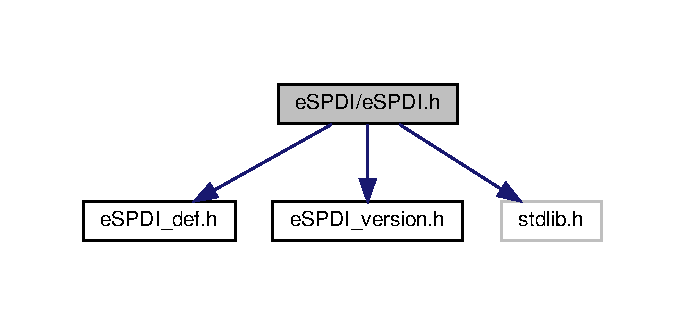
\includegraphics[width=329pt]{e_s_p_d_i_8h__incl}
\end{center}
\end{figure}
\subsection*{Functions}
\begin{DoxyCompactItemize}
\item 
int \hyperlink{e_s_p_d_i_8h_a50fc5a982da16e8f2a1505ad0d32aa1f}{A\+P\+C\+\_\+\+Init} (void $\ast$$\ast$pp\+Handle\+E\+Y\+SD, bool b\+Is\+Log\+Enabled)
\begin{DoxyCompactList}\small\item\em entry point of E\+Y\+SD camera S\+DK including 1.\+create a C\+E\+Y\+SD class for accessing oncming A\+P\+Is 2.\+find out E\+Y\+SD devices 3.\+create a C\+Video\+Device class for video streaming and hardware access \end{DoxyCompactList}\item 
int \hyperlink{e_s_p_d_i_8h_aedd81bb3e14bc88dd11f32d3542758e5}{A\+P\+C\+\_\+\+Find\+Device} (void $\ast$p\+Handle\+E\+Y\+SD)
\begin{DoxyCompactList}\small\item\em find out all E\+Y\+SD U\+SB devices by P\+ID, V\+ID and Chip\+ID, also remember device types \end{DoxyCompactList}\item 
void \hyperlink{e_s_p_d_i_8h_a426c58a17729a0eef9bea9d6b1d83d0f}{A\+P\+C\+\_\+\+Release} (void $\ast$$\ast$pp\+Handle\+E\+Y\+SD)
\begin{DoxyCompactList}\small\item\em release resource that A\+P\+C\+\_\+\+Init had allocated \end{DoxyCompactList}\item 
int \hyperlink{e_s_p_d_i_8h_a68b29f4a0036d0f30c424200439d08f5}{A\+P\+C\+\_\+\+Refresh\+Device} (void $\ast$p\+Handle\+E\+Y\+SD)
\begin{DoxyCompactList}\small\item\em refresh all E\+Y\+SD U\+VC devices \end{DoxyCompactList}\item 
int \hyperlink{e_s_p_d_i_8h_a0de92d6d9db8e34d9d9e44217520622d}{A\+P\+C\+\_\+\+Switch\+Baseline} (int index)
\begin{DoxyCompactList}\small\item\em Swich the baseline index. \end{DoxyCompactList}\item 
bool \hyperlink{e_s_p_d_i_8h_a6d8b3f6d6726e328e2138476429babde}{A\+P\+C\+\_\+\+Is\+M\+L\+Base\+Line} (void $\ast$p\+Handle\+E\+Y\+SD, \hyperlink{structtag_d_e_v_s_e_l}{P\+D\+E\+V\+S\+E\+L\+I\+N\+FO} p\+Dev\+Sel\+Info)
\begin{DoxyCompactList}\small\item\em Check the device is multiple baseline device. \end{DoxyCompactList}\item 
int \hyperlink{e_s_p_d_i_8h_a34eded6e88df666ec126e249da74b418}{A\+P\+C\+\_\+\+Do\+Fusion} (unsigned char $\ast$$\ast$p\+Depth\+Buf\+List, double $\ast$p\+Depth\+Merge, unsigned char $\ast$p\+Depth\+Merge\+Flag, int n\+D\+Width, int n\+D\+Height, double f\+Focus, double $\ast$p\+Baseline, double $\ast$p\+W\+R\+Near, double $\ast$p\+W\+R\+Far, double $\ast$p\+W\+R\+Fusion, int n\+Merge\+Num, bool bdepth2\+Byte11bit, int method)
\begin{DoxyCompactList}\small\item\em Do Fusion Merge. \end{DoxyCompactList}\item 
int \hyperlink{e_s_p_d_i_8h_a3f4bd97cd6a6684acddba10c5af172b8}{A\+P\+C\+\_\+\+Get\+Device\+Number} (void $\ast$p\+Handle\+E\+Y\+SD)
\begin{DoxyCompactList}\small\item\em get E\+Y\+SD U\+SB device numbers \end{DoxyCompactList}\item 
int \hyperlink{e_s_p_d_i_8h_ada8d1c7c13a01a947df9a5b4986e7753}{A\+P\+C\+\_\+\+Get\+Device\+Info} (void $\ast$p\+Handle\+E\+Y\+SD, \hyperlink{structtag_d_e_v_s_e_l}{P\+D\+E\+V\+S\+E\+L\+I\+N\+FO} p\+Dev\+Sel\+Info, \hyperlink{structtag_d_e_v_i_n_f_o_r_m_a_t_i_o_n}{D\+E\+V\+I\+N\+F\+O\+R\+M\+A\+T\+I\+ON} $\ast$pdevinfo)
\begin{DoxyCompactList}\small\item\em get informations of E\+Y\+SD U\+VC devices, see D\+E\+V\+I\+N\+F\+O\+R\+M\+A\+T\+I\+ON \end{DoxyCompactList}\item 
int \hyperlink{e_s_p_d_i_8h_a57912fe9a973f0d63298ace867853536}{A\+P\+C\+\_\+\+Get\+Device\+Info\+M\+B\+L\+\_\+15cm} (void $\ast$p\+Handle\+E\+Y\+SD, \hyperlink{structtag_d_e_v_s_e_l}{P\+D\+E\+V\+S\+E\+L\+I\+N\+FO} p\+Dev\+Sel\+Info, \hyperlink{structtag_d_e_v_i_n_f_o_r_m_a_t_i_o_n}{D\+E\+V\+I\+N\+F\+O\+R\+M\+A\+T\+I\+ON} $\ast$pdevinfo)
\begin{DoxyCompactList}\small\item\em get informations of E\+Y\+SD U\+VC devices, see D\+E\+V\+I\+N\+F\+O\+R\+M\+A\+T\+I\+ON \end{DoxyCompactList}\item 
int \hyperlink{e_s_p_d_i_8h_a1b94f15b46e4aaa159e422875eb9158b}{A\+P\+C\+\_\+\+Select\+Device} (void $\ast$p\+Handle\+E\+Y\+SD, int dev\+\_\+index)
\begin{DoxyCompactList}\small\item\em do not support currently \end{DoxyCompactList}\item 
bool \hyperlink{e_s_p_d_i_8h_adbd6fd827bf4a5425de95d938bc06f94}{A\+P\+C\+\_\+\+Is\+Interleave\+Device} (void $\ast$p\+Handle\+E\+Y\+SD, \hyperlink{structtag_d_e_v_s_e_l}{P\+D\+E\+V\+S\+E\+L\+I\+N\+FO} p\+Dev\+Sel\+Info)
\begin{DoxyCompactList}\small\item\em check module support interleave function or not \end{DoxyCompactList}\item 
int \hyperlink{e_s_p_d_i_8h_aed46003a2b1dbbfe05bf241e014b5500}{A\+P\+C\+\_\+\+Enable\+Interleave} (void $\ast$p\+Handle\+E\+Y\+SD, \hyperlink{structtag_d_e_v_s_e_l}{P\+D\+E\+V\+S\+E\+L\+I\+N\+FO} p\+Dev\+Sel\+Info, bool enable)
\begin{DoxyCompactList}\small\item\em enable or disable interleave function \end{DoxyCompactList}\item 
int \hyperlink{e_s_p_d_i_8h_ab73e91ef96a1f7fa4414d0719b62d0e0}{A\+P\+C\+\_\+\+Set\+Control\+Counter\+Mode} (void $\ast$p\+Handle\+E\+Y\+SD, \hyperlink{structtag_d_e_v_s_e_l}{P\+D\+E\+V\+S\+E\+L\+I\+N\+FO} p\+Dev\+Sel\+Info, unsigned char n\+Value)
\begin{DoxyCompactList}\small\item\em enable or disable interleave function \end{DoxyCompactList}\item 
int \hyperlink{e_s_p_d_i_8h_ad8a69db883662c07cb2c24f69efab041}{A\+P\+C\+\_\+\+Get\+Control\+Counter\+Mode} (void $\ast$p\+Handle\+E\+Y\+SD, \hyperlink{structtag_d_e_v_s_e_l}{P\+D\+E\+V\+S\+E\+L\+I\+N\+FO} p\+Dev\+Sel\+Info, unsigned char $\ast$n\+Value)
\begin{DoxyCompactList}\small\item\em enable or disable interleave function \end{DoxyCompactList}\item 
int \hyperlink{e_s_p_d_i_8h_a632143ad9bbcc8b1c5392c8d707ba538}{A\+P\+C\+\_\+\+Get\+Sensor\+Register} (void $\ast$p\+Handle\+E\+Y\+SD, \hyperlink{structtag_d_e_v_s_e_l}{P\+D\+E\+V\+S\+E\+L\+I\+N\+FO} p\+Dev\+Sel\+Info, int n\+Id, unsigned short address, unsigned short $\ast$p\+Value, int flag, S\+E\+N\+S\+O\+R\+M\+O\+D\+E\+\_\+\+I\+N\+FO Sensor\+Mode)
\item 
int \hyperlink{e_s_p_d_i_8h_a56c550c5b77f18460c082f24ed5030e1}{A\+P\+C\+\_\+\+Set\+Sensor\+Register} (void $\ast$p\+Handle\+E\+Y\+SD, \hyperlink{structtag_d_e_v_s_e_l}{P\+D\+E\+V\+S\+E\+L\+I\+N\+FO} p\+Dev\+Sel\+Info, int n\+Id, unsigned short address, unsigned short n\+Value, int flag, S\+E\+N\+S\+O\+R\+M\+O\+D\+E\+\_\+\+I\+N\+FO Sensor\+Mode)
\begin{DoxyCompactList}\small\item\em set sensor register value \end{DoxyCompactList}\item 
int \hyperlink{e_s_p_d_i_8h_adaba7fb1a61ca589aa3ffe6a55a3bcb5}{A\+P\+C\+\_\+\+Get\+F\+W\+Register} (void $\ast$p\+Handle\+E\+Y\+SD, \hyperlink{structtag_d_e_v_s_e_l}{P\+D\+E\+V\+S\+E\+L\+I\+N\+FO} p\+Dev\+Sel\+Info, unsigned short address, unsigned short $\ast$p\+Value, int flag)
\begin{DoxyCompactList}\small\item\em get firmware register value \end{DoxyCompactList}\item 
int \hyperlink{e_s_p_d_i_8h_ab7ee0aa5efbf2643c2ed60f3d297fac1}{A\+P\+C\+\_\+\+Set\+F\+W\+Register} (void $\ast$p\+Handle\+E\+Y\+SD, \hyperlink{structtag_d_e_v_s_e_l}{P\+D\+E\+V\+S\+E\+L\+I\+N\+FO} p\+Dev\+Sel\+Info, unsigned short address, unsigned short n\+Value, int flag)
\begin{DoxyCompactList}\small\item\em set firmware register value \end{DoxyCompactList}\item 
int \hyperlink{e_s_p_d_i_8h_ad47dd05fe99d320c85172a653d6c6d23}{A\+P\+C\+\_\+\+Get\+H\+W\+Register} (void $\ast$p\+Handle\+E\+Y\+SD, \hyperlink{structtag_d_e_v_s_e_l}{P\+D\+E\+V\+S\+E\+L\+I\+N\+FO} p\+Dev\+Sel\+Info, unsigned short address, unsigned short $\ast$p\+Value, int flag)
\begin{DoxyCompactList}\small\item\em get hardware register value \end{DoxyCompactList}\item 
int \hyperlink{e_s_p_d_i_8h_a19d698ae63d4fe3a39298ae9660011aa}{A\+P\+C\+\_\+\+Set\+H\+W\+Register} (void $\ast$p\+Handle\+E\+Y\+SD, \hyperlink{structtag_d_e_v_s_e_l}{P\+D\+E\+V\+S\+E\+L\+I\+N\+FO} p\+Dev\+Sel\+Info, unsigned short address, unsigned short n\+Value, int flag)
\begin{DoxyCompactList}\small\item\em set hardware register \end{DoxyCompactList}\item 
int \hyperlink{e_s_p_d_i_8h_a40b5715d62526943483b0b5d249bc647}{A\+P\+C\+\_\+\+Get\+Multi\+Bytes\+H\+W\+Register} (void $\ast$p\+Handle\+E\+Y\+SD, \hyperlink{structtag_d_e_v_s_e_l}{P\+D\+E\+V\+S\+E\+L\+I\+N\+FO} p\+Dev\+Sel\+Info, unsigned short address, unsigned char $\ast$Data, int size, int flag)
\begin{DoxyCompactList}\small\item\em set hardware register \end{DoxyCompactList}\item 
int \hyperlink{e_s_p_d_i_8h_a0722345ea3e43ec7f54c7d4b701b3144}{A\+P\+C\+\_\+\+Set\+Multi\+Bytes\+H\+W\+Register} (void $\ast$p\+Handle\+E\+Y\+SD, \hyperlink{structtag_d_e_v_s_e_l}{P\+D\+E\+V\+S\+E\+L\+I\+N\+FO} p\+Dev\+Sel\+Info, unsigned short address, unsigned char $\ast$Data, int size, int flag)
\begin{DoxyCompactList}\small\item\em set hardware register \end{DoxyCompactList}\item 
int \hyperlink{e_s_p_d_i_8h_a31eeaacd17fffe9c5bd80e1a4f60b4e2}{A\+P\+C\+\_\+\+Get\+Bus\+Info} (void $\ast$p\+Handle\+E\+Y\+SD, \hyperlink{structtag_d_e_v_s_e_l}{P\+D\+E\+V\+S\+E\+L\+I\+N\+FO} p\+Dev\+Sel\+Info, char $\ast$psz\+Bus\+Info, int $\ast$p\+Actual\+Length)
\begin{DoxyCompactList}\small\item\em get the firmware version of device, the version is a string \end{DoxyCompactList}\item 
int \hyperlink{e_s_p_d_i_8h_ade99a1838931b2d06ac09ffebc0810fd}{A\+P\+C\+\_\+\+Get\+Fw\+Version} (void $\ast$p\+Handle\+E\+Y\+SD, \hyperlink{structtag_d_e_v_s_e_l}{P\+D\+E\+V\+S\+E\+L\+I\+N\+FO} p\+Dev\+Sel\+Info, char $\ast$psz\+Fw\+Version, int n\+Buffer\+Size, int $\ast$p\+Actual\+Length)
\begin{DoxyCompactList}\small\item\em get the firmware version of device, the version is a string \end{DoxyCompactList}\item 
int \hyperlink{e_s_p_d_i_8h_ae8116f0570fa3f756129d06275ff9b0d}{A\+P\+C\+\_\+\+Get\+Pid\+Vid} (void $\ast$p\+Handle\+E\+Y\+SD, \hyperlink{structtag_d_e_v_s_e_l}{P\+D\+E\+V\+S\+E\+L\+I\+N\+FO} p\+Dev\+Sel\+Info, unsigned short $\ast$p\+Pid\+Buf, unsigned short $\ast$p\+Vid\+Buf)
\begin{DoxyCompactList}\small\item\em get P\+I\+D(product I\+D) and V\+I\+D(vendor I\+D) of device \end{DoxyCompactList}\item 
int \hyperlink{e_s_p_d_i_8h_acb665df80c6fe114534d3a391df777fb}{A\+P\+C\+\_\+\+Set\+Pid\+Vid} (void $\ast$p\+Handle\+E\+Y\+SD, \hyperlink{structtag_d_e_v_s_e_l}{P\+D\+E\+V\+S\+E\+L\+I\+N\+FO} p\+Dev\+Sel\+Info, unsigned short $\ast$p\+Pid\+Buf, unsigned short $\ast$p\+Vid\+Buf)
\begin{DoxyCompactList}\small\item\em set P\+ID and V\+ID to device \end{DoxyCompactList}\item 
int \hyperlink{e_s_p_d_i_8h_a5be2b5453bbfb5bd7ba6437747cb504e}{A\+P\+C\+\_\+\+Get\+Serial\+Number} (void $\ast$p\+Handle\+E\+Y\+SD, \hyperlink{structtag_d_e_v_s_e_l}{P\+D\+E\+V\+S\+E\+L\+I\+N\+FO} p\+Dev\+Sel\+Info, unsigned char $\ast$p\+Data, int nbuffer\+Size, int $\ast$p\+Len)
\begin{DoxyCompactList}\small\item\em get device serial number \end{DoxyCompactList}\item 
int \hyperlink{e_s_p_d_i_8h_a9e051b33c43f02d0531eaf71516bc579}{A\+P\+C\+\_\+\+Set\+Serial\+Number} (void $\ast$p\+Handle\+E\+Y\+SD, \hyperlink{structtag_d_e_v_s_e_l}{P\+D\+E\+V\+S\+E\+L\+I\+N\+FO} p\+Dev\+Sel\+Info, unsigned char $\ast$p\+Data, int n\+Len)
\begin{DoxyCompactList}\small\item\em set serial number to device \end{DoxyCompactList}\item 
int \hyperlink{e_s_p_d_i_8h_a67592a7cc13d23de5099d68fd295b11c}{A\+P\+C\+\_\+\+Get\+Y\+Offset} (void $\ast$p\+Handle\+E\+Y\+SD, \hyperlink{structtag_d_e_v_s_e_l}{P\+D\+E\+V\+S\+E\+L\+I\+N\+FO} p\+Dev\+Sel\+Info, B\+Y\+TE $\ast$buffer, int Buffer\+Length, int $\ast$p\+Actual\+Length, int index)
\begin{DoxyCompactList}\small\item\em get Y offset (file ID 30+) value \end{DoxyCompactList}\item 
int \hyperlink{e_s_p_d_i_8h_ab2b5b138c8ebc18c26e330b3afce0d24}{A\+P\+C\+\_\+\+Get\+Rectify\+Table} (void $\ast$p\+Handle\+E\+Y\+SD, \hyperlink{structtag_d_e_v_s_e_l}{P\+D\+E\+V\+S\+E\+L\+I\+N\+FO} p\+Dev\+Sel\+Info, B\+Y\+TE $\ast$buffer, int Buffer\+Length, int $\ast$p\+Actual\+Length, int index)
\begin{DoxyCompactList}\small\item\em get rectify values (file ID 40+) from flash \end{DoxyCompactList}\item 
int \hyperlink{e_s_p_d_i_8h_a8862f5a1bcb725dceed48d1a38521227}{A\+P\+C\+\_\+\+Get\+Z\+D\+Table} (void $\ast$p\+Handle\+E\+Y\+SD, \hyperlink{structtag_d_e_v_s_e_l}{P\+D\+E\+V\+S\+E\+L\+I\+N\+FO} p\+Dev\+Sel\+Info, B\+Y\+TE $\ast$buffer, int Buffer\+Length, int $\ast$p\+Actual\+Length, \hyperlink{structtag_z_d_table_info}{P\+Z\+D\+T\+A\+B\+L\+E\+I\+N\+FO} p\+Z\+D\+Table\+Info)
\begin{DoxyCompactList}\small\item\em get disparity and Z values from flash \end{DoxyCompactList}\item 
int \hyperlink{e_s_p_d_i_8h_a51517b84ea88502f466b7c9e177b35b3}{A\+P\+C\+\_\+\+Get\+Log\+Data} (void $\ast$p\+Handle\+E\+Y\+SD, \hyperlink{structtag_d_e_v_s_e_l}{P\+D\+E\+V\+S\+E\+L\+I\+N\+FO} p\+Dev\+Sel\+Info, B\+Y\+TE $\ast$buffer, int Buffer\+Length, int $\ast$p\+Actual\+Length, int index, C\+A\+L\+I\+B\+R\+A\+T\+I\+O\+N\+\_\+\+L\+O\+G\+\_\+\+T\+Y\+PE type)
\begin{DoxyCompactList}\small\item\em get log data from flash \end{DoxyCompactList}\item 
int \hyperlink{e_s_p_d_i_8h_ac62ff60199e614c76f13d457f21e9632}{A\+P\+C\+\_\+\+Get\+User\+Data} (void $\ast$p\+Handle\+E\+Y\+SD, \hyperlink{structtag_d_e_v_s_e_l}{P\+D\+E\+V\+S\+E\+L\+I\+N\+FO} p\+Dev\+Sel\+Info, B\+Y\+TE $\ast$buffer, int Buffer\+Length, U\+S\+E\+R\+D\+A\+T\+A\+\_\+\+S\+E\+C\+T\+I\+O\+N\+\_\+\+I\+N\+D\+EX usi)
\begin{DoxyCompactList}\small\item\em get user data from flash \end{DoxyCompactList}\item 
int \hyperlink{e_s_p_d_i_8h_a20ac8010fd3795c8d73fb685fa72419f}{A\+P\+C\+\_\+\+Set\+Y\+Offset} (void $\ast$p\+Handle\+E\+Y\+SD, \hyperlink{structtag_d_e_v_s_e_l}{P\+D\+E\+V\+S\+E\+L\+I\+N\+FO} p\+Dev\+Sel\+Info, B\+Y\+TE $\ast$buffer, int Buffer\+Length, int $\ast$p\+Actual\+Length, int index)
\begin{DoxyCompactList}\small\item\em set Y offset values \end{DoxyCompactList}\item 
int \hyperlink{e_s_p_d_i_8h_a9f99f7a1656a99418a8a8755c0b9cad1}{A\+P\+C\+\_\+\+Set\+Rectify\+Table} (void $\ast$p\+Handle\+E\+Y\+SD, \hyperlink{structtag_d_e_v_s_e_l}{P\+D\+E\+V\+S\+E\+L\+I\+N\+FO} p\+Dev\+Sel\+Info, B\+Y\+TE $\ast$buffer, int Buffer\+Length, int $\ast$p\+Actual\+Length, int index)
\begin{DoxyCompactList}\small\item\em set rectify values to flash \end{DoxyCompactList}\item 
int \hyperlink{e_s_p_d_i_8h_acaa58e000752066086147c4280bec2e5}{A\+P\+C\+\_\+\+Set\+Z\+D\+Table} (void $\ast$p\+Handle\+E\+Y\+SD, \hyperlink{structtag_d_e_v_s_e_l}{P\+D\+E\+V\+S\+E\+L\+I\+N\+FO} p\+Dev\+Sel\+Info, B\+Y\+TE $\ast$buffer, int Buffer\+Length, int $\ast$p\+Actual\+Length, \hyperlink{structtag_z_d_table_info}{P\+Z\+D\+T\+A\+B\+L\+E\+I\+N\+FO} p\+Z\+D\+Table\+Info)
\begin{DoxyCompactList}\small\item\em set disparity and Z values to flash \end{DoxyCompactList}\item 
int \hyperlink{e_s_p_d_i_8h_a33e62e35695987eecf14c5293ae76195}{A\+P\+C\+\_\+\+Set\+Log\+Data} (void $\ast$p\+Handle\+E\+Y\+SD, \hyperlink{structtag_d_e_v_s_e_l}{P\+D\+E\+V\+S\+E\+L\+I\+N\+FO} p\+Dev\+Sel\+Info, B\+Y\+TE $\ast$buffer, int Buffer\+Length, int $\ast$p\+Actual\+Length, int index)
\begin{DoxyCompactList}\small\item\em set log data to flash \end{DoxyCompactList}\item 
int \hyperlink{e_s_p_d_i_8h_a065c9444738bfadbc19edb84278acd0b}{A\+P\+C\+\_\+\+Set\+User\+Data} (void $\ast$p\+Handle\+E\+Y\+SD, \hyperlink{structtag_d_e_v_s_e_l}{P\+D\+E\+V\+S\+E\+L\+I\+N\+FO} p\+Dev\+Sel\+Info, B\+Y\+TE $\ast$buffer, int Buffer\+Length, U\+S\+E\+R\+D\+A\+T\+A\+\_\+\+S\+E\+C\+T\+I\+O\+N\+\_\+\+I\+N\+D\+EX usi)
\begin{DoxyCompactList}\small\item\em set user data to flash \end{DoxyCompactList}\item 
int \hyperlink{e_s_p_d_i_8h_ab86e5fe0586a7fc0e31bc0b023582bdd}{A\+P\+C\+\_\+\+Read\+Flash\+Data} (void $\ast$p\+Handle\+E\+Y\+SD, \hyperlink{structtag_d_e_v_s_e_l}{P\+D\+E\+V\+S\+E\+L\+I\+N\+FO} p\+Dev\+Sel\+Info, F\+L\+A\+S\+H\+\_\+\+D\+A\+T\+A\+\_\+\+T\+Y\+PE fdt, B\+Y\+TE $\ast$p\+Buffer, unsigned long int Buffer\+Length, unsigned long int $\ast$p\+Actual\+Length)
\begin{DoxyCompactList}\small\item\em read firmware code(.bin) form flash The firmware code is the combination of boot loader, firmware body and plug-\/in data. This input buffer length has to match with the flash data type \end{DoxyCompactList}\item 
int \hyperlink{e_s_p_d_i_8h_ae753d2551ae604b928070fa7d4878cfd}{A\+P\+C\+\_\+\+Write\+Flash\+Data} (void $\ast$p\+Handle\+E\+Y\+SD, \hyperlink{structtag_d_e_v_s_e_l}{P\+D\+E\+V\+S\+E\+L\+I\+N\+FO} p\+Dev\+Sel\+Info, F\+L\+A\+S\+H\+\_\+\+D\+A\+T\+A\+\_\+\+T\+Y\+PE fdt, B\+Y\+TE $\ast$p\+Buffer, unsigned long int Buffer\+Length, bool b\+Is\+Data\+Verify, \hyperlink{structtag_k_e_e_p___d_a_t_a___c_t_r_l}{K\+E\+E\+P\+\_\+\+D\+A\+T\+A\+\_\+\+C\+T\+RL} kdc)
\begin{DoxyCompactList}\small\item\em write firmware code(.bin) to flash The firmware code is the combination of boot loader, firmware body and plug-\/in data, also can keep original functions(Serial Number, Sensor Position, Rectification\+Table, ZD Table and Calibration\+Log) on camera flash by K\+E\+E\+P\+\_\+\+D\+A\+T\+A\+\_\+\+C\+T\+RL control \end{DoxyCompactList}\item 
\mbox{\Hypertarget{e_s_p_d_i_8h_ae075b17431c5aa28c89dc6c5b83ac2b2}\label{e_s_p_d_i_8h_ae075b17431c5aa28c89dc6c5b83ac2b2}} 
int \hyperlink{e_s_p_d_i_8h_ae075b17431c5aa28c89dc6c5b83ac2b2}{A\+P\+C\+\_\+\+Get\+Device\+Port\+Type} (void $\ast$p\+Handle\+E\+Y\+SD, \hyperlink{structtag_d_e_v_s_e_l}{P\+D\+E\+V\+S\+E\+L\+I\+N\+FO} p\+Dev\+Sel\+Info, U\+S\+B\+\_\+\+P\+O\+R\+T\+\_\+\+T\+Y\+PE $\ast$p\+U\+S\+B\+\_\+\+Port\+\_\+\+Type)
\begin{DoxyCompactList}\small\item\em Get Device U\+S\+B-\/port-\/type. \end{DoxyCompactList}\item 
int \hyperlink{e_s_p_d_i_8h_a32320100fdbc7d1ae2115c1e902d8b7c}{A\+P\+C\+\_\+\+Get\+Device\+Resolution\+List} (void $\ast$p\+Handle\+E\+Y\+SD, \hyperlink{structtag_d_e_v_s_e_l}{P\+D\+E\+V\+S\+E\+L\+I\+N\+FO} p\+Dev\+Sel\+Info, int n\+Max\+Count, \hyperlink{structtag_a_p_c___s_t_r_e_a_m___i_n_f_o}{A\+P\+C\+\_\+\+S\+T\+R\+E\+A\+M\+\_\+\+I\+N\+FO} $\ast$p\+Stream\+Info0, int n\+Max\+Cvoidount1, \hyperlink{structtag_a_p_c___s_t_r_e_a_m___i_n_f_o}{A\+P\+C\+\_\+\+S\+T\+R\+E\+A\+M\+\_\+\+I\+N\+FO} $\ast$p\+Stream\+Info1)
\begin{DoxyCompactList}\small\item\em get the device resolution list \end{DoxyCompactList}\item 
int \hyperlink{e_s_p_d_i_8h_a60c7da1769a334fec9519bb737bbb1b3}{A\+P\+C\+\_\+\+Setup\+\_\+v4l2\+\_\+requestbuffers} (void $\ast$p\+Handle\+E\+Y\+SD, \hyperlink{structtag_d_e_v_s_e_l}{P\+D\+E\+V\+S\+E\+L\+I\+N\+FO} p\+Dev\+Sel\+Info, int cnt)
\begin{DoxyCompactList}\small\item\em Setup v4l2 request buffers, default = 4. \end{DoxyCompactList}\item 
int \hyperlink{e_s_p_d_i_8h_a5d004ffbd4bee13133380f7ff02e8bb1}{A\+P\+C\+\_\+\+Open\+Device} (void $\ast$p\+Handle\+E\+Y\+SD, \hyperlink{structtag_d_e_v_s_e_l}{P\+D\+E\+V\+S\+E\+L\+I\+N\+FO} p\+Dev\+Sel\+Info, int n\+E\+P0\+Width, int n\+E\+P0\+Height, bool b\+E\+P0\+M\+J\+PG, int n\+E\+P1\+Width, int n\+E\+P1\+Height, D\+E\+P\+T\+H\+\_\+\+T\+R\+A\+N\+S\+F\+E\+R\+\_\+\+C\+T\+RL dtc=D\+E\+P\+T\+H\+\_\+\+I\+M\+G\+\_\+\+N\+O\+N\+\_\+\+T\+R\+A\+N\+S\+F\+ER, bool b\+Is\+Output\+R\+G\+B24=false, void $\ast$ph\+Wnd\+Notice=0, int $\ast$p\+F\+PS=0, C\+O\+N\+T\+R\+O\+L\+\_\+\+M\+O\+DE cm=I\+M\+A\+G\+E\+\_\+\+S\+N\+\_\+\+N\+O\+N\+S\+Y\+NC)
\begin{DoxyCompactList}\small\item\em the implement layer to open E\+Y\+SD camera device by V4\+L2(\href{https://en.wikipedia.org/wiki/Video4Linux}{\tt https\+://en.\+wikipedia.\+org/wiki/\+Video4\+Linux}), can open color and depth at one time call, do functions as below, \end{DoxyCompactList}\item 
int \hyperlink{e_s_p_d_i_8h_a5a4a4e47fbe46537ad4630723583a003}{A\+P\+C\+\_\+\+Open\+Device2} (void $\ast$p\+Handle\+E\+Y\+SD, \hyperlink{structtag_d_e_v_s_e_l}{P\+D\+E\+V\+S\+E\+L\+I\+N\+FO} p\+Dev\+Sel\+Info, int n\+E\+P0\+Width, int n\+E\+P0\+Height, bool b\+E\+P0\+M\+J\+PG, int n\+E\+P1\+Width, int n\+E\+P1\+Height, D\+E\+P\+T\+H\+\_\+\+T\+R\+A\+N\+S\+F\+E\+R\+\_\+\+C\+T\+RL dtc=D\+E\+P\+T\+H\+\_\+\+I\+M\+G\+\_\+\+N\+O\+N\+\_\+\+T\+R\+A\+N\+S\+F\+ER, bool b\+Is\+Output\+R\+G\+B24=false, void $\ast$ph\+Wnd\+Notice=0, int $\ast$p\+F\+PS=0, C\+O\+N\+T\+R\+O\+L\+\_\+\+M\+O\+DE cm=I\+M\+A\+G\+E\+\_\+\+S\+N\+\_\+\+N\+O\+N\+S\+Y\+NC)
\begin{DoxyCompactList}\small\item\em the implement layer to open E\+Y\+SD camera device by V4\+L2(\href{https://en.wikipedia.org/wiki/Video4Linux}{\tt https\+://en.\+wikipedia.\+org/wiki/\+Video4\+Linux}), can open color and depth at one time call, do functions as below, \end{DoxyCompactList}\item 
int \hyperlink{e_s_p_d_i_8h_aa24fa13dbdb16bcd550991a7cc267d6c}{A\+P\+C\+\_\+\+Open\+Device\+M\+BL} (void $\ast$p\+Handle\+E\+Y\+SD, \hyperlink{structtag_d_e_v_s_e_l}{P\+D\+E\+V\+S\+E\+L\+I\+N\+FO} p\+Dev\+Sel\+Info, int n\+E\+P0\+Width, int n\+E\+P0\+Height, bool b\+E\+P0\+M\+J\+PG, int n\+E\+P1\+Width, int n\+E\+P1\+Height, D\+E\+P\+T\+H\+\_\+\+T\+R\+A\+N\+S\+F\+E\+R\+\_\+\+C\+T\+RL dtc=D\+E\+P\+T\+H\+\_\+\+I\+M\+G\+\_\+\+N\+O\+N\+\_\+\+T\+R\+A\+N\+S\+F\+ER, bool b\+Is\+Output\+R\+G\+B24=false, void $\ast$ph\+Wnd\+Notice=0, int $\ast$p\+F\+PS=0, C\+O\+N\+T\+R\+O\+L\+\_\+\+M\+O\+DE cm=I\+M\+A\+G\+E\+\_\+\+S\+N\+\_\+\+N\+O\+N\+S\+Y\+NC)
\begin{DoxyCompactList}\small\item\em the implement layer to open Multiple Base Line E\+Y\+SD camera device by V4\+L2(\href{https://en.wikipedia.org/wiki/Video4Linux}{\tt https\+://en.\+wikipedia.\+org/wiki/\+Video4\+Linux}), can open color and depth at one time call, do functions as below, \end{DoxyCompactList}\item 
int \hyperlink{e_s_p_d_i_8h_a5c6742c79acbc5381b172cc24895d5b7}{A\+P\+C\+\_\+\+Close\+Device\+M\+BL} (void $\ast$p\+Handle\+E\+Y\+SD, \hyperlink{structtag_d_e_v_s_e_l}{P\+D\+E\+V\+S\+E\+L\+I\+N\+FO} p\+Dev\+Sel\+Info)
\begin{DoxyCompactList}\small\item\em close Multiple Base Linedevice and free resource \end{DoxyCompactList}\item 
int \hyperlink{e_s_p_d_i_8h_a1723b49dd5783db98f12bfbe2f0933d5}{A\+P\+C\+\_\+\+Close\+Device} (void $\ast$p\+Handle\+E\+Y\+SD, \hyperlink{structtag_d_e_v_s_e_l}{P\+D\+E\+V\+S\+E\+L\+I\+N\+FO} p\+Dev\+Sel\+Info)
\begin{DoxyCompactList}\small\item\em close device and free resource \end{DoxyCompactList}\item 
int \hyperlink{e_s_p_d_i_8h_a9158d00c8ecbc952b076c07f7fa88fb7}{A\+P\+C\+\_\+\+Close\+Device\+Ex} (void $\ast$p\+Handle\+E\+Y\+SD, \hyperlink{structtag_d_e_v_s_e_l}{P\+D\+E\+V\+S\+E\+L\+I\+N\+FO} p\+Dev\+Sel\+Info)
\begin{DoxyCompactList}\small\item\em close device and free resource for warm reset \end{DoxyCompactList}\item 
int \hyperlink{e_s_p_d_i_8h_aabc7575da7cdfd61ca72ad653a58a745}{A\+P\+C\+\_\+\+Get\+Image} (void $\ast$p\+Handle\+E\+Y\+SD, \hyperlink{structtag_d_e_v_s_e_l}{P\+D\+E\+V\+S\+E\+L\+I\+N\+FO} p\+Dev\+Sel\+Info, B\+Y\+TE $\ast$p\+Buf, unsigned long int $\ast$p\+Image\+Size, int $\ast$p\+Serial=0, int n\+Depth\+Data\+Type=0)
\begin{DoxyCompactList}\small\item\em get color or depth pin image by issuing V4\+L2\textquotesingle{}s I\+O\+C\+TL to get frame data \end{DoxyCompactList}\item 
int \hyperlink{e_s_p_d_i_8h_af25a1d8b7cc5d267de29f50b6cb28226}{A\+P\+C\+\_\+\+Get\+Color\+Image} (void $\ast$p\+Handle\+E\+Y\+SD, \hyperlink{structtag_d_e_v_s_e_l}{P\+D\+E\+V\+S\+E\+L\+I\+N\+FO} p\+Dev\+Sel\+Info, B\+Y\+TE $\ast$p\+Buf, unsigned long int $\ast$p\+Image\+Size, int $\ast$p\+Serial=0, int n\+Depth\+Data\+Type=0)
\begin{DoxyCompactList}\small\item\em get color image by issuing V4\+L2\textquotesingle{}s I\+O\+C\+TL to get frame data \end{DoxyCompactList}\item 
int \hyperlink{e_s_p_d_i_8h_ae2c6d1d20deb690868dcc605492b6e7c}{A\+P\+C\+\_\+\+Get\+Color\+Image\+With\+Timestamp} (void $\ast$p\+Handle\+E\+Y\+SD, \hyperlink{structtag_d_e_v_s_e_l}{P\+D\+E\+V\+S\+E\+L\+I\+N\+FO} p\+Dev\+Sel\+Info, B\+Y\+TE $\ast$p\+Buf, unsigned long int $\ast$p\+Image\+Size, int $\ast$p\+Serial, int n\+Depth\+Data\+Type, int64\+\_\+t $\ast$pcur\+\_\+tv\+\_\+sec, int64\+\_\+t $\ast$pcur\+\_\+tv\+\_\+usec)
\begin{DoxyCompactList}\small\item\em get color image by issuing V4\+L2\textquotesingle{}s I\+O\+C\+TL to get frame data \end{DoxyCompactList}\item 
int \hyperlink{e_s_p_d_i_8h_a4b8a8284e274b729aeb75b54bd0698e6}{A\+P\+C\+\_\+\+Get\+Depth\+Image} (void $\ast$p\+Handle\+E\+Y\+SD, \hyperlink{structtag_d_e_v_s_e_l}{P\+D\+E\+V\+S\+E\+L\+I\+N\+FO} p\+Dev\+Sel\+Info, B\+Y\+TE $\ast$p\+Buf, unsigned long int $\ast$p\+Image\+Size, int $\ast$p\+Serial=0, int n\+Depth\+Data\+Type=0)
\begin{DoxyCompactList}\small\item\em get depth image by issuing V4\+L2\textquotesingle{}s I\+O\+C\+TL to get frame data \end{DoxyCompactList}\item 
int \hyperlink{e_s_p_d_i_8h_aff378882668dc1438c4307a11f37d756}{A\+P\+C\+\_\+\+Get\+Depth\+Image\+With\+Timestamp} (void $\ast$p\+Handle\+E\+Y\+SD, \hyperlink{structtag_d_e_v_s_e_l}{P\+D\+E\+V\+S\+E\+L\+I\+N\+FO} p\+Dev\+Sel\+Info, B\+Y\+TE $\ast$p\+Buf, unsigned long int $\ast$p\+Image\+Size, int $\ast$p\+Serial, int n\+Depth\+Data\+Type, int64\+\_\+t $\ast$pcur\+\_\+tv\+\_\+sec, int64\+\_\+t $\ast$pcur\+\_\+tv\+\_\+usec)
\begin{DoxyCompactList}\small\item\em get color image by issuing V4\+L2\textquotesingle{}s I\+O\+C\+TL to get frame data \end{DoxyCompactList}\item 
int \hyperlink{e_s_p_d_i_8h_a39464b6aadc1788a66f81597992da104}{A\+P\+C\+\_\+\+Setup\+Block} (void $\ast$p\+Handle\+E\+Y\+SD, \hyperlink{structtag_d_e_v_s_e_l}{P\+D\+E\+V\+S\+E\+L\+I\+N\+FO} p\+Dev\+Sel\+Info, bool enable)
\begin{DoxyCompactList}\small\item\em get color or depth pin image by issuing V4\+L2\textquotesingle{}s I\+O\+C\+TL to get frame data \end{DoxyCompactList}\item 
int \hyperlink{e_s_p_d_i_8h_a7badeb2fa81efa920a4bb6cdb4254ad8}{A\+P\+C\+\_\+\+Get\+\_\+\+Color\+\_\+30\+\_\+mm\+\_\+depth} (void $\ast$p\+Handle\+E\+Y\+SD, \hyperlink{structtag_d_e_v_s_e_l}{P\+D\+E\+V\+S\+E\+L\+I\+N\+FO} p\+Dev\+Sel\+Info, B\+Y\+TE $\ast$p\+Buf, unsigned long int $\ast$p\+Image\+Size, int $\ast$p\+Serial=0, int n\+Depth\+Data\+Type=0)
\begin{DoxyCompactList}\small\item\em get color or depth pin image by issuing V4\+L2\textquotesingle{}s I\+O\+C\+TL to get frame data \end{DoxyCompactList}\item 
int \hyperlink{e_s_p_d_i_8h_a9de52f3eb861e19dc68abafa4d4e9068}{A\+P\+C\+\_\+\+Get\+\_\+60\+\_\+mm\+\_\+depth} (void $\ast$p\+Handle\+E\+Y\+SD, \hyperlink{structtag_d_e_v_s_e_l}{P\+D\+E\+V\+S\+E\+L\+I\+N\+FO} p\+Dev\+Sel\+Info, B\+Y\+TE $\ast$p\+Buf, unsigned long int $\ast$p\+Image\+Size, int $\ast$p\+Serial=0, int n\+Depth\+Data\+Type=0)
\begin{DoxyCompactList}\small\item\em get color or depth pin image by issuing V4\+L2\textquotesingle{}s I\+O\+C\+TL to get frame data \end{DoxyCompactList}\item 
int \hyperlink{e_s_p_d_i_8h_a7dedea5c2027b9de091cd3e97b0b0522}{A\+P\+C\+\_\+\+Get\+\_\+150\+\_\+mm\+\_\+depth} (void $\ast$p\+Handle\+E\+Y\+SD, \hyperlink{structtag_d_e_v_s_e_l}{P\+D\+E\+V\+S\+E\+L\+I\+N\+FO} p\+Dev\+Sel\+Info, B\+Y\+TE $\ast$p\+Buf, unsigned long int $\ast$p\+Image\+Size, int $\ast$p\+Serial=0, int n\+Depth\+Data\+Type=0)
\begin{DoxyCompactList}\small\item\em get color or depth pin image by issuing V4\+L2\textquotesingle{}s I\+O\+C\+TL to get frame data \end{DoxyCompactList}\item 
int \hyperlink{e_s_p_d_i_8h_a7ad661c1b40b139408e8f957145438e6}{A\+P\+C\+\_\+\+Get2\+Image} (void $\ast$p\+Handle\+E\+Y\+SD, \hyperlink{structtag_d_e_v_s_e_l}{P\+D\+E\+V\+S\+E\+L\+I\+N\+FO} p\+Dev\+Sel\+Info, B\+Y\+TE $\ast$p\+Color\+Img\+Buf, B\+Y\+TE $\ast$p\+Depth\+Img\+Buf, unsigned long int $\ast$p\+Color\+Image\+Size, unsigned long int $\ast$p\+Depth\+Image\+Size, int $\ast$p\+Serial=0, int $\ast$p\+Serial2=0, int n\+Depth\+Data\+Type=0)
\begin{DoxyCompactList}\small\item\em get color and/or depth pin images see A\+P\+C\+\_\+\+Get\+Image for detailed description \end{DoxyCompactList}\item 
int \hyperlink{e_s_p_d_i_8h_ac46eecfafb2a12af72def7495ea2ecb2}{A\+P\+C\+\_\+\+Get\+Exposure\+Time} (void $\ast$p\+Handle\+E\+Y\+SD, \hyperlink{structtag_d_e_v_s_e_l}{P\+D\+E\+V\+S\+E\+L\+I\+N\+FO} p\+Dev\+Sel\+Info, int n\+Sensor\+Mode, float $\ast$pf\+Exp\+Time\+MS)
\begin{DoxyCompactList}\small\item\em get exposure time of I\+SP setting in millisecond the target sensor type was set in \hyperlink{e_s_p_d_i_8h_a7ad9ac9ad61c820bc6177045b84b9649}{A\+P\+C\+\_\+\+Set\+Sensor\+Type\+Name()} \end{DoxyCompactList}\item 
int \hyperlink{e_s_p_d_i_8h_afbe3057be1fc18382e7446adb9ad6c55}{A\+P\+C\+\_\+\+Set\+Exposure\+Time} (void $\ast$p\+Handle\+E\+Y\+SD, \hyperlink{structtag_d_e_v_s_e_l}{P\+D\+E\+V\+S\+E\+L\+I\+N\+FO} p\+Dev\+Sel\+Info, int n\+Sensor\+Mode, float f\+Exp\+Time\+MS)
\begin{DoxyCompactList}\small\item\em set exposure time of I\+SP sensor setting the target sensor type was set in \hyperlink{e_s_p_d_i_8h_a7ad9ac9ad61c820bc6177045b84b9649}{A\+P\+C\+\_\+\+Set\+Sensor\+Type\+Name()} \end{DoxyCompactList}\item 
int \hyperlink{e_s_p_d_i_8h_a78de7b91f2c0864a664d9c37ea629709}{A\+P\+C\+\_\+\+Get\+Global\+Gain} (void $\ast$p\+Handle\+E\+Y\+SD, \hyperlink{structtag_d_e_v_s_e_l}{P\+D\+E\+V\+S\+E\+L\+I\+N\+FO} p\+Dev\+Sel\+Info, int n\+Sensor\+Mode, float $\ast$pf\+Global\+Gain)
\begin{DoxyCompactList}\small\item\em get global gain of I\+SP setting the target sensor type was set in \hyperlink{e_s_p_d_i_8h_a7ad9ac9ad61c820bc6177045b84b9649}{A\+P\+C\+\_\+\+Set\+Sensor\+Type\+Name()} \end{DoxyCompactList}\item 
int \hyperlink{e_s_p_d_i_8h_a2ef4fc7b9542ee31f5ec52bd5bfe697a}{A\+P\+C\+\_\+\+Set\+Global\+Gain} (void $\ast$p\+Handle\+E\+Y\+SD, \hyperlink{structtag_d_e_v_s_e_l}{P\+D\+E\+V\+S\+E\+L\+I\+N\+FO} p\+Dev\+Sel\+Info, int n\+Sensor\+Mode, float f\+Global\+Gain)
\begin{DoxyCompactList}\small\item\em set global gain of I\+SP sensor setting the target sensor type was set in \hyperlink{e_s_p_d_i_8h_a7ad9ac9ad61c820bc6177045b84b9649}{A\+P\+C\+\_\+\+Set\+Sensor\+Type\+Name()} \end{DoxyCompactList}\item 
int \hyperlink{e_s_p_d_i_8h_a7ad9ac9ad61c820bc6177045b84b9649}{A\+P\+C\+\_\+\+Set\+Sensor\+Type\+Name} (void $\ast$p\+Handle\+E\+Y\+SD, \hyperlink{structtag_d_e_v_s_e_l}{P\+D\+E\+V\+S\+E\+L\+I\+N\+FO} p\+Dev\+Sel\+Info, S\+E\+N\+S\+O\+R\+\_\+\+T\+Y\+P\+E\+\_\+\+N\+A\+ME stn)
\begin{DoxyCompactList}\small\item\em set the sensor type you want to work on \end{DoxyCompactList}\item 
int \hyperlink{e_s_p_d_i_8h_acacd8039b6c5d7fd7b07acafb1339a1a}{A\+P\+C\+\_\+\+Get\+Color\+Gain} (void $\ast$p\+Handle\+E\+Y\+SD, \hyperlink{structtag_d_e_v_s_e_l}{P\+D\+E\+V\+S\+E\+L\+I\+N\+FO} p\+Dev\+Sel\+Info, int n\+Sensor\+Mode, float $\ast$pf\+GainR, float $\ast$pf\+GainG, float $\ast$pf\+GainB)
\begin{DoxyCompactList}\small\item\em get color gain of I\+SP setting the target sensor type was set in \hyperlink{e_s_p_d_i_8h_a7ad9ac9ad61c820bc6177045b84b9649}{A\+P\+C\+\_\+\+Set\+Sensor\+Type\+Name()} \end{DoxyCompactList}\item 
int \hyperlink{e_s_p_d_i_8h_a0e5a51b0f995839e0e24adb4e16556ea}{A\+P\+C\+\_\+\+Set\+Color\+Gain} (void $\ast$p\+Handle\+E\+Y\+SD, \hyperlink{structtag_d_e_v_s_e_l}{P\+D\+E\+V\+S\+E\+L\+I\+N\+FO} p\+Dev\+Sel\+Info, int n\+Sensor\+Mode, float f\+GainR, float f\+GainG, float f\+GainB)
\begin{DoxyCompactList}\small\item\em set color gain of I\+SP \end{DoxyCompactList}\item 
bool \hyperlink{e_s_p_d_i_8h_a6d65ac16be47174d9e101f88cb246a86}{A\+P\+C\+\_\+\+Get\+Thermal\+FD} (void $\ast$p\+Handle\+E\+Y\+SD, int $\ast$p\+\_\+\+FD)
\begin{DoxyCompactList}\small\item\em get file description of thermal device \end{DoxyCompactList}\item 
int \hyperlink{e_s_p_d_i_8h_af0cf51e5a9c6761da91535a0cc3069b8}{A\+P\+C\+\_\+\+Get\+Acc\+Meter\+Value} (void $\ast$p\+Handle\+E\+Y\+SD, \hyperlink{structtag_d_e_v_s_e_l}{P\+D\+E\+V\+S\+E\+L\+I\+N\+FO} p\+Dev\+Sel\+Info, int $\ast$pX, int $\ast$pY, int $\ast$pZ)
\begin{DoxyCompactList}\small\item\em get acc meter value \end{DoxyCompactList}\item 
int \hyperlink{e_s_p_d_i_8h_aea76517612385070ac488680449ee8d9}{A\+P\+C\+\_\+\+Enable\+AE} (void $\ast$p\+Handle\+E\+Y\+SD, \hyperlink{structtag_d_e_v_s_e_l}{P\+D\+E\+V\+S\+E\+L\+I\+N\+FO} p\+Dev\+Sel\+Info)
\begin{DoxyCompactList}\small\item\em enable auto exposure(\+A\+E) function of I\+SP \end{DoxyCompactList}\item 
int \hyperlink{e_s_p_d_i_8h_a807b12b92cb5afecac222a5d22f13ef2}{A\+P\+C\+\_\+\+Disable\+AE} (void $\ast$p\+Handle\+E\+Y\+SD, \hyperlink{structtag_d_e_v_s_e_l}{P\+D\+E\+V\+S\+E\+L\+I\+N\+FO} p\+Dev\+Sel\+Info)
\begin{DoxyCompactList}\small\item\em disable auto exposure(\+A\+E) function of I\+SP \end{DoxyCompactList}\item 
int \hyperlink{e_s_p_d_i_8h_aed7f7789d359fa2702199e6ae5534ada}{A\+P\+C\+\_\+\+Enable\+A\+WB} (void $\ast$p\+Handle\+E\+Y\+SD, \hyperlink{structtag_d_e_v_s_e_l}{P\+D\+E\+V\+S\+E\+L\+I\+N\+FO} p\+Dev\+Sel\+Info)
\begin{DoxyCompactList}\small\item\em enable auto white balance function of I\+SP \end{DoxyCompactList}\item 
int \hyperlink{e_s_p_d_i_8h_a641d9bf74b8918d24a81ff8a6d8ca25b}{A\+P\+C\+\_\+\+Disable\+A\+WB} (void $\ast$p\+Handle\+E\+Y\+SD, \hyperlink{structtag_d_e_v_s_e_l}{P\+D\+E\+V\+S\+E\+L\+I\+N\+FO} p\+Dev\+Sel\+Info)
\begin{DoxyCompactList}\small\item\em disable auto white balance of I\+SP \end{DoxyCompactList}\item 
int \hyperlink{e_s_p_d_i_8h_aa5d339babc62c643a5b7bc952f8b9769}{A\+P\+C\+\_\+\+Get\+A\+E\+Status} (void $\ast$p\+Handle\+E\+Y\+SD, \hyperlink{structtag_d_e_v_s_e_l}{P\+D\+E\+V\+S\+E\+L\+I\+N\+FO} p\+Dev\+Sel\+Info, P\+A\+E\+\_\+\+S\+T\+A\+T\+US p\+A\+E\+Status)
\begin{DoxyCompactList}\small\item\em get auto exposure(\+A\+E) is enabled or disable \end{DoxyCompactList}\item 
int \hyperlink{e_s_p_d_i_8h_a1cf176be697de3d94599d55600451fde}{A\+P\+C\+\_\+\+Get\+A\+W\+B\+Status} (void $\ast$p\+Handle\+E\+Y\+SD, \hyperlink{structtag_d_e_v_s_e_l}{P\+D\+E\+V\+S\+E\+L\+I\+N\+FO} p\+Dev\+Sel\+Info, P\+A\+W\+B\+\_\+\+S\+T\+A\+T\+US p\+A\+W\+B\+Status)
\begin{DoxyCompactList}\small\item\em get auto white balance(\+A\+W\+B) is enabled or disable \end{DoxyCompactList}\item 
\mbox{\Hypertarget{e_s_p_d_i_8h_ab5ae232977141dae070383d6deb117e3}\label{e_s_p_d_i_8h_ab5ae232977141dae070383d6deb117e3}} 
int \hyperlink{e_s_p_d_i_8h_ab5ae232977141dae070383d6deb117e3}{A\+P\+C\+\_\+\+Get\+G\+P\+I\+O\+Value} (void $\ast$p\+Handle\+E\+Y\+SD, \hyperlink{structtag_d_e_v_s_e_l}{P\+D\+E\+V\+S\+E\+L\+I\+N\+FO} p\+Dev\+Sel\+Info, int n\+G\+P\+I\+O\+Index, B\+Y\+TE $\ast$p\+Value)
\begin{DoxyCompactList}\small\item\em get G\+P\+IO values \end{DoxyCompactList}\item 
\mbox{\Hypertarget{e_s_p_d_i_8h_a34cc32903af6df8e8f41ef67c8637f32}\label{e_s_p_d_i_8h_a34cc32903af6df8e8f41ef67c8637f32}} 
int \hyperlink{e_s_p_d_i_8h_a34cc32903af6df8e8f41ef67c8637f32}{A\+P\+C\+\_\+\+Set\+G\+P\+I\+O\+Value} (void $\ast$p\+Handle\+E\+Y\+SD, \hyperlink{structtag_d_e_v_s_e_l}{P\+D\+E\+V\+S\+E\+L\+I\+N\+FO} p\+Dev\+Sel\+Info, int n\+G\+P\+I\+O\+Index, B\+Y\+TE n\+Value)
\begin{DoxyCompactList}\small\item\em set G\+P\+IO values \end{DoxyCompactList}\item 
\mbox{\Hypertarget{e_s_p_d_i_8h_aa32abe48a18830945433441777350f84}\label{e_s_p_d_i_8h_aa32abe48a18830945433441777350f84}} 
int \hyperlink{e_s_p_d_i_8h_aa32abe48a18830945433441777350f84}{A\+P\+C\+\_\+\+Set\+G\+P\+I\+O\+Ctrl} (void $\ast$p\+Handle\+E\+Y\+SD, \hyperlink{structtag_d_e_v_s_e_l}{P\+D\+E\+V\+S\+E\+L\+I\+N\+FO} p\+Dev\+Sel\+Info, int n\+G\+P\+I\+O\+Index, B\+Y\+TE n\+Value)
\begin{DoxyCompactList}\small\item\em set G\+P\+IO I/O control \end{DoxyCompactList}\item 
int \hyperlink{e_s_p_d_i_8h_a893a4f727d416c53ec4efe803f4fb2a1}{A\+P\+C\+\_\+\+Get\+C\+T\+Prop\+Val} (void $\ast$p\+Handle\+E\+Y\+SD, \hyperlink{structtag_d_e_v_s_e_l}{P\+D\+E\+V\+S\+E\+L\+I\+N\+FO} p\+Dev\+Sel\+Info, int n\+Id, long int $\ast$p\+Value)
\begin{DoxyCompactList}\small\item\em get camera terminal(\+C\+T) property value By v4l2\+\_\+control to get control value of camera terminal \end{DoxyCompactList}\item 
int \hyperlink{e_s_p_d_i_8h_a8a6eb60b3475bf65b0c5b67003c9f027}{A\+P\+C\+\_\+\+Set\+C\+T\+Prop\+Val} (void $\ast$p\+Handle\+E\+Y\+SD, \hyperlink{structtag_d_e_v_s_e_l}{P\+D\+E\+V\+S\+E\+L\+I\+N\+FO} p\+Dev\+Sel\+Info, int n\+Id, long int n\+Value)
\begin{DoxyCompactList}\small\item\em set camera terminal property values By v4l2\+\_\+control to set \end{DoxyCompactList}\item 
int \hyperlink{e_s_p_d_i_8h_a04f8c8911dc7cd5203695f2f80aae9d8}{A\+P\+C\+\_\+\+Get\+P\+U\+Prop\+Val} (void $\ast$p\+Handle\+E\+Y\+SD, \hyperlink{structtag_d_e_v_s_e_l}{P\+D\+E\+V\+S\+E\+L\+I\+N\+FO} p\+Dev\+Sel\+Info, int n\+Id, long int $\ast$p\+Value)
\begin{DoxyCompactList}\small\item\em get processing unit property value by v4l2\+\_\+control to get processing unit(\+P\+U) property value \end{DoxyCompactList}\item 
int \hyperlink{e_s_p_d_i_8h_adadcec3c539bcd213a7501a03548c6b7}{A\+P\+C\+\_\+\+Set\+P\+U\+Prop\+Val} (void $\ast$p\+Handle\+E\+Y\+SD, \hyperlink{structtag_d_e_v_s_e_l}{P\+D\+E\+V\+S\+E\+L\+I\+N\+FO} p\+Dev\+Sel\+Info, int n\+Id, long int n\+Value)
\begin{DoxyCompactList}\small\item\em set processing unit property value by v4l2\+\_\+control to set processing unit(\+P\+U) property value \end{DoxyCompactList}\item 
int \hyperlink{e_s_p_d_i_8h_a2a087301c41bbe6c4ac61bca4c4fb566}{A\+P\+C\+\_\+\+Get\+C\+T\+Range\+And\+Step} (void $\ast$p\+Handle\+E\+Y\+SD, \hyperlink{structtag_d_e_v_s_e_l}{P\+D\+E\+V\+S\+E\+L\+I\+N\+FO} p\+Dev\+Sel\+Info, int n\+Id, int $\ast$p\+Max, int $\ast$p\+Min, int $\ast$p\+Step, int $\ast$p\+Default, int $\ast$p\+Flags)
\begin{DoxyCompactList}\small\item\em set camera terminal property values By v4l2\+\_\+queryctrl to get control values of camera terminal(\+C\+T) this enumeration contained the following properties\+: V4\+L2\+\_\+\+C\+I\+D\+\_\+\+E\+X\+P\+O\+S\+U\+R\+E\+\_\+\+A\+U\+TO V4\+L2\+\_\+\+C\+I\+D\+\_\+\+E\+X\+P\+O\+S\+U\+R\+E\+\_\+\+A\+U\+T\+O\+\_\+\+P\+R\+I\+O\+R\+I\+TY V4\+L2\+\_\+\+C\+I\+D\+\_\+\+E\+X\+P\+O\+S\+U\+R\+E\+\_\+\+A\+B\+S\+O\+L\+U\+TE V4\+L2\+\_\+\+C\+I\+D\+\_\+\+E\+X\+P\+O\+S\+U\+RE V4\+L2\+\_\+\+C\+I\+D\+\_\+\+F\+O\+C\+U\+S\+\_\+\+A\+B\+S\+O\+L\+U\+TE V4\+L2\+\_\+\+C\+I\+D\+\_\+\+F\+O\+C\+U\+S\+\_\+\+R\+E\+L\+A\+T\+I\+VE V4\+L2\+\_\+\+C\+I\+D\+\_\+\+F\+O\+C\+U\+S\+\_\+\+A\+U\+TO V4\+L2\+\_\+\+C\+I\+D\+\_\+\+I\+R\+I\+S\+\_\+\+A\+B\+S\+O\+L\+U\+TE V4\+L2\+\_\+\+C\+I\+D\+\_\+\+I\+R\+I\+S\+\_\+\+R\+E\+L\+A\+T\+I\+VE V4\+L2\+\_\+\+C\+I\+D\+\_\+\+Z\+O\+O\+M\+\_\+\+A\+B\+S\+O\+L\+U\+TE V4\+L2\+\_\+\+C\+I\+D\+\_\+\+Z\+O\+O\+M\+\_\+\+R\+E\+L\+A\+T\+I\+VE V4\+L2\+\_\+\+C\+I\+D\+\_\+\+P\+A\+N\+\_\+\+A\+B\+S\+O\+L\+U\+TE V4\+L2\+\_\+\+C\+I\+D\+\_\+\+P\+A\+N\+\_\+\+R\+E\+L\+A\+T\+I\+VE V4\+L2\+\_\+\+C\+I\+D\+\_\+\+T\+I\+L\+T\+\_\+\+A\+B\+S\+O\+L\+U\+TE V4\+L2\+\_\+\+C\+I\+D\+\_\+\+T\+I\+L\+T\+\_\+\+R\+E\+L\+A\+T\+I\+VE V4\+L2\+\_\+\+C\+I\+D\+\_\+\+P\+R\+I\+V\+A\+CY \end{DoxyCompactList}\item 
int \hyperlink{e_s_p_d_i_8h_a97a31226b42d511cc94c5eea0910d09f}{A\+P\+C\+\_\+\+Get\+P\+U\+Range\+And\+Step} (void $\ast$p\+Handle\+E\+Y\+SD, \hyperlink{structtag_d_e_v_s_e_l}{P\+D\+E\+V\+S\+E\+L\+I\+N\+FO} p\+Dev\+Sel\+Info, int n\+Id, int $\ast$p\+Max, int $\ast$p\+Min, int $\ast$p\+Step, int $\ast$p\+Default, int $\ast$p\+Flags)
\begin{DoxyCompactList}\small\item\em get processing unit property value By v4l2\+\_\+queryctrl to get property values of processing unit(\+P\+U) this enumeration contained the following properties\+: V4\+L2\+\_\+\+C\+I\+D\+\_\+\+B\+A\+C\+K\+L\+I\+G\+H\+T\+\_\+\+C\+O\+M\+P\+E\+N\+S\+A\+T\+I\+ON V4\+L2\+\_\+\+C\+I\+D\+\_\+\+B\+R\+I\+G\+H\+T\+N\+E\+SS V4\+L2\+\_\+\+C\+I\+D\+\_\+\+C\+O\+N\+T\+R\+A\+ST V4\+L2\+\_\+\+C\+I\+D\+\_\+\+G\+A\+IN V4\+L2\+\_\+\+C\+I\+D\+\_\+\+P\+O\+W\+E\+R\+\_\+\+L\+I\+N\+E\+\_\+\+F\+R\+E\+Q\+U\+E\+N\+CY V4\+L2\+\_\+\+C\+I\+D\+\_\+\+H\+UE V4\+L2\+\_\+\+C\+I\+D\+\_\+\+H\+U\+E\+\_\+\+A\+U\+TO V4\+L2\+\_\+\+C\+I\+D\+\_\+\+S\+A\+T\+U\+R\+A\+T\+I\+ON V4\+L2\+\_\+\+C\+I\+D\+\_\+\+S\+H\+A\+R\+P\+N\+E\+SS V4\+L2\+\_\+\+C\+I\+D\+\_\+\+G\+A\+M\+MA V4\+L2\+\_\+\+C\+I\+D\+\_\+\+W\+H\+I\+T\+E\+\_\+\+B\+A\+L\+A\+N\+C\+E\+\_\+\+T\+E\+M\+P\+E\+R\+A\+T\+U\+RE V4\+L2\+\_\+\+C\+I\+D\+\_\+\+A\+U\+T\+O\+\_\+\+W\+H\+I\+T\+E\+\_\+\+B\+A\+L\+A\+N\+CE \end{DoxyCompactList}\item 
int \hyperlink{e_s_p_d_i_8h_abcbb690ac0b0571d3228c7b8e99eb940}{A\+P\+C\+\_\+\+Set\+Depth\+Data\+Type} (void $\ast$p\+Handle\+E\+Y\+SD, \hyperlink{structtag_d_e_v_s_e_l}{P\+D\+E\+V\+S\+E\+L\+I\+N\+FO} p\+Dev\+Sel\+Info, unsigned short n\+Value)
\begin{DoxyCompactList}\small\item\em set depth data type, 11 bit for disparity data, 14 bit for Z data notice\+: only P\+U\+MA type IC can support this setting \end{DoxyCompactList}\item 
int \hyperlink{e_s_p_d_i_8h_ab7ee66fc0511f4fe59679d388a2c1b14}{A\+P\+C\+\_\+\+Get\+Depth\+Data\+Type} (void $\ast$p\+Handle\+E\+Y\+SD, \hyperlink{structtag_d_e_v_s_e_l}{P\+D\+E\+V\+S\+E\+L\+I\+N\+FO} p\+Dev\+Sel\+Info, unsigned short $\ast$p\+Value)
\begin{DoxyCompactList}\small\item\em get current depth data type setting \end{DoxyCompactList}\item 
int \hyperlink{e_s_p_d_i_8h_a258a90777a2680f52099937ffa85e8fd}{A\+P\+C\+\_\+\+Set\+Current\+I\+R\+Value} (void $\ast$p\+Handle\+E\+Y\+SD, \hyperlink{structtag_d_e_v_s_e_l}{P\+D\+E\+V\+S\+E\+L\+I\+N\+FO} p\+Dev\+Sel\+Info, unsigned short n\+Value)
\begin{DoxyCompactList}\small\item\em set infrared radiation(\+I\+R) value of P\+U\+MA type IC \end{DoxyCompactList}\item 
int \hyperlink{e_s_p_d_i_8h_a4cfcb90bf0240251c7481035cfb880ae}{A\+P\+C\+\_\+\+Get\+Current\+I\+R\+Value} (void $\ast$p\+Handle\+E\+Y\+SD, \hyperlink{structtag_d_e_v_s_e_l}{P\+D\+E\+V\+S\+E\+L\+I\+N\+FO} p\+Dev\+Sel\+Info, unsigned short $\ast$p\+Value)
\begin{DoxyCompactList}\small\item\em get infrared radiation(\+I\+R) value of P\+U\+MA type IC \end{DoxyCompactList}\item 
int \hyperlink{e_s_p_d_i_8h_a4c76087d21616cf5772df436d4747b82}{A\+P\+C\+\_\+\+Get\+I\+R\+Min\+Value} (void $\ast$p\+Handle\+E\+Y\+SD, \hyperlink{structtag_d_e_v_s_e_l}{P\+D\+E\+V\+S\+E\+L\+I\+N\+FO} p\+Dev\+Sel\+Info, unsigned short $\ast$p\+Value)
\begin{DoxyCompactList}\small\item\em get minimum IR value of camera module \end{DoxyCompactList}\item 
int \hyperlink{e_s_p_d_i_8h_a3b77a1e1a9616fbaf68c2c528142bfe9}{A\+P\+C\+\_\+\+Set\+I\+R\+Max\+Value} (void $\ast$p\+Handle\+E\+Y\+SD, \hyperlink{structtag_d_e_v_s_e_l}{P\+D\+E\+V\+S\+E\+L\+I\+N\+FO} p\+Dev\+Sel\+Info, unsigned short n\+Value)
\begin{DoxyCompactList}\small\item\em get maximum IR value of camera module \end{DoxyCompactList}\item 
int \hyperlink{e_s_p_d_i_8h_ac1ae0872f0ce6a85e3f99448934ab40f}{A\+P\+C\+\_\+\+Get\+I\+R\+Max\+Value} (void $\ast$p\+Handle\+E\+Y\+SD, \hyperlink{structtag_d_e_v_s_e_l}{P\+D\+E\+V\+S\+E\+L\+I\+N\+FO} p\+Dev\+Sel\+Info, unsigned short $\ast$p\+Value)
\begin{DoxyCompactList}\small\item\em get maximum IR value of camera module \end{DoxyCompactList}\item 
int \hyperlink{e_s_p_d_i_8h_a6819134345501baaade968e59234a57f}{A\+P\+C\+\_\+\+Set\+I\+R\+Mode} (void $\ast$p\+Handle\+E\+Y\+SD, \hyperlink{structtag_d_e_v_s_e_l}{P\+D\+E\+V\+S\+E\+L\+I\+N\+FO} p\+Dev\+Sel\+Info, unsigned short n\+Value)
\begin{DoxyCompactList}\small\item\em enable or disable I\+Rs \end{DoxyCompactList}\item 
int \hyperlink{e_s_p_d_i_8h_a8361158e48889c1cf94c01f8b4c19d88}{A\+P\+C\+\_\+\+Get\+I\+R\+Mode} (void $\ast$p\+Handle\+E\+Y\+SD, \hyperlink{structtag_d_e_v_s_e_l}{P\+D\+E\+V\+S\+E\+L\+I\+N\+FO} p\+Dev\+Sel\+Info, unsigned short $\ast$p\+Value)
\begin{DoxyCompactList}\small\item\em to check IR is turn on or off \end{DoxyCompactList}\item 
int \hyperlink{e_s_p_d_i_8h_abf82a433e201c2dc01173572402c416f}{A\+P\+C\+\_\+\+Get\+Rectify\+Log\+Data} (void $\ast$p\+Handle\+E\+Y\+SD, \hyperlink{structtag_d_e_v_s_e_l}{P\+D\+E\+V\+S\+E\+L\+I\+N\+FO} p\+Dev\+Sel\+Info, \hyperlink{structe_s_p_ctrl___rect_log_data}{e\+S\+P\+Ctrl\+\_\+\+Rect\+Log\+Data} $\ast$p\+Data, int index)
\begin{DoxyCompactList}\small\item\em get rectify log data from flash, just for A\+X\+E\+S1 device type \end{DoxyCompactList}\item 
int \hyperlink{e_s_p_d_i_8h_a98836a31f775dd21a857357f9fb47aed}{A\+P\+C\+\_\+\+Get\+Rectify\+Mat\+Log\+Data} (void $\ast$p\+Handle\+E\+Y\+SD, \hyperlink{structtag_d_e_v_s_e_l}{P\+D\+E\+V\+S\+E\+L\+I\+N\+FO} p\+Dev\+Sel\+Info, \hyperlink{structe_s_p_ctrl___rect_log_data}{e\+S\+P\+Ctrl\+\_\+\+Rect\+Log\+Data} $\ast$p\+Data, int index)
\begin{DoxyCompactList}\small\item\em get rectify log data from flash, just for P\+U\+MA device type \end{DoxyCompactList}\item 
\mbox{\Hypertarget{e_s_p_d_i_8h_ad3dbe684b98cde84a26c51132f01d86d}\label{e_s_p_d_i_8h_ad3dbe684b98cde84a26c51132f01d86d}} 
int \hyperlink{e_s_p_d_i_8h_ad3dbe684b98cde84a26c51132f01d86d}{A\+P\+C\+\_\+\+Enable\+Post\+Process} (void $\ast$p\+Handle\+E\+Y\+SD, \hyperlink{structtag_d_e_v_s_e_l}{P\+D\+E\+V\+S\+E\+L\+I\+N\+FO} p\+Dev\+Sel\+Info, bool b\+Enable)
\begin{DoxyCompactList}\small\item\em Not support now. \end{DoxyCompactList}\item 
\mbox{\Hypertarget{e_s_p_d_i_8h_a6ad813d851daec51dfb7c5277392a16e}\label{e_s_p_d_i_8h_a6ad813d851daec51dfb7c5277392a16e}} 
int \hyperlink{e_s_p_d_i_8h_a6ad813d851daec51dfb7c5277392a16e}{A\+P\+C\+\_\+\+Post\+Initial} (void $\ast$p\+Handle\+E\+Y\+SD)
\begin{DoxyCompactList}\small\item\em Not support now. \end{DoxyCompactList}\item 
\mbox{\Hypertarget{e_s_p_d_i_8h_a6619a9fc0018c8573d045582f9ca4c57}\label{e_s_p_d_i_8h_a6619a9fc0018c8573d045582f9ca4c57}} 
int \hyperlink{e_s_p_d_i_8h_a6619a9fc0018c8573d045582f9ca4c57}{A\+P\+C\+\_\+\+Post\+End} (void $\ast$p\+Handle\+E\+Y\+SD)
\begin{DoxyCompactList}\small\item\em Not support now. \end{DoxyCompactList}\item 
\mbox{\Hypertarget{e_s_p_d_i_8h_a00821237d2155a65f0287284056edbcc}\label{e_s_p_d_i_8h_a00821237d2155a65f0287284056edbcc}} 
int \hyperlink{e_s_p_d_i_8h_a00821237d2155a65f0287284056edbcc}{A\+P\+C\+\_\+\+Process\+Frame} (void $\ast$p\+Handle\+E\+Y\+SD, unsigned char $\ast$p\+Y\+U\+Y2\+Buf, unsigned char $\ast$p\+Depth\+Buf, unsigned char $\ast$Output\+Buf, int width, int height)
\begin{DoxyCompactList}\small\item\em Not support now. \end{DoxyCompactList}\item 
\mbox{\Hypertarget{e_s_p_d_i_8h_a1566ac7ed4473c772a5f3b2442faad06}\label{e_s_p_d_i_8h_a1566ac7ed4473c772a5f3b2442faad06}} 
int \hyperlink{e_s_p_d_i_8h_a1566ac7ed4473c772a5f3b2442faad06}{A\+P\+C\+\_\+\+Post\+Set\+Param} (void $\ast$p\+Handle\+E\+Y\+SD, int Idx, int Val)
\begin{DoxyCompactList}\small\item\em Not support now. \end{DoxyCompactList}\item 
\mbox{\Hypertarget{e_s_p_d_i_8h_a3cdaa00da5784343f7c3e07515377fd3}\label{e_s_p_d_i_8h_a3cdaa00da5784343f7c3e07515377fd3}} 
int \hyperlink{e_s_p_d_i_8h_a3cdaa00da5784343f7c3e07515377fd3}{A\+P\+C\+\_\+\+Post\+Get\+Param} (void $\ast$p\+Handle\+E\+Y\+SD, int Idx, int $\ast$p\+Val)
\begin{DoxyCompactList}\small\item\em Not support now. \end{DoxyCompactList}\item 
int \hyperlink{e_s_p_d_i_8h_a1d277fdc93034ac6ce9c415690d1e2b3}{A\+P\+C\+\_\+\+Create\+Sw\+Post\+Proc} (int depth\+Bits, void $\ast$$\ast$handle)
\begin{DoxyCompactList}\small\item\em create a software post process class \end{DoxyCompactList}\item 
int \hyperlink{e_s_p_d_i_8h_ae7fb522fa7a9fcecb4d47c7b494ae19c}{A\+P\+C\+\_\+\+Release\+Sw\+Post\+Proc} (void $\ast$$\ast$handle)
\begin{DoxyCompactList}\small\item\em release a software post process class \end{DoxyCompactList}\item 
int \hyperlink{e_s_p_d_i_8h_aa10cdc060e5613915b5d73e885e7e3c0}{A\+P\+C\+\_\+\+Do\+Sw\+Post\+Proc} (void $\ast$p\+Handle\+E\+Y\+SD, unsigned char $\ast$color\+Buf, bool is\+Color\+Rgb24, unsigned char $\ast$depth\+Buf, unsigned char $\ast$output\+Buf, int width, int height)
\begin{DoxyCompactList}\small\item\em do software post process on a depth buffer \end{DoxyCompactList}\item 
int \hyperlink{e_s_p_d_i_8h_aba996a95930513f8dcb795f85beed491}{A\+P\+C\+\_\+\+Flying\+Depth\+Cancellation\+\_\+\+D8} (void $\ast$p\+Handle\+E\+Y\+SD, \hyperlink{structtag_d_e_v_s_e_l}{P\+D\+E\+V\+S\+E\+L\+I\+N\+FO} p\+Dev\+Sel\+Info, unsigned char $\ast$pdepth\+D8, int width, int height)
\begin{DoxyCompactList}\small\item\em Flying Pixcel Depth Cancellation, just for E\+X8029. \end{DoxyCompactList}\item 
int \hyperlink{e_s_p_d_i_8h_afe13ec0cb2394735e2ae642b80f33920}{A\+P\+C\+\_\+\+Flying\+Depth\+Cancellation\+\_\+\+D11} (void $\ast$p\+Handle\+E\+Y\+SD, \hyperlink{structtag_d_e_v_s_e_l}{P\+D\+E\+V\+S\+E\+L\+I\+N\+FO} p\+Dev\+Sel\+Info, unsigned char $\ast$pdepth\+D11, int width, int height)
\begin{DoxyCompactList}\small\item\em Flying Pixcel Depth Cancellation. \end{DoxyCompactList}\item 
int \hyperlink{e_s_p_d_i_8h_accffd3c5528aec102bd92bddb2020879}{A\+P\+C\+\_\+\+Convert\+\_\+\+Depth\+\_\+\+Y\+\_\+\+To\+\_\+\+Buffer} (void $\ast$p\+Handle\+E\+Y\+SD, \hyperlink{structtag_d_e_v_s_e_l}{P\+D\+E\+V\+S\+E\+L\+I\+N\+FO} p\+Dev\+Sel\+Info, unsigned char $\ast$depth\+\_\+y, unsigned char $\ast$rgb, unsigned int width, unsigned int height, bool color, unsigned short n\+Depth\+Data\+Type)
\begin{DoxyCompactList}\small\item\em Convert Depth to R\+GB color or gray. \end{DoxyCompactList}\item 
int \hyperlink{e_s_p_d_i_8h_aeec3c9ae342872e9131bf0cbbe10a449}{A\+P\+C\+\_\+\+Convert\+\_\+\+Depth\+\_\+\+Y\+\_\+\+To\+\_\+\+Buffer\+\_\+offset} (void $\ast$p\+Handle\+E\+Y\+SD, \hyperlink{structtag_d_e_v_s_e_l}{P\+D\+E\+V\+S\+E\+L\+I\+N\+FO} p\+Dev\+Sel\+Info, unsigned char $\ast$depth\+\_\+y, unsigned char $\ast$rgb, unsigned int width, unsigned int height, bool color, unsigned short n\+Depth\+Data\+Type, int offset)
\begin{DoxyCompactList}\small\item\em Convert Depth to R\+GB color or gray, added offset for 3cm baseline. \end{DoxyCompactList}\item 
int \hyperlink{e_s_p_d_i_8h_a02549b00d0de7e0a3db706b35d6a0ded}{A\+P\+C\+\_\+\+Enable\+Sensor\+IF} (void $\ast$p\+Handle\+E\+Y\+SD, \hyperlink{structtag_d_e_v_s_e_l}{P\+D\+E\+V\+S\+E\+L\+I\+N\+FO} p\+Dev\+Sel\+Info, bool b\+Is\+Enable)
\begin{DoxyCompactList}\small\item\em enable or disable sensor IF \end{DoxyCompactList}\item 
int \hyperlink{e_s_p_d_i_8h_afbc01d67277b38592a2c94cc9aa5514d}{A\+P\+C\+\_\+get\+U\+A\+C\+N\+A\+ME} (char $\ast$input, char $\ast$output)
\begin{DoxyCompactList}\small\item\em Get E\+Y\+SD U\+AC Name. \end{DoxyCompactList}\item 
int \hyperlink{e_s_p_d_i_8h_a3fa2e7859ca4673a188f76957e8170c3}{A\+P\+C\+\_\+\+Initial\+U\+AC} (char $\ast$device\+Name)
\begin{DoxyCompactList}\small\item\em U\+AC inital function. \end{DoxyCompactList}\item 
int \hyperlink{e_s_p_d_i_8h_a34f0ead4e33ee8d627ba267a504041ec}{A\+P\+C\+\_\+\+Write\+Wave\+Header} (int fd)
\begin{DoxyCompactList}\small\item\em Write Wave Header. \end{DoxyCompactList}\item 
int \hyperlink{e_s_p_d_i_8h_a542e7b2d5005d301371e06f08bd3065e}{A\+P\+C\+\_\+\+Write\+Wave\+End} (int fd, size\+\_\+t length)
\begin{DoxyCompactList}\small\item\em Modified Wave Header. \end{DoxyCompactList}\item 
int \hyperlink{e_s_p_d_i_8h_ac128958914385010655fc104904b9b22}{A\+P\+C\+\_\+\+Get\+U\+A\+C\+Data} (unsigned char $\ast$buffer, int length)
\begin{DoxyCompactList}\small\item\em U\+AC inital function. \end{DoxyCompactList}\item 
int \hyperlink{e_s_p_d_i_8h_a3be8e1c6c4fa571d0f4643f710273654}{A\+P\+C\+\_\+\+Release\+U\+AC} (void)
\begin{DoxyCompactList}\small\item\em U\+AC inital function. \end{DoxyCompactList}\item 
int \hyperlink{e_s_p_d_i_8h_a9ee36746607734047fc5d6fd6b05c1cb}{A\+P\+C\+\_\+\+Initial\+Flexible\+Gyro} (void $\ast$p\+Handle\+E\+Y\+SD, \hyperlink{structtag_d_e_v_s_e_l}{P\+D\+E\+V\+S\+E\+L\+I\+N\+FO} p\+Dev\+Sel\+Info)
\begin{DoxyCompactList}\small\item\em gyro sensor inital function \end{DoxyCompactList}\item 
int \hyperlink{e_s_p_d_i_8h_af9d0fb8c6afd6dc3957d4cc6b7cf160b}{A\+P\+C\+\_\+\+Release\+Flexible\+Gyro} (void $\ast$p\+Handle\+E\+Y\+SD, \hyperlink{structtag_d_e_v_s_e_l}{P\+D\+E\+V\+S\+E\+L\+I\+N\+FO} p\+Dev\+Sel\+Info)
\begin{DoxyCompactList}\small\item\em gyro sensor release function \end{DoxyCompactList}\item 
int \hyperlink{e_s_p_d_i_8h_a8beb319ef77e65666d2baea30bef2661}{A\+P\+C\+\_\+\+Get\+Flexible\+Gyro\+Data} (void $\ast$p\+Handle\+E\+Y\+SD, \hyperlink{structtag_d_e_v_s_e_l}{P\+D\+E\+V\+S\+E\+L\+I\+N\+FO} p\+Dev\+Sel\+Info, int length, unsigned char $\ast$p\+Gyro\+Data)
\begin{DoxyCompactList}\small\item\em getting gyro data function \end{DoxyCompactList}\item 
int \hyperlink{e_s_p_d_i_8h_ad14f2ac2aeb730173785a2a1925a5a27}{A\+P\+C\+\_\+\+Get\+Flexible\+Gyro\+Length} (void $\ast$p\+Handle\+E\+Y\+SD, \hyperlink{structtag_d_e_v_s_e_l}{P\+D\+E\+V\+S\+E\+L\+I\+N\+FO} p\+Dev\+Sel\+Info, unsigned short $\ast$Gyro\+Len)
\begin{DoxyCompactList}\small\item\em getting length of gyro data function. \end{DoxyCompactList}\item 
int \hyperlink{e_s_p_d_i_8h_a9df565048292d092e19772615ce27e29}{A\+P\+C\+\_\+\+Get\+Image\+Interrupt} (void)
\begin{DoxyCompactList}\small\item\em Get Image interrupt function Get the image interrupt and then read Gyro data. \end{DoxyCompactList}\item 
int \hyperlink{e_s_p_d_i_8h_a99ae3cf2681f50bb375110b19d1dfcac}{A\+P\+C\+\_\+\+Initial\+Hid\+Gyro} (void $\ast$p\+Handle\+E\+Y\+SD, \hyperlink{structtag_d_e_v_s_e_l}{P\+D\+E\+V\+S\+E\+L\+I\+N\+FO} p\+Dev\+Sel\+Info)
\begin{DoxyCompactList}\small\item\em gyro sensor inital function \end{DoxyCompactList}\item 
int \hyperlink{e_s_p_d_i_8h_a49a940964442eb8032e76dcb587d82bc}{A\+P\+C\+\_\+\+Release\+Hid\+Gyro} (void $\ast$p\+Handle\+E\+Y\+SD, \hyperlink{structtag_d_e_v_s_e_l}{P\+D\+E\+V\+S\+E\+L\+I\+N\+FO} p\+Dev\+Sel\+Info)
\begin{DoxyCompactList}\small\item\em gyro sensor release function \end{DoxyCompactList}\item 
int \hyperlink{e_s_p_d_i_8h_ac3de9c32ccab4ac8d226cff76b8eb7fd}{A\+P\+C\+\_\+\+Get\+Hid\+Gyro} (void $\ast$p\+Handle\+E\+Y\+SD, \hyperlink{structtag_d_e_v_s_e_l}{P\+D\+E\+V\+S\+E\+L\+I\+N\+FO} p\+Dev\+Sel\+Info, unsigned char $\ast$p\+Buffer, int length)
\begin{DoxyCompactList}\small\item\em getting gyro data function \end{DoxyCompactList}\item 
int \hyperlink{e_s_p_d_i_8h_a8fb82c594bc029c613f236e165439a59}{A\+P\+C\+\_\+\+Setup\+Hid\+Gyro} (void $\ast$p\+Handle\+E\+Y\+SD, \hyperlink{structtag_d_e_v_s_e_l}{P\+D\+E\+V\+S\+E\+L\+I\+N\+FO} p\+Dev\+Sel\+Info, unsigned char $\ast$p\+Cmd\+Buf, int cmdlength)
\begin{DoxyCompactList}\small\item\em getting gyro data function \end{DoxyCompactList}\item 
int \hyperlink{e_s_p_d_i_8h_af6e5e5f1b7dbc55932615d7e929389e1}{A\+P\+C\+\_\+\+Get\+Info\+Hid\+Gyro} (void $\ast$p\+Handle\+E\+Y\+SD, \hyperlink{structtag_d_e_v_s_e_l}{P\+D\+E\+V\+S\+E\+L\+I\+N\+FO} p\+Dev\+Sel\+Info, unsigned char $\ast$p\+Cmd\+Buf, int cmdlength, unsigned char $\ast$p\+Response\+Buf, int $\ast$resplength)
\begin{DoxyCompactList}\small\item\em getting gyro data function \end{DoxyCompactList}\item 
int \hyperlink{e_s_p_d_i_8h_aec592b761f5a19ce76da46e0c2ae0149}{A\+P\+C\+\_\+\+Generate\+Lut\+File} (void $\ast$p\+Handle\+E\+Y\+SD, \hyperlink{structtag_d_e_v_s_e_l}{P\+D\+E\+V\+S\+E\+L\+I\+N\+FO} p\+Dev\+Sel\+Info, const char $\ast$filename)
\begin{DoxyCompactList}\small\item\em generate look up table(\+L\+U\+T) for spherical display this function reads the camera user data and generate a L\+UT file using for 360 degree preview \end{DoxyCompactList}\item 
int \hyperlink{e_s_p_d_i_8h_a10e40f864e3f458b5d62482fb6b4dfdc}{A\+P\+C\+\_\+\+Save\+Lut\+Data} (void $\ast$p\+Handle\+E\+Y\+SD, \hyperlink{structtag_d_e_v_s_e_l}{P\+D\+E\+V\+S\+E\+L\+I\+N\+FO} p\+Dev\+Sel\+Info, const char $\ast$filename)
\begin{DoxyCompactList}\small\item\em Save L\+UT parameters in the specified file. \end{DoxyCompactList}\item 
int \hyperlink{e_s_p_d_i_8h_a2122429d5464266557a10637b642d8fd}{A\+P\+C\+\_\+\+Get\+Lut\+Data} (void $\ast$p\+Handle\+E\+Y\+SD, \hyperlink{structtag_d_e_v_s_e_l}{P\+D\+E\+V\+S\+E\+L\+I\+N\+FO} p\+Dev\+Sel\+Info, B\+Y\+TE $\ast$buffer, int n\+Size)
\begin{DoxyCompactList}\small\item\em Read L\+UT parameters into the specified buffer. \end{DoxyCompactList}\item 
int \hyperlink{e_s_p_d_i_8h_a498c2190f8f4f32552dbf4f7a135f0e6}{A\+P\+C\+\_\+\+Encrypt\+M\+P4} (void $\ast$p\+Handle\+E\+Y\+SD, \hyperlink{structtag_d_e_v_s_e_l}{P\+D\+E\+V\+S\+E\+L\+I\+N\+FO} p\+Dev\+Sel\+Info, const char $\ast$filename)
\begin{DoxyCompactList}\small\item\em encrypt a H.\+264 video \end{DoxyCompactList}\item 
int \hyperlink{e_s_p_d_i_8h_a53ecb2043b2914929d0f4822c6957c5a}{A\+P\+C\+\_\+\+Decrypt\+M\+P4} (void $\ast$p\+Handle\+E\+Y\+SD, \hyperlink{structtag_d_e_v_s_e_l}{P\+D\+E\+V\+S\+E\+L\+I\+N\+FO} p\+Dev\+Sel\+Info, const char $\ast$filename)
\begin{DoxyCompactList}\small\item\em decrypt a H.\+264 video was generated by \hyperlink{e_s_p_d_i_8h_a498c2190f8f4f32552dbf4f7a135f0e6}{A\+P\+C\+\_\+\+Encrypt\+M\+P4()} \end{DoxyCompactList}\item 
int \hyperlink{e_s_p_d_i_8h_a3eaee768c5964c055135ff0572200cc0}{A\+P\+C\+\_\+\+Inject\+Extra\+Data\+To\+Mp4} (void $\ast$p\+Handle\+E\+Y\+SD, \hyperlink{structtag_d_e_v_s_e_l}{P\+D\+E\+V\+S\+E\+L\+I\+N\+FO} p\+Dev\+Sel\+Info, const char $\ast$filename, const char $\ast$data, int data\+Len)
\begin{DoxyCompactList}\small\item\em A\+P\+C\+\_\+\+Inject\+Extra\+Data\+To\+Mp4. \end{DoxyCompactList}\item 
int \hyperlink{e_s_p_d_i_8h_ac4988d52d66d68d20ea4cf60519da73d}{A\+P\+C\+\_\+\+Retrieve\+Extra\+Data\+From\+Mp4} (void $\ast$p\+Handle\+E\+Y\+SD, \hyperlink{structtag_d_e_v_s_e_l}{P\+D\+E\+V\+S\+E\+L\+I\+N\+FO} p\+Dev\+Sel\+Info, const char $\ast$filename, char $\ast$data, int $\ast$data\+Len)
\begin{DoxyCompactList}\small\item\em A\+P\+C\+\_\+\+Retrieve\+Extra\+Data\+From\+Mp4. \end{DoxyCompactList}\item 
int \hyperlink{e_s_p_d_i_8h_acd8372ebb63a74cdcb872dd66ac21de8}{A\+P\+C\+\_\+\+Encrypt\+String} (const char $\ast$src, char $\ast$dst)
\begin{DoxyCompactList}\small\item\em A\+P\+C\+\_\+\+Encrypt\+String. \end{DoxyCompactList}\item 
int \hyperlink{e_s_p_d_i_8h_ac34b54909cb4cea7a15f582131bcadb9}{A\+P\+C\+\_\+\+Decrypt\+String} (const char $\ast$src, char $\ast$dst)
\begin{DoxyCompactList}\small\item\em A\+P\+C\+\_\+\+Decrypt\+String. \end{DoxyCompactList}\item 
int \hyperlink{e_s_p_d_i_8h_a938b3fc5dd583abaf92eda91de1c6240}{A\+P\+C\+\_\+\+Encrypt\+String} (const char $\ast$src1, const char $\ast$src2, char $\ast$dst)
\begin{DoxyCompactList}\small\item\em A\+P\+C\+\_\+\+Encrypt\+String. \end{DoxyCompactList}\item 
int \hyperlink{e_s_p_d_i_8h_a4e3ca84f6366017c0721149065b27889}{A\+P\+C\+\_\+\+Decrypt\+String} (const char $\ast$src, char $\ast$dst1, char $\ast$dst2)
\begin{DoxyCompactList}\small\item\em A\+P\+C\+\_\+\+Decrypt\+String. \end{DoxyCompactList}\item 
int \hyperlink{e_s_p_d_i_8h_abd31d5aa411bdae03be909d12175213c}{A\+P\+C\+\_\+\+Get\+Auto\+Exposure\+Mode} (void $\ast$p\+Handle\+E\+Y\+SD, \hyperlink{structtag_d_e_v_s_e_l}{P\+D\+E\+V\+S\+E\+L\+I\+N\+FO} p\+Dev\+Sel\+Info, unsigned short $\ast$mode)
\begin{DoxyCompactList}\small\item\em Get Auto Exposure Mode. \end{DoxyCompactList}\item 
int \hyperlink{e_s_p_d_i_8h_a0fc1d506aba4066b81cba8c7e8d540fb}{A\+P\+C\+\_\+\+Set\+Auto\+Exposure\+Mode} (void $\ast$p\+Handle\+E\+Y\+SD, \hyperlink{structtag_d_e_v_s_e_l}{P\+D\+E\+V\+S\+E\+L\+I\+N\+FO} p\+Dev\+Sel\+Info, unsigned short mode)
\begin{DoxyCompactList}\small\item\em Setup Auto Exposure Mode. \end{DoxyCompactList}\item 
int \hyperlink{e_s_p_d_i_8h_a4db09fcb21da845703ec570d3acd8198}{A\+P\+C\+\_\+\+Rotate\+Img90} (E\+Y\+S\+D\+Image\+Type\+::\+Value img\+Type, int width, int height, unsigned char $\ast$src, unsigned char $\ast$dst, int len, bool clockwise)
\begin{DoxyCompactList}\small\item\em Rotate the image to 90 degree. \end{DoxyCompactList}\item 
int \hyperlink{e_s_p_d_i_8h_a9bd3c8888d55fdcca1bdd2314c99be66}{A\+P\+C\+\_\+\+Rotate\+Img180} (E\+Y\+S\+D\+Image\+Type\+::\+Value img\+Type, int width, int height, unsigned char $\ast$src, unsigned char $\ast$dst, int len)
\begin{DoxyCompactList}\small\item\em Rotate the image to 180 degree. \end{DoxyCompactList}\item 
int \hyperlink{e_s_p_d_i_8h_ad40454627fa92c8c26d921c4a86ea376}{A\+P\+C\+\_\+\+Resize\+Img\+To\+Half} (E\+Y\+S\+D\+Image\+Type\+::\+Value img\+Type, int width, int height, unsigned char $\ast$src, unsigned char $\ast$dst, int len)
\begin{DoxyCompactList}\small\item\em Resize the image to half. \end{DoxyCompactList}\item 
int \hyperlink{e_s_p_d_i_8h_af05318c3dafdf0e1ba2109c44dfb4ef7}{A\+P\+C\+\_\+\+Img\+Mirro} (E\+Y\+S\+D\+Image\+Type\+::\+Value img\+Type, int width, int height, unsigned char $\ast$src, unsigned char $\ast$dst)
\begin{DoxyCompactList}\small\item\em Make the image to Mirro. \end{DoxyCompactList}\item 
int \hyperlink{e_s_p_d_i_8h_ae0028f8f2ed627eebaf4850c3a2a3927}{A\+P\+C\+\_\+\+R\+G\+B2\+B\+MP} (char $\ast$filename, int width, int height, unsigned char $\ast$data)
\begin{DoxyCompactList}\small\item\em R\+GB to B\+MP. \end{DoxyCompactList}\item 
int \hyperlink{e_s_p_d_i_8h_ac4f3728b8c0fdb0eee4a6eeedd074425}{A\+P\+C\+\_\+\+Hole\+Filled} (unsigned short $\ast$p\+D\+Img\+In, unsigned short $\ast$p\+D\+Img\+Out, int width, int height, int hole\+Filldiff)
\begin{DoxyCompactList}\small\item\em Hole Filled. \end{DoxyCompactList}\item 
int \hyperlink{e_s_p_d_i_8h_a57705db188b97d4d57db80f9db505de4}{A\+P\+C\+\_\+\+Initial\+Cmd\+Fi\+Fo} (const char $\ast$pfifo\+Name, int $\ast$p\+File\+Descrption, bool b\+Read)
\begin{DoxyCompactList}\small\item\em Cmd Fi\+Fo Initial function. \end{DoxyCompactList}\item 
int \hyperlink{e_s_p_d_i_8h_ae5170effaeb215a219dbfa0313dfdb33}{A\+P\+C\+\_\+\+Close\+Cmd\+Fi\+Fo} (int File\+Descrption)
\begin{DoxyCompactList}\small\item\em Cmd Fi\+Fo Close function. \end{DoxyCompactList}\item 
int \hyperlink{e_s_p_d_i_8h_a78a4648b1c880fa3685759fcd27b770e}{A\+P\+C\+\_\+\+Write\+Cmd\+Fi\+Fo} (int File\+Descrption, unsigned char $\ast$p\+Cmd, int len)
\begin{DoxyCompactList}\small\item\em Write Cmd Fi\+Fo function. \end{DoxyCompactList}\item 
int \hyperlink{e_s_p_d_i_8h_a15bedc546927c221bb3ef56060210c41}{A\+P\+C\+\_\+\+Read\+Cmd\+Fi\+Fo} (int File\+Descrption, unsigned char $\ast$p\+Buf, int len)
\begin{DoxyCompactList}\small\item\em Read Cmd Fi\+Fo function. \end{DoxyCompactList}\item 
int \hyperlink{e_s_p_d_i_8h_a73d0a5ab0036128c422bd1e2d953b2cd}{A\+P\+C\+\_\+\+Init\+S\+RB} (void $\ast$$\ast$p\+Smb\+Handle, int Queue\+Size, char $\ast$queue\+Name)
\begin{DoxyCompactList}\small\item\em Inital the S\+R\+B(\+Share Ring Buffering) \end{DoxyCompactList}\item 
int \hyperlink{e_s_p_d_i_8h_a5a49170066493d9bce097b310c06a05f}{A\+P\+C\+\_\+\+Put\+S\+RB} (void $\ast$p\+Smb\+Handle, \hyperlink{structpacket__s}{srb\+\_\+packet\+\_\+s} $\ast$p\+Packet)
\begin{DoxyCompactList}\small\item\em Put Packet to S\+RB. \end{DoxyCompactList}\item 
int \hyperlink{e_s_p_d_i_8h_a1adc0af660e1cc6f17c1f6befccdfc0c}{A\+P\+C\+\_\+\+Get\+S\+RB} (void $\ast$p\+Smb\+Handle, \hyperlink{structpacket__s}{srb\+\_\+packet\+\_\+s} $\ast$p\+Packet)
\begin{DoxyCompactList}\small\item\em Get Packet from S\+RB. \end{DoxyCompactList}\item 
int \hyperlink{e_s_p_d_i_8h_a9bc0b143fb079466c5361e8810e9ffa9}{A\+P\+C\+\_\+\+Depth\+Merge} (void $\ast$p\+Handle\+E\+Y\+SD, \hyperlink{structtag_d_e_v_s_e_l}{P\+D\+E\+V\+S\+E\+L\+I\+N\+FO} p\+Dev\+Sel\+Info, unsigned char $\ast$$\ast$p\+Depth\+Buf\+List, float $\ast$p\+Depth\+Merge\+Out, unsigned char $\ast$p\+Depth\+Merge\+Flag, int n\+D\+Width, int n\+D\+Height, float f\+Focus, float $\ast$p\+Baseline, float $\ast$p\+W\+R\+Near, float $\ast$p\+W\+R\+Far, float $\ast$p\+W\+R\+Fusion, int n\+Merge\+Num)
\begin{DoxyCompactList}\small\item\em do depth merge \end{DoxyCompactList}\item 
int \hyperlink{e_s_p_d_i_8h_a8d5bb5a7653b8eb5a37f3923adfc9961}{A\+P\+C\+\_\+\+Get\+Point\+Cloud} (void $\ast$p\+Handle\+E\+Y\+SD, \hyperlink{structtag_d_e_v_s_e_l}{P\+D\+E\+V\+S\+E\+L\+I\+N\+FO} p\+Dev\+Sel\+Info, unsigned char $\ast$Img\+Color, int CW, int CH, unsigned char $\ast$Img\+Depth, int DW, int DH, \hyperlink{struct_point_cloud_info}{Point\+Cloud\+Info} $\ast$p\+Point\+Cloud\+Info, unsigned char $\ast$p\+Point\+Cloud\+R\+GB, float $\ast$p\+Point\+Cloud\+X\+YZ, float Near, float Far)
\begin{DoxyCompactList}\small\item\em get point cloud \end{DoxyCompactList}\item 
int \hyperlink{e_s_p_d_i_8h_a8b8e357e12a71e2c57bfde6e365c34a6}{A\+P\+C\+\_\+\+Color\+Format\+\_\+to\+\_\+\+R\+G\+B24} (void $\ast$p\+Handle\+E\+Y\+SD, \hyperlink{structtag_d_e_v_s_e_l}{P\+D\+E\+V\+S\+E\+L\+I\+N\+FO} p\+Dev\+Sel\+Info, unsigned char $\ast$Img\+Dst, unsigned char $\ast$Img\+Src, int Src\+Size, int width, int height, E\+Y\+S\+D\+Image\+Type\+::\+Value type)
\begin{DoxyCompactList}\small\item\em get hardware post processing status \end{DoxyCompactList}\item 
int \hyperlink{e_s_p_d_i_8h_ac17dd9255c26a788eda1231b9e4326e7}{A\+P\+C\+\_\+\+Rotate\+Img90} (void $\ast$p\+Handle\+E\+Y\+SD, \hyperlink{structtag_d_e_v_s_e_l}{P\+D\+E\+V\+S\+E\+L\+I\+N\+FO} p\+Dev\+Sel\+Info, E\+Y\+S\+D\+Image\+Type\+::\+Value img\+Type, int width, int height, unsigned char $\ast$src, unsigned char $\ast$dst\+Buf, int len, bool clockwise)
\begin{DoxyCompactList}\small\item\em Make the image to rotate. \end{DoxyCompactList}\item 
int \hyperlink{e_s_p_d_i_8h_aa6272f2e67f26a1caf6c84ac806fcc03}{A\+P\+C\+\_\+\+Img\+Mirro} (void $\ast$p\+Handle\+E\+Y\+SD, \hyperlink{structtag_d_e_v_s_e_l}{P\+D\+E\+V\+S\+E\+L\+I\+N\+FO} p\+Dev\+Sel\+Info, E\+Y\+S\+D\+Image\+Type\+::\+Value img\+Type, int width, int height, unsigned char $\ast$src, unsigned char $\ast$dst\+Buf)
\begin{DoxyCompactList}\small\item\em Make the image to Mirro. \end{DoxyCompactList}\item 
int \hyperlink{e_s_p_d_i_8h_a02f33ea842f8b7fc89c88ea83a7b7dc3}{A\+P\+C\+\_\+\+Sub\+Sample} (void $\ast$p\+Handle\+E\+Y\+SD, \hyperlink{structtag_d_e_v_s_e_l}{P\+D\+E\+V\+S\+E\+L\+I\+N\+FO} p\+Dev\+Sel\+Info, unsigned char $\ast$$\ast$Sub\+Sample, unsigned char $\ast$depth\+Buf, int bytes\+Per\+Pixel, int width, int height, int \&new\+\_\+width, int \&new\+\_\+height, int mode=0, int factor=3)
\begin{DoxyCompactList}\small\item\em A\+P\+C\+\_\+\+Sub\+Sample. \end{DoxyCompactList}\item 
int \hyperlink{e_s_p_d_i_8h_a4ce98613587fa016e3b2a6c414b7ad43}{A\+P\+C\+\_\+\+Hole\+Fill} (void $\ast$p\+Handle\+E\+Y\+SD, \hyperlink{structtag_d_e_v_s_e_l}{P\+D\+E\+V\+S\+E\+L\+I\+N\+FO} p\+Dev\+Sel\+Info, unsigned char $\ast$depth\+Buf, int bytes\+Per\+Pixel, int kernel\+\_\+size, int width, int height, int level, bool horizontal)
\begin{DoxyCompactList}\small\item\em A\+P\+C\+\_\+\+Hole\+Fill. \end{DoxyCompactList}\item 
int \hyperlink{e_s_p_d_i_8h_a7ad35d6635591193c1bf39173e24fe7b}{A\+P\+C\+\_\+\+Temporal\+Filter} (void $\ast$p\+Handle\+E\+Y\+SD, \hyperlink{structtag_d_e_v_s_e_l}{P\+D\+E\+V\+S\+E\+L\+I\+N\+FO} p\+Dev\+Sel\+Info, unsigned char $\ast$depth\+Buf, int bytes\+Per\+Pixel, int width, int height, float alpha, int history)
\begin{DoxyCompactList}\small\item\em A\+P\+C\+\_\+\+Temporal\+Filter. \end{DoxyCompactList}\item 
int \hyperlink{e_s_p_d_i_8h_aeb4bc2e8f44b326e1e7a7a947e715cdd}{A\+P\+C\+\_\+\+Edge\+Pre\+Serving\+Filter} (void $\ast$p\+Handle\+E\+Y\+SD, \hyperlink{structtag_d_e_v_s_e_l}{P\+D\+E\+V\+S\+E\+L\+I\+N\+FO} p\+Dev\+Sel\+Info, unsigned char $\ast$depth\+Buf, int type, int width, int height, int level, float sigma, float lumda)
\begin{DoxyCompactList}\small\item\em A\+P\+C\+\_\+\+Edge\+Pre\+Serving\+Filter. \end{DoxyCompactList}\item 
int \hyperlink{e_s_p_d_i_8h_a055e9ef90ca35117b172f03fe61063ad}{A\+P\+C\+\_\+\+Apply\+Filters} (void $\ast$p\+Handle\+E\+Y\+SD, \hyperlink{structtag_d_e_v_s_e_l}{P\+D\+E\+V\+S\+E\+L\+I\+N\+FO} p\+Dev\+Sel\+Info, unsigned char $\ast$depth\+Buf, unsigned char $\ast$sub\+Disparity, int bytes\+Per\+Pixel, int width, int height, int sub\+\_\+w, int sub\+\_\+h, int threshold=64)
\begin{DoxyCompactList}\small\item\em A\+P\+C\+\_\+\+Apply\+Filters. \end{DoxyCompactList}\item 
int \hyperlink{e_s_p_d_i_8h_a026084df875fda2ef7d6b992b025ce40}{A\+P\+C\+\_\+\+Reset\+Filters} (void $\ast$p\+Handle\+E\+Y\+SD, \hyperlink{structtag_d_e_v_s_e_l}{P\+D\+E\+V\+S\+E\+L\+I\+N\+FO} p\+Dev\+Sel\+Info)
\begin{DoxyCompactList}\small\item\em A\+P\+C\+\_\+\+Reset\+Filters. \end{DoxyCompactList}\item 
int \hyperlink{e_s_p_d_i_8h_ae286206490f7320fa3e699b64614beb5}{A\+P\+C\+\_\+\+Enable\+G\+P\+U\+Acceleration} (void $\ast$p\+Handle\+E\+Y\+SD, \hyperlink{structtag_d_e_v_s_e_l}{P\+D\+E\+V\+S\+E\+L\+I\+N\+FO} p\+Dev\+Sel\+Info, bool enable)
\begin{DoxyCompactList}\small\item\em A\+P\+C\+\_\+\+Enable\+G\+P\+U\+Acceleration. \end{DoxyCompactList}\item 
int \hyperlink{e_s_p_d_i_8h_ae5af272738749f0226870c75367c7fc5}{A\+P\+C\+\_\+\+Table\+To\+Data} (void $\ast$p\+Handle\+E\+Y\+SD, \hyperlink{structtag_d_e_v_s_e_l}{P\+D\+E\+V\+S\+E\+L\+I\+N\+FO} p\+Dev\+Sel\+Info, int width, int height, int Table\+Size, unsigned short $\ast$Table, unsigned short $\ast$Src, unsigned short $\ast$Dst)
\begin{DoxyCompactList}\small\item\em transfer Src to Dst by Table \end{DoxyCompactList}\item 
int \hyperlink{e_s_p_d_i_8h_add2f9e2ad809a038a840ce736031474e}{A\+P\+C\+\_\+\+Init\+Post\+Process} (void $\ast$$\ast$pp\+Post\+Process\+Handle, unsigned int n\+Width, unsigned int n\+Height, E\+Y\+S\+D\+Image\+Type\+::\+Value image\+Type)
\begin{DoxyCompactList}\small\item\em A\+P\+C\+\_\+\+Init\+Post\+Process. \end{DoxyCompactList}\item 
int \hyperlink{e_s_p_d_i_8h_a163be995782f692ba7a57c2b63198174}{A\+P\+C\+\_\+\+Post\+Process} (void $\ast$p\+Post\+Process\+Handle, unsigned char $\ast$p\+Depth\+Data)
\begin{DoxyCompactList}\small\item\em A\+P\+C\+\_\+\+Post\+Process. \end{DoxyCompactList}\item 
int \hyperlink{e_s_p_d_i_8h_adedf3faa7f7c1ea3dd23afe0f2a507e0}{A\+P\+C\+\_\+\+Release\+Post\+Process} (void $\ast$p\+Post\+Process\+Handle)
\begin{DoxyCompactList}\small\item\em A\+P\+C\+\_\+\+Release\+Post\+Process. \end{DoxyCompactList}\end{DoxyCompactItemize}


\subsection{Detailed Description}
functions definitions 

Copyright\+:

This file copyright (C) 2021 by e\+Ys3D Microelectronics, Co.

An unpublished work. All rights reserved.

This file is proprietary information, and may not be disclosed or copied without the prior permission of e\+Ys3D. 

\subsection{Function Documentation}
\mbox{\Hypertarget{e_s_p_d_i_8h_a055e9ef90ca35117b172f03fe61063ad}\label{e_s_p_d_i_8h_a055e9ef90ca35117b172f03fe61063ad}} 
\index{e\+S\+P\+D\+I.\+h@{e\+S\+P\+D\+I.\+h}!A\+P\+C\+\_\+\+Apply\+Filters@{A\+P\+C\+\_\+\+Apply\+Filters}}
\index{A\+P\+C\+\_\+\+Apply\+Filters@{A\+P\+C\+\_\+\+Apply\+Filters}!e\+S\+P\+D\+I.\+h@{e\+S\+P\+D\+I.\+h}}
\subsubsection{\texorpdfstring{A\+P\+C\+\_\+\+Apply\+Filters()}{APC\_ApplyFilters()}}
{\footnotesize\ttfamily int A\+P\+C\+\_\+\+Apply\+Filters (\begin{DoxyParamCaption}\item[{void $\ast$}]{p\+Handle\+E\+Y\+SD,  }\item[{\hyperlink{structtag_d_e_v_s_e_l}{P\+D\+E\+V\+S\+E\+L\+I\+N\+FO}}]{p\+Dev\+Sel\+Info,  }\item[{unsigned char $\ast$}]{depth\+Buf,  }\item[{unsigned char $\ast$}]{sub\+Disparity,  }\item[{int}]{bytes\+Per\+Pixel,  }\item[{int}]{width,  }\item[{int}]{height,  }\item[{int}]{sub\+\_\+w,  }\item[{int}]{sub\+\_\+h,  }\item[{int}]{threshold = {\ttfamily 64} }\end{DoxyParamCaption})}



A\+P\+C\+\_\+\+Apply\+Filters. 


\begin{DoxyParams}{Parameters}
{\em void} & $\ast$p\+Handle\+E\+Y\+SD the pointer to the initilized E\+Y\+SD S\+DK instance \\
\hline
{\em P\+D\+E\+V\+S\+E\+L\+I\+N\+FO} & p\+Dev\+Sel\+Info pointer of device select index \\
\hline
{\em unsigned} & char$\ast$ depth\+Buf depth buffer pointer \\
\hline
{\em unsigned} & char$\ast$ sub\+Disparity \mbox{[}T\+O\+DO\mbox{]} \\
\hline
{\em int} & bytes\+Per\+Pixel byte number of one pixel \\
\hline
{\em int} & width depth width \\
\hline
{\em int} & height depth height \\
\hline
{\em int} & sub\+\_\+w \mbox{[}T\+O\+DO\mbox{]} \\
\hline
{\em int} & sub\+\_\+h \mbox{[}T\+O\+DO\mbox{]} \\
\hline
{\em int} & threshold \mbox{[}T\+O\+DO\mbox{]} \\
\hline
\end{DoxyParams}
\begin{DoxyReturn}{Returns}
success\+: A\+P\+C\+\_\+\+OK, others\+: see \hyperlink{e_s_p_d_i__def_8h}{e\+S\+P\+D\+I\+\_\+def.\+h} 
\end{DoxyReturn}
\mbox{\Hypertarget{e_s_p_d_i_8h_ae5170effaeb215a219dbfa0313dfdb33}\label{e_s_p_d_i_8h_ae5170effaeb215a219dbfa0313dfdb33}} 
\index{e\+S\+P\+D\+I.\+h@{e\+S\+P\+D\+I.\+h}!A\+P\+C\+\_\+\+Close\+Cmd\+Fi\+Fo@{A\+P\+C\+\_\+\+Close\+Cmd\+Fi\+Fo}}
\index{A\+P\+C\+\_\+\+Close\+Cmd\+Fi\+Fo@{A\+P\+C\+\_\+\+Close\+Cmd\+Fi\+Fo}!e\+S\+P\+D\+I.\+h@{e\+S\+P\+D\+I.\+h}}
\subsubsection{\texorpdfstring{A\+P\+C\+\_\+\+Close\+Cmd\+Fi\+Fo()}{APC\_CloseCmdFiFo()}}
{\footnotesize\ttfamily int A\+P\+C\+\_\+\+Close\+Cmd\+Fi\+Fo (\begin{DoxyParamCaption}\item[{int}]{File\+Descrption }\end{DoxyParamCaption})}



Cmd Fi\+Fo Close function. 


\begin{DoxyParams}{Parameters}
{\em int} & File\+Descrption File Description \\
\hline
\end{DoxyParams}
\begin{DoxyReturn}{Returns}
success\+: A\+P\+C\+\_\+\+OK, others\+: see \hyperlink{e_s_p_d_i__def_8h}{e\+S\+P\+D\+I\+\_\+def.\+h} 
\end{DoxyReturn}
\mbox{\Hypertarget{e_s_p_d_i_8h_a1723b49dd5783db98f12bfbe2f0933d5}\label{e_s_p_d_i_8h_a1723b49dd5783db98f12bfbe2f0933d5}} 
\index{e\+S\+P\+D\+I.\+h@{e\+S\+P\+D\+I.\+h}!A\+P\+C\+\_\+\+Close\+Device@{A\+P\+C\+\_\+\+Close\+Device}}
\index{A\+P\+C\+\_\+\+Close\+Device@{A\+P\+C\+\_\+\+Close\+Device}!e\+S\+P\+D\+I.\+h@{e\+S\+P\+D\+I.\+h}}
\subsubsection{\texorpdfstring{A\+P\+C\+\_\+\+Close\+Device()}{APC\_CloseDevice()}}
{\footnotesize\ttfamily int A\+P\+C\+\_\+\+Close\+Device (\begin{DoxyParamCaption}\item[{void $\ast$}]{p\+Handle\+E\+Y\+SD,  }\item[{\hyperlink{structtag_d_e_v_s_e_l}{P\+D\+E\+V\+S\+E\+L\+I\+N\+FO}}]{p\+Dev\+Sel\+Info }\end{DoxyParamCaption})}



close device and free resource 


\begin{DoxyParams}{Parameters}
{\em void} & $\ast$p\+Handle\+E\+Y\+SD handle \\
\hline
{\em P\+D\+E\+V\+S\+E\+L\+I\+N\+FO} & p\+Dev\+Sel\+Info pointer of device select index \\
\hline
\end{DoxyParams}
\begin{DoxyReturn}{Returns}
success\+: A\+P\+C\+\_\+\+OK, others\+: see \hyperlink{e_s_p_d_i__def_8h}{e\+S\+P\+D\+I\+\_\+def.\+h} 
\end{DoxyReturn}
\mbox{\Hypertarget{e_s_p_d_i_8h_a9158d00c8ecbc952b076c07f7fa88fb7}\label{e_s_p_d_i_8h_a9158d00c8ecbc952b076c07f7fa88fb7}} 
\index{e\+S\+P\+D\+I.\+h@{e\+S\+P\+D\+I.\+h}!A\+P\+C\+\_\+\+Close\+Device\+Ex@{A\+P\+C\+\_\+\+Close\+Device\+Ex}}
\index{A\+P\+C\+\_\+\+Close\+Device\+Ex@{A\+P\+C\+\_\+\+Close\+Device\+Ex}!e\+S\+P\+D\+I.\+h@{e\+S\+P\+D\+I.\+h}}
\subsubsection{\texorpdfstring{A\+P\+C\+\_\+\+Close\+Device\+Ex()}{APC\_CloseDeviceEx()}}
{\footnotesize\ttfamily int A\+P\+C\+\_\+\+Close\+Device\+Ex (\begin{DoxyParamCaption}\item[{void $\ast$}]{p\+Handle\+E\+Y\+SD,  }\item[{\hyperlink{structtag_d_e_v_s_e_l}{P\+D\+E\+V\+S\+E\+L\+I\+N\+FO}}]{p\+Dev\+Sel\+Info }\end{DoxyParamCaption})}



close device and free resource for warm reset 


\begin{DoxyParams}{Parameters}
{\em void} & $\ast$p\+Handle\+E\+Y\+SD handle \\
\hline
{\em P\+D\+E\+V\+S\+E\+L\+I\+N\+FO} & p\+Dev\+Sel\+Info pointer of device select index \\
\hline
\end{DoxyParams}
\begin{DoxyReturn}{Returns}
success\+: A\+P\+C\+\_\+\+OK, others\+: see \hyperlink{e_s_p_d_i__def_8h}{e\+S\+P\+D\+I\+\_\+def.\+h} 
\end{DoxyReturn}
\mbox{\Hypertarget{e_s_p_d_i_8h_a5c6742c79acbc5381b172cc24895d5b7}\label{e_s_p_d_i_8h_a5c6742c79acbc5381b172cc24895d5b7}} 
\index{e\+S\+P\+D\+I.\+h@{e\+S\+P\+D\+I.\+h}!A\+P\+C\+\_\+\+Close\+Device\+M\+BL@{A\+P\+C\+\_\+\+Close\+Device\+M\+BL}}
\index{A\+P\+C\+\_\+\+Close\+Device\+M\+BL@{A\+P\+C\+\_\+\+Close\+Device\+M\+BL}!e\+S\+P\+D\+I.\+h@{e\+S\+P\+D\+I.\+h}}
\subsubsection{\texorpdfstring{A\+P\+C\+\_\+\+Close\+Device\+M\+B\+L()}{APC\_CloseDeviceMBL()}}
{\footnotesize\ttfamily int A\+P\+C\+\_\+\+Close\+Device\+M\+BL (\begin{DoxyParamCaption}\item[{void $\ast$}]{p\+Handle\+E\+Y\+SD,  }\item[{\hyperlink{structtag_d_e_v_s_e_l}{P\+D\+E\+V\+S\+E\+L\+I\+N\+FO}}]{p\+Dev\+Sel\+Info }\end{DoxyParamCaption})}



close Multiple Base Linedevice and free resource 


\begin{DoxyParams}{Parameters}
{\em void} & $\ast$p\+Handle\+E\+Y\+SD handle \\
\hline
{\em P\+D\+E\+V\+S\+E\+L\+I\+N\+FO} & p\+Dev\+Sel\+Info pointer of device select index \\
\hline
\end{DoxyParams}
\begin{DoxyReturn}{Returns}
success\+: A\+P\+C\+\_\+\+OK, others\+: see \hyperlink{e_s_p_d_i__def_8h}{e\+S\+P\+D\+I\+\_\+def.\+h} 
\end{DoxyReturn}
\mbox{\Hypertarget{e_s_p_d_i_8h_a8b8e357e12a71e2c57bfde6e365c34a6}\label{e_s_p_d_i_8h_a8b8e357e12a71e2c57bfde6e365c34a6}} 
\index{e\+S\+P\+D\+I.\+h@{e\+S\+P\+D\+I.\+h}!A\+P\+C\+\_\+\+Color\+Format\+\_\+to\+\_\+\+R\+G\+B24@{A\+P\+C\+\_\+\+Color\+Format\+\_\+to\+\_\+\+R\+G\+B24}}
\index{A\+P\+C\+\_\+\+Color\+Format\+\_\+to\+\_\+\+R\+G\+B24@{A\+P\+C\+\_\+\+Color\+Format\+\_\+to\+\_\+\+R\+G\+B24}!e\+S\+P\+D\+I.\+h@{e\+S\+P\+D\+I.\+h}}
\subsubsection{\texorpdfstring{A\+P\+C\+\_\+\+Color\+Format\+\_\+to\+\_\+\+R\+G\+B24()}{APC\_ColorFormat\_to\_RGB24()}}
{\footnotesize\ttfamily int A\+P\+C\+\_\+\+Color\+Format\+\_\+to\+\_\+\+R\+G\+B24 (\begin{DoxyParamCaption}\item[{void $\ast$}]{p\+Handle\+E\+Y\+SD,  }\item[{\hyperlink{structtag_d_e_v_s_e_l}{P\+D\+E\+V\+S\+E\+L\+I\+N\+FO}}]{p\+Dev\+Sel\+Info,  }\item[{unsigned char $\ast$}]{Img\+Dst,  }\item[{unsigned char $\ast$}]{Img\+Src,  }\item[{int}]{Src\+Size,  }\item[{int}]{width,  }\item[{int}]{height,  }\item[{E\+Y\+S\+D\+Image\+Type\+::\+Value}]{type }\end{DoxyParamCaption})}



get hardware post processing status 


\begin{DoxyParams}{Parameters}
{\em void} & $\ast$p\+Handle\+E\+Y\+SD the pointer to the initilized E\+Y\+SD S\+DK instance \\
\hline
{\em P\+D\+E\+V\+S\+E\+L\+I\+N\+FO} & p\+Dev\+Sel\+Info pointer of device select index \\
\hline
{\em unsigned} & char $\ast$\+Img\+Dst output image buffer \\
\hline
{\em unsigned} & char $\ast$\+Img\+Src input image buffer \\
\hline
{\em int} & Src\+Size sizeof of source image \\
\hline
{\em int} & width input image width \\
\hline
{\em int} & height input image height \\
\hline
{\em E\+Y\+S\+D\+Image\+Type\+::\+Value} & type input image-\/format \\
\hline
\end{DoxyParams}
\begin{DoxyReturn}{Returns}
success\+: A\+P\+C\+\_\+\+OK, others\+: see \hyperlink{e_s_p_d_i__def_8h}{e\+S\+P\+D\+I\+\_\+def.\+h} 
\end{DoxyReturn}
\mbox{\Hypertarget{e_s_p_d_i_8h_accffd3c5528aec102bd92bddb2020879}\label{e_s_p_d_i_8h_accffd3c5528aec102bd92bddb2020879}} 
\index{e\+S\+P\+D\+I.\+h@{e\+S\+P\+D\+I.\+h}!A\+P\+C\+\_\+\+Convert\+\_\+\+Depth\+\_\+\+Y\+\_\+\+To\+\_\+\+Buffer@{A\+P\+C\+\_\+\+Convert\+\_\+\+Depth\+\_\+\+Y\+\_\+\+To\+\_\+\+Buffer}}
\index{A\+P\+C\+\_\+\+Convert\+\_\+\+Depth\+\_\+\+Y\+\_\+\+To\+\_\+\+Buffer@{A\+P\+C\+\_\+\+Convert\+\_\+\+Depth\+\_\+\+Y\+\_\+\+To\+\_\+\+Buffer}!e\+S\+P\+D\+I.\+h@{e\+S\+P\+D\+I.\+h}}
\subsubsection{\texorpdfstring{A\+P\+C\+\_\+\+Convert\+\_\+\+Depth\+\_\+\+Y\+\_\+\+To\+\_\+\+Buffer()}{APC\_Convert\_Depth\_Y\_To\_Buffer()}}
{\footnotesize\ttfamily int A\+P\+C\+\_\+\+Convert\+\_\+\+Depth\+\_\+\+Y\+\_\+\+To\+\_\+\+Buffer (\begin{DoxyParamCaption}\item[{void $\ast$}]{p\+Handle\+E\+Y\+SD,  }\item[{\hyperlink{structtag_d_e_v_s_e_l}{P\+D\+E\+V\+S\+E\+L\+I\+N\+FO}}]{p\+Dev\+Sel\+Info,  }\item[{unsigned char $\ast$}]{depth\+\_\+y,  }\item[{unsigned char $\ast$}]{rgb,  }\item[{unsigned int}]{width,  }\item[{unsigned int}]{height,  }\item[{bool}]{color,  }\item[{unsigned short}]{n\+Depth\+Data\+Type }\end{DoxyParamCaption})}



Convert Depth to R\+GB color or gray. 


\begin{DoxyParams}{Parameters}
{\em void} & $\ast$p\+Handle\+E\+Y\+SD handle \\
\hline
{\em P\+D\+E\+V\+S\+E\+L\+I\+N\+FO} & p\+Dev\+Sel\+Info pointer of device select index \\
\hline
{\em unsigned} & char $\ast$depth\+\_\+y depth data, \\
\hline
{\em unsigned} & char $\ast$rgb output data, \\
\hline
{\em int} & width image width, \\
\hline
{\em int} & height image height, \\
\hline
\end{DoxyParams}
\begin{DoxyReturn}{Returns}
success\+: A\+P\+C\+\_\+\+OK, others\+: see \hyperlink{e_s_p_d_i__def_8h}{e\+S\+P\+D\+I\+\_\+def.\+h} 
\end{DoxyReturn}
\mbox{\Hypertarget{e_s_p_d_i_8h_aeec3c9ae342872e9131bf0cbbe10a449}\label{e_s_p_d_i_8h_aeec3c9ae342872e9131bf0cbbe10a449}} 
\index{e\+S\+P\+D\+I.\+h@{e\+S\+P\+D\+I.\+h}!A\+P\+C\+\_\+\+Convert\+\_\+\+Depth\+\_\+\+Y\+\_\+\+To\+\_\+\+Buffer\+\_\+offset@{A\+P\+C\+\_\+\+Convert\+\_\+\+Depth\+\_\+\+Y\+\_\+\+To\+\_\+\+Buffer\+\_\+offset}}
\index{A\+P\+C\+\_\+\+Convert\+\_\+\+Depth\+\_\+\+Y\+\_\+\+To\+\_\+\+Buffer\+\_\+offset@{A\+P\+C\+\_\+\+Convert\+\_\+\+Depth\+\_\+\+Y\+\_\+\+To\+\_\+\+Buffer\+\_\+offset}!e\+S\+P\+D\+I.\+h@{e\+S\+P\+D\+I.\+h}}
\subsubsection{\texorpdfstring{A\+P\+C\+\_\+\+Convert\+\_\+\+Depth\+\_\+\+Y\+\_\+\+To\+\_\+\+Buffer\+\_\+offset()}{APC\_Convert\_Depth\_Y\_To\_Buffer\_offset()}}
{\footnotesize\ttfamily int A\+P\+C\+\_\+\+Convert\+\_\+\+Depth\+\_\+\+Y\+\_\+\+To\+\_\+\+Buffer\+\_\+offset (\begin{DoxyParamCaption}\item[{void $\ast$}]{p\+Handle\+E\+Y\+SD,  }\item[{\hyperlink{structtag_d_e_v_s_e_l}{P\+D\+E\+V\+S\+E\+L\+I\+N\+FO}}]{p\+Dev\+Sel\+Info,  }\item[{unsigned char $\ast$}]{depth\+\_\+y,  }\item[{unsigned char $\ast$}]{rgb,  }\item[{unsigned int}]{width,  }\item[{unsigned int}]{height,  }\item[{bool}]{color,  }\item[{unsigned short}]{n\+Depth\+Data\+Type,  }\item[{int}]{offset }\end{DoxyParamCaption})}



Convert Depth to R\+GB color or gray, added offset for 3cm baseline. 


\begin{DoxyParams}{Parameters}
{\em void} & $\ast$p\+Handle\+E\+Y\+SD handle \\
\hline
{\em P\+D\+E\+V\+S\+E\+L\+I\+N\+FO} & p\+Dev\+Sel\+Info pointer of device select index \\
\hline
{\em unsigned} & char $\ast$depth\+\_\+y depth data, \\
\hline
{\em unsigned} & char $\ast$rgb output data, \\
\hline
{\em int} & width image width, \\
\hline
{\em int} & height image height, \\
\hline
{\em int} & offset dpeth\+\_\+y offset, \\
\hline
\end{DoxyParams}
\begin{DoxyReturn}{Returns}
success\+: A\+P\+C\+\_\+\+OK, others\+: see \hyperlink{e_s_p_d_i__def_8h}{e\+S\+P\+D\+I\+\_\+def.\+h} 
\end{DoxyReturn}
\mbox{\Hypertarget{e_s_p_d_i_8h_a1d277fdc93034ac6ce9c415690d1e2b3}\label{e_s_p_d_i_8h_a1d277fdc93034ac6ce9c415690d1e2b3}} 
\index{e\+S\+P\+D\+I.\+h@{e\+S\+P\+D\+I.\+h}!A\+P\+C\+\_\+\+Create\+Sw\+Post\+Proc@{A\+P\+C\+\_\+\+Create\+Sw\+Post\+Proc}}
\index{A\+P\+C\+\_\+\+Create\+Sw\+Post\+Proc@{A\+P\+C\+\_\+\+Create\+Sw\+Post\+Proc}!e\+S\+P\+D\+I.\+h@{e\+S\+P\+D\+I.\+h}}
\subsubsection{\texorpdfstring{A\+P\+C\+\_\+\+Create\+Sw\+Post\+Proc()}{APC\_CreateSwPostProc()}}
{\footnotesize\ttfamily int A\+P\+C\+\_\+\+Create\+Sw\+Post\+Proc (\begin{DoxyParamCaption}\item[{int}]{depth\+Bits,  }\item[{void $\ast$$\ast$}]{handle }\end{DoxyParamCaption})}



create a software post process class 


\begin{DoxyParams}{Parameters}
{\em int} & depth\+Bits depth bit to set \\
\hline
{\em void} & $\ast$$\ast$handle handle pointer to this software post process class \\
\hline
\end{DoxyParams}
\begin{DoxyReturn}{Returns}
success\+: A\+P\+C\+\_\+\+OK, others\+: see \hyperlink{e_s_p_d_i__def_8h}{e\+S\+P\+D\+I\+\_\+def.\+h} 
\end{DoxyReturn}
\mbox{\Hypertarget{e_s_p_d_i_8h_a53ecb2043b2914929d0f4822c6957c5a}\label{e_s_p_d_i_8h_a53ecb2043b2914929d0f4822c6957c5a}} 
\index{e\+S\+P\+D\+I.\+h@{e\+S\+P\+D\+I.\+h}!A\+P\+C\+\_\+\+Decrypt\+M\+P4@{A\+P\+C\+\_\+\+Decrypt\+M\+P4}}
\index{A\+P\+C\+\_\+\+Decrypt\+M\+P4@{A\+P\+C\+\_\+\+Decrypt\+M\+P4}!e\+S\+P\+D\+I.\+h@{e\+S\+P\+D\+I.\+h}}
\subsubsection{\texorpdfstring{A\+P\+C\+\_\+\+Decrypt\+M\+P4()}{APC\_DecryptMP4()}}
{\footnotesize\ttfamily int A\+P\+C\+\_\+\+Decrypt\+M\+P4 (\begin{DoxyParamCaption}\item[{void $\ast$}]{p\+Handle\+E\+Y\+SD,  }\item[{\hyperlink{structtag_d_e_v_s_e_l}{P\+D\+E\+V\+S\+E\+L\+I\+N\+FO}}]{p\+Dev\+Sel\+Info,  }\item[{const char $\ast$}]{filename }\end{DoxyParamCaption})}



decrypt a H.\+264 video was generated by \hyperlink{e_s_p_d_i_8h_a498c2190f8f4f32552dbf4f7a135f0e6}{A\+P\+C\+\_\+\+Encrypt\+M\+P4()} 


\begin{DoxyParams}{Parameters}
{\em void$\ast$} & p\+Handle\+E\+Y\+SD handle \\
\hline
{\em P\+D\+E\+V\+S\+E\+L\+I\+N\+FO} & p\+Dev\+Sel\+Info pointer of device select index \\
\hline
{\em const} & char $\ast$filename the input video file for decryption \\
\hline
\end{DoxyParams}
\begin{DoxyReturn}{Returns}
success\+: A\+P\+C\+\_\+\+OK, others\+:see \hyperlink{e_s_p_d_i__def_8h}{e\+S\+P\+D\+I\+\_\+def.\+h} 
\end{DoxyReturn}
\mbox{\Hypertarget{e_s_p_d_i_8h_ac34b54909cb4cea7a15f582131bcadb9}\label{e_s_p_d_i_8h_ac34b54909cb4cea7a15f582131bcadb9}} 
\index{e\+S\+P\+D\+I.\+h@{e\+S\+P\+D\+I.\+h}!A\+P\+C\+\_\+\+Decrypt\+String@{A\+P\+C\+\_\+\+Decrypt\+String}}
\index{A\+P\+C\+\_\+\+Decrypt\+String@{A\+P\+C\+\_\+\+Decrypt\+String}!e\+S\+P\+D\+I.\+h@{e\+S\+P\+D\+I.\+h}}
\subsubsection{\texorpdfstring{A\+P\+C\+\_\+\+Decrypt\+String()}{APC\_DecryptString()}\hspace{0.1cm}{\footnotesize\ttfamily [1/2]}}
{\footnotesize\ttfamily int A\+P\+C\+\_\+\+Decrypt\+String (\begin{DoxyParamCaption}\item[{const char $\ast$}]{src,  }\item[{char $\ast$}]{dst }\end{DoxyParamCaption})}



A\+P\+C\+\_\+\+Decrypt\+String. 


\begin{DoxyParams}{Parameters}
{\em const} & char$\ast$ src input string \\
\hline
{\em char$\ast$} & dst output string (decrypted) \\
\hline
\end{DoxyParams}
\begin{DoxyReturn}{Returns}
success\+: A\+P\+C\+\_\+\+OK, others\+:see \hyperlink{e_s_p_d_i__def_8h}{e\+S\+P\+D\+I\+\_\+def.\+h} 
\end{DoxyReturn}
\mbox{\Hypertarget{e_s_p_d_i_8h_a4e3ca84f6366017c0721149065b27889}\label{e_s_p_d_i_8h_a4e3ca84f6366017c0721149065b27889}} 
\index{e\+S\+P\+D\+I.\+h@{e\+S\+P\+D\+I.\+h}!A\+P\+C\+\_\+\+Decrypt\+String@{A\+P\+C\+\_\+\+Decrypt\+String}}
\index{A\+P\+C\+\_\+\+Decrypt\+String@{A\+P\+C\+\_\+\+Decrypt\+String}!e\+S\+P\+D\+I.\+h@{e\+S\+P\+D\+I.\+h}}
\subsubsection{\texorpdfstring{A\+P\+C\+\_\+\+Decrypt\+String()}{APC\_DecryptString()}\hspace{0.1cm}{\footnotesize\ttfamily [2/2]}}
{\footnotesize\ttfamily int A\+P\+C\+\_\+\+Decrypt\+String (\begin{DoxyParamCaption}\item[{const char $\ast$}]{src,  }\item[{char $\ast$}]{dst1,  }\item[{char $\ast$}]{dst2 }\end{DoxyParamCaption})}



A\+P\+C\+\_\+\+Decrypt\+String. 


\begin{DoxyParams}{Parameters}
{\em const} & char$\ast$ src input string \\
\hline
{\em char$\ast$} & dst1 output string \#1 (decrypted) \\
\hline
{\em char$\ast$} & dst2 output string \#2 (decrypted) \\
\hline
\end{DoxyParams}
\begin{DoxyReturn}{Returns}
success\+: A\+P\+C\+\_\+\+OK, others\+:see \hyperlink{e_s_p_d_i__def_8h}{e\+S\+P\+D\+I\+\_\+def.\+h} 
\end{DoxyReturn}
\mbox{\Hypertarget{e_s_p_d_i_8h_a9bc0b143fb079466c5361e8810e9ffa9}\label{e_s_p_d_i_8h_a9bc0b143fb079466c5361e8810e9ffa9}} 
\index{e\+S\+P\+D\+I.\+h@{e\+S\+P\+D\+I.\+h}!A\+P\+C\+\_\+\+Depth\+Merge@{A\+P\+C\+\_\+\+Depth\+Merge}}
\index{A\+P\+C\+\_\+\+Depth\+Merge@{A\+P\+C\+\_\+\+Depth\+Merge}!e\+S\+P\+D\+I.\+h@{e\+S\+P\+D\+I.\+h}}
\subsubsection{\texorpdfstring{A\+P\+C\+\_\+\+Depth\+Merge()}{APC\_DepthMerge()}}
{\footnotesize\ttfamily int A\+P\+C\+\_\+\+Depth\+Merge (\begin{DoxyParamCaption}\item[{void $\ast$}]{p\+Handle\+E\+Y\+SD,  }\item[{\hyperlink{structtag_d_e_v_s_e_l}{P\+D\+E\+V\+S\+E\+L\+I\+N\+FO}}]{p\+Dev\+Sel\+Info,  }\item[{unsigned char $\ast$$\ast$}]{p\+Depth\+Buf\+List,  }\item[{float $\ast$}]{p\+Depth\+Merge\+Out,  }\item[{unsigned char $\ast$}]{p\+Depth\+Merge\+Flag,  }\item[{int}]{n\+D\+Width,  }\item[{int}]{n\+D\+Height,  }\item[{float}]{f\+Focus,  }\item[{float $\ast$}]{p\+Baseline,  }\item[{float $\ast$}]{p\+W\+R\+Near,  }\item[{float $\ast$}]{p\+W\+R\+Far,  }\item[{float $\ast$}]{p\+W\+R\+Fusion,  }\item[{int}]{n\+Merge\+Num }\end{DoxyParamCaption})}



do depth merge 


\begin{DoxyParams}{Parameters}
{\em void} & $\ast$p\+Handle\+E\+Y\+SD the pointer to the initilized E\+Y\+SD S\+DK instance \\
\hline
{\em P\+D\+E\+V\+S\+E\+L\+I\+N\+FO} & p\+Dev\+Sel\+Info pointer of device select index \\
\hline
{\em unsigned} & char$\ast$$\ast$ p\+Depth\+Buf\+List \mbox{[}T\+O\+DO\mbox{]} \\
\hline
{\em float} & $\ast$p\+Depth\+Merge\+Out \mbox{[}T\+O\+DO\mbox{]} \\
\hline
{\em unsigned} & char $\ast$p\+Depth\+Merge\+Flag \mbox{[}T\+O\+DO\mbox{]} \\
\hline
{\em int} & n\+D\+Width \mbox{[}T\+O\+DO\mbox{]} \\
\hline
{\em int} & n\+D\+Height \mbox{[}T\+O\+DO\mbox{]} \\
\hline
{\em float} & f\+Focus \mbox{[}T\+O\+DO\mbox{]} \\
\hline
{\em float} & $\ast$ p\+Baseline \mbox{[}T\+O\+DO\mbox{]} \\
\hline
{\em float} & $\ast$ p\+W\+R\+Near \mbox{[}T\+O\+DO\mbox{]} \\
\hline
{\em float} & $\ast$ p\+W\+R\+Far \mbox{[}T\+O\+DO\mbox{]} \\
\hline
{\em float} & $\ast$ p\+W\+R\+Fusion \mbox{[}T\+O\+DO\mbox{]} \\
\hline
{\em int} & n\+Merge\+Num \mbox{[}T\+O\+DO\mbox{]} \\
\hline
\end{DoxyParams}
\begin{DoxyReturn}{Returns}
success\+: A\+P\+C\+\_\+\+OK, others\+: see \hyperlink{e_s_p_d_i__def_8h}{e\+S\+P\+D\+I\+\_\+def.\+h} 
\end{DoxyReturn}
\mbox{\Hypertarget{e_s_p_d_i_8h_a807b12b92cb5afecac222a5d22f13ef2}\label{e_s_p_d_i_8h_a807b12b92cb5afecac222a5d22f13ef2}} 
\index{e\+S\+P\+D\+I.\+h@{e\+S\+P\+D\+I.\+h}!A\+P\+C\+\_\+\+Disable\+AE@{A\+P\+C\+\_\+\+Disable\+AE}}
\index{A\+P\+C\+\_\+\+Disable\+AE@{A\+P\+C\+\_\+\+Disable\+AE}!e\+S\+P\+D\+I.\+h@{e\+S\+P\+D\+I.\+h}}
\subsubsection{\texorpdfstring{A\+P\+C\+\_\+\+Disable\+A\+E()}{APC\_DisableAE()}}
{\footnotesize\ttfamily int A\+P\+C\+\_\+\+Disable\+AE (\begin{DoxyParamCaption}\item[{void $\ast$}]{p\+Handle\+E\+Y\+SD,  }\item[{\hyperlink{structtag_d_e_v_s_e_l}{P\+D\+E\+V\+S\+E\+L\+I\+N\+FO}}]{p\+Dev\+Sel\+Info }\end{DoxyParamCaption})}



disable auto exposure(\+A\+E) function of I\+SP 


\begin{DoxyParams}{Parameters}
{\em void} & $\ast$p\+Handle\+E\+Y\+SD handle \\
\hline
{\em P\+D\+E\+V\+S\+E\+L\+I\+N\+FO} & p\+Dev\+Sel\+Info pointer of device select index \\
\hline
\end{DoxyParams}
\begin{DoxyReturn}{Returns}
success\+: A\+P\+C\+\_\+\+OK, others\+: see \hyperlink{e_s_p_d_i__def_8h}{e\+S\+P\+D\+I\+\_\+def.\+h} 
\end{DoxyReturn}
\mbox{\Hypertarget{e_s_p_d_i_8h_a641d9bf74b8918d24a81ff8a6d8ca25b}\label{e_s_p_d_i_8h_a641d9bf74b8918d24a81ff8a6d8ca25b}} 
\index{e\+S\+P\+D\+I.\+h@{e\+S\+P\+D\+I.\+h}!A\+P\+C\+\_\+\+Disable\+A\+WB@{A\+P\+C\+\_\+\+Disable\+A\+WB}}
\index{A\+P\+C\+\_\+\+Disable\+A\+WB@{A\+P\+C\+\_\+\+Disable\+A\+WB}!e\+S\+P\+D\+I.\+h@{e\+S\+P\+D\+I.\+h}}
\subsubsection{\texorpdfstring{A\+P\+C\+\_\+\+Disable\+A\+W\+B()}{APC\_DisableAWB()}}
{\footnotesize\ttfamily int A\+P\+C\+\_\+\+Disable\+A\+WB (\begin{DoxyParamCaption}\item[{void $\ast$}]{p\+Handle\+E\+Y\+SD,  }\item[{\hyperlink{structtag_d_e_v_s_e_l}{P\+D\+E\+V\+S\+E\+L\+I\+N\+FO}}]{p\+Dev\+Sel\+Info }\end{DoxyParamCaption})}



disable auto white balance of I\+SP 


\begin{DoxyParams}{Parameters}
{\em void} & $\ast$p\+Handle\+E\+Y\+SD handle \\
\hline
{\em P\+D\+E\+V\+S\+E\+L\+I\+N\+FO} & p\+Dev\+Sel\+Info pointer of device select index \\
\hline
\end{DoxyParams}
\begin{DoxyReturn}{Returns}
success\+: A\+P\+C\+\_\+\+OK, others\+: see \hyperlink{e_s_p_d_i__def_8h}{e\+S\+P\+D\+I\+\_\+def.\+h} 
\end{DoxyReturn}
\mbox{\Hypertarget{e_s_p_d_i_8h_a34eded6e88df666ec126e249da74b418}\label{e_s_p_d_i_8h_a34eded6e88df666ec126e249da74b418}} 
\index{e\+S\+P\+D\+I.\+h@{e\+S\+P\+D\+I.\+h}!A\+P\+C\+\_\+\+Do\+Fusion@{A\+P\+C\+\_\+\+Do\+Fusion}}
\index{A\+P\+C\+\_\+\+Do\+Fusion@{A\+P\+C\+\_\+\+Do\+Fusion}!e\+S\+P\+D\+I.\+h@{e\+S\+P\+D\+I.\+h}}
\subsubsection{\texorpdfstring{A\+P\+C\+\_\+\+Do\+Fusion()}{APC\_DoFusion()}}
{\footnotesize\ttfamily int A\+P\+C\+\_\+\+Do\+Fusion (\begin{DoxyParamCaption}\item[{unsigned char $\ast$$\ast$}]{p\+Depth\+Buf\+List,  }\item[{double $\ast$}]{p\+Depth\+Merge,  }\item[{unsigned char $\ast$}]{p\+Depth\+Merge\+Flag,  }\item[{int}]{n\+D\+Width,  }\item[{int}]{n\+D\+Height,  }\item[{double}]{f\+Focus,  }\item[{double $\ast$}]{p\+Baseline,  }\item[{double $\ast$}]{p\+W\+R\+Near,  }\item[{double $\ast$}]{p\+W\+R\+Far,  }\item[{double $\ast$}]{p\+W\+R\+Fusion,  }\item[{int}]{n\+Merge\+Num,  }\item[{bool}]{bdepth2\+Byte11bit,  }\item[{int}]{method }\end{DoxyParamCaption})}



Do Fusion Merge. 


\begin{DoxyParams}{Parameters}
{\em unsigned} & char $\ast$$\ast$p\+Depth\+Buf\+List Point to Depth Buffer List \\
\hline
{\em double} & $\ast$p\+Depth\+Merge Point to Fusion output. \\
\hline
{\em unsigned} & char $\ast$p\+Depth\+Merge\+Flag Point to Fusion select  f\+Focus Focus vale \\
\hline
{\em int} & n\+D\+Width Image width \\
\hline
{\em int} & n\+D\+Height Image Height \\
\hline
{\em double} & $\ast$p\+Baseline Point to baseline array m\+\_\+baseline\+Dist\mbox{[}0\mbox{]} = 30.\+0; m\+\_\+baseline\+Dist\mbox{[}1\mbox{]} = 60.\+0; m\+\_\+baseline\+Dist\mbox{[}2\mbox{]} = 150.\+0; \\
\hline
{\em double} & $\ast$p\+W\+R\+Near Near\+Working\+Range Vecror(\+Container) \\
\hline
{\em double} & $\ast$p\+W\+R\+Far Far\+Working\+Range Vecror(\+Container) \\
\hline
{\em double} & $\ast$p\+W\+R\+Fusion Fusion\+Working\+Range Vecror(\+Container) \\
\hline
{\em int} & n\+Merge\+Num Total merges \\
\hline
{\em int} & method method select 0\+: M\+B\+L\+Base 1\+: M\+B\+Rbase\+V0 2\+: M\+B\+Rbase\+V1 \\
\hline
\end{DoxyParams}
\begin{DoxyReturn}{Returns}
success\+: A\+P\+C\+\_\+\+OK, others\+: see \hyperlink{e_s_p_d_i__def_8h}{e\+S\+P\+D\+I\+\_\+def.\+h} 
\end{DoxyReturn}
\mbox{\Hypertarget{e_s_p_d_i_8h_aa10cdc060e5613915b5d73e885e7e3c0}\label{e_s_p_d_i_8h_aa10cdc060e5613915b5d73e885e7e3c0}} 
\index{e\+S\+P\+D\+I.\+h@{e\+S\+P\+D\+I.\+h}!A\+P\+C\+\_\+\+Do\+Sw\+Post\+Proc@{A\+P\+C\+\_\+\+Do\+Sw\+Post\+Proc}}
\index{A\+P\+C\+\_\+\+Do\+Sw\+Post\+Proc@{A\+P\+C\+\_\+\+Do\+Sw\+Post\+Proc}!e\+S\+P\+D\+I.\+h@{e\+S\+P\+D\+I.\+h}}
\subsubsection{\texorpdfstring{A\+P\+C\+\_\+\+Do\+Sw\+Post\+Proc()}{APC\_DoSwPostProc()}}
{\footnotesize\ttfamily int A\+P\+C\+\_\+\+Do\+Sw\+Post\+Proc (\begin{DoxyParamCaption}\item[{void $\ast$}]{handle,  }\item[{unsigned char $\ast$}]{color\+Buf,  }\item[{bool}]{is\+Color\+Rgb24,  }\item[{unsigned char $\ast$}]{depth\+Buf,  }\item[{unsigned char $\ast$}]{output\+Buf,  }\item[{int}]{width,  }\item[{int}]{height }\end{DoxyParamCaption})}



do software post process on a depth buffer 


\begin{DoxyParams}{Parameters}
{\em void$\ast$} & handle handle of this software post process class \\
\hline
{\em unsigned} & char$\ast$ color\+Buf input color buffer \\
\hline
{\em bool} & is\+Color\+Rgb24 is this color buffer R\+G\+B888 \\
\hline
{\em unsigned} & char$\ast$ depth\+Buf input depth buffer \\
\hline
{\em unsigned} & char$\ast$ output\+Buf output buffer \\
\hline
{\em int} & width image width \\
\hline
{\em int} & height image height \\
\hline
\end{DoxyParams}
\begin{DoxyReturn}{Returns}
success\+: A\+P\+C\+\_\+\+OK, others\+: see \hyperlink{e_s_p_d_i__def_8h}{e\+S\+P\+D\+I\+\_\+def.\+h} 
\end{DoxyReturn}
\mbox{\Hypertarget{e_s_p_d_i_8h_aeb4bc2e8f44b326e1e7a7a947e715cdd}\label{e_s_p_d_i_8h_aeb4bc2e8f44b326e1e7a7a947e715cdd}} 
\index{e\+S\+P\+D\+I.\+h@{e\+S\+P\+D\+I.\+h}!A\+P\+C\+\_\+\+Edge\+Pre\+Serving\+Filter@{A\+P\+C\+\_\+\+Edge\+Pre\+Serving\+Filter}}
\index{A\+P\+C\+\_\+\+Edge\+Pre\+Serving\+Filter@{A\+P\+C\+\_\+\+Edge\+Pre\+Serving\+Filter}!e\+S\+P\+D\+I.\+h@{e\+S\+P\+D\+I.\+h}}
\subsubsection{\texorpdfstring{A\+P\+C\+\_\+\+Edge\+Pre\+Serving\+Filter()}{APC\_EdgePreServingFilter()}}
{\footnotesize\ttfamily int A\+P\+C\+\_\+\+Edge\+Pre\+Serving\+Filter (\begin{DoxyParamCaption}\item[{void $\ast$}]{p\+Handle\+E\+Y\+SD,  }\item[{\hyperlink{structtag_d_e_v_s_e_l}{P\+D\+E\+V\+S\+E\+L\+I\+N\+FO}}]{p\+Dev\+Sel\+Info,  }\item[{unsigned char $\ast$}]{depth\+Buf,  }\item[{int}]{type,  }\item[{int}]{width,  }\item[{int}]{height,  }\item[{int}]{level,  }\item[{float}]{sigma,  }\item[{float}]{lumda }\end{DoxyParamCaption})}



A\+P\+C\+\_\+\+Edge\+Pre\+Serving\+Filter. 


\begin{DoxyParams}{Parameters}
{\em void} & $\ast$p\+Handle\+E\+Y\+SD the pointer to the initilized E\+Y\+SD S\+DK instance \\
\hline
{\em P\+D\+E\+V\+S\+E\+L\+I\+N\+FO} & p\+Dev\+Sel\+Info pointer of device select index \\
\hline
{\em unsigned} & char$\ast$ depth\+Buf depth buffer pointer \\
\hline
{\em int} & bytes\+Per\+Pixel byte number of one pixel \\
\hline
{\em int} & width depth width \\
\hline
{\em int} & height depth height \\
\hline
{\em int} & level \mbox{[}T\+O\+DO\mbox{]} \\
\hline
{\em float} & sigma \mbox{[}T\+O\+DO\mbox{]} \\
\hline
{\em float} & lumda \mbox{[}T\+O\+DO\mbox{]} \\
\hline
\end{DoxyParams}
\begin{DoxyReturn}{Returns}
success\+: A\+P\+C\+\_\+\+OK, others\+: see \hyperlink{e_s_p_d_i__def_8h}{e\+S\+P\+D\+I\+\_\+def.\+h} 
\end{DoxyReturn}
\mbox{\Hypertarget{e_s_p_d_i_8h_aea76517612385070ac488680449ee8d9}\label{e_s_p_d_i_8h_aea76517612385070ac488680449ee8d9}} 
\index{e\+S\+P\+D\+I.\+h@{e\+S\+P\+D\+I.\+h}!A\+P\+C\+\_\+\+Enable\+AE@{A\+P\+C\+\_\+\+Enable\+AE}}
\index{A\+P\+C\+\_\+\+Enable\+AE@{A\+P\+C\+\_\+\+Enable\+AE}!e\+S\+P\+D\+I.\+h@{e\+S\+P\+D\+I.\+h}}
\subsubsection{\texorpdfstring{A\+P\+C\+\_\+\+Enable\+A\+E()}{APC\_EnableAE()}}
{\footnotesize\ttfamily int A\+P\+C\+\_\+\+Enable\+AE (\begin{DoxyParamCaption}\item[{void $\ast$}]{p\+Handle\+E\+Y\+SD,  }\item[{\hyperlink{structtag_d_e_v_s_e_l}{P\+D\+E\+V\+S\+E\+L\+I\+N\+FO}}]{p\+Dev\+Sel\+Info }\end{DoxyParamCaption})}



enable auto exposure(\+A\+E) function of I\+SP 


\begin{DoxyParams}{Parameters}
{\em void} & $\ast$p\+Handle\+E\+Y\+SD handle \\
\hline
{\em P\+D\+E\+V\+S\+E\+L\+I\+N\+FO} & p\+Dev\+Sel\+Info pointer of device select index \\
\hline
\end{DoxyParams}
\begin{DoxyReturn}{Returns}
success\+: A\+P\+C\+\_\+\+OK, others\+: see \hyperlink{e_s_p_d_i__def_8h}{e\+S\+P\+D\+I\+\_\+def.\+h} 
\end{DoxyReturn}
\mbox{\Hypertarget{e_s_p_d_i_8h_aed7f7789d359fa2702199e6ae5534ada}\label{e_s_p_d_i_8h_aed7f7789d359fa2702199e6ae5534ada}} 
\index{e\+S\+P\+D\+I.\+h@{e\+S\+P\+D\+I.\+h}!A\+P\+C\+\_\+\+Enable\+A\+WB@{A\+P\+C\+\_\+\+Enable\+A\+WB}}
\index{A\+P\+C\+\_\+\+Enable\+A\+WB@{A\+P\+C\+\_\+\+Enable\+A\+WB}!e\+S\+P\+D\+I.\+h@{e\+S\+P\+D\+I.\+h}}
\subsubsection{\texorpdfstring{A\+P\+C\+\_\+\+Enable\+A\+W\+B()}{APC\_EnableAWB()}}
{\footnotesize\ttfamily int A\+P\+C\+\_\+\+Enable\+A\+WB (\begin{DoxyParamCaption}\item[{void $\ast$}]{p\+Handle\+E\+Y\+SD,  }\item[{\hyperlink{structtag_d_e_v_s_e_l}{P\+D\+E\+V\+S\+E\+L\+I\+N\+FO}}]{p\+Dev\+Sel\+Info }\end{DoxyParamCaption})}



enable auto white balance function of I\+SP 


\begin{DoxyParams}{Parameters}
{\em void} & $\ast$p\+Handle\+E\+Y\+SD handle \\
\hline
{\em P\+D\+E\+V\+S\+E\+L\+I\+N\+FO} & p\+Dev\+Sel\+Info pointer of device select index \\
\hline
\end{DoxyParams}
\begin{DoxyReturn}{Returns}
success\+: A\+P\+C\+\_\+\+OK, others\+: see \hyperlink{e_s_p_d_i__def_8h}{e\+S\+P\+D\+I\+\_\+def.\+h} 
\end{DoxyReturn}
\mbox{\Hypertarget{e_s_p_d_i_8h_ae286206490f7320fa3e699b64614beb5}\label{e_s_p_d_i_8h_ae286206490f7320fa3e699b64614beb5}} 
\index{e\+S\+P\+D\+I.\+h@{e\+S\+P\+D\+I.\+h}!A\+P\+C\+\_\+\+Enable\+G\+P\+U\+Acceleration@{A\+P\+C\+\_\+\+Enable\+G\+P\+U\+Acceleration}}
\index{A\+P\+C\+\_\+\+Enable\+G\+P\+U\+Acceleration@{A\+P\+C\+\_\+\+Enable\+G\+P\+U\+Acceleration}!e\+S\+P\+D\+I.\+h@{e\+S\+P\+D\+I.\+h}}
\subsubsection{\texorpdfstring{A\+P\+C\+\_\+\+Enable\+G\+P\+U\+Acceleration()}{APC\_EnableGPUAcceleration()}}
{\footnotesize\ttfamily int A\+P\+C\+\_\+\+Enable\+G\+P\+U\+Acceleration (\begin{DoxyParamCaption}\item[{void $\ast$}]{p\+Handle\+E\+Y\+SD,  }\item[{\hyperlink{structtag_d_e_v_s_e_l}{P\+D\+E\+V\+S\+E\+L\+I\+N\+FO}}]{p\+Dev\+Sel\+Info,  }\item[{bool}]{enable }\end{DoxyParamCaption})}



A\+P\+C\+\_\+\+Enable\+G\+P\+U\+Acceleration. 


\begin{DoxyParams}{Parameters}
{\em void} & $\ast$p\+Handle\+E\+Y\+SD the pointer to the initilized E\+Y\+SD S\+DK instance \\
\hline
{\em P\+D\+E\+V\+S\+E\+L\+I\+N\+FO} & p\+Dev\+Sel\+Info pointer of device select index \\
\hline
{\em bool} & enable enable it or not \\
\hline
\end{DoxyParams}
\begin{DoxyReturn}{Returns}
success\+: A\+P\+C\+\_\+\+OK, others\+: see \hyperlink{e_s_p_d_i__def_8h}{e\+S\+P\+D\+I\+\_\+def.\+h} 
\end{DoxyReturn}
\mbox{\Hypertarget{e_s_p_d_i_8h_aed46003a2b1dbbfe05bf241e014b5500}\label{e_s_p_d_i_8h_aed46003a2b1dbbfe05bf241e014b5500}} 
\index{e\+S\+P\+D\+I.\+h@{e\+S\+P\+D\+I.\+h}!A\+P\+C\+\_\+\+Enable\+Interleave@{A\+P\+C\+\_\+\+Enable\+Interleave}}
\index{A\+P\+C\+\_\+\+Enable\+Interleave@{A\+P\+C\+\_\+\+Enable\+Interleave}!e\+S\+P\+D\+I.\+h@{e\+S\+P\+D\+I.\+h}}
\subsubsection{\texorpdfstring{A\+P\+C\+\_\+\+Enable\+Interleave()}{APC\_EnableInterleave()}}
{\footnotesize\ttfamily int A\+P\+C\+\_\+\+Enable\+Interleave (\begin{DoxyParamCaption}\item[{void $\ast$}]{p\+Handle\+E\+Y\+SD,  }\item[{\hyperlink{structtag_d_e_v_s_e_l}{P\+D\+E\+V\+S\+E\+L\+I\+N\+FO}}]{p\+Dev\+Sel\+Info,  }\item[{bool}]{enable }\end{DoxyParamCaption})}



enable or disable interleave function 


\begin{DoxyParams}{Parameters}
{\em p\+Handle\+E\+Y\+SD} & the pointer to the initilized E\+Y\+SD S\+DK instance \\
\hline
{\em p\+Dev\+Sel\+Info} & pointer of device select index \\
\hline
{\em enable} & set true to enable interleave, or set false to disable interleave \\
\hline
\end{DoxyParams}
\begin{DoxyReturn}{Returns}
success\+: A\+P\+C\+\_\+\+OK, others\+: see \hyperlink{e_s_p_d_i__def_8h}{e\+S\+P\+D\+I\+\_\+def.\+h} 
\end{DoxyReturn}
\mbox{\Hypertarget{e_s_p_d_i_8h_a02549b00d0de7e0a3db706b35d6a0ded}\label{e_s_p_d_i_8h_a02549b00d0de7e0a3db706b35d6a0ded}} 
\index{e\+S\+P\+D\+I.\+h@{e\+S\+P\+D\+I.\+h}!A\+P\+C\+\_\+\+Enable\+Sensor\+IF@{A\+P\+C\+\_\+\+Enable\+Sensor\+IF}}
\index{A\+P\+C\+\_\+\+Enable\+Sensor\+IF@{A\+P\+C\+\_\+\+Enable\+Sensor\+IF}!e\+S\+P\+D\+I.\+h@{e\+S\+P\+D\+I.\+h}}
\subsubsection{\texorpdfstring{A\+P\+C\+\_\+\+Enable\+Sensor\+I\+F()}{APC\_EnableSensorIF()}}
{\footnotesize\ttfamily int A\+P\+C\+\_\+\+Enable\+Sensor\+IF (\begin{DoxyParamCaption}\item[{void $\ast$}]{p\+Handle\+E\+Y\+SD,  }\item[{\hyperlink{structtag_d_e_v_s_e_l}{P\+D\+E\+V\+S\+E\+L\+I\+N\+FO}}]{p\+Dev\+Sel\+Info,  }\item[{bool}]{b\+Is\+Enable }\end{DoxyParamCaption})}



enable or disable sensor IF 


\begin{DoxyParams}{Parameters}
{\em void} & $\ast$p\+Handle\+E\+Y\+SD handle \\
\hline
{\em P\+D\+E\+V\+S\+E\+L\+I\+N\+FO} & p\+Dev\+Sel\+Info pointer of device select index \\
\hline
{\em bool} & b\+Is\+Enable true is enable, false is disable \\
\hline
\end{DoxyParams}
\begin{DoxyReturn}{Returns}
success\+: A\+P\+C\+\_\+\+OK, others\+: see \hyperlink{e_s_p_d_i__def_8h}{e\+S\+P\+D\+I\+\_\+def.\+h} 
\end{DoxyReturn}
\mbox{\Hypertarget{e_s_p_d_i_8h_a498c2190f8f4f32552dbf4f7a135f0e6}\label{e_s_p_d_i_8h_a498c2190f8f4f32552dbf4f7a135f0e6}} 
\index{e\+S\+P\+D\+I.\+h@{e\+S\+P\+D\+I.\+h}!A\+P\+C\+\_\+\+Encrypt\+M\+P4@{A\+P\+C\+\_\+\+Encrypt\+M\+P4}}
\index{A\+P\+C\+\_\+\+Encrypt\+M\+P4@{A\+P\+C\+\_\+\+Encrypt\+M\+P4}!e\+S\+P\+D\+I.\+h@{e\+S\+P\+D\+I.\+h}}
\subsubsection{\texorpdfstring{A\+P\+C\+\_\+\+Encrypt\+M\+P4()}{APC\_EncryptMP4()}}
{\footnotesize\ttfamily int A\+P\+C\+\_\+\+Encrypt\+M\+P4 (\begin{DoxyParamCaption}\item[{void $\ast$}]{p\+Handle\+E\+Y\+SD,  }\item[{\hyperlink{structtag_d_e_v_s_e_l}{P\+D\+E\+V\+S\+E\+L\+I\+N\+FO}}]{p\+Dev\+Sel\+Info,  }\item[{const char $\ast$}]{filename }\end{DoxyParamCaption})}



encrypt a H.\+264 video 


\begin{DoxyParams}{Parameters}
{\em void$\ast$} & p\+Handle\+E\+Y\+SD handle \\
\hline
{\em P\+D\+E\+V\+S\+E\+L\+I\+N\+FO} & p\+Dev\+Sel\+Info pointer of device select index \\
\hline
{\em const} & char $\ast$filename the input video file for encryption \\
\hline
\end{DoxyParams}
\begin{DoxyReturn}{Returns}
success\+: A\+P\+C\+\_\+\+OK, others\+:see \hyperlink{e_s_p_d_i__def_8h}{e\+S\+P\+D\+I\+\_\+def.\+h} 
\end{DoxyReturn}
\mbox{\Hypertarget{e_s_p_d_i_8h_acd8372ebb63a74cdcb872dd66ac21de8}\label{e_s_p_d_i_8h_acd8372ebb63a74cdcb872dd66ac21de8}} 
\index{e\+S\+P\+D\+I.\+h@{e\+S\+P\+D\+I.\+h}!A\+P\+C\+\_\+\+Encrypt\+String@{A\+P\+C\+\_\+\+Encrypt\+String}}
\index{A\+P\+C\+\_\+\+Encrypt\+String@{A\+P\+C\+\_\+\+Encrypt\+String}!e\+S\+P\+D\+I.\+h@{e\+S\+P\+D\+I.\+h}}
\subsubsection{\texorpdfstring{A\+P\+C\+\_\+\+Encrypt\+String()}{APC\_EncryptString()}\hspace{0.1cm}{\footnotesize\ttfamily [1/2]}}
{\footnotesize\ttfamily int A\+P\+C\+\_\+\+Encrypt\+String (\begin{DoxyParamCaption}\item[{const char $\ast$}]{src,  }\item[{char $\ast$}]{dst }\end{DoxyParamCaption})}



A\+P\+C\+\_\+\+Encrypt\+String. 


\begin{DoxyParams}{Parameters}
{\em const} & char$\ast$ src input string \\
\hline
{\em char$\ast$} & dst output string (encrypted) \\
\hline
\end{DoxyParams}
\begin{DoxyReturn}{Returns}
success\+: A\+P\+C\+\_\+\+OK, others\+:see \hyperlink{e_s_p_d_i__def_8h}{e\+S\+P\+D\+I\+\_\+def.\+h} 
\end{DoxyReturn}
\mbox{\Hypertarget{e_s_p_d_i_8h_a938b3fc5dd583abaf92eda91de1c6240}\label{e_s_p_d_i_8h_a938b3fc5dd583abaf92eda91de1c6240}} 
\index{e\+S\+P\+D\+I.\+h@{e\+S\+P\+D\+I.\+h}!A\+P\+C\+\_\+\+Encrypt\+String@{A\+P\+C\+\_\+\+Encrypt\+String}}
\index{A\+P\+C\+\_\+\+Encrypt\+String@{A\+P\+C\+\_\+\+Encrypt\+String}!e\+S\+P\+D\+I.\+h@{e\+S\+P\+D\+I.\+h}}
\subsubsection{\texorpdfstring{A\+P\+C\+\_\+\+Encrypt\+String()}{APC\_EncryptString()}\hspace{0.1cm}{\footnotesize\ttfamily [2/2]}}
{\footnotesize\ttfamily int A\+P\+C\+\_\+\+Encrypt\+String (\begin{DoxyParamCaption}\item[{const char $\ast$}]{src1,  }\item[{const char $\ast$}]{src2,  }\item[{char $\ast$}]{dst }\end{DoxyParamCaption})}



A\+P\+C\+\_\+\+Encrypt\+String. 


\begin{DoxyParams}{Parameters}
{\em const} & char$\ast$ src1 input string \#1 \\
\hline
{\em const} & char$\ast$ src2 input string \#2 \\
\hline
{\em char$\ast$} & dst output string (encrypted) \\
\hline
\end{DoxyParams}
\begin{DoxyReturn}{Returns}
success\+: A\+P\+C\+\_\+\+OK, others\+:see \hyperlink{e_s_p_d_i__def_8h}{e\+S\+P\+D\+I\+\_\+def.\+h} 
\end{DoxyReturn}
\mbox{\Hypertarget{e_s_p_d_i_8h_aedd81bb3e14bc88dd11f32d3542758e5}\label{e_s_p_d_i_8h_aedd81bb3e14bc88dd11f32d3542758e5}} 
\index{e\+S\+P\+D\+I.\+h@{e\+S\+P\+D\+I.\+h}!A\+P\+C\+\_\+\+Find\+Device@{A\+P\+C\+\_\+\+Find\+Device}}
\index{A\+P\+C\+\_\+\+Find\+Device@{A\+P\+C\+\_\+\+Find\+Device}!e\+S\+P\+D\+I.\+h@{e\+S\+P\+D\+I.\+h}}
\subsubsection{\texorpdfstring{A\+P\+C\+\_\+\+Find\+Device()}{APC\_FindDevice()}}
{\footnotesize\ttfamily int A\+P\+C\+\_\+\+Find\+Device (\begin{DoxyParamCaption}\item[{void $\ast$}]{p\+Handle\+E\+Y\+SD }\end{DoxyParamCaption})}



find out all E\+Y\+SD U\+SB devices by P\+ID, V\+ID and Chip\+ID, also remember device types 


\begin{DoxyParams}{Parameters}
{\em void} & $\ast$p\+Handle\+E\+Y\+SD handle \\
\hline
\end{DoxyParams}
\begin{DoxyReturn}{Returns}
success\+: A\+P\+C\+\_\+\+OK, others\+: see \hyperlink{e_s_p_d_i__def_8h}{e\+S\+P\+D\+I\+\_\+def.\+h} 
\end{DoxyReturn}
\mbox{\Hypertarget{e_s_p_d_i_8h_afe13ec0cb2394735e2ae642b80f33920}\label{e_s_p_d_i_8h_afe13ec0cb2394735e2ae642b80f33920}} 
\index{e\+S\+P\+D\+I.\+h@{e\+S\+P\+D\+I.\+h}!A\+P\+C\+\_\+\+Flying\+Depth\+Cancellation\+\_\+\+D11@{A\+P\+C\+\_\+\+Flying\+Depth\+Cancellation\+\_\+\+D11}}
\index{A\+P\+C\+\_\+\+Flying\+Depth\+Cancellation\+\_\+\+D11@{A\+P\+C\+\_\+\+Flying\+Depth\+Cancellation\+\_\+\+D11}!e\+S\+P\+D\+I.\+h@{e\+S\+P\+D\+I.\+h}}
\subsubsection{\texorpdfstring{A\+P\+C\+\_\+\+Flying\+Depth\+Cancellation\+\_\+\+D11()}{APC\_FlyingDepthCancellation\_D11()}}
{\footnotesize\ttfamily int A\+P\+C\+\_\+\+Flying\+Depth\+Cancellation\+\_\+\+D11 (\begin{DoxyParamCaption}\item[{void $\ast$}]{p\+Handle\+E\+Y\+SD,  }\item[{\hyperlink{structtag_d_e_v_s_e_l}{P\+D\+E\+V\+S\+E\+L\+I\+N\+FO}}]{p\+Dev\+Sel\+Info,  }\item[{unsigned char $\ast$}]{pdepth\+D11,  }\item[{int}]{width,  }\item[{int}]{height }\end{DoxyParamCaption})}



Flying Pixcel Depth Cancellation. 


\begin{DoxyParams}{Parameters}
{\em void} & $\ast$p\+Handle\+E\+Y\+SD handle \\
\hline
{\em P\+D\+E\+V\+S\+E\+L\+I\+N\+FO} & p\+Dev\+Sel\+Info pointer of device select index \\
\hline
{\em unsigned} & char $\ast$pdepth\+D11 point toinput depth buffer \\
\hline
{\em int} & width depth width \\
\hline
{\em int} & height depth height \\
\hline
\end{DoxyParams}
\begin{DoxyReturn}{Returns}
success\+: A\+P\+C\+\_\+\+OK, others\+: see \hyperlink{e_s_p_d_i__def_8h}{e\+S\+P\+D\+I\+\_\+def.\+h} 
\end{DoxyReturn}
\mbox{\Hypertarget{e_s_p_d_i_8h_aba996a95930513f8dcb795f85beed491}\label{e_s_p_d_i_8h_aba996a95930513f8dcb795f85beed491}} 
\index{e\+S\+P\+D\+I.\+h@{e\+S\+P\+D\+I.\+h}!A\+P\+C\+\_\+\+Flying\+Depth\+Cancellation\+\_\+\+D8@{A\+P\+C\+\_\+\+Flying\+Depth\+Cancellation\+\_\+\+D8}}
\index{A\+P\+C\+\_\+\+Flying\+Depth\+Cancellation\+\_\+\+D8@{A\+P\+C\+\_\+\+Flying\+Depth\+Cancellation\+\_\+\+D8}!e\+S\+P\+D\+I.\+h@{e\+S\+P\+D\+I.\+h}}
\subsubsection{\texorpdfstring{A\+P\+C\+\_\+\+Flying\+Depth\+Cancellation\+\_\+\+D8()}{APC\_FlyingDepthCancellation\_D8()}}
{\footnotesize\ttfamily int A\+P\+C\+\_\+\+Flying\+Depth\+Cancellation\+\_\+\+D8 (\begin{DoxyParamCaption}\item[{void $\ast$}]{p\+Handle\+E\+Y\+SD,  }\item[{\hyperlink{structtag_d_e_v_s_e_l}{P\+D\+E\+V\+S\+E\+L\+I\+N\+FO}}]{p\+Dev\+Sel\+Info,  }\item[{unsigned char $\ast$}]{pdepth\+D8,  }\item[{int}]{width,  }\item[{int}]{height }\end{DoxyParamCaption})}



Flying Pixcel Depth Cancellation, just for E\+X8029. 


\begin{DoxyParams}{Parameters}
{\em void} & $\ast$p\+Handle\+E\+Y\+SD handle \\
\hline
{\em P\+D\+E\+V\+S\+E\+L\+I\+N\+FO} & p\+Dev\+Sel\+Info pointer of device select index \\
\hline
{\em unsigned} & char $\ast$pdepth\+D8 point toinput depth buffer \\
\hline
{\em int} & width depth width \\
\hline
{\em int} & height depth height \\
\hline
\end{DoxyParams}
\begin{DoxyReturn}{Returns}
success\+: A\+P\+C\+\_\+\+OK, others\+: see \hyperlink{e_s_p_d_i__def_8h}{e\+S\+P\+D\+I\+\_\+def.\+h} 
\end{DoxyReturn}
\mbox{\Hypertarget{e_s_p_d_i_8h_aec592b761f5a19ce76da46e0c2ae0149}\label{e_s_p_d_i_8h_aec592b761f5a19ce76da46e0c2ae0149}} 
\index{e\+S\+P\+D\+I.\+h@{e\+S\+P\+D\+I.\+h}!A\+P\+C\+\_\+\+Generate\+Lut\+File@{A\+P\+C\+\_\+\+Generate\+Lut\+File}}
\index{A\+P\+C\+\_\+\+Generate\+Lut\+File@{A\+P\+C\+\_\+\+Generate\+Lut\+File}!e\+S\+P\+D\+I.\+h@{e\+S\+P\+D\+I.\+h}}
\subsubsection{\texorpdfstring{A\+P\+C\+\_\+\+Generate\+Lut\+File()}{APC\_GenerateLutFile()}}
{\footnotesize\ttfamily int A\+P\+C\+\_\+\+Generate\+Lut\+File (\begin{DoxyParamCaption}\item[{void $\ast$}]{p\+Handle\+E\+Y\+SD,  }\item[{\hyperlink{structtag_d_e_v_s_e_l}{P\+D\+E\+V\+S\+E\+L\+I\+N\+FO}}]{p\+Dev\+Sel\+Info,  }\item[{const char $\ast$}]{filename }\end{DoxyParamCaption})}



generate look up table(\+L\+U\+T) for spherical display this function reads the camera user data and generate a L\+UT file using for 360 degree preview 


\begin{DoxyParams}{Parameters}
{\em void$\ast$} & p\+Handle\+E\+Y\+SD handle \\
\hline
{\em P\+D\+E\+V\+S\+E\+L\+I\+N\+FO} & p\+Dev\+Sel\+Info pointer of device select index \\
\hline
{\em const} & char$\ast$ filename output L\+UT file name \\
\hline
\end{DoxyParams}
\begin{DoxyReturn}{Returns}
success\+: A\+P\+C\+\_\+\+OK, others\+: see \hyperlink{e_s_p_d_i__def_8h}{e\+S\+P\+D\+I\+\_\+def.\+h} 
\end{DoxyReturn}
\mbox{\Hypertarget{e_s_p_d_i_8h_a7ad661c1b40b139408e8f957145438e6}\label{e_s_p_d_i_8h_a7ad661c1b40b139408e8f957145438e6}} 
\index{e\+S\+P\+D\+I.\+h@{e\+S\+P\+D\+I.\+h}!A\+P\+C\+\_\+\+Get2\+Image@{A\+P\+C\+\_\+\+Get2\+Image}}
\index{A\+P\+C\+\_\+\+Get2\+Image@{A\+P\+C\+\_\+\+Get2\+Image}!e\+S\+P\+D\+I.\+h@{e\+S\+P\+D\+I.\+h}}
\subsubsection{\texorpdfstring{A\+P\+C\+\_\+\+Get2\+Image()}{APC\_Get2Image()}}
{\footnotesize\ttfamily int A\+P\+C\+\_\+\+Get2\+Image (\begin{DoxyParamCaption}\item[{void $\ast$}]{p\+Handle\+E\+Y\+SD,  }\item[{\hyperlink{structtag_d_e_v_s_e_l}{P\+D\+E\+V\+S\+E\+L\+I\+N\+FO}}]{p\+Dev\+Sel\+Info,  }\item[{B\+Y\+TE $\ast$}]{p\+Color\+Img\+Buf,  }\item[{B\+Y\+TE $\ast$}]{p\+Depth\+Img\+Buf,  }\item[{unsigned long int $\ast$}]{p\+Color\+Image\+Size,  }\item[{unsigned long int $\ast$}]{p\+Depth\+Image\+Size,  }\item[{int $\ast$}]{p\+Color\+Serial = {\ttfamily 0},  }\item[{int $\ast$}]{p\+Depth\+Serial = {\ttfamily 0},  }\item[{int}]{n\+Depth\+Data\+Type = {\ttfamily 0} }\end{DoxyParamCaption})}



get color and/or depth pin images see A\+P\+C\+\_\+\+Get\+Image for detailed description 


\begin{DoxyParams}{Parameters}
{\em void} & $\ast$p\+Handle\+E\+Y\+SD handle \\
\hline
{\em P\+D\+E\+V\+S\+E\+L\+I\+N\+FO} & p\+Dev\+Sel\+Info pointer of device select index \\
\hline
{\em B\+Y\+TE} & $\ast$p\+Color\+Img\+Buf buffer to store color image \\
\hline
{\em B\+Y\+TE} & $\ast$p\+Depth\+Img\+Buf buffer to store depth image \\
\hline
{\em unsigned} & long int $\ast$p\+Color\+Image\+Size the actual color buffer size \\
\hline
{\em unsigned} & long int $\ast$p\+Depth\+Image\+Size the actual depth buffer size \\
\hline
{\em int} & $\ast$p\+Color\+Serial color serial number \\
\hline
{\em int} & $\ast$p\+Depth\+Serial depth serial number \\
\hline
{\em int} & n\+Depth\+Data\+Type the depth data type, see definition in \hyperlink{e_s_p_d_i__def_8h}{e\+S\+P\+D\+I\+\_\+def.\+h} \\
\hline
\end{DoxyParams}
\begin{DoxyReturn}{Returns}
success\+: A\+P\+C\+\_\+\+OK, others\+: see \hyperlink{e_s_p_d_i__def_8h}{e\+S\+P\+D\+I\+\_\+def.\+h} 
\end{DoxyReturn}
\mbox{\Hypertarget{e_s_p_d_i_8h_a7dedea5c2027b9de091cd3e97b0b0522}\label{e_s_p_d_i_8h_a7dedea5c2027b9de091cd3e97b0b0522}} 
\index{e\+S\+P\+D\+I.\+h@{e\+S\+P\+D\+I.\+h}!A\+P\+C\+\_\+\+Get\+\_\+150\+\_\+mm\+\_\+depth@{A\+P\+C\+\_\+\+Get\+\_\+150\+\_\+mm\+\_\+depth}}
\index{A\+P\+C\+\_\+\+Get\+\_\+150\+\_\+mm\+\_\+depth@{A\+P\+C\+\_\+\+Get\+\_\+150\+\_\+mm\+\_\+depth}!e\+S\+P\+D\+I.\+h@{e\+S\+P\+D\+I.\+h}}
\subsubsection{\texorpdfstring{A\+P\+C\+\_\+\+Get\+\_\+150\+\_\+mm\+\_\+depth()}{APC\_Get\_150\_mm\_depth()}}
{\footnotesize\ttfamily int A\+P\+C\+\_\+\+Get\+\_\+150\+\_\+mm\+\_\+depth (\begin{DoxyParamCaption}\item[{void $\ast$}]{p\+Handle\+E\+Y\+SD,  }\item[{\hyperlink{structtag_d_e_v_s_e_l}{P\+D\+E\+V\+S\+E\+L\+I\+N\+FO}}]{p\+Dev\+Sel\+Info,  }\item[{B\+Y\+TE $\ast$}]{p\+Buf,  }\item[{unsigned long int $\ast$}]{p\+Image\+Size,  }\item[{int $\ast$}]{p\+Serial = {\ttfamily 0},  }\item[{int}]{n\+Depth\+Data\+Type = {\ttfamily 0} }\end{DoxyParamCaption})}



get color or depth pin image by issuing V4\+L2\textquotesingle{}s I\+O\+C\+TL to get frame data 


\begin{DoxyParams}{Parameters}
{\em void} & $\ast$p\+Handle\+E\+Y\+SD handle \\
\hline
{\em P\+D\+E\+V\+S\+E\+L\+I\+N\+FO} & p\+Dev\+Sel\+Info pointer of device select index \\
\hline
{\em B\+Y\+TE} & $\ast$p\+Depth\+Img\+Buf buffer to store image data \\
\hline
{\em unsigned} & long int $\ast$p\+Image\+Size the actual buffer size getting from device \\
\hline
{\em int} & $\ast$p\+Depth\+Serial the serial number for synchronizing depth image \\
\hline
{\em int} & n\+Depth\+Data\+Type the depth data type, see definition in \hyperlink{e_s_p_d_i__def_8h}{e\+S\+P\+D\+I\+\_\+def.\+h} \\
\hline
\end{DoxyParams}
\begin{DoxyReturn}{Returns}
success\+: A\+P\+C\+\_\+\+OK, others\+: see \hyperlink{e_s_p_d_i__def_8h}{e\+S\+P\+D\+I\+\_\+def.\+h} 
\end{DoxyReturn}
\mbox{\Hypertarget{e_s_p_d_i_8h_a9de52f3eb861e19dc68abafa4d4e9068}\label{e_s_p_d_i_8h_a9de52f3eb861e19dc68abafa4d4e9068}} 
\index{e\+S\+P\+D\+I.\+h@{e\+S\+P\+D\+I.\+h}!A\+P\+C\+\_\+\+Get\+\_\+60\+\_\+mm\+\_\+depth@{A\+P\+C\+\_\+\+Get\+\_\+60\+\_\+mm\+\_\+depth}}
\index{A\+P\+C\+\_\+\+Get\+\_\+60\+\_\+mm\+\_\+depth@{A\+P\+C\+\_\+\+Get\+\_\+60\+\_\+mm\+\_\+depth}!e\+S\+P\+D\+I.\+h@{e\+S\+P\+D\+I.\+h}}
\subsubsection{\texorpdfstring{A\+P\+C\+\_\+\+Get\+\_\+60\+\_\+mm\+\_\+depth()}{APC\_Get\_60\_mm\_depth()}}
{\footnotesize\ttfamily int A\+P\+C\+\_\+\+Get\+\_\+60\+\_\+mm\+\_\+depth (\begin{DoxyParamCaption}\item[{void $\ast$}]{p\+Handle\+E\+Y\+SD,  }\item[{\hyperlink{structtag_d_e_v_s_e_l}{P\+D\+E\+V\+S\+E\+L\+I\+N\+FO}}]{p\+Dev\+Sel\+Info,  }\item[{B\+Y\+TE $\ast$}]{p\+Buf,  }\item[{unsigned long int $\ast$}]{p\+Image\+Size,  }\item[{int $\ast$}]{p\+Serial = {\ttfamily 0},  }\item[{int}]{n\+Depth\+Data\+Type = {\ttfamily 0} }\end{DoxyParamCaption})}



get color or depth pin image by issuing V4\+L2\textquotesingle{}s I\+O\+C\+TL to get frame data 


\begin{DoxyParams}{Parameters}
{\em void} & $\ast$p\+Handle\+E\+Y\+SD handle \\
\hline
{\em P\+D\+E\+V\+S\+E\+L\+I\+N\+FO} & p\+Dev\+Sel\+Info pointer of device select index \\
\hline
{\em B\+Y\+TE} & $\ast$p\+Buf buffer to store image data \\
\hline
{\em unsigned} & long int $\ast$p\+Image\+Size the actual buffer size getting from device \\
\hline
{\em int} & $\ast$p\+Serial the serial number for synchronizing color and depth image \\
\hline
{\em int} & n\+Depth\+Data\+Type the depth data type, see definition in \hyperlink{e_s_p_d_i__def_8h}{e\+S\+P\+D\+I\+\_\+def.\+h} \\
\hline
\end{DoxyParams}
\begin{DoxyReturn}{Returns}
success\+: A\+P\+C\+\_\+\+OK, others\+: see \hyperlink{e_s_p_d_i__def_8h}{e\+S\+P\+D\+I\+\_\+def.\+h} 
\end{DoxyReturn}
\mbox{\Hypertarget{e_s_p_d_i_8h_a7badeb2fa81efa920a4bb6cdb4254ad8}\label{e_s_p_d_i_8h_a7badeb2fa81efa920a4bb6cdb4254ad8}} 
\index{e\+S\+P\+D\+I.\+h@{e\+S\+P\+D\+I.\+h}!A\+P\+C\+\_\+\+Get\+\_\+\+Color\+\_\+30\+\_\+mm\+\_\+depth@{A\+P\+C\+\_\+\+Get\+\_\+\+Color\+\_\+30\+\_\+mm\+\_\+depth}}
\index{A\+P\+C\+\_\+\+Get\+\_\+\+Color\+\_\+30\+\_\+mm\+\_\+depth@{A\+P\+C\+\_\+\+Get\+\_\+\+Color\+\_\+30\+\_\+mm\+\_\+depth}!e\+S\+P\+D\+I.\+h@{e\+S\+P\+D\+I.\+h}}
\subsubsection{\texorpdfstring{A\+P\+C\+\_\+\+Get\+\_\+\+Color\+\_\+30\+\_\+mm\+\_\+depth()}{APC\_Get\_Color\_30\_mm\_depth()}}
{\footnotesize\ttfamily int A\+P\+C\+\_\+\+Get\+\_\+\+Color\+\_\+30\+\_\+mm\+\_\+depth (\begin{DoxyParamCaption}\item[{void $\ast$}]{p\+Handle\+E\+Y\+SD,  }\item[{\hyperlink{structtag_d_e_v_s_e_l}{P\+D\+E\+V\+S\+E\+L\+I\+N\+FO}}]{p\+Dev\+Sel\+Info,  }\item[{B\+Y\+TE $\ast$}]{p\+Buf,  }\item[{unsigned long int $\ast$}]{p\+Image\+Size,  }\item[{int $\ast$}]{p\+Serial = {\ttfamily 0},  }\item[{int}]{n\+Depth\+Data\+Type = {\ttfamily 0} }\end{DoxyParamCaption})}



get color or depth pin image by issuing V4\+L2\textquotesingle{}s I\+O\+C\+TL to get frame data 


\begin{DoxyParams}{Parameters}
{\em void} & $\ast$p\+Handle\+E\+Y\+SD handle \\
\hline
{\em P\+D\+E\+V\+S\+E\+L\+I\+N\+FO} & p\+Dev\+Sel\+Info pointer of device select index \\
\hline
{\em B\+Y\+TE} & $\ast$p\+Buf buffer to store image data \\
\hline
{\em unsigned} & long int $\ast$p\+Image\+Size the actual buffer size getting from device \\
\hline
{\em int} & $\ast$p\+Serial the serial number for synchronizing color and depth image \\
\hline
{\em int} & n\+Depth\+Data\+Type the depth data type, see definition in \hyperlink{e_s_p_d_i__def_8h}{e\+S\+P\+D\+I\+\_\+def.\+h} \\
\hline
\end{DoxyParams}
\begin{DoxyReturn}{Returns}
success\+: A\+P\+C\+\_\+\+OK, others\+: see \hyperlink{e_s_p_d_i__def_8h}{e\+S\+P\+D\+I\+\_\+def.\+h} 
\end{DoxyReturn}
\mbox{\Hypertarget{e_s_p_d_i_8h_af0cf51e5a9c6761da91535a0cc3069b8}\label{e_s_p_d_i_8h_af0cf51e5a9c6761da91535a0cc3069b8}} 
\index{e\+S\+P\+D\+I.\+h@{e\+S\+P\+D\+I.\+h}!A\+P\+C\+\_\+\+Get\+Acc\+Meter\+Value@{A\+P\+C\+\_\+\+Get\+Acc\+Meter\+Value}}
\index{A\+P\+C\+\_\+\+Get\+Acc\+Meter\+Value@{A\+P\+C\+\_\+\+Get\+Acc\+Meter\+Value}!e\+S\+P\+D\+I.\+h@{e\+S\+P\+D\+I.\+h}}
\subsubsection{\texorpdfstring{A\+P\+C\+\_\+\+Get\+Acc\+Meter\+Value()}{APC\_GetAccMeterValue()}}
{\footnotesize\ttfamily int A\+P\+C\+\_\+\+Get\+Acc\+Meter\+Value (\begin{DoxyParamCaption}\item[{void $\ast$}]{p\+Handle\+E\+Y\+SD,  }\item[{\hyperlink{structtag_d_e_v_s_e_l}{P\+D\+E\+V\+S\+E\+L\+I\+N\+FO}}]{p\+Dev\+Sel\+Info,  }\item[{int $\ast$}]{pX,  }\item[{int $\ast$}]{pY,  }\item[{int $\ast$}]{pZ }\end{DoxyParamCaption})}



get acc meter value 


\begin{DoxyParams}{Parameters}
{\em void} & $\ast$p\+Handle\+E\+Y\+SD handle \\
\hline
{\em P\+D\+E\+V\+S\+E\+L\+I\+N\+FO} & p\+Dev\+Sel\+Info pointer of device select index \\
\hline
{\em int} & $\ast$pX X posiztion \\
\hline
{\em int} & $\ast$pY Y posiztion \\
\hline
{\em int} & $\ast$pZ Z posiztion \\
\hline
\end{DoxyParams}
\begin{DoxyReturn}{Returns}
success\+: A\+P\+C\+\_\+\+OK, others\+: see \hyperlink{e_s_p_d_i__def_8h}{e\+S\+P\+D\+I\+\_\+def.\+h} 
\end{DoxyReturn}
\mbox{\Hypertarget{e_s_p_d_i_8h_aa5d339babc62c643a5b7bc952f8b9769}\label{e_s_p_d_i_8h_aa5d339babc62c643a5b7bc952f8b9769}} 
\index{e\+S\+P\+D\+I.\+h@{e\+S\+P\+D\+I.\+h}!A\+P\+C\+\_\+\+Get\+A\+E\+Status@{A\+P\+C\+\_\+\+Get\+A\+E\+Status}}
\index{A\+P\+C\+\_\+\+Get\+A\+E\+Status@{A\+P\+C\+\_\+\+Get\+A\+E\+Status}!e\+S\+P\+D\+I.\+h@{e\+S\+P\+D\+I.\+h}}
\subsubsection{\texorpdfstring{A\+P\+C\+\_\+\+Get\+A\+E\+Status()}{APC\_GetAEStatus()}}
{\footnotesize\ttfamily int A\+P\+C\+\_\+\+Get\+A\+E\+Status (\begin{DoxyParamCaption}\item[{void $\ast$}]{p\+Handle\+E\+Y\+SD,  }\item[{\hyperlink{structtag_d_e_v_s_e_l}{P\+D\+E\+V\+S\+E\+L\+I\+N\+FO}}]{p\+Dev\+Sel\+Info,  }\item[{P\+A\+E\+\_\+\+S\+T\+A\+T\+US}]{p\+A\+E\+Status }\end{DoxyParamCaption})}



get auto exposure(\+A\+E) is enabled or disable 


\begin{DoxyParams}{Parameters}
{\em void} & $\ast$p\+Handle\+E\+Y\+SD handle \\
\hline
{\em P\+D\+E\+V\+S\+E\+L\+I\+N\+FO} & p\+Dev\+Sel\+Info pointer of device select index \\
\hline
{\em P\+A\+E\+\_\+\+S\+T\+A\+T\+US} & p\+A\+E\+Status see enum definition as to A\+E\+\_\+\+S\+T\+A\+T\+US in \hyperlink{e_s_p_d_i__def_8h}{e\+S\+P\+D\+I\+\_\+def.\+h} \\
\hline
\end{DoxyParams}
\begin{DoxyReturn}{Returns}
success\+: A\+P\+C\+\_\+\+OK, others\+: see \hyperlink{e_s_p_d_i__def_8h}{e\+S\+P\+D\+I\+\_\+def.\+h} 
\end{DoxyReturn}
\mbox{\Hypertarget{e_s_p_d_i_8h_abd31d5aa411bdae03be909d12175213c}\label{e_s_p_d_i_8h_abd31d5aa411bdae03be909d12175213c}} 
\index{e\+S\+P\+D\+I.\+h@{e\+S\+P\+D\+I.\+h}!A\+P\+C\+\_\+\+Get\+Auto\+Exposure\+Mode@{A\+P\+C\+\_\+\+Get\+Auto\+Exposure\+Mode}}
\index{A\+P\+C\+\_\+\+Get\+Auto\+Exposure\+Mode@{A\+P\+C\+\_\+\+Get\+Auto\+Exposure\+Mode}!e\+S\+P\+D\+I.\+h@{e\+S\+P\+D\+I.\+h}}
\subsubsection{\texorpdfstring{A\+P\+C\+\_\+\+Get\+Auto\+Exposure\+Mode()}{APC\_GetAutoExposureMode()}}
{\footnotesize\ttfamily int A\+P\+C\+\_\+\+Get\+Auto\+Exposure\+Mode (\begin{DoxyParamCaption}\item[{void $\ast$}]{p\+Handle\+E\+Y\+SD,  }\item[{\hyperlink{structtag_d_e_v_s_e_l}{P\+D\+E\+V\+S\+E\+L\+I\+N\+FO}}]{p\+Dev\+Sel\+Info,  }\item[{unsigned short $\ast$}]{mode }\end{DoxyParamCaption})}



Get Auto Exposure Mode. 


\begin{DoxyParams}{Parameters}
{\em void$\ast$} & p\+Handle\+E\+Y\+SD handle. \\
\hline
{\em P\+D\+E\+V\+S\+E\+L\+I\+N\+FO} & p\+Dev\+Sel\+Info pointer of device select index. \\
\hline
{\em unsigned} & short$\ast$ mode pointer of the mode value. 0\+: Average, 1\+: Left (or Front) camera, 2\+: Right (or Back) camera \\
\hline
\end{DoxyParams}
\begin{DoxyReturn}{Returns}
success\+: A\+P\+C\+\_\+\+OK, others\+:\hyperlink{e_s_p_d_i__def_8h}{e\+S\+P\+D\+I\+\_\+def.\+h} 
\end{DoxyReturn}
\mbox{\Hypertarget{e_s_p_d_i_8h_a1cf176be697de3d94599d55600451fde}\label{e_s_p_d_i_8h_a1cf176be697de3d94599d55600451fde}} 
\index{e\+S\+P\+D\+I.\+h@{e\+S\+P\+D\+I.\+h}!A\+P\+C\+\_\+\+Get\+A\+W\+B\+Status@{A\+P\+C\+\_\+\+Get\+A\+W\+B\+Status}}
\index{A\+P\+C\+\_\+\+Get\+A\+W\+B\+Status@{A\+P\+C\+\_\+\+Get\+A\+W\+B\+Status}!e\+S\+P\+D\+I.\+h@{e\+S\+P\+D\+I.\+h}}
\subsubsection{\texorpdfstring{A\+P\+C\+\_\+\+Get\+A\+W\+B\+Status()}{APC\_GetAWBStatus()}}
{\footnotesize\ttfamily int A\+P\+C\+\_\+\+Get\+A\+W\+B\+Status (\begin{DoxyParamCaption}\item[{void $\ast$}]{p\+Handle\+E\+Y\+SD,  }\item[{\hyperlink{structtag_d_e_v_s_e_l}{P\+D\+E\+V\+S\+E\+L\+I\+N\+FO}}]{p\+Dev\+Sel\+Info,  }\item[{P\+A\+W\+B\+\_\+\+S\+T\+A\+T\+US}]{p\+A\+W\+B\+Status }\end{DoxyParamCaption})}



get auto white balance(\+A\+W\+B) is enabled or disable 


\begin{DoxyParams}{Parameters}
{\em void} & $\ast$p\+Handle\+E\+Y\+SD handle \\
\hline
{\em P\+D\+E\+V\+S\+E\+L\+I\+N\+FO} & p\+Dev\+Sel\+Info pointer of device select index \\
\hline
{\em P\+A\+W\+B\+\_\+\+S\+T\+A\+T\+US} & p\+A\+W\+B\+Status see enum definition as to A\+W\+B\+\_\+\+S\+T\+A\+T\+US in \hyperlink{e_s_p_d_i__def_8h}{e\+S\+P\+D\+I\+\_\+def.\+h} \\
\hline
\end{DoxyParams}
\begin{DoxyReturn}{Returns}
success\+: A\+P\+C\+\_\+\+OK, others\+: see \hyperlink{e_s_p_d_i__def_8h}{e\+S\+P\+D\+I\+\_\+def.\+h} 
\end{DoxyReturn}
\mbox{\Hypertarget{e_s_p_d_i_8h_a31eeaacd17fffe9c5bd80e1a4f60b4e2}\label{e_s_p_d_i_8h_a31eeaacd17fffe9c5bd80e1a4f60b4e2}} 
\index{e\+S\+P\+D\+I.\+h@{e\+S\+P\+D\+I.\+h}!A\+P\+C\+\_\+\+Get\+Bus\+Info@{A\+P\+C\+\_\+\+Get\+Bus\+Info}}
\index{A\+P\+C\+\_\+\+Get\+Bus\+Info@{A\+P\+C\+\_\+\+Get\+Bus\+Info}!e\+S\+P\+D\+I.\+h@{e\+S\+P\+D\+I.\+h}}
\subsubsection{\texorpdfstring{A\+P\+C\+\_\+\+Get\+Bus\+Info()}{APC\_GetBusInfo()}}
{\footnotesize\ttfamily int A\+P\+C\+\_\+\+Get\+Bus\+Info (\begin{DoxyParamCaption}\item[{void $\ast$}]{p\+Handle\+E\+Y\+SD,  }\item[{\hyperlink{structtag_d_e_v_s_e_l}{P\+D\+E\+V\+S\+E\+L\+I\+N\+FO}}]{p\+Dev\+Sel\+Info,  }\item[{char $\ast$}]{psz\+Bus\+Info,  }\item[{int $\ast$}]{p\+Actual\+Length }\end{DoxyParamCaption})}



get the firmware version of device, the version is a string 


\begin{DoxyParams}{Parameters}
{\em void} & $\ast$p\+Handle\+E\+Y\+SD handle \\
\hline
{\em P\+D\+E\+V\+S\+E\+L\+I\+N\+FO} & p\+Dev\+Sel\+Info pointer of device select index \\
\hline
{\em char} & $\ast$psz\+Bus\+Info Bus information string \\
\hline
{\em int} & $\ast$p\+Actual\+Length the actual length of Bus info in byte \\
\hline
\end{DoxyParams}
\begin{DoxyReturn}{Returns}
success\+: A\+P\+C\+\_\+\+OK, others\+: see \hyperlink{e_s_p_d_i__def_8h}{e\+S\+P\+D\+I\+\_\+def.\+h} 
\end{DoxyReturn}
\mbox{\Hypertarget{e_s_p_d_i_8h_acacd8039b6c5d7fd7b07acafb1339a1a}\label{e_s_p_d_i_8h_acacd8039b6c5d7fd7b07acafb1339a1a}} 
\index{e\+S\+P\+D\+I.\+h@{e\+S\+P\+D\+I.\+h}!A\+P\+C\+\_\+\+Get\+Color\+Gain@{A\+P\+C\+\_\+\+Get\+Color\+Gain}}
\index{A\+P\+C\+\_\+\+Get\+Color\+Gain@{A\+P\+C\+\_\+\+Get\+Color\+Gain}!e\+S\+P\+D\+I.\+h@{e\+S\+P\+D\+I.\+h}}
\subsubsection{\texorpdfstring{A\+P\+C\+\_\+\+Get\+Color\+Gain()}{APC\_GetColorGain()}}
{\footnotesize\ttfamily int A\+P\+C\+\_\+\+Get\+Color\+Gain (\begin{DoxyParamCaption}\item[{void $\ast$}]{p\+Handle\+E\+Y\+SD,  }\item[{\hyperlink{structtag_d_e_v_s_e_l}{P\+D\+E\+V\+S\+E\+L\+I\+N\+FO}}]{p\+Dev\+Sel\+Info,  }\item[{int}]{n\+Sensor\+Mode,  }\item[{float $\ast$}]{pf\+GainR,  }\item[{float $\ast$}]{pf\+GainG,  }\item[{float $\ast$}]{pf\+GainB }\end{DoxyParamCaption})}



get color gain of I\+SP setting the target sensor type was set in \hyperlink{e_s_p_d_i_8h_a7ad9ac9ad61c820bc6177045b84b9649}{A\+P\+C\+\_\+\+Set\+Sensor\+Type\+Name()} 


\begin{DoxyParams}{Parameters}
{\em void} & $\ast$p\+Handle\+E\+Y\+SD handle \\
\hline
{\em P\+D\+E\+V\+S\+E\+L\+I\+N\+FO} & p\+Dev\+Sel\+Info pointer of device select index \\
\hline
{\em int} & n\+Sensor\+Mode which sensor(sensor A, B or Both) to get A is 0, B is 1, Both is 2 \\
\hline
{\em float} & $\ast$pf\+GainR pointer of red gain value of I\+SP setting \\
\hline
{\em float} & $\ast$pf\+GainG pointer of green gain value of I\+SP setting \\
\hline
{\em float} & $\ast$pf\+GainB pointer of blue gain value of I\+SP setting \\
\hline
\end{DoxyParams}
\begin{DoxyReturn}{Returns}
success\+: A\+P\+C\+\_\+\+OK, others\+: see \hyperlink{e_s_p_d_i__def_8h}{e\+S\+P\+D\+I\+\_\+def.\+h} 
\end{DoxyReturn}
\mbox{\Hypertarget{e_s_p_d_i_8h_af25a1d8b7cc5d267de29f50b6cb28226}\label{e_s_p_d_i_8h_af25a1d8b7cc5d267de29f50b6cb28226}} 
\index{e\+S\+P\+D\+I.\+h@{e\+S\+P\+D\+I.\+h}!A\+P\+C\+\_\+\+Get\+Color\+Image@{A\+P\+C\+\_\+\+Get\+Color\+Image}}
\index{A\+P\+C\+\_\+\+Get\+Color\+Image@{A\+P\+C\+\_\+\+Get\+Color\+Image}!e\+S\+P\+D\+I.\+h@{e\+S\+P\+D\+I.\+h}}
\subsubsection{\texorpdfstring{A\+P\+C\+\_\+\+Get\+Color\+Image()}{APC\_GetColorImage()}}
{\footnotesize\ttfamily int A\+P\+C\+\_\+\+Get\+Color\+Image (\begin{DoxyParamCaption}\item[{void $\ast$}]{p\+Handle\+E\+Y\+SD,  }\item[{\hyperlink{structtag_d_e_v_s_e_l}{P\+D\+E\+V\+S\+E\+L\+I\+N\+FO}}]{p\+Dev\+Sel\+Info,  }\item[{B\+Y\+TE $\ast$}]{p\+Buf,  }\item[{unsigned long int $\ast$}]{p\+Image\+Size,  }\item[{int $\ast$}]{p\+Serial = {\ttfamily 0},  }\item[{int}]{n\+Depth\+Data\+Type = {\ttfamily 0} }\end{DoxyParamCaption})}



get color image by issuing V4\+L2\textquotesingle{}s I\+O\+C\+TL to get frame data 


\begin{DoxyParams}{Parameters}
{\em void} & $\ast$p\+Handle\+E\+Y\+SD handle \\
\hline
{\em P\+D\+E\+V\+S\+E\+L\+I\+N\+FO} & p\+Dev\+Sel\+Info pointer of device select index \\
\hline
{\em B\+Y\+TE} & $\ast$p\+Buf buffer to store image data \\
\hline
{\em unsigned} & long int $\ast$p\+Image\+Size the actual buffer size getting from device \\
\hline
{\em int} & $\ast$p\+Serial the serial number for synchronizing color and depth image \\
\hline
{\em int} & n\+Depth\+Data\+Type reserved, no used. \\
\hline
\end{DoxyParams}
\begin{DoxyReturn}{Returns}
success\+: A\+P\+C\+\_\+\+OK, others\+: see \hyperlink{e_s_p_d_i__def_8h}{e\+S\+P\+D\+I\+\_\+def.\+h} 
\end{DoxyReturn}
\mbox{\Hypertarget{e_s_p_d_i_8h_ae2c6d1d20deb690868dcc605492b6e7c}\label{e_s_p_d_i_8h_ae2c6d1d20deb690868dcc605492b6e7c}} 
\index{e\+S\+P\+D\+I.\+h@{e\+S\+P\+D\+I.\+h}!A\+P\+C\+\_\+\+Get\+Color\+Image\+With\+Timestamp@{A\+P\+C\+\_\+\+Get\+Color\+Image\+With\+Timestamp}}
\index{A\+P\+C\+\_\+\+Get\+Color\+Image\+With\+Timestamp@{A\+P\+C\+\_\+\+Get\+Color\+Image\+With\+Timestamp}!e\+S\+P\+D\+I.\+h@{e\+S\+P\+D\+I.\+h}}
\subsubsection{\texorpdfstring{A\+P\+C\+\_\+\+Get\+Color\+Image\+With\+Timestamp()}{APC\_GetColorImageWithTimestamp()}}
{\footnotesize\ttfamily int A\+P\+C\+\_\+\+Get\+Color\+Image\+With\+Timestamp (\begin{DoxyParamCaption}\item[{void $\ast$}]{p\+Handle\+E\+Y\+SD,  }\item[{\hyperlink{structtag_d_e_v_s_e_l}{P\+D\+E\+V\+S\+E\+L\+I\+N\+FO}}]{p\+Dev\+Sel\+Info,  }\item[{B\+Y\+TE $\ast$}]{p\+Buf,  }\item[{unsigned long int $\ast$}]{p\+Image\+Size,  }\item[{int $\ast$}]{p\+Serial,  }\item[{int}]{n\+Depth\+Data\+Type,  }\item[{int64\+\_\+t $\ast$}]{pcur\+\_\+tv\+\_\+sec,  }\item[{int64\+\_\+t $\ast$}]{pcur\+\_\+tv\+\_\+usec }\end{DoxyParamCaption})}



get color image by issuing V4\+L2\textquotesingle{}s I\+O\+C\+TL to get frame data 


\begin{DoxyParams}{Parameters}
{\em void} & $\ast$p\+Handle\+E\+Y\+SD handle \\
\hline
{\em P\+D\+E\+V\+S\+E\+L\+I\+N\+FO} & p\+Dev\+Sel\+Info pointer of device select index \\
\hline
{\em B\+Y\+TE} & $\ast$p\+Buf buffer to store image data \\
\hline
{\em unsigned} & long int $\ast$p\+Image\+Size the actual buffer size getting from device \\
\hline
{\em int} & $\ast$p\+Serial the serial number for synchronizing color and depth image \\
\hline
{\em int} & n\+Depth\+Data\+Type reserved, no used. \\
\hline
{\em int64\+\_\+t} & $\ast$pcur\+\_\+tv\+\_\+sec seconds in \textquotesingle{}v4l2\+\_\+buffer\textquotesingle{} timestamp of this image data \\
\hline
{\em int64\+\_\+t} & $\ast$pcur\+\_\+tv\+\_\+usec microseconds in \textquotesingle{}v4l2\+\_\+buffer\textquotesingle{} timestamp of this image data \\
\hline
\end{DoxyParams}
\begin{DoxyReturn}{Returns}
success\+: A\+P\+C\+\_\+\+OK, others\+: see \hyperlink{e_s_p_d_i__def_8h}{e\+S\+P\+D\+I\+\_\+def.\+h} 
\end{DoxyReturn}
\mbox{\Hypertarget{e_s_p_d_i_8h_ad8a69db883662c07cb2c24f69efab041}\label{e_s_p_d_i_8h_ad8a69db883662c07cb2c24f69efab041}} 
\index{e\+S\+P\+D\+I.\+h@{e\+S\+P\+D\+I.\+h}!A\+P\+C\+\_\+\+Get\+Control\+Counter\+Mode@{A\+P\+C\+\_\+\+Get\+Control\+Counter\+Mode}}
\index{A\+P\+C\+\_\+\+Get\+Control\+Counter\+Mode@{A\+P\+C\+\_\+\+Get\+Control\+Counter\+Mode}!e\+S\+P\+D\+I.\+h@{e\+S\+P\+D\+I.\+h}}
\subsubsection{\texorpdfstring{A\+P\+C\+\_\+\+Get\+Control\+Counter\+Mode()}{APC\_GetControlCounterMode()}}
{\footnotesize\ttfamily int A\+P\+C\+\_\+\+Get\+Control\+Counter\+Mode (\begin{DoxyParamCaption}\item[{void $\ast$}]{p\+Handle\+E\+Y\+SD,  }\item[{\hyperlink{structtag_d_e_v_s_e_l}{P\+D\+E\+V\+S\+E\+L\+I\+N\+FO}}]{p\+Dev\+Sel\+Info,  }\item[{unsigned char $\ast$}]{n\+Value }\end{DoxyParamCaption})}



enable or disable interleave function 


\begin{DoxyParams}{Parameters}
{\em p\+Handle\+E\+Y\+SD} & the pointer to the initilized E\+Y\+SD S\+DK instance \\
\hline
{\em p\+Dev\+Sel\+Info} & pointer of device select index \\
\hline
{\em $\ast$n\+Value} & pointer to frame counter mode value, 0\+: Frame Counter Mode, 1\+: Serial Counter Mode, \\
\hline
\end{DoxyParams}
\begin{DoxyReturn}{Returns}
success\+: A\+P\+C\+\_\+\+OK, others\+: see \hyperlink{e_s_p_d_i__def_8h}{e\+S\+P\+D\+I\+\_\+def.\+h} 
\end{DoxyReturn}
\mbox{\Hypertarget{e_s_p_d_i_8h_a893a4f727d416c53ec4efe803f4fb2a1}\label{e_s_p_d_i_8h_a893a4f727d416c53ec4efe803f4fb2a1}} 
\index{e\+S\+P\+D\+I.\+h@{e\+S\+P\+D\+I.\+h}!A\+P\+C\+\_\+\+Get\+C\+T\+Prop\+Val@{A\+P\+C\+\_\+\+Get\+C\+T\+Prop\+Val}}
\index{A\+P\+C\+\_\+\+Get\+C\+T\+Prop\+Val@{A\+P\+C\+\_\+\+Get\+C\+T\+Prop\+Val}!e\+S\+P\+D\+I.\+h@{e\+S\+P\+D\+I.\+h}}
\subsubsection{\texorpdfstring{A\+P\+C\+\_\+\+Get\+C\+T\+Prop\+Val()}{APC\_GetCTPropVal()}}
{\footnotesize\ttfamily int A\+P\+C\+\_\+\+Get\+C\+T\+Prop\+Val (\begin{DoxyParamCaption}\item[{void $\ast$}]{p\+Handle\+E\+Y\+SD,  }\item[{\hyperlink{structtag_d_e_v_s_e_l}{P\+D\+E\+V\+S\+E\+L\+I\+N\+FO}}]{p\+Dev\+Sel\+Info,  }\item[{int}]{n\+Id,  }\item[{long int $\ast$}]{p\+Value }\end{DoxyParamCaption})}



get camera terminal(\+C\+T) property value By v4l2\+\_\+control to get control value of camera terminal 

this enumeration contained the following properties\+: V4\+L2\+\_\+\+C\+I\+D\+\_\+\+E\+X\+P\+O\+S\+U\+R\+E\+\_\+\+A\+U\+TO; V4\+L2\+\_\+\+C\+I\+D\+\_\+\+E\+X\+P\+O\+S\+U\+R\+E\+\_\+\+A\+U\+T\+O\+\_\+\+P\+R\+I\+O\+R\+I\+TY V4\+L2\+\_\+\+C\+I\+D\+\_\+\+E\+X\+P\+O\+S\+U\+R\+E\+\_\+\+A\+B\+S\+O\+L\+U\+TE V4\+L2\+\_\+\+C\+I\+D\+\_\+\+E\+X\+P\+O\+S\+U\+RE V4\+L2\+\_\+\+C\+I\+D\+\_\+\+F\+O\+C\+U\+S\+\_\+\+A\+B\+S\+O\+L\+U\+TE V4\+L2\+\_\+\+C\+I\+D\+\_\+\+F\+O\+C\+U\+S\+\_\+\+R\+E\+L\+A\+T\+I\+VE V4\+L2\+\_\+\+C\+I\+D\+\_\+\+F\+O\+C\+U\+S\+\_\+\+A\+U\+TO V4\+L2\+\_\+\+C\+I\+D\+\_\+\+I\+R\+I\+S\+\_\+\+A\+B\+S\+O\+L\+U\+TE V4\+L2\+\_\+\+C\+I\+D\+\_\+\+I\+R\+I\+S\+\_\+\+R\+E\+L\+A\+T\+I\+VE V4\+L2\+\_\+\+C\+I\+D\+\_\+\+Z\+O\+O\+M\+\_\+\+A\+B\+S\+O\+L\+U\+TE V4\+L2\+\_\+\+C\+I\+D\+\_\+\+Z\+O\+O\+M\+\_\+\+R\+E\+L\+A\+T\+I\+VE V4\+L2\+\_\+\+C\+I\+D\+\_\+\+P\+A\+N\+\_\+\+A\+B\+S\+O\+L\+U\+TE V4\+L2\+\_\+\+C\+I\+D\+\_\+\+P\+A\+N\+\_\+\+R\+E\+L\+A\+T\+I\+VE V4\+L2\+\_\+\+C\+I\+D\+\_\+\+T\+I\+L\+T\+\_\+\+A\+B\+S\+O\+L\+U\+TE V4\+L2\+\_\+\+C\+I\+D\+\_\+\+T\+I\+L\+T\+\_\+\+R\+E\+L\+A\+T\+I\+VE V4\+L2\+\_\+\+C\+I\+D\+\_\+\+P\+R\+I\+V\+A\+CY 
\begin{DoxyParams}{Parameters}
{\em void} & $\ast$p\+Handle\+E\+Y\+SD handle \\
\hline
{\em P\+D\+E\+V\+S\+E\+L\+I\+N\+FO} & p\+Dev\+Sel\+Info pointer of device select index \\
\hline
{\em int} & n\+Id specifies the member of the property set, see CT Property ID defined in \hyperlink{e_s_p_d_i__def_8h}{e\+S\+P\+D\+I\+\_\+def.\+h} \\
\hline
{\em int} & $\ast$p\+Value pointer of store CT property value \\
\hline
\end{DoxyParams}
\begin{DoxyReturn}{Returns}
success\+: A\+P\+C\+\_\+\+OK, others\+: see \hyperlink{e_s_p_d_i__def_8h}{e\+S\+P\+D\+I\+\_\+def.\+h} 
\end{DoxyReturn}
\mbox{\Hypertarget{e_s_p_d_i_8h_a2a087301c41bbe6c4ac61bca4c4fb566}\label{e_s_p_d_i_8h_a2a087301c41bbe6c4ac61bca4c4fb566}} 
\index{e\+S\+P\+D\+I.\+h@{e\+S\+P\+D\+I.\+h}!A\+P\+C\+\_\+\+Get\+C\+T\+Range\+And\+Step@{A\+P\+C\+\_\+\+Get\+C\+T\+Range\+And\+Step}}
\index{A\+P\+C\+\_\+\+Get\+C\+T\+Range\+And\+Step@{A\+P\+C\+\_\+\+Get\+C\+T\+Range\+And\+Step}!e\+S\+P\+D\+I.\+h@{e\+S\+P\+D\+I.\+h}}
\subsubsection{\texorpdfstring{A\+P\+C\+\_\+\+Get\+C\+T\+Range\+And\+Step()}{APC\_GetCTRangeAndStep()}}
{\footnotesize\ttfamily int A\+P\+C\+\_\+\+Get\+C\+T\+Range\+And\+Step (\begin{DoxyParamCaption}\item[{void $\ast$}]{p\+Handle\+E\+Y\+SD,  }\item[{\hyperlink{structtag_d_e_v_s_e_l}{P\+D\+E\+V\+S\+E\+L\+I\+N\+FO}}]{p\+Dev\+Sel\+Info,  }\item[{int}]{n\+Id,  }\item[{int $\ast$}]{p\+Max,  }\item[{int $\ast$}]{p\+Min,  }\item[{int $\ast$}]{p\+Step,  }\item[{int $\ast$}]{p\+Default,  }\item[{int $\ast$}]{p\+Flags }\end{DoxyParamCaption})}



set camera terminal property values By v4l2\+\_\+queryctrl to get control values of camera terminal(\+C\+T) this enumeration contained the following properties\+: V4\+L2\+\_\+\+C\+I\+D\+\_\+\+E\+X\+P\+O\+S\+U\+R\+E\+\_\+\+A\+U\+TO V4\+L2\+\_\+\+C\+I\+D\+\_\+\+E\+X\+P\+O\+S\+U\+R\+E\+\_\+\+A\+U\+T\+O\+\_\+\+P\+R\+I\+O\+R\+I\+TY V4\+L2\+\_\+\+C\+I\+D\+\_\+\+E\+X\+P\+O\+S\+U\+R\+E\+\_\+\+A\+B\+S\+O\+L\+U\+TE V4\+L2\+\_\+\+C\+I\+D\+\_\+\+E\+X\+P\+O\+S\+U\+RE V4\+L2\+\_\+\+C\+I\+D\+\_\+\+F\+O\+C\+U\+S\+\_\+\+A\+B\+S\+O\+L\+U\+TE V4\+L2\+\_\+\+C\+I\+D\+\_\+\+F\+O\+C\+U\+S\+\_\+\+R\+E\+L\+A\+T\+I\+VE V4\+L2\+\_\+\+C\+I\+D\+\_\+\+F\+O\+C\+U\+S\+\_\+\+A\+U\+TO V4\+L2\+\_\+\+C\+I\+D\+\_\+\+I\+R\+I\+S\+\_\+\+A\+B\+S\+O\+L\+U\+TE V4\+L2\+\_\+\+C\+I\+D\+\_\+\+I\+R\+I\+S\+\_\+\+R\+E\+L\+A\+T\+I\+VE V4\+L2\+\_\+\+C\+I\+D\+\_\+\+Z\+O\+O\+M\+\_\+\+A\+B\+S\+O\+L\+U\+TE V4\+L2\+\_\+\+C\+I\+D\+\_\+\+Z\+O\+O\+M\+\_\+\+R\+E\+L\+A\+T\+I\+VE V4\+L2\+\_\+\+C\+I\+D\+\_\+\+P\+A\+N\+\_\+\+A\+B\+S\+O\+L\+U\+TE V4\+L2\+\_\+\+C\+I\+D\+\_\+\+P\+A\+N\+\_\+\+R\+E\+L\+A\+T\+I\+VE V4\+L2\+\_\+\+C\+I\+D\+\_\+\+T\+I\+L\+T\+\_\+\+A\+B\+S\+O\+L\+U\+TE V4\+L2\+\_\+\+C\+I\+D\+\_\+\+T\+I\+L\+T\+\_\+\+R\+E\+L\+A\+T\+I\+VE V4\+L2\+\_\+\+C\+I\+D\+\_\+\+P\+R\+I\+V\+A\+CY 


\begin{DoxyParams}{Parameters}
{\em void} & $\ast$p\+Handle\+E\+Y\+SD handle \\
\hline
{\em P\+D\+E\+V\+S\+E\+L\+I\+N\+FO} & p\+Dev\+Sel\+Info pointer of device select index \\
\hline
{\em int} & n\+Id specifies the member of the property set, see CT Property ID defined in \hyperlink{e_s_p_d_i__def_8h}{e\+S\+P\+D\+I\+\_\+def.\+h} \\
\hline
{\em long} & int $\ast$p\+Max maximum value, inclusive. This field gives an upper bound for the control \\
\hline
{\em long} & int $\ast$p\+Min minimum value, inclusive. This field gives a lower bound for the control \\
\hline
{\em long} & int $\ast$p\+Step This field gives a step size for the control see enum \href{https://www.linuxtv.org/downloads/v4l-dvb-apis-old/vidioc-queryctrl.html#v4l2-ctrl-type}{\tt https\+://www.\+linuxtv.\+org/downloads/v4l-\/dvb-\/apis-\/old/vidioc-\/queryctrl.\+html\#v4l2-\/ctrl-\/type} how the step value is to be used for each possible control type. Note that this an unsigned 32-\/bit value \\
\hline
{\em long} & int $\ast$p\+Default The default value of a V4\+L2\+\_\+\+C\+T\+R\+L\+\_\+\+T\+Y\+P\+E\+\_\+\+I\+N\+T\+E\+G\+ER, \+\_\+\+B\+O\+O\+L\+E\+AN, \+\_\+\+B\+I\+T\+M\+A\+SK, \+\_\+\+M\+E\+NU or \+\_\+\+I\+N\+T\+E\+G\+E\+R\+\_\+\+M\+E\+NU control. Not valid for other types of controls. Note that drivers reset controls to their default value only when the driver is first loaded, never afterwards. \\
\hline
{\em long} & int $\ast$p\+Flags control flags, see \href{https://www.linuxtv.org/downloads/v4l-dvb-apis-old/vidioc-queryctrl.html#control-flags}{\tt https\+://www.\+linuxtv.\+org/downloads/v4l-\/dvb-\/apis-\/old/vidioc-\/queryctrl.\+html\#control-\/flags} \\
\hline
\end{DoxyParams}
\begin{DoxyReturn}{Returns}
success\+: A\+P\+C\+\_\+\+OK, others\+: see \hyperlink{e_s_p_d_i__def_8h}{e\+S\+P\+D\+I\+\_\+def.\+h} 
\end{DoxyReturn}
\mbox{\Hypertarget{e_s_p_d_i_8h_a4cfcb90bf0240251c7481035cfb880ae}\label{e_s_p_d_i_8h_a4cfcb90bf0240251c7481035cfb880ae}} 
\index{e\+S\+P\+D\+I.\+h@{e\+S\+P\+D\+I.\+h}!A\+P\+C\+\_\+\+Get\+Current\+I\+R\+Value@{A\+P\+C\+\_\+\+Get\+Current\+I\+R\+Value}}
\index{A\+P\+C\+\_\+\+Get\+Current\+I\+R\+Value@{A\+P\+C\+\_\+\+Get\+Current\+I\+R\+Value}!e\+S\+P\+D\+I.\+h@{e\+S\+P\+D\+I.\+h}}
\subsubsection{\texorpdfstring{A\+P\+C\+\_\+\+Get\+Current\+I\+R\+Value()}{APC\_GetCurrentIRValue()}}
{\footnotesize\ttfamily int A\+P\+C\+\_\+\+Get\+Current\+I\+R\+Value (\begin{DoxyParamCaption}\item[{void $\ast$}]{p\+Handle\+E\+Y\+SD,  }\item[{\hyperlink{structtag_d_e_v_s_e_l}{P\+D\+E\+V\+S\+E\+L\+I\+N\+FO}}]{p\+Dev\+Sel\+Info,  }\item[{unsigned short $\ast$}]{p\+Value }\end{DoxyParamCaption})}



get infrared radiation(\+I\+R) value of P\+U\+MA type IC 


\begin{DoxyParams}{Parameters}
{\em void} & $\ast$p\+Handle\+E\+Y\+SD handle \\
\hline
{\em P\+D\+E\+V\+S\+E\+L\+I\+N\+FO} & p\+Dev\+Sel\+Info pointer of device select index \\
\hline
{\em unsigned} & short $\ast$p\+Value current 1 byte IR value setting \\
\hline
\end{DoxyParams}
\begin{DoxyReturn}{Returns}
success\+: A\+P\+C\+\_\+\+OK, others\+: see \hyperlink{e_s_p_d_i__def_8h}{e\+S\+P\+D\+I\+\_\+def.\+h} 
\end{DoxyReturn}
\mbox{\Hypertarget{e_s_p_d_i_8h_ab7ee66fc0511f4fe59679d388a2c1b14}\label{e_s_p_d_i_8h_ab7ee66fc0511f4fe59679d388a2c1b14}} 
\index{e\+S\+P\+D\+I.\+h@{e\+S\+P\+D\+I.\+h}!A\+P\+C\+\_\+\+Get\+Depth\+Data\+Type@{A\+P\+C\+\_\+\+Get\+Depth\+Data\+Type}}
\index{A\+P\+C\+\_\+\+Get\+Depth\+Data\+Type@{A\+P\+C\+\_\+\+Get\+Depth\+Data\+Type}!e\+S\+P\+D\+I.\+h@{e\+S\+P\+D\+I.\+h}}
\subsubsection{\texorpdfstring{A\+P\+C\+\_\+\+Get\+Depth\+Data\+Type()}{APC\_GetDepthDataType()}}
{\footnotesize\ttfamily int A\+P\+C\+\_\+\+Get\+Depth\+Data\+Type (\begin{DoxyParamCaption}\item[{void $\ast$}]{p\+Handle\+E\+Y\+SD,  }\item[{\hyperlink{structtag_d_e_v_s_e_l}{P\+D\+E\+V\+S\+E\+L\+I\+N\+FO}}]{p\+Dev\+Sel\+Info,  }\item[{unsigned short $\ast$}]{p\+Value }\end{DoxyParamCaption})}



get current depth data type setting 


\begin{DoxyParams}{Parameters}
{\em void} & $\ast$p\+Handle\+E\+Y\+SD handle \\
\hline
{\em P\+D\+E\+V\+S\+E\+L\+I\+N\+FO} & p\+Dev\+Sel\+Info pointer of device select index \\
\hline
{\em W\+O\+RD} & $\ast$p\+Value pointer of current depth data type in device \\
\hline
\end{DoxyParams}
\begin{DoxyReturn}{Returns}
success\+: A\+P\+C\+\_\+\+OK, others\+: see \hyperlink{e_s_p_d_i__def_8h}{e\+S\+P\+D\+I\+\_\+def.\+h} 
\end{DoxyReturn}
\mbox{\Hypertarget{e_s_p_d_i_8h_a4b8a8284e274b729aeb75b54bd0698e6}\label{e_s_p_d_i_8h_a4b8a8284e274b729aeb75b54bd0698e6}} 
\index{e\+S\+P\+D\+I.\+h@{e\+S\+P\+D\+I.\+h}!A\+P\+C\+\_\+\+Get\+Depth\+Image@{A\+P\+C\+\_\+\+Get\+Depth\+Image}}
\index{A\+P\+C\+\_\+\+Get\+Depth\+Image@{A\+P\+C\+\_\+\+Get\+Depth\+Image}!e\+S\+P\+D\+I.\+h@{e\+S\+P\+D\+I.\+h}}
\subsubsection{\texorpdfstring{A\+P\+C\+\_\+\+Get\+Depth\+Image()}{APC\_GetDepthImage()}}
{\footnotesize\ttfamily int A\+P\+C\+\_\+\+Get\+Depth\+Image (\begin{DoxyParamCaption}\item[{void $\ast$}]{p\+Handle\+E\+Y\+SD,  }\item[{\hyperlink{structtag_d_e_v_s_e_l}{P\+D\+E\+V\+S\+E\+L\+I\+N\+FO}}]{p\+Dev\+Sel\+Info,  }\item[{B\+Y\+TE $\ast$}]{p\+Buf,  }\item[{unsigned long int $\ast$}]{p\+Image\+Size,  }\item[{int $\ast$}]{p\+Serial = {\ttfamily 0},  }\item[{int}]{n\+Depth\+Data\+Type = {\ttfamily 0} }\end{DoxyParamCaption})}



get depth image by issuing V4\+L2\textquotesingle{}s I\+O\+C\+TL to get frame data 


\begin{DoxyParams}{Parameters}
{\em void} & $\ast$p\+Handle\+E\+Y\+SD handle \\
\hline
{\em P\+D\+E\+V\+S\+E\+L\+I\+N\+FO} & p\+Dev\+Sel\+Info pointer of device select index \\
\hline
{\em B\+Y\+TE} & $\ast$p\+Buf buffer to store image data \\
\hline
{\em unsigned} & long int $\ast$p\+Image\+Size the actual buffer size getting from device \\
\hline
{\em int} & $\ast$p\+Serial the serial number for synchronizing color and depth image \\
\hline
{\em int} & n\+Depth\+Data\+Type the depth data type, see definition in \hyperlink{e_s_p_d_i__def_8h}{e\+S\+P\+D\+I\+\_\+def.\+h} \\
\hline
\end{DoxyParams}
\begin{DoxyReturn}{Returns}
success\+: A\+P\+C\+\_\+\+OK, others\+: see \hyperlink{e_s_p_d_i__def_8h}{e\+S\+P\+D\+I\+\_\+def.\+h} 
\end{DoxyReturn}
\mbox{\Hypertarget{e_s_p_d_i_8h_aff378882668dc1438c4307a11f37d756}\label{e_s_p_d_i_8h_aff378882668dc1438c4307a11f37d756}} 
\index{e\+S\+P\+D\+I.\+h@{e\+S\+P\+D\+I.\+h}!A\+P\+C\+\_\+\+Get\+Depth\+Image\+With\+Timestamp@{A\+P\+C\+\_\+\+Get\+Depth\+Image\+With\+Timestamp}}
\index{A\+P\+C\+\_\+\+Get\+Depth\+Image\+With\+Timestamp@{A\+P\+C\+\_\+\+Get\+Depth\+Image\+With\+Timestamp}!e\+S\+P\+D\+I.\+h@{e\+S\+P\+D\+I.\+h}}
\subsubsection{\texorpdfstring{A\+P\+C\+\_\+\+Get\+Depth\+Image\+With\+Timestamp()}{APC\_GetDepthImageWithTimestamp()}}
{\footnotesize\ttfamily int A\+P\+C\+\_\+\+Get\+Depth\+Image\+With\+Timestamp (\begin{DoxyParamCaption}\item[{void $\ast$}]{p\+Handle\+E\+Y\+SD,  }\item[{\hyperlink{structtag_d_e_v_s_e_l}{P\+D\+E\+V\+S\+E\+L\+I\+N\+FO}}]{p\+Dev\+Sel\+Info,  }\item[{B\+Y\+TE $\ast$}]{p\+Buf,  }\item[{unsigned long int $\ast$}]{p\+Image\+Size,  }\item[{int $\ast$}]{p\+Serial,  }\item[{int}]{n\+Depth\+Data\+Type,  }\item[{int64\+\_\+t $\ast$}]{pcur\+\_\+tv\+\_\+sec,  }\item[{int64\+\_\+t $\ast$}]{pcur\+\_\+tv\+\_\+usec }\end{DoxyParamCaption})}



get color image by issuing V4\+L2\textquotesingle{}s I\+O\+C\+TL to get frame data 


\begin{DoxyParams}{Parameters}
{\em void} & $\ast$p\+Handle\+E\+Y\+SD handle \\
\hline
{\em P\+D\+E\+V\+S\+E\+L\+I\+N\+FO} & p\+Dev\+Sel\+Info pointer of device select index \\
\hline
{\em B\+Y\+TE} & $\ast$p\+Buf buffer to store image data \\
\hline
{\em unsigned} & long int $\ast$p\+Image\+Size the actual buffer size getting from device \\
\hline
{\em int} & $\ast$p\+Serial the serial number for synchronizing color and depth image \\
\hline
{\em int} & n\+Depth\+Data\+Type reserved, no used. \\
\hline
{\em int64\+\_\+t} & $\ast$pcur\+\_\+tv\+\_\+sec seconds in \textquotesingle{}v4l2\+\_\+buffer\textquotesingle{} timestamp of this image data \\
\hline
{\em int64\+\_\+t} & $\ast$pcur\+\_\+tv\+\_\+usec microseconds in \textquotesingle{}v4l2\+\_\+buffer\textquotesingle{} timestamp of this image data \\
\hline
\end{DoxyParams}
\begin{DoxyReturn}{Returns}
success\+: A\+P\+C\+\_\+\+OK, others\+: see \hyperlink{e_s_p_d_i__def_8h}{e\+S\+P\+D\+I\+\_\+def.\+h} 
\end{DoxyReturn}
\mbox{\Hypertarget{e_s_p_d_i_8h_ada8d1c7c13a01a947df9a5b4986e7753}\label{e_s_p_d_i_8h_ada8d1c7c13a01a947df9a5b4986e7753}} 
\index{e\+S\+P\+D\+I.\+h@{e\+S\+P\+D\+I.\+h}!A\+P\+C\+\_\+\+Get\+Device\+Info@{A\+P\+C\+\_\+\+Get\+Device\+Info}}
\index{A\+P\+C\+\_\+\+Get\+Device\+Info@{A\+P\+C\+\_\+\+Get\+Device\+Info}!e\+S\+P\+D\+I.\+h@{e\+S\+P\+D\+I.\+h}}
\subsubsection{\texorpdfstring{A\+P\+C\+\_\+\+Get\+Device\+Info()}{APC\_GetDeviceInfo()}}
{\footnotesize\ttfamily int A\+P\+C\+\_\+\+Get\+Device\+Info (\begin{DoxyParamCaption}\item[{void $\ast$}]{p\+Handle\+E\+Y\+SD,  }\item[{\hyperlink{structtag_d_e_v_s_e_l}{P\+D\+E\+V\+S\+E\+L\+I\+N\+FO}}]{p\+Dev\+Sel\+Info,  }\item[{\hyperlink{structtag_d_e_v_i_n_f_o_r_m_a_t_i_o_n}{D\+E\+V\+I\+N\+F\+O\+R\+M\+A\+T\+I\+ON} $\ast$}]{pdevinfo }\end{DoxyParamCaption})}



get informations of E\+Y\+SD U\+VC devices, see D\+E\+V\+I\+N\+F\+O\+R\+M\+A\+T\+I\+ON 


\begin{DoxyParams}{Parameters}
{\em void} & $\ast$p\+Handle\+E\+Y\+SD handle \\
\hline
{\em P\+D\+E\+V\+S\+E\+L\+I\+N\+FO} & p\+Dev\+Sel\+Info pointer of device select index \\
\hline
{\em D\+E\+V\+I\+N\+F\+O\+R\+M\+A\+T\+I\+O\+N$\ast$} & pdevinfo pointer of device information \\
\hline
\end{DoxyParams}
\begin{DoxyReturn}{Returns}
success\+: A\+P\+C\+\_\+\+OK, others\+: see \hyperlink{e_s_p_d_i__def_8h}{e\+S\+P\+D\+I\+\_\+def.\+h} 
\end{DoxyReturn}
\mbox{\Hypertarget{e_s_p_d_i_8h_a57912fe9a973f0d63298ace867853536}\label{e_s_p_d_i_8h_a57912fe9a973f0d63298ace867853536}} 
\index{e\+S\+P\+D\+I.\+h@{e\+S\+P\+D\+I.\+h}!A\+P\+C\+\_\+\+Get\+Device\+Info\+M\+B\+L\+\_\+15cm@{A\+P\+C\+\_\+\+Get\+Device\+Info\+M\+B\+L\+\_\+15cm}}
\index{A\+P\+C\+\_\+\+Get\+Device\+Info\+M\+B\+L\+\_\+15cm@{A\+P\+C\+\_\+\+Get\+Device\+Info\+M\+B\+L\+\_\+15cm}!e\+S\+P\+D\+I.\+h@{e\+S\+P\+D\+I.\+h}}
\subsubsection{\texorpdfstring{A\+P\+C\+\_\+\+Get\+Device\+Info\+M\+B\+L\+\_\+15cm()}{APC\_GetDeviceInfoMBL\_15cm()}}
{\footnotesize\ttfamily int A\+P\+C\+\_\+\+Get\+Device\+Info\+M\+B\+L\+\_\+15cm (\begin{DoxyParamCaption}\item[{void $\ast$}]{p\+Handle\+E\+Y\+SD,  }\item[{\hyperlink{structtag_d_e_v_s_e_l}{P\+D\+E\+V\+S\+E\+L\+I\+N\+FO}}]{p\+Dev\+Sel\+Info,  }\item[{\hyperlink{structtag_d_e_v_i_n_f_o_r_m_a_t_i_o_n}{D\+E\+V\+I\+N\+F\+O\+R\+M\+A\+T\+I\+ON} $\ast$}]{pdevinfo }\end{DoxyParamCaption})}



get informations of E\+Y\+SD U\+VC devices, see D\+E\+V\+I\+N\+F\+O\+R\+M\+A\+T\+I\+ON 


\begin{DoxyParams}{Parameters}
{\em void} & $\ast$p\+Handle\+E\+Y\+SD handle \\
\hline
{\em P\+D\+E\+V\+S\+E\+L\+I\+N\+FO} & p\+Dev\+Sel\+Info pointer of device select index \\
\hline
{\em D\+E\+V\+I\+N\+F\+O\+R\+M\+A\+T\+I\+O\+N$\ast$} & pdevinfo pointer of device information \\
\hline
\end{DoxyParams}
\begin{DoxyReturn}{Returns}
success\+: A\+P\+C\+\_\+\+OK, others\+: see \hyperlink{e_s_p_d_i__def_8h}{e\+S\+P\+D\+I\+\_\+def.\+h} 
\end{DoxyReturn}
\mbox{\Hypertarget{e_s_p_d_i_8h_a3f4bd97cd6a6684acddba10c5af172b8}\label{e_s_p_d_i_8h_a3f4bd97cd6a6684acddba10c5af172b8}} 
\index{e\+S\+P\+D\+I.\+h@{e\+S\+P\+D\+I.\+h}!A\+P\+C\+\_\+\+Get\+Device\+Number@{A\+P\+C\+\_\+\+Get\+Device\+Number}}
\index{A\+P\+C\+\_\+\+Get\+Device\+Number@{A\+P\+C\+\_\+\+Get\+Device\+Number}!e\+S\+P\+D\+I.\+h@{e\+S\+P\+D\+I.\+h}}
\subsubsection{\texorpdfstring{A\+P\+C\+\_\+\+Get\+Device\+Number()}{APC\_GetDeviceNumber()}}
{\footnotesize\ttfamily int A\+P\+C\+\_\+\+Get\+Device\+Number (\begin{DoxyParamCaption}\item[{void $\ast$}]{p\+Handle\+E\+Y\+SD }\end{DoxyParamCaption})}



get E\+Y\+SD U\+SB device numbers 


\begin{DoxyParams}{Parameters}
{\em void} & $\ast$p\+Handle\+E\+Y\+SD handle \\
\hline
\end{DoxyParams}
\begin{DoxyReturn}{Returns}
number of E\+Y\+SD device 
\end{DoxyReturn}
\mbox{\Hypertarget{e_s_p_d_i_8h_a32320100fdbc7d1ae2115c1e902d8b7c}\label{e_s_p_d_i_8h_a32320100fdbc7d1ae2115c1e902d8b7c}} 
\index{e\+S\+P\+D\+I.\+h@{e\+S\+P\+D\+I.\+h}!A\+P\+C\+\_\+\+Get\+Device\+Resolution\+List@{A\+P\+C\+\_\+\+Get\+Device\+Resolution\+List}}
\index{A\+P\+C\+\_\+\+Get\+Device\+Resolution\+List@{A\+P\+C\+\_\+\+Get\+Device\+Resolution\+List}!e\+S\+P\+D\+I.\+h@{e\+S\+P\+D\+I.\+h}}
\subsubsection{\texorpdfstring{A\+P\+C\+\_\+\+Get\+Device\+Resolution\+List()}{APC\_GetDeviceResolutionList()}}
{\footnotesize\ttfamily int A\+P\+C\+\_\+\+Get\+Device\+Resolution\+List (\begin{DoxyParamCaption}\item[{void $\ast$}]{p\+Handle\+E\+Y\+SD,  }\item[{\hyperlink{structtag_d_e_v_s_e_l}{P\+D\+E\+V\+S\+E\+L\+I\+N\+FO}}]{p\+Dev\+Sel\+Info,  }\item[{int}]{n\+Max\+Count0,  }\item[{\hyperlink{structtag_a_p_c___s_t_r_e_a_m___i_n_f_o}{A\+P\+C\+\_\+\+S\+T\+R\+E\+A\+M\+\_\+\+I\+N\+FO} $\ast$}]{p\+Stream\+Info0,  }\item[{int}]{n\+Max\+Count1,  }\item[{\hyperlink{structtag_a_p_c___s_t_r_e_a_m___i_n_f_o}{A\+P\+C\+\_\+\+S\+T\+R\+E\+A\+M\+\_\+\+I\+N\+FO} $\ast$}]{p\+Stream\+Info1 }\end{DoxyParamCaption})}



get the device resolution list 


\begin{DoxyParams}{Parameters}
{\em void} & $\ast$p\+Handle\+E\+Y\+SD handle \\
\hline
{\em P\+D\+E\+V\+S\+E\+L\+I\+N\+FO} & p\+Dev\+Sel\+Info pointer of device select index \\
\hline
{\em int} & n\+Max\+Count0 max count of endpoint1 resolutions \\
\hline
{\em A\+P\+C\+\_\+\+S\+T\+R\+E\+A\+M\+\_\+\+I\+N\+FO} & $\ast$p\+Stream\+Info0 resolution infos of endpoint1 \\
\hline
{\em int} & n\+Max\+Count1 max count of endpoint2 resolutions \\
\hline
{\em A\+P\+C\+\_\+\+S\+T\+R\+E\+A\+M\+\_\+\+I\+N\+FO} & $\ast$p\+Stream\+Info1 resolutions infos of endpoint2 \\
\hline
\end{DoxyParams}
\begin{DoxyReturn}{Returns}
success\+: A\+P\+C\+\_\+\+OK, others\+: see \hyperlink{e_s_p_d_i__def_8h}{e\+S\+P\+D\+I\+\_\+def.\+h} 
\end{DoxyReturn}
\mbox{\Hypertarget{e_s_p_d_i_8h_ac46eecfafb2a12af72def7495ea2ecb2}\label{e_s_p_d_i_8h_ac46eecfafb2a12af72def7495ea2ecb2}} 
\index{e\+S\+P\+D\+I.\+h@{e\+S\+P\+D\+I.\+h}!A\+P\+C\+\_\+\+Get\+Exposure\+Time@{A\+P\+C\+\_\+\+Get\+Exposure\+Time}}
\index{A\+P\+C\+\_\+\+Get\+Exposure\+Time@{A\+P\+C\+\_\+\+Get\+Exposure\+Time}!e\+S\+P\+D\+I.\+h@{e\+S\+P\+D\+I.\+h}}
\subsubsection{\texorpdfstring{A\+P\+C\+\_\+\+Get\+Exposure\+Time()}{APC\_GetExposureTime()}}
{\footnotesize\ttfamily int A\+P\+C\+\_\+\+Get\+Exposure\+Time (\begin{DoxyParamCaption}\item[{void $\ast$}]{p\+Handle\+E\+Y\+SD,  }\item[{\hyperlink{structtag_d_e_v_s_e_l}{P\+D\+E\+V\+S\+E\+L\+I\+N\+FO}}]{p\+Dev\+Sel\+Info,  }\item[{int}]{n\+Sensor\+Mode,  }\item[{float $\ast$}]{pf\+Exp\+Time\+MS }\end{DoxyParamCaption})}



get exposure time of I\+SP setting in millisecond the target sensor type was set in \hyperlink{e_s_p_d_i_8h_a7ad9ac9ad61c820bc6177045b84b9649}{A\+P\+C\+\_\+\+Set\+Sensor\+Type\+Name()} 


\begin{DoxyParams}{Parameters}
{\em void} & $\ast$p\+Handle\+E\+Y\+SD p\+Handle\+E\+Y\+SD \\
\hline
{\em P\+D\+E\+V\+S\+E\+L\+I\+N\+FO} & p\+Dev\+Sel\+Info pointer of device select index \\
\hline
{\em int} & n\+Sensor\+Mode which sensor(sensor A, B or Both) to get A is 0, B is 1, Both is 2 \\
\hline
{\em float} & $\ast$pf\+Exp\+Time\+MS pointer of getting exposure time in millisecond by pixel clock, pixel per line, exposure line to get exposure time \\
\hline
\end{DoxyParams}
\begin{DoxyReturn}{Returns}
success\+: A\+P\+C\+\_\+\+OK, others\+: see \hyperlink{e_s_p_d_i__def_8h}{e\+S\+P\+D\+I\+\_\+def.\+h} 
\end{DoxyReturn}
\mbox{\Hypertarget{e_s_p_d_i_8h_a8beb319ef77e65666d2baea30bef2661}\label{e_s_p_d_i_8h_a8beb319ef77e65666d2baea30bef2661}} 
\index{e\+S\+P\+D\+I.\+h@{e\+S\+P\+D\+I.\+h}!A\+P\+C\+\_\+\+Get\+Flexible\+Gyro\+Data@{A\+P\+C\+\_\+\+Get\+Flexible\+Gyro\+Data}}
\index{A\+P\+C\+\_\+\+Get\+Flexible\+Gyro\+Data@{A\+P\+C\+\_\+\+Get\+Flexible\+Gyro\+Data}!e\+S\+P\+D\+I.\+h@{e\+S\+P\+D\+I.\+h}}
\subsubsection{\texorpdfstring{A\+P\+C\+\_\+\+Get\+Flexible\+Gyro\+Data()}{APC\_GetFlexibleGyroData()}}
{\footnotesize\ttfamily int A\+P\+C\+\_\+\+Get\+Flexible\+Gyro\+Data (\begin{DoxyParamCaption}\item[{void $\ast$}]{p\+Handle\+E\+Y\+SD,  }\item[{\hyperlink{structtag_d_e_v_s_e_l}{P\+D\+E\+V\+S\+E\+L\+I\+N\+FO}}]{p\+Dev\+Sel\+Info,  }\item[{int}]{length,  }\item[{unsigned char $\ast$}]{p\+Gyro\+Data }\end{DoxyParamCaption})}



getting gyro data function 


\begin{DoxyParams}{Parameters}
{\em void$\ast$} & p\+Handle\+E\+Y\+SD handle \\
\hline
{\em P\+D\+E\+V\+S\+E\+L\+I\+N\+FO} & p\+Dev\+Sel\+Info pointer of device select index \\
\hline
{\em int} & length Gyro Data Length \\
\hline
{\em unsigned} & char $\ast$p\+Gyro\+Data pointer of Gyro Data. \\
\hline
\end{DoxyParams}
\begin{DoxyReturn}{Returns}
success\+: A\+P\+C\+\_\+\+OK, others\+: see \hyperlink{e_s_p_d_i__def_8h}{e\+S\+P\+D\+I\+\_\+def.\+h} 
\end{DoxyReturn}
\mbox{\Hypertarget{e_s_p_d_i_8h_ad14f2ac2aeb730173785a2a1925a5a27}\label{e_s_p_d_i_8h_ad14f2ac2aeb730173785a2a1925a5a27}} 
\index{e\+S\+P\+D\+I.\+h@{e\+S\+P\+D\+I.\+h}!A\+P\+C\+\_\+\+Get\+Flexible\+Gyro\+Length@{A\+P\+C\+\_\+\+Get\+Flexible\+Gyro\+Length}}
\index{A\+P\+C\+\_\+\+Get\+Flexible\+Gyro\+Length@{A\+P\+C\+\_\+\+Get\+Flexible\+Gyro\+Length}!e\+S\+P\+D\+I.\+h@{e\+S\+P\+D\+I.\+h}}
\subsubsection{\texorpdfstring{A\+P\+C\+\_\+\+Get\+Flexible\+Gyro\+Length()}{APC\_GetFlexibleGyroLength()}}
{\footnotesize\ttfamily int A\+P\+C\+\_\+\+Get\+Flexible\+Gyro\+Length (\begin{DoxyParamCaption}\item[{void $\ast$}]{p\+Handle\+E\+Y\+SD,  }\item[{\hyperlink{structtag_d_e_v_s_e_l}{P\+D\+E\+V\+S\+E\+L\+I\+N\+FO}}]{p\+Dev\+Sel\+Info,  }\item[{unsigned short $\ast$}]{Gyro\+Len }\end{DoxyParamCaption})}



getting length of gyro data function. 


\begin{DoxyParams}{Parameters}
{\em void$\ast$} & p\+Handle\+E\+Y\+SD handle \\
\hline
{\em P\+D\+E\+V\+S\+E\+L\+I\+N\+FO} & p\+Dev\+Sel\+Info pointer of device select index \\
\hline
{\em unsigned} & short$\ast$ Gyro\+Len pointer of Gyro Data Lenhth. \\
\hline
\end{DoxyParams}
\begin{DoxyReturn}{Returns}
success\+: A\+P\+C\+\_\+\+OK, others\+: see \hyperlink{e_s_p_d_i__def_8h}{e\+S\+P\+D\+I\+\_\+def.\+h} 
\end{DoxyReturn}
\mbox{\Hypertarget{e_s_p_d_i_8h_adaba7fb1a61ca589aa3ffe6a55a3bcb5}\label{e_s_p_d_i_8h_adaba7fb1a61ca589aa3ffe6a55a3bcb5}} 
\index{e\+S\+P\+D\+I.\+h@{e\+S\+P\+D\+I.\+h}!A\+P\+C\+\_\+\+Get\+F\+W\+Register@{A\+P\+C\+\_\+\+Get\+F\+W\+Register}}
\index{A\+P\+C\+\_\+\+Get\+F\+W\+Register@{A\+P\+C\+\_\+\+Get\+F\+W\+Register}!e\+S\+P\+D\+I.\+h@{e\+S\+P\+D\+I.\+h}}
\subsubsection{\texorpdfstring{A\+P\+C\+\_\+\+Get\+F\+W\+Register()}{APC\_GetFWRegister()}}
{\footnotesize\ttfamily int A\+P\+C\+\_\+\+Get\+F\+W\+Register (\begin{DoxyParamCaption}\item[{void $\ast$}]{p\+Handle\+E\+Y\+SD,  }\item[{\hyperlink{structtag_d_e_v_s_e_l}{P\+D\+E\+V\+S\+E\+L\+I\+N\+FO}}]{p\+Dev\+Sel\+Info,  }\item[{unsigned short}]{address,  }\item[{unsigned short $\ast$}]{p\+Value,  }\item[{int}]{flag }\end{DoxyParamCaption})}



get firmware register value 


\begin{DoxyParams}{Parameters}
{\em void} & $\ast$p\+Handle\+E\+Y\+SD handle \\
\hline
{\em P\+D\+E\+V\+S\+E\+L\+I\+N\+FO} & p\+Dev\+Sel\+Info pointer of device select index \\
\hline
{\em unsigned} & short address register address \\
\hline
{\em unsigned} & short $\ast$p\+Value pointer of value got from register address \\
\hline
{\em int} & flag address and value data length(2 or 1 byte) ie F\+G\+\_\+\+Address\+\_\+2\+Byte $\vert$ F\+G\+\_\+\+Value\+\_\+2\+Byte is 2 byte address and 2 byte value \#define F\+G\+\_\+\+Address\+\_\+1\+Byte 0x01 \#define F\+G\+\_\+\+Address\+\_\+2\+Byte 0x02 \#define F\+G\+\_\+\+Value\+\_\+1\+Byte 0x10 \#define F\+G\+\_\+\+Value\+\_\+2\+Byte 0x20 \\
\hline
\end{DoxyParams}
\begin{DoxyReturn}{Returns}
success\+: A\+P\+C\+\_\+\+OK, others\+: see \hyperlink{e_s_p_d_i__def_8h}{e\+S\+P\+D\+I\+\_\+def.\+h} 
\end{DoxyReturn}
\mbox{\Hypertarget{e_s_p_d_i_8h_ade99a1838931b2d06ac09ffebc0810fd}\label{e_s_p_d_i_8h_ade99a1838931b2d06ac09ffebc0810fd}} 
\index{e\+S\+P\+D\+I.\+h@{e\+S\+P\+D\+I.\+h}!A\+P\+C\+\_\+\+Get\+Fw\+Version@{A\+P\+C\+\_\+\+Get\+Fw\+Version}}
\index{A\+P\+C\+\_\+\+Get\+Fw\+Version@{A\+P\+C\+\_\+\+Get\+Fw\+Version}!e\+S\+P\+D\+I.\+h@{e\+S\+P\+D\+I.\+h}}
\subsubsection{\texorpdfstring{A\+P\+C\+\_\+\+Get\+Fw\+Version()}{APC\_GetFwVersion()}}
{\footnotesize\ttfamily int A\+P\+C\+\_\+\+Get\+Fw\+Version (\begin{DoxyParamCaption}\item[{void $\ast$}]{p\+Handle\+E\+Y\+SD,  }\item[{\hyperlink{structtag_d_e_v_s_e_l}{P\+D\+E\+V\+S\+E\+L\+I\+N\+FO}}]{p\+Dev\+Sel\+Info,  }\item[{char $\ast$}]{psz\+Fw\+Version,  }\item[{int}]{n\+Buffer\+Size,  }\item[{int $\ast$}]{p\+Actual\+Length }\end{DoxyParamCaption})}



get the firmware version of device, the version is a string 


\begin{DoxyParams}{Parameters}
{\em void} & $\ast$p\+Handle\+E\+Y\+SD handle \\
\hline
{\em P\+D\+E\+V\+S\+E\+L\+I\+N\+FO} & p\+Dev\+Sel\+Info pointer of device select index \\
\hline
{\em char} & $\ast$psz\+Fw\+Version firmware version string \\
\hline
{\em int} & n\+Buffer\+Size input buffer length to receive FW version \\
\hline
{\em int} & $\ast$p\+Actual\+Length the actual length of FW version in byte \\
\hline
\end{DoxyParams}
\begin{DoxyReturn}{Returns}
success\+: A\+P\+C\+\_\+\+OK, others\+: see \hyperlink{e_s_p_d_i__def_8h}{e\+S\+P\+D\+I\+\_\+def.\+h} 
\end{DoxyReturn}
\mbox{\Hypertarget{e_s_p_d_i_8h_a78de7b91f2c0864a664d9c37ea629709}\label{e_s_p_d_i_8h_a78de7b91f2c0864a664d9c37ea629709}} 
\index{e\+S\+P\+D\+I.\+h@{e\+S\+P\+D\+I.\+h}!A\+P\+C\+\_\+\+Get\+Global\+Gain@{A\+P\+C\+\_\+\+Get\+Global\+Gain}}
\index{A\+P\+C\+\_\+\+Get\+Global\+Gain@{A\+P\+C\+\_\+\+Get\+Global\+Gain}!e\+S\+P\+D\+I.\+h@{e\+S\+P\+D\+I.\+h}}
\subsubsection{\texorpdfstring{A\+P\+C\+\_\+\+Get\+Global\+Gain()}{APC\_GetGlobalGain()}}
{\footnotesize\ttfamily int A\+P\+C\+\_\+\+Get\+Global\+Gain (\begin{DoxyParamCaption}\item[{void $\ast$}]{p\+Handle\+E\+Y\+SD,  }\item[{\hyperlink{structtag_d_e_v_s_e_l}{P\+D\+E\+V\+S\+E\+L\+I\+N\+FO}}]{p\+Dev\+Sel\+Info,  }\item[{int}]{n\+Sensor\+Mode,  }\item[{float $\ast$}]{pf\+Global\+Gain }\end{DoxyParamCaption})}



get global gain of I\+SP setting the target sensor type was set in \hyperlink{e_s_p_d_i_8h_a7ad9ac9ad61c820bc6177045b84b9649}{A\+P\+C\+\_\+\+Set\+Sensor\+Type\+Name()} 


\begin{DoxyParams}{Parameters}
{\em void} & $\ast$p\+Handle\+E\+Y\+SD handle \\
\hline
{\em P\+D\+E\+V\+S\+E\+L\+I\+N\+FO} & p\+Dev\+Sel\+Info pointer of device select index \\
\hline
{\em int} & n\+Sensor\+Mode which sensor(sensor A, B or Both) to get A is 0, B is 1, Both is 2 \\
\hline
{\em float} & $\ast$pf\+Global\+Gain pointer of global gain value \\
\hline
\end{DoxyParams}
\begin{DoxyReturn}{Returns}
success\+: A\+P\+C\+\_\+\+OK, others\+: see \hyperlink{e_s_p_d_i__def_8h}{e\+S\+P\+D\+I\+\_\+def.\+h} 
\end{DoxyReturn}
\mbox{\Hypertarget{e_s_p_d_i_8h_ac3de9c32ccab4ac8d226cff76b8eb7fd}\label{e_s_p_d_i_8h_ac3de9c32ccab4ac8d226cff76b8eb7fd}} 
\index{e\+S\+P\+D\+I.\+h@{e\+S\+P\+D\+I.\+h}!A\+P\+C\+\_\+\+Get\+Hid\+Gyro@{A\+P\+C\+\_\+\+Get\+Hid\+Gyro}}
\index{A\+P\+C\+\_\+\+Get\+Hid\+Gyro@{A\+P\+C\+\_\+\+Get\+Hid\+Gyro}!e\+S\+P\+D\+I.\+h@{e\+S\+P\+D\+I.\+h}}
\subsubsection{\texorpdfstring{A\+P\+C\+\_\+\+Get\+Hid\+Gyro()}{APC\_GetHidGyro()}}
{\footnotesize\ttfamily int A\+P\+C\+\_\+\+Get\+Hid\+Gyro (\begin{DoxyParamCaption}\item[{void $\ast$}]{p\+Handle\+E\+Y\+SD,  }\item[{\hyperlink{structtag_d_e_v_s_e_l}{P\+D\+E\+V\+S\+E\+L\+I\+N\+FO}}]{p\+Dev\+Sel\+Info,  }\item[{unsigned char $\ast$}]{p\+Buffer,  }\item[{int}]{length }\end{DoxyParamCaption})}



getting gyro data function 


\begin{DoxyParams}{Parameters}
{\em void$\ast$} & p\+Handle\+E\+Y\+SD handle \\
\hline
{\em P\+D\+E\+V\+S\+E\+L\+I\+N\+FO} & p\+Dev\+Sel\+Info pointer of device select index \\
\hline
{\em unsigned} & char $\ast$p\+Gyro\+Data pointer of Gyro Data Buffer. \\
\hline
{\em int} & length Input buffer Length, should be $>$= 24 \\
\hline
\end{DoxyParams}
\begin{DoxyReturn}{Returns}
success\+: A\+P\+C\+\_\+\+OK, others\+: see \hyperlink{e_s_p_d_i__def_8h}{e\+S\+P\+D\+I\+\_\+def.\+h} 
\end{DoxyReturn}
\mbox{\Hypertarget{e_s_p_d_i_8h_ad47dd05fe99d320c85172a653d6c6d23}\label{e_s_p_d_i_8h_ad47dd05fe99d320c85172a653d6c6d23}} 
\index{e\+S\+P\+D\+I.\+h@{e\+S\+P\+D\+I.\+h}!A\+P\+C\+\_\+\+Get\+H\+W\+Register@{A\+P\+C\+\_\+\+Get\+H\+W\+Register}}
\index{A\+P\+C\+\_\+\+Get\+H\+W\+Register@{A\+P\+C\+\_\+\+Get\+H\+W\+Register}!e\+S\+P\+D\+I.\+h@{e\+S\+P\+D\+I.\+h}}
\subsubsection{\texorpdfstring{A\+P\+C\+\_\+\+Get\+H\+W\+Register()}{APC\_GetHWRegister()}}
{\footnotesize\ttfamily int A\+P\+C\+\_\+\+Get\+H\+W\+Register (\begin{DoxyParamCaption}\item[{void $\ast$}]{p\+Handle\+E\+Y\+SD,  }\item[{\hyperlink{structtag_d_e_v_s_e_l}{P\+D\+E\+V\+S\+E\+L\+I\+N\+FO}}]{p\+Dev\+Sel\+Info,  }\item[{unsigned short}]{address,  }\item[{unsigned short $\ast$}]{p\+Value,  }\item[{int}]{flag }\end{DoxyParamCaption})}



get hardware register value 


\begin{DoxyParams}{Parameters}
{\em void} & $\ast$p\+Handle\+E\+Y\+SD handle \\
\hline
{\em P\+D\+E\+V\+S\+E\+L\+I\+N\+FO} & p\+Dev\+Sel\+Info pointer of device select index \\
\hline
{\em unsigned} & short address register address \\
\hline
{\em unsigned} & short $\ast$p\+Value pointer of value got from register address \\
\hline
{\em int} & flag address and value data length(2 or 1 byte) ie F\+G\+\_\+\+Address\+\_\+2\+Byte $\vert$ F\+G\+\_\+\+Value\+\_\+2\+Byte is 2 byte address and 2 byte value \#define F\+G\+\_\+\+Address\+\_\+1\+Byte 0x01 \#define F\+G\+\_\+\+Address\+\_\+2\+Byte 0x02 \#define F\+G\+\_\+\+Value\+\_\+1\+Byte 0x10 \#define F\+G\+\_\+\+Value\+\_\+2\+Byte 0x20 \\
\hline
\end{DoxyParams}
\begin{DoxyReturn}{Returns}
success\+: A\+P\+C\+\_\+\+OK, others\+: see \hyperlink{e_s_p_d_i__def_8h}{e\+S\+P\+D\+I\+\_\+def.\+h} 
\end{DoxyReturn}
\mbox{\Hypertarget{e_s_p_d_i_8h_aabc7575da7cdfd61ca72ad653a58a745}\label{e_s_p_d_i_8h_aabc7575da7cdfd61ca72ad653a58a745}} 
\index{e\+S\+P\+D\+I.\+h@{e\+S\+P\+D\+I.\+h}!A\+P\+C\+\_\+\+Get\+Image@{A\+P\+C\+\_\+\+Get\+Image}}
\index{A\+P\+C\+\_\+\+Get\+Image@{A\+P\+C\+\_\+\+Get\+Image}!e\+S\+P\+D\+I.\+h@{e\+S\+P\+D\+I.\+h}}
\subsubsection{\texorpdfstring{A\+P\+C\+\_\+\+Get\+Image()}{APC\_GetImage()}}
{\footnotesize\ttfamily int A\+P\+C\+\_\+\+Get\+Image (\begin{DoxyParamCaption}\item[{void $\ast$}]{p\+Handle\+E\+Y\+SD,  }\item[{\hyperlink{structtag_d_e_v_s_e_l}{P\+D\+E\+V\+S\+E\+L\+I\+N\+FO}}]{p\+Dev\+Sel\+Info,  }\item[{B\+Y\+TE $\ast$}]{p\+Buf,  }\item[{unsigned long int $\ast$}]{p\+Image\+Size,  }\item[{int $\ast$}]{p\+Serial = {\ttfamily 0},  }\item[{int}]{n\+Depth\+Data\+Type = {\ttfamily 0} }\end{DoxyParamCaption})}



get color or depth pin image by issuing V4\+L2\textquotesingle{}s I\+O\+C\+TL to get frame data 


\begin{DoxyParams}{Parameters}
{\em void} & $\ast$p\+Handle\+E\+Y\+SD handle \\
\hline
{\em P\+D\+E\+V\+S\+E\+L\+I\+N\+FO} & p\+Dev\+Sel\+Info pointer of device select index \\
\hline
{\em B\+Y\+TE} & $\ast$p\+Buf buffer to store image data \\
\hline
{\em unsigned} & long int $\ast$p\+Image\+Size the actual buffer size getting from device \\
\hline
{\em int} & $\ast$p\+Serial the serial number for synchronizing color and depth image \\
\hline
{\em int} & n\+Depth\+Data\+Type the depth data type, see definition in \hyperlink{e_s_p_d_i__def_8h}{e\+S\+P\+D\+I\+\_\+def.\+h} \\
\hline
\end{DoxyParams}
\begin{DoxyReturn}{Returns}
success\+: A\+P\+C\+\_\+\+OK, others\+: see \hyperlink{e_s_p_d_i__def_8h}{e\+S\+P\+D\+I\+\_\+def.\+h} 
\end{DoxyReturn}
\mbox{\Hypertarget{e_s_p_d_i_8h_a9df565048292d092e19772615ce27e29}\label{e_s_p_d_i_8h_a9df565048292d092e19772615ce27e29}} 
\index{e\+S\+P\+D\+I.\+h@{e\+S\+P\+D\+I.\+h}!A\+P\+C\+\_\+\+Get\+Image\+Interrupt@{A\+P\+C\+\_\+\+Get\+Image\+Interrupt}}
\index{A\+P\+C\+\_\+\+Get\+Image\+Interrupt@{A\+P\+C\+\_\+\+Get\+Image\+Interrupt}!e\+S\+P\+D\+I.\+h@{e\+S\+P\+D\+I.\+h}}
\subsubsection{\texorpdfstring{A\+P\+C\+\_\+\+Get\+Image\+Interrupt()}{APC\_GetImageInterrupt()}}
{\footnotesize\ttfamily int A\+P\+C\+\_\+\+Get\+Image\+Interrupt (\begin{DoxyParamCaption}\item[{void}]{ }\end{DoxyParamCaption})}



Get Image interrupt function Get the image interrupt and then read Gyro data. 

\begin{DoxyReturn}{Returns}
success\+: 0, others\+: not got interrupt 
\end{DoxyReturn}
\mbox{\Hypertarget{e_s_p_d_i_8h_af6e5e5f1b7dbc55932615d7e929389e1}\label{e_s_p_d_i_8h_af6e5e5f1b7dbc55932615d7e929389e1}} 
\index{e\+S\+P\+D\+I.\+h@{e\+S\+P\+D\+I.\+h}!A\+P\+C\+\_\+\+Get\+Info\+Hid\+Gyro@{A\+P\+C\+\_\+\+Get\+Info\+Hid\+Gyro}}
\index{A\+P\+C\+\_\+\+Get\+Info\+Hid\+Gyro@{A\+P\+C\+\_\+\+Get\+Info\+Hid\+Gyro}!e\+S\+P\+D\+I.\+h@{e\+S\+P\+D\+I.\+h}}
\subsubsection{\texorpdfstring{A\+P\+C\+\_\+\+Get\+Info\+Hid\+Gyro()}{APC\_GetInfoHidGyro()}}
{\footnotesize\ttfamily int A\+P\+C\+\_\+\+Get\+Info\+Hid\+Gyro (\begin{DoxyParamCaption}\item[{void $\ast$}]{p\+Handle\+E\+Y\+SD,  }\item[{\hyperlink{structtag_d_e_v_s_e_l}{P\+D\+E\+V\+S\+E\+L\+I\+N\+FO}}]{p\+Dev\+Sel\+Info,  }\item[{unsigned char $\ast$}]{p\+Cmd\+Buf,  }\item[{int}]{cmdlength,  }\item[{unsigned char $\ast$}]{p\+Response\+Buf,  }\item[{int $\ast$}]{resplength }\end{DoxyParamCaption})}



getting gyro data function 


\begin{DoxyParams}{Parameters}
{\em void$\ast$} & p\+Handle\+E\+Y\+SD handle \\
\hline
{\em P\+D\+E\+V\+S\+E\+L\+I\+N\+FO} & p\+Dev\+Sel\+Info pointer of device select index \\
\hline
{\em unsigned} & char $\ast$p\+Cmd\+Buf pointer of Gyro Cmd Buffer. \\
\hline
{\em int} & cmdlength Command Lehgth. \\
\hline
{\em unsigned} & char $\ast$p\+Response\+Buf pointer of Response\+Buffer. \\
\hline
{\em int} & resplength Response Length \\
\hline
\end{DoxyParams}
\begin{DoxyReturn}{Returns}
success\+: A\+P\+C\+\_\+\+OK, others\+: see \hyperlink{e_s_p_d_i__def_8h}{e\+S\+P\+D\+I\+\_\+def.\+h} 
\end{DoxyReturn}
\mbox{\Hypertarget{e_s_p_d_i_8h_ac1ae0872f0ce6a85e3f99448934ab40f}\label{e_s_p_d_i_8h_ac1ae0872f0ce6a85e3f99448934ab40f}} 
\index{e\+S\+P\+D\+I.\+h@{e\+S\+P\+D\+I.\+h}!A\+P\+C\+\_\+\+Get\+I\+R\+Max\+Value@{A\+P\+C\+\_\+\+Get\+I\+R\+Max\+Value}}
\index{A\+P\+C\+\_\+\+Get\+I\+R\+Max\+Value@{A\+P\+C\+\_\+\+Get\+I\+R\+Max\+Value}!e\+S\+P\+D\+I.\+h@{e\+S\+P\+D\+I.\+h}}
\subsubsection{\texorpdfstring{A\+P\+C\+\_\+\+Get\+I\+R\+Max\+Value()}{APC\_GetIRMaxValue()}}
{\footnotesize\ttfamily int A\+P\+C\+\_\+\+Get\+I\+R\+Max\+Value (\begin{DoxyParamCaption}\item[{void $\ast$}]{p\+Handle\+E\+Y\+SD,  }\item[{\hyperlink{structtag_d_e_v_s_e_l}{P\+D\+E\+V\+S\+E\+L\+I\+N\+FO}}]{p\+Dev\+Sel\+Info,  }\item[{unsigned short $\ast$}]{p\+Value }\end{DoxyParamCaption})}



get maximum IR value of camera module 


\begin{DoxyParams}{Parameters}
{\em void} & $\ast$p\+Handle\+E\+Y\+SD handle \\
\hline
{\em P\+D\+E\+V\+S\+E\+L\+I\+N\+FO} & p\+Dev\+Sel\+Info pointer of device select index \\
\hline
{\em unsigned} & short $\ast$p\+Value the maximum 1 byte IR value can be set \\
\hline
\end{DoxyParams}
\begin{DoxyReturn}{Returns}
success\+: A\+P\+C\+\_\+\+OK, others\+: see \hyperlink{e_s_p_d_i__def_8h}{e\+S\+P\+D\+I\+\_\+def.\+h} 
\end{DoxyReturn}
\mbox{\Hypertarget{e_s_p_d_i_8h_a4c76087d21616cf5772df436d4747b82}\label{e_s_p_d_i_8h_a4c76087d21616cf5772df436d4747b82}} 
\index{e\+S\+P\+D\+I.\+h@{e\+S\+P\+D\+I.\+h}!A\+P\+C\+\_\+\+Get\+I\+R\+Min\+Value@{A\+P\+C\+\_\+\+Get\+I\+R\+Min\+Value}}
\index{A\+P\+C\+\_\+\+Get\+I\+R\+Min\+Value@{A\+P\+C\+\_\+\+Get\+I\+R\+Min\+Value}!e\+S\+P\+D\+I.\+h@{e\+S\+P\+D\+I.\+h}}
\subsubsection{\texorpdfstring{A\+P\+C\+\_\+\+Get\+I\+R\+Min\+Value()}{APC\_GetIRMinValue()}}
{\footnotesize\ttfamily int A\+P\+C\+\_\+\+Get\+I\+R\+Min\+Value (\begin{DoxyParamCaption}\item[{void $\ast$}]{p\+Handle\+E\+Y\+SD,  }\item[{\hyperlink{structtag_d_e_v_s_e_l}{P\+D\+E\+V\+S\+E\+L\+I\+N\+FO}}]{p\+Dev\+Sel\+Info,  }\item[{unsigned short $\ast$}]{p\+Value }\end{DoxyParamCaption})}



get minimum IR value of camera module 


\begin{DoxyParams}{Parameters}
{\em void} & $\ast$p\+Handle\+E\+Y\+SD handle \\
\hline
{\em P\+D\+E\+V\+S\+E\+L\+I\+N\+FO} & p\+Dev\+Sel\+Info pointer of device select index \\
\hline
{\em unsigned} & short $\ast$p\+Value the minimum 1 byte IR value can be set \\
\hline
\end{DoxyParams}
\begin{DoxyReturn}{Returns}
success\+: A\+P\+C\+\_\+\+OK, others\+: see \hyperlink{e_s_p_d_i__def_8h}{e\+S\+P\+D\+I\+\_\+def.\+h} 
\end{DoxyReturn}
\mbox{\Hypertarget{e_s_p_d_i_8h_a8361158e48889c1cf94c01f8b4c19d88}\label{e_s_p_d_i_8h_a8361158e48889c1cf94c01f8b4c19d88}} 
\index{e\+S\+P\+D\+I.\+h@{e\+S\+P\+D\+I.\+h}!A\+P\+C\+\_\+\+Get\+I\+R\+Mode@{A\+P\+C\+\_\+\+Get\+I\+R\+Mode}}
\index{A\+P\+C\+\_\+\+Get\+I\+R\+Mode@{A\+P\+C\+\_\+\+Get\+I\+R\+Mode}!e\+S\+P\+D\+I.\+h@{e\+S\+P\+D\+I.\+h}}
\subsubsection{\texorpdfstring{A\+P\+C\+\_\+\+Get\+I\+R\+Mode()}{APC\_GetIRMode()}}
{\footnotesize\ttfamily int A\+P\+C\+\_\+\+Get\+I\+R\+Mode (\begin{DoxyParamCaption}\item[{void $\ast$}]{p\+Handle\+E\+Y\+SD,  }\item[{\hyperlink{structtag_d_e_v_s_e_l}{P\+D\+E\+V\+S\+E\+L\+I\+N\+FO}}]{p\+Dev\+Sel\+Info,  }\item[{unsigned short $\ast$}]{p\+Value }\end{DoxyParamCaption})}



to check IR is turn on or off 


\begin{DoxyParams}{Parameters}
{\em void} & $\ast$p\+Handle\+E\+Y\+SD handle \\
\hline
{\em P\+D\+E\+V\+S\+E\+L\+I\+N\+FO} & p\+Dev\+Sel\+Info pointer of device select index \\
\hline
{\em unsigned} & short $\ast$p\+Value get IR was enabled or not D\mbox{[}7\+:4\mbox{]}\+: Reserved D3\+: Channel 3 D2\+: Channel 2 D1\+: Channel 1 D0\+: Channel 0 1\+: Enable Channel 0\+: Disable Channel If want to control ch0 and ch1, ub\+Mode\mbox{[}3\+:0\mbox{]} must set to 0x03 \\
\hline
\end{DoxyParams}
\begin{DoxyReturn}{Returns}
success\+: A\+P\+C\+\_\+\+OK, others\+: see \hyperlink{e_s_p_d_i__def_8h}{e\+S\+P\+D\+I\+\_\+def.\+h} 
\end{DoxyReturn}
\mbox{\Hypertarget{e_s_p_d_i_8h_a51517b84ea88502f466b7c9e177b35b3}\label{e_s_p_d_i_8h_a51517b84ea88502f466b7c9e177b35b3}} 
\index{e\+S\+P\+D\+I.\+h@{e\+S\+P\+D\+I.\+h}!A\+P\+C\+\_\+\+Get\+Log\+Data@{A\+P\+C\+\_\+\+Get\+Log\+Data}}
\index{A\+P\+C\+\_\+\+Get\+Log\+Data@{A\+P\+C\+\_\+\+Get\+Log\+Data}!e\+S\+P\+D\+I.\+h@{e\+S\+P\+D\+I.\+h}}
\subsubsection{\texorpdfstring{A\+P\+C\+\_\+\+Get\+Log\+Data()}{APC\_GetLogData()}}
{\footnotesize\ttfamily int A\+P\+C\+\_\+\+Get\+Log\+Data (\begin{DoxyParamCaption}\item[{void $\ast$}]{p\+Handle\+E\+Y\+SD,  }\item[{\hyperlink{structtag_d_e_v_s_e_l}{P\+D\+E\+V\+S\+E\+L\+I\+N\+FO}}]{p\+Dev\+Sel\+Info,  }\item[{B\+Y\+TE $\ast$}]{buffer,  }\item[{int}]{Buffer\+Length,  }\item[{int $\ast$}]{p\+Actual\+Length,  }\item[{int}]{index,  }\item[{C\+A\+L\+I\+B\+R\+A\+T\+I\+O\+N\+\_\+\+L\+O\+G\+\_\+\+T\+Y\+PE}]{type }\end{DoxyParamCaption})}



get log data from flash 


\begin{DoxyParams}{Parameters}
{\em void} & $\ast$p\+Handle\+E\+Y\+SD handle \\
\hline
{\em P\+D\+E\+V\+S\+E\+L\+I\+N\+FO} & p\+Dev\+Sel\+Info pointer of device select index \\
\hline
{\em B\+Y\+TE} & $\ast$buffer buffer to store log data \\
\hline
{\em int} & Buffer\+Length input buffer length, must be 4096 \\
\hline
{\em int} & $\ast$p\+Actual\+Length actual length has written to buffer \\
\hline
{\em int} & index index to identify log data for corresponding depth \\
\hline
{\em C\+A\+L\+I\+B\+R\+A\+T\+I\+O\+N\+\_\+\+L\+O\+G\+\_\+\+T\+Y\+PE} & type which calibration log to get \\
\hline
\end{DoxyParams}
\begin{DoxyReturn}{Returns}
success\+: A\+P\+C\+\_\+\+OK, others\+: see \hyperlink{e_s_p_d_i__def_8h}{e\+S\+P\+D\+I\+\_\+def.\+h} 
\end{DoxyReturn}
\mbox{\Hypertarget{e_s_p_d_i_8h_a2122429d5464266557a10637b642d8fd}\label{e_s_p_d_i_8h_a2122429d5464266557a10637b642d8fd}} 
\index{e\+S\+P\+D\+I.\+h@{e\+S\+P\+D\+I.\+h}!A\+P\+C\+\_\+\+Get\+Lut\+Data@{A\+P\+C\+\_\+\+Get\+Lut\+Data}}
\index{A\+P\+C\+\_\+\+Get\+Lut\+Data@{A\+P\+C\+\_\+\+Get\+Lut\+Data}!e\+S\+P\+D\+I.\+h@{e\+S\+P\+D\+I.\+h}}
\subsubsection{\texorpdfstring{A\+P\+C\+\_\+\+Get\+Lut\+Data()}{APC\_GetLutData()}}
{\footnotesize\ttfamily int A\+P\+C\+\_\+\+Get\+Lut\+Data (\begin{DoxyParamCaption}\item[{void $\ast$}]{p\+Handle\+E\+Y\+SD,  }\item[{\hyperlink{structtag_d_e_v_s_e_l}{P\+D\+E\+V\+S\+E\+L\+I\+N\+FO}}]{p\+Dev\+Sel\+Info,  }\item[{B\+Y\+TE $\ast$}]{buffer,  }\item[{int}]{n\+Size }\end{DoxyParamCaption})}



Read L\+UT parameters into the specified buffer. 


\begin{DoxyParams}{Parameters}
{\em void$\ast$} & p\+Handle\+E\+Y\+SD handle \\
\hline
{\em P\+D\+E\+V\+S\+E\+L\+I\+N\+FO} & p\+Dev\+Sel\+Info pointer of device select index \\
\hline
{\em B\+Y\+T\+E$\ast$} & buffer memory to store L\+UT data \\
\hline
{\em int} & n\+Size length of buffer in bytes \\
\hline
\end{DoxyParams}
\begin{DoxyReturn}{Returns}
success\+: A\+P\+C\+\_\+\+OK, others\+: see \hyperlink{e_s_p_d_i__def_8h}{e\+S\+P\+D\+I\+\_\+def.\+h} 
\end{DoxyReturn}
\mbox{\Hypertarget{e_s_p_d_i_8h_a40b5715d62526943483b0b5d249bc647}\label{e_s_p_d_i_8h_a40b5715d62526943483b0b5d249bc647}} 
\index{e\+S\+P\+D\+I.\+h@{e\+S\+P\+D\+I.\+h}!A\+P\+C\+\_\+\+Get\+Multi\+Bytes\+H\+W\+Register@{A\+P\+C\+\_\+\+Get\+Multi\+Bytes\+H\+W\+Register}}
\index{A\+P\+C\+\_\+\+Get\+Multi\+Bytes\+H\+W\+Register@{A\+P\+C\+\_\+\+Get\+Multi\+Bytes\+H\+W\+Register}!e\+S\+P\+D\+I.\+h@{e\+S\+P\+D\+I.\+h}}
\subsubsection{\texorpdfstring{A\+P\+C\+\_\+\+Get\+Multi\+Bytes\+H\+W\+Register()}{APC\_GetMultiBytesHWRegister()}}
{\footnotesize\ttfamily int A\+P\+C\+\_\+\+Get\+Multi\+Bytes\+H\+W\+Register (\begin{DoxyParamCaption}\item[{void $\ast$}]{p\+Handle\+E\+Y\+SD,  }\item[{\hyperlink{structtag_d_e_v_s_e_l}{P\+D\+E\+V\+S\+E\+L\+I\+N\+FO}}]{p\+Dev\+Sel\+Info,  }\item[{unsigned short}]{address,  }\item[{unsigned char $\ast$}]{Data,  }\item[{int}]{size,  }\item[{int}]{flag }\end{DoxyParamCaption})}



set hardware register 


\begin{DoxyParams}{Parameters}
{\em void} & $\ast$p\+Handle\+E\+Y\+SD handle \\
\hline
{\em P\+D\+E\+V\+S\+E\+L\+I\+N\+FO} & p\+Dev\+Sel\+Info pointer of device select index \\
\hline
{\em unsigned} & short address register address \\
\hline
{\em unsigned} & char $\ast$\+Data multiple-\/bytes regigster value to set \\
\hline
{\em int} & size multiple-\/bytes regigster size \\
\hline
{\em int} & flag address and value data length(2 or 1 byte) ie F\+G\+\_\+\+Address\+\_\+1\+Byte $\vert$ F\+G\+\_\+\+Value\+\_\+1\+Byte is 1 byte address and 1 byte value \#define F\+G\+\_\+\+Address\+\_\+1\+Byte 0x01 \#define F\+G\+\_\+\+Address\+\_\+2\+Byte 0x02 \#define F\+G\+\_\+\+Value\+\_\+1\+Byte 0x10 \#define F\+G\+\_\+\+Value\+\_\+2\+Byte 0x20 \\
\hline
\end{DoxyParams}
\begin{DoxyReturn}{Returns}
success\+: A\+P\+C\+\_\+\+OK, others\+: see \hyperlink{e_s_p_d_i__def_8h}{e\+S\+P\+D\+I\+\_\+def.\+h} 
\end{DoxyReturn}
\mbox{\Hypertarget{e_s_p_d_i_8h_ae8116f0570fa3f756129d06275ff9b0d}\label{e_s_p_d_i_8h_ae8116f0570fa3f756129d06275ff9b0d}} 
\index{e\+S\+P\+D\+I.\+h@{e\+S\+P\+D\+I.\+h}!A\+P\+C\+\_\+\+Get\+Pid\+Vid@{A\+P\+C\+\_\+\+Get\+Pid\+Vid}}
\index{A\+P\+C\+\_\+\+Get\+Pid\+Vid@{A\+P\+C\+\_\+\+Get\+Pid\+Vid}!e\+S\+P\+D\+I.\+h@{e\+S\+P\+D\+I.\+h}}
\subsubsection{\texorpdfstring{A\+P\+C\+\_\+\+Get\+Pid\+Vid()}{APC\_GetPidVid()}}
{\footnotesize\ttfamily int A\+P\+C\+\_\+\+Get\+Pid\+Vid (\begin{DoxyParamCaption}\item[{void $\ast$}]{p\+Handle\+E\+Y\+SD,  }\item[{\hyperlink{structtag_d_e_v_s_e_l}{P\+D\+E\+V\+S\+E\+L\+I\+N\+FO}}]{p\+Dev\+Sel\+Info,  }\item[{unsigned short $\ast$}]{p\+Pid\+Buf,  }\item[{unsigned short $\ast$}]{p\+Vid\+Buf }\end{DoxyParamCaption})}



get P\+I\+D(product I\+D) and V\+I\+D(vendor I\+D) of device 


\begin{DoxyParams}{Parameters}
{\em void} & $\ast$p\+Handle\+E\+Y\+SD handle \\
\hline
{\em P\+D\+E\+V\+S\+E\+L\+I\+N\+FO} & p\+Dev\+Sel\+Info pointer of device select index \\
\hline
{\em unsigned} & short $\ast$p\+Pid\+Buf 4 byte buffer to store P\+ID value \\
\hline
{\em unsigned} & short $\ast$p\+Vid\+Buf 4 byte buffer to store V\+ID value \\
\hline
\end{DoxyParams}
\begin{DoxyReturn}{Returns}
success\+: A\+P\+C\+\_\+\+OK, others\+: see \hyperlink{e_s_p_d_i__def_8h}{e\+S\+P\+D\+I\+\_\+def.\+h} 
\end{DoxyReturn}
\mbox{\Hypertarget{e_s_p_d_i_8h_a8d5bb5a7653b8eb5a37f3923adfc9961}\label{e_s_p_d_i_8h_a8d5bb5a7653b8eb5a37f3923adfc9961}} 
\index{e\+S\+P\+D\+I.\+h@{e\+S\+P\+D\+I.\+h}!A\+P\+C\+\_\+\+Get\+Point\+Cloud@{A\+P\+C\+\_\+\+Get\+Point\+Cloud}}
\index{A\+P\+C\+\_\+\+Get\+Point\+Cloud@{A\+P\+C\+\_\+\+Get\+Point\+Cloud}!e\+S\+P\+D\+I.\+h@{e\+S\+P\+D\+I.\+h}}
\subsubsection{\texorpdfstring{A\+P\+C\+\_\+\+Get\+Point\+Cloud()}{APC\_GetPointCloud()}}
{\footnotesize\ttfamily int A\+P\+C\+\_\+\+Get\+Point\+Cloud (\begin{DoxyParamCaption}\item[{void $\ast$}]{p\+Handle\+E\+Y\+SD,  }\item[{\hyperlink{structtag_d_e_v_s_e_l}{P\+D\+E\+V\+S\+E\+L\+I\+N\+FO}}]{p\+Dev\+Sel\+Info,  }\item[{unsigned char $\ast$}]{Img\+Color,  }\item[{int}]{CW,  }\item[{int}]{CH,  }\item[{unsigned char $\ast$}]{Img\+Depth,  }\item[{int}]{DW,  }\item[{int}]{DH,  }\item[{\hyperlink{struct_point_cloud_info}{Point\+Cloud\+Info} $\ast$}]{p\+Point\+Cloud\+Info,  }\item[{unsigned char $\ast$}]{p\+Point\+Cloud\+R\+GB,  }\item[{float $\ast$}]{p\+Point\+Cloud\+X\+YZ,  }\item[{float}]{Near,  }\item[{float}]{Far }\end{DoxyParamCaption})}



get point cloud 


\begin{DoxyParams}{Parameters}
{\em void} & $\ast$p\+Handle\+E\+Y\+SD the pointer to the initilized E\+Y\+SD S\+DK instance \\
\hline
{\em P\+D\+E\+V\+S\+E\+L\+I\+N\+FO} & p\+Dev\+Sel\+Info pointer of device select index \\
\hline
{\em unsigned} & char $\ast$\+Img\+Color R\+G\+B-\/buffer \\
\hline
{\em int} & CW Img\+Color width \\
\hline
{\em int} & CH Img\+Color height \\
\hline
{\em unsigned} & char $\ast$\+Img\+Depth depth-\/buffer \\
\hline
{\em int} & DW Img\+Depth width \\
\hline
{\em int} & DH Img\+Depth height \\
\hline
{\em \hyperlink{struct_point_cloud_info}{Point\+Cloud\+Info}} & $\ast$p\+Point\+Cloud\+Info point-\/cloud information \\
\hline
{\em unsigned} & char $\ast$p\+Point\+Cloud\+R\+GB point-\/cloud R\+GB value \\
\hline
{\em float} & $\ast$p\+Point\+Cloud\+X\+YZ point-\/cloud X\+YZ value \\
\hline
{\em float} & Near filter range near dist. \\
\hline
{\em float} & Far filter range far dist. \\
\hline
\end{DoxyParams}
\begin{DoxyReturn}{Returns}
success\+: A\+P\+C\+\_\+\+OK, others\+: see \hyperlink{e_s_p_d_i__def_8h}{e\+S\+P\+D\+I\+\_\+def.\+h} 
\end{DoxyReturn}
\mbox{\Hypertarget{e_s_p_d_i_8h_a04f8c8911dc7cd5203695f2f80aae9d8}\label{e_s_p_d_i_8h_a04f8c8911dc7cd5203695f2f80aae9d8}} 
\index{e\+S\+P\+D\+I.\+h@{e\+S\+P\+D\+I.\+h}!A\+P\+C\+\_\+\+Get\+P\+U\+Prop\+Val@{A\+P\+C\+\_\+\+Get\+P\+U\+Prop\+Val}}
\index{A\+P\+C\+\_\+\+Get\+P\+U\+Prop\+Val@{A\+P\+C\+\_\+\+Get\+P\+U\+Prop\+Val}!e\+S\+P\+D\+I.\+h@{e\+S\+P\+D\+I.\+h}}
\subsubsection{\texorpdfstring{A\+P\+C\+\_\+\+Get\+P\+U\+Prop\+Val()}{APC\_GetPUPropVal()}}
{\footnotesize\ttfamily int A\+P\+C\+\_\+\+Get\+P\+U\+Prop\+Val (\begin{DoxyParamCaption}\item[{void $\ast$}]{p\+Handle\+E\+Y\+SD,  }\item[{\hyperlink{structtag_d_e_v_s_e_l}{P\+D\+E\+V\+S\+E\+L\+I\+N\+FO}}]{p\+Dev\+Sel\+Info,  }\item[{int}]{n\+Id,  }\item[{long int $\ast$}]{p\+Value }\end{DoxyParamCaption})}



get processing unit property value by v4l2\+\_\+control to get processing unit(\+P\+U) property value 

this enumeration contained the following properties\+: V4\+L2\+\_\+\+C\+I\+D\+\_\+\+B\+A\+C\+K\+L\+I\+G\+H\+T\+\_\+\+C\+O\+M\+P\+E\+N\+S\+A\+T\+I\+ON V4\+L2\+\_\+\+C\+I\+D\+\_\+\+B\+R\+I\+G\+H\+T\+N\+E\+SS V4\+L2\+\_\+\+C\+I\+D\+\_\+\+C\+O\+N\+T\+R\+A\+ST V4\+L2\+\_\+\+C\+I\+D\+\_\+\+G\+A\+IN V4\+L2\+\_\+\+C\+I\+D\+\_\+\+P\+O\+W\+E\+R\+\_\+\+L\+I\+N\+E\+\_\+\+F\+R\+E\+Q\+U\+E\+N\+CY V4\+L2\+\_\+\+C\+I\+D\+\_\+\+H\+UE V4\+L2\+\_\+\+C\+I\+D\+\_\+\+H\+U\+E\+\_\+\+A\+U\+TO V4\+L2\+\_\+\+C\+I\+D\+\_\+\+S\+A\+T\+U\+R\+A\+T\+I\+ON V4\+L2\+\_\+\+C\+I\+D\+\_\+\+S\+H\+A\+R\+P\+N\+E\+SS V4\+L2\+\_\+\+C\+I\+D\+\_\+\+G\+A\+M\+MA V4\+L2\+\_\+\+C\+I\+D\+\_\+\+W\+H\+I\+T\+E\+\_\+\+B\+A\+L\+A\+N\+C\+E\+\_\+\+T\+E\+M\+P\+E\+R\+A\+T\+U\+RE V4\+L2\+\_\+\+C\+I\+D\+\_\+\+A\+U\+T\+O\+\_\+\+W\+H\+I\+T\+E\+\_\+\+B\+A\+L\+A\+N\+CE 
\begin{DoxyParams}{Parameters}
{\em void} & $\ast$p\+Handle\+E\+Y\+SD handle \\
\hline
{\em P\+D\+E\+V\+S\+E\+L\+I\+N\+FO} & p\+Dev\+Sel\+Info pointer of device select index \\
\hline
{\em int} & n\+Id specifies the member of the property set see PU property ID defined in \hyperlink{e_s_p_d_i__def_8h}{e\+S\+P\+D\+I\+\_\+def.\+h} \\
\hline
{\em long} & int $\ast$p\+Value pointer of store PU property value \\
\hline
\end{DoxyParams}
\begin{DoxyReturn}{Returns}
success\+: A\+P\+C\+\_\+\+OK, others\+: see \hyperlink{e_s_p_d_i__def_8h}{e\+S\+P\+D\+I\+\_\+def.\+h} 
\end{DoxyReturn}
\mbox{\Hypertarget{e_s_p_d_i_8h_a97a31226b42d511cc94c5eea0910d09f}\label{e_s_p_d_i_8h_a97a31226b42d511cc94c5eea0910d09f}} 
\index{e\+S\+P\+D\+I.\+h@{e\+S\+P\+D\+I.\+h}!A\+P\+C\+\_\+\+Get\+P\+U\+Range\+And\+Step@{A\+P\+C\+\_\+\+Get\+P\+U\+Range\+And\+Step}}
\index{A\+P\+C\+\_\+\+Get\+P\+U\+Range\+And\+Step@{A\+P\+C\+\_\+\+Get\+P\+U\+Range\+And\+Step}!e\+S\+P\+D\+I.\+h@{e\+S\+P\+D\+I.\+h}}
\subsubsection{\texorpdfstring{A\+P\+C\+\_\+\+Get\+P\+U\+Range\+And\+Step()}{APC\_GetPURangeAndStep()}}
{\footnotesize\ttfamily int A\+P\+C\+\_\+\+Get\+P\+U\+Range\+And\+Step (\begin{DoxyParamCaption}\item[{void $\ast$}]{p\+Handle\+E\+Y\+SD,  }\item[{\hyperlink{structtag_d_e_v_s_e_l}{P\+D\+E\+V\+S\+E\+L\+I\+N\+FO}}]{p\+Dev\+Sel\+Info,  }\item[{int}]{n\+Id,  }\item[{int $\ast$}]{p\+Max,  }\item[{int $\ast$}]{p\+Min,  }\item[{int $\ast$}]{p\+Step,  }\item[{int $\ast$}]{p\+Default,  }\item[{int $\ast$}]{p\+Flags }\end{DoxyParamCaption})}



get processing unit property value By v4l2\+\_\+queryctrl to get property values of processing unit(\+P\+U) this enumeration contained the following properties\+: V4\+L2\+\_\+\+C\+I\+D\+\_\+\+B\+A\+C\+K\+L\+I\+G\+H\+T\+\_\+\+C\+O\+M\+P\+E\+N\+S\+A\+T\+I\+ON V4\+L2\+\_\+\+C\+I\+D\+\_\+\+B\+R\+I\+G\+H\+T\+N\+E\+SS V4\+L2\+\_\+\+C\+I\+D\+\_\+\+C\+O\+N\+T\+R\+A\+ST V4\+L2\+\_\+\+C\+I\+D\+\_\+\+G\+A\+IN V4\+L2\+\_\+\+C\+I\+D\+\_\+\+P\+O\+W\+E\+R\+\_\+\+L\+I\+N\+E\+\_\+\+F\+R\+E\+Q\+U\+E\+N\+CY V4\+L2\+\_\+\+C\+I\+D\+\_\+\+H\+UE V4\+L2\+\_\+\+C\+I\+D\+\_\+\+H\+U\+E\+\_\+\+A\+U\+TO V4\+L2\+\_\+\+C\+I\+D\+\_\+\+S\+A\+T\+U\+R\+A\+T\+I\+ON V4\+L2\+\_\+\+C\+I\+D\+\_\+\+S\+H\+A\+R\+P\+N\+E\+SS V4\+L2\+\_\+\+C\+I\+D\+\_\+\+G\+A\+M\+MA V4\+L2\+\_\+\+C\+I\+D\+\_\+\+W\+H\+I\+T\+E\+\_\+\+B\+A\+L\+A\+N\+C\+E\+\_\+\+T\+E\+M\+P\+E\+R\+A\+T\+U\+RE V4\+L2\+\_\+\+C\+I\+D\+\_\+\+A\+U\+T\+O\+\_\+\+W\+H\+I\+T\+E\+\_\+\+B\+A\+L\+A\+N\+CE 


\begin{DoxyParams}{Parameters}
{\em void} & $\ast$p\+Handle\+E\+Y\+SD handle \\
\hline
{\em P\+D\+E\+V\+S\+E\+L\+I\+N\+FO} & p\+Dev\+Sel\+Info pointer of device select index \\
\hline
{\em int} & n\+Id n\+Id specifies the member of the property set, see CT Property ID defined in \hyperlink{e_s_p_d_i__def_8h}{e\+S\+P\+D\+I\+\_\+def.\+h} \\
\hline
{\em long} & int $\ast$p\+Max maximum value, inclusive. This field gives an upper bound for the control \\
\hline
{\em long} & int $\ast$p\+Min minimum value, inclusive. This field gives a lower bound for the control \\
\hline
{\em long} & int $\ast$p\+Step This field gives a step size for the control see enum \href{https://www.linuxtv.org/downloads/v4l-dvb-apis-old/vidioc-queryctrl.html#v4l2-ctrl-type}{\tt https\+://www.\+linuxtv.\+org/downloads/v4l-\/dvb-\/apis-\/old/vidioc-\/queryctrl.\+html\#v4l2-\/ctrl-\/type} how the step value is to be used for each possible control type. Note that this an unsigned 32-\/bit value \\
\hline
{\em long} & int $\ast$p\+Default The default value of a V4\+L2\+\_\+\+C\+T\+R\+L\+\_\+\+T\+Y\+P\+E\+\_\+\+I\+N\+T\+E\+G\+ER, \+\_\+\+B\+O\+O\+L\+E\+AN, \+\_\+\+B\+I\+T\+M\+A\+SK, \+\_\+\+M\+E\+NU or \+\_\+\+I\+N\+T\+E\+G\+E\+R\+\_\+\+M\+E\+NU control. Not valid for other types of controls. Note that drivers reset controls to their default value only when the driver is first loaded, never afterwards. \\
\hline
{\em long} & int $\ast$p\+Flags control flags, see \href{https://www.linuxtv.org/downloads/v4l-dvb-apis-old/vidioc-queryctrl.html#control-flags}{\tt https\+://www.\+linuxtv.\+org/downloads/v4l-\/dvb-\/apis-\/old/vidioc-\/queryctrl.\+html\#control-\/flags} \\
\hline
\end{DoxyParams}
\begin{DoxyReturn}{Returns}
success\+: A\+P\+C\+\_\+\+OK, others\+: see \hyperlink{e_s_p_d_i__def_8h}{e\+S\+P\+D\+I\+\_\+def.\+h} 
\end{DoxyReturn}
\mbox{\Hypertarget{e_s_p_d_i_8h_abf82a433e201c2dc01173572402c416f}\label{e_s_p_d_i_8h_abf82a433e201c2dc01173572402c416f}} 
\index{e\+S\+P\+D\+I.\+h@{e\+S\+P\+D\+I.\+h}!A\+P\+C\+\_\+\+Get\+Rectify\+Log\+Data@{A\+P\+C\+\_\+\+Get\+Rectify\+Log\+Data}}
\index{A\+P\+C\+\_\+\+Get\+Rectify\+Log\+Data@{A\+P\+C\+\_\+\+Get\+Rectify\+Log\+Data}!e\+S\+P\+D\+I.\+h@{e\+S\+P\+D\+I.\+h}}
\subsubsection{\texorpdfstring{A\+P\+C\+\_\+\+Get\+Rectify\+Log\+Data()}{APC\_GetRectifyLogData()}}
{\footnotesize\ttfamily int A\+P\+C\+\_\+\+Get\+Rectify\+Log\+Data (\begin{DoxyParamCaption}\item[{void $\ast$}]{p\+Handle\+E\+Y\+SD,  }\item[{\hyperlink{structtag_d_e_v_s_e_l}{P\+D\+E\+V\+S\+E\+L\+I\+N\+FO}}]{p\+Dev\+Sel\+Info,  }\item[{\hyperlink{structe_s_p_ctrl___rect_log_data}{e\+S\+P\+Ctrl\+\_\+\+Rect\+Log\+Data} $\ast$}]{p\+Data,  }\item[{int}]{index }\end{DoxyParamCaption})}



get rectify log data from flash, just for A\+X\+E\+S1 device type 


\begin{DoxyParams}{Parameters}
{\em void} & $\ast$p\+Handle\+E\+Y\+SD handle \\
\hline
{\em P\+D\+E\+V\+S\+E\+L\+I\+N\+FO} & p\+Dev\+Sel\+Info pointer of device select index \\
\hline
{\em \hyperlink{structe_s_p_ctrl___rect_log_data}{e\+S\+P\+Ctrl\+\_\+\+Rect\+Log\+Data}} & $\ast$p\+Data 4096 bytes of rectify log data, see \hyperlink{structe_s_p_ctrl___rect_log_data}{e\+S\+P\+Ctrl\+\_\+\+Rect\+Log\+Data} for detailed members \\
\hline
{\em index,user} & data section from 0 $\sim$ 9 \\
\hline
\end{DoxyParams}
\begin{DoxyReturn}{Returns}
success\+: A\+P\+C\+\_\+\+OK, others\+: see \hyperlink{e_s_p_d_i__def_8h}{e\+S\+P\+D\+I\+\_\+def.\+h} 
\end{DoxyReturn}
\mbox{\Hypertarget{e_s_p_d_i_8h_a98836a31f775dd21a857357f9fb47aed}\label{e_s_p_d_i_8h_a98836a31f775dd21a857357f9fb47aed}} 
\index{e\+S\+P\+D\+I.\+h@{e\+S\+P\+D\+I.\+h}!A\+P\+C\+\_\+\+Get\+Rectify\+Mat\+Log\+Data@{A\+P\+C\+\_\+\+Get\+Rectify\+Mat\+Log\+Data}}
\index{A\+P\+C\+\_\+\+Get\+Rectify\+Mat\+Log\+Data@{A\+P\+C\+\_\+\+Get\+Rectify\+Mat\+Log\+Data}!e\+S\+P\+D\+I.\+h@{e\+S\+P\+D\+I.\+h}}
\subsubsection{\texorpdfstring{A\+P\+C\+\_\+\+Get\+Rectify\+Mat\+Log\+Data()}{APC\_GetRectifyMatLogData()}}
{\footnotesize\ttfamily int A\+P\+C\+\_\+\+Get\+Rectify\+Mat\+Log\+Data (\begin{DoxyParamCaption}\item[{void $\ast$}]{p\+Handle\+E\+Y\+SD,  }\item[{\hyperlink{structtag_d_e_v_s_e_l}{P\+D\+E\+V\+S\+E\+L\+I\+N\+FO}}]{p\+Dev\+Sel\+Info,  }\item[{\hyperlink{structe_s_p_ctrl___rect_log_data}{e\+S\+P\+Ctrl\+\_\+\+Rect\+Log\+Data} $\ast$}]{p\+Data,  }\item[{int}]{index }\end{DoxyParamCaption})}



get rectify log data from flash, just for P\+U\+MA device type 


\begin{DoxyParams}{Parameters}
{\em void} & $\ast$p\+Handle\+E\+Y\+SD handle \\
\hline
{\em P\+D\+E\+V\+S\+E\+L\+I\+N\+FO} & p\+Dev\+Sel\+Info pointer of device select index \\
\hline
{\em \hyperlink{structe_s_p_ctrl___rect_log_data}{e\+S\+P\+Ctrl\+\_\+\+Rect\+Log\+Data}} & $\ast$p\+Data 4096 bytes of rectify log data, see \hyperlink{structe_s_p_ctrl___rect_log_data}{e\+S\+P\+Ctrl\+\_\+\+Rect\+Log\+Data} for detailed members \\
\hline
{\em index,user} & data section from 0 $\sim$ 9 \\
\hline
\end{DoxyParams}
\begin{DoxyReturn}{Returns}
success\+: A\+P\+C\+\_\+\+OK, others\+: see \hyperlink{e_s_p_d_i__def_8h}{e\+S\+P\+D\+I\+\_\+def.\+h} 
\end{DoxyReturn}
\mbox{\Hypertarget{e_s_p_d_i_8h_ab2b5b138c8ebc18c26e330b3afce0d24}\label{e_s_p_d_i_8h_ab2b5b138c8ebc18c26e330b3afce0d24}} 
\index{e\+S\+P\+D\+I.\+h@{e\+S\+P\+D\+I.\+h}!A\+P\+C\+\_\+\+Get\+Rectify\+Table@{A\+P\+C\+\_\+\+Get\+Rectify\+Table}}
\index{A\+P\+C\+\_\+\+Get\+Rectify\+Table@{A\+P\+C\+\_\+\+Get\+Rectify\+Table}!e\+S\+P\+D\+I.\+h@{e\+S\+P\+D\+I.\+h}}
\subsubsection{\texorpdfstring{A\+P\+C\+\_\+\+Get\+Rectify\+Table()}{APC\_GetRectifyTable()}}
{\footnotesize\ttfamily int A\+P\+C\+\_\+\+Get\+Rectify\+Table (\begin{DoxyParamCaption}\item[{void $\ast$}]{p\+Handle\+E\+Y\+SD,  }\item[{\hyperlink{structtag_d_e_v_s_e_l}{P\+D\+E\+V\+S\+E\+L\+I\+N\+FO}}]{p\+Dev\+Sel\+Info,  }\item[{B\+Y\+TE $\ast$}]{buffer,  }\item[{int}]{Buffer\+Length,  }\item[{int $\ast$}]{p\+Actual\+Length,  }\item[{int}]{index }\end{DoxyParamCaption})}



get rectify values (file ID 40+) from flash 


\begin{DoxyParams}{Parameters}
{\em void} & $\ast$p\+Handle\+E\+Y\+SD handle \\
\hline
{\em P\+D\+E\+V\+S\+E\+L\+I\+N\+FO} & p\+Dev\+Sel\+Info pointer of device select index \\
\hline
{\em B\+Y\+TE} & $\ast$buffer buffer to store rectify table data \\
\hline
{\em int} & Buffer\+Length input buffer length, must be 1024 \\
\hline
{\em int} & $\ast$p\+Actual\+Length actual length has written to buffer \\
\hline
{\em int} & index index(from 0 $\sim$ 9) to identify rectify table for corresponding depth \\
\hline
\end{DoxyParams}
\begin{DoxyReturn}{Returns}
success\+:A\+P\+C\+\_\+\+OK, others\+: see \hyperlink{e_s_p_d_i__def_8h}{e\+S\+P\+D\+I\+\_\+def.\+h} 
\end{DoxyReturn}
\mbox{\Hypertarget{e_s_p_d_i_8h_a632143ad9bbcc8b1c5392c8d707ba538}\label{e_s_p_d_i_8h_a632143ad9bbcc8b1c5392c8d707ba538}} 
\index{e\+S\+P\+D\+I.\+h@{e\+S\+P\+D\+I.\+h}!A\+P\+C\+\_\+\+Get\+Sensor\+Register@{A\+P\+C\+\_\+\+Get\+Sensor\+Register}}
\index{A\+P\+C\+\_\+\+Get\+Sensor\+Register@{A\+P\+C\+\_\+\+Get\+Sensor\+Register}!e\+S\+P\+D\+I.\+h@{e\+S\+P\+D\+I.\+h}}
\subsubsection{\texorpdfstring{A\+P\+C\+\_\+\+Get\+Sensor\+Register()}{APC\_GetSensorRegister()}}
{\footnotesize\ttfamily int A\+P\+C\+\_\+\+Get\+Sensor\+Register (\begin{DoxyParamCaption}\item[{void $\ast$}]{p\+Handle\+E\+Y\+SD,  }\item[{\hyperlink{structtag_d_e_v_s_e_l}{P\+D\+E\+V\+S\+E\+L\+I\+N\+FO}}]{p\+Dev\+Sel\+Info,  }\item[{int}]{n\+Id,  }\item[{unsigned short}]{address,  }\item[{unsigned short $\ast$}]{p\+Value,  }\item[{int}]{flag,  }\item[{S\+E\+N\+S\+O\+R\+M\+O\+D\+E\+\_\+\+I\+N\+FO}]{Sensor\+Mode }\end{DoxyParamCaption})}

get value from sensor register 
\begin{DoxyParams}{Parameters}
{\em void} & $\ast$p\+Handle\+E\+Y\+SD handle \\
\hline
{\em P\+D\+E\+V\+S\+E\+L\+I\+N\+FO} & p\+Dev\+Sel\+Info pointer of device select index \\
\hline
{\em int} & n\+Id sensor slave address see Videodevice.\+h for sensor slave address setting \\
\hline
{\em unsigned} & short address register address \\
\hline
{\em unsigned} & short $\ast$p\+Value pointer of value got from register address \\
\hline
{\em int} & flag address and value data length(2 or 1 byte) ie F\+G\+\_\+\+Address\+\_\+2\+Byte $\vert$ F\+G\+\_\+\+Value\+\_\+2\+Byte is 2 byte address and 2 byte value \#define F\+G\+\_\+\+Address\+\_\+1\+Byte 0x01 \#define F\+G\+\_\+\+Address\+\_\+2\+Byte 0x02 \#define F\+G\+\_\+\+Value\+\_\+1\+Byte 0x10 \#define F\+G\+\_\+\+Value\+\_\+2\+Byte 0x20 \\
\hline
{\em S\+E\+N\+S\+O\+R\+M\+O\+D\+E\+\_\+\+I\+N\+FO} & Sensor\+Mode sensor mode(sensor A, B or Both) A is 0, B is 1, Both is 2 \\
\hline
\end{DoxyParams}
\begin{DoxyReturn}{Returns}
success\+: A\+P\+C\+\_\+\+OK, others\+: see \hyperlink{e_s_p_d_i__def_8h}{e\+S\+P\+D\+I\+\_\+def.\+h} 
\end{DoxyReturn}
\mbox{\Hypertarget{e_s_p_d_i_8h_a5be2b5453bbfb5bd7ba6437747cb504e}\label{e_s_p_d_i_8h_a5be2b5453bbfb5bd7ba6437747cb504e}} 
\index{e\+S\+P\+D\+I.\+h@{e\+S\+P\+D\+I.\+h}!A\+P\+C\+\_\+\+Get\+Serial\+Number@{A\+P\+C\+\_\+\+Get\+Serial\+Number}}
\index{A\+P\+C\+\_\+\+Get\+Serial\+Number@{A\+P\+C\+\_\+\+Get\+Serial\+Number}!e\+S\+P\+D\+I.\+h@{e\+S\+P\+D\+I.\+h}}
\subsubsection{\texorpdfstring{A\+P\+C\+\_\+\+Get\+Serial\+Number()}{APC\_GetSerialNumber()}}
{\footnotesize\ttfamily int A\+P\+C\+\_\+\+Get\+Serial\+Number (\begin{DoxyParamCaption}\item[{void $\ast$}]{p\+Handle\+E\+Y\+SD,  }\item[{\hyperlink{structtag_d_e_v_s_e_l}{P\+D\+E\+V\+S\+E\+L\+I\+N\+FO}}]{p\+Dev\+Sel\+Info,  }\item[{unsigned char $\ast$}]{p\+Data,  }\item[{int}]{nbuffer\+Size,  }\item[{int $\ast$}]{p\+Len }\end{DoxyParamCaption})}



get device serial number 


\begin{DoxyParams}{Parameters}
{\em void} & $\ast$p\+Handle\+E\+Y\+SD handle \\
\hline
{\em P\+D\+E\+V\+S\+E\+L\+I\+N\+FO} & p\+Dev\+Sel\+Info pointer of device select index \\
\hline
{\em B\+Y\+TE} & $\ast$p\+Data output buffer to store serial number string \\
\hline
{\em int} & nbuffer\+Size p\+Data buffer length in byte, 2 byte(\+Wide\+Char) is a unit \\
\hline
{\em int} & $\ast$p\+Len pointer of actual serial number length \\
\hline
\end{DoxyParams}
\begin{DoxyReturn}{Returns}
success\+: A\+P\+C\+\_\+\+OK, others\+: see \hyperlink{e_s_p_d_i__def_8h}{e\+S\+P\+D\+I\+\_\+def.\+h} 
\end{DoxyReturn}
\mbox{\Hypertarget{e_s_p_d_i_8h_a1adc0af660e1cc6f17c1f6befccdfc0c}\label{e_s_p_d_i_8h_a1adc0af660e1cc6f17c1f6befccdfc0c}} 
\index{e\+S\+P\+D\+I.\+h@{e\+S\+P\+D\+I.\+h}!A\+P\+C\+\_\+\+Get\+S\+RB@{A\+P\+C\+\_\+\+Get\+S\+RB}}
\index{A\+P\+C\+\_\+\+Get\+S\+RB@{A\+P\+C\+\_\+\+Get\+S\+RB}!e\+S\+P\+D\+I.\+h@{e\+S\+P\+D\+I.\+h}}
\subsubsection{\texorpdfstring{A\+P\+C\+\_\+\+Get\+S\+R\+B()}{APC\_GetSRB()}}
{\footnotesize\ttfamily int A\+P\+C\+\_\+\+Get\+S\+RB (\begin{DoxyParamCaption}\item[{void $\ast$}]{p\+Srb\+Handle,  }\item[{\hyperlink{structpacket__s}{srb\+\_\+packet\+\_\+s} $\ast$}]{p\+Packet }\end{DoxyParamCaption})}



Get Packet from S\+RB. 


\begin{DoxyParams}{Parameters}
{\em void} & $\ast$p\+Srb\+Handle pointer to S\+RB class \\
\hline
{\em \hyperlink{structpacket__s}{packet\+\_\+s}} & $\ast$p\+Packet Input Packet \\
\hline
\end{DoxyParams}
\begin{DoxyReturn}{Returns}
success\+: A\+P\+C\+\_\+\+OK, others\+: see \hyperlink{e_s_p_d_i__def_8h}{e\+S\+P\+D\+I\+\_\+def.\+h} 
\end{DoxyReturn}
\mbox{\Hypertarget{e_s_p_d_i_8h_a6d65ac16be47174d9e101f88cb246a86}\label{e_s_p_d_i_8h_a6d65ac16be47174d9e101f88cb246a86}} 
\index{e\+S\+P\+D\+I.\+h@{e\+S\+P\+D\+I.\+h}!A\+P\+C\+\_\+\+Get\+Thermal\+FD@{A\+P\+C\+\_\+\+Get\+Thermal\+FD}}
\index{A\+P\+C\+\_\+\+Get\+Thermal\+FD@{A\+P\+C\+\_\+\+Get\+Thermal\+FD}!e\+S\+P\+D\+I.\+h@{e\+S\+P\+D\+I.\+h}}
\subsubsection{\texorpdfstring{A\+P\+C\+\_\+\+Get\+Thermal\+F\+D()}{APC\_GetThermalFD()}}
{\footnotesize\ttfamily int A\+P\+C\+\_\+\+Get\+Thermal\+FD (\begin{DoxyParamCaption}\item[{void $\ast$}]{p\+Handle\+E\+Y\+SD,  }\item[{int $\ast$}]{p\+\_\+\+FD }\end{DoxyParamCaption})}



get file description of thermal device 


\begin{DoxyParams}{Parameters}
{\em void} & $\ast$p\+Handle\+E\+Y\+SD handle \\
\hline
{\em int} & $\ast$p\+\_\+\+FD file description of thermal device \\
\hline
\end{DoxyParams}
\begin{DoxyReturn}{Returns}
success\+: A\+P\+C\+\_\+\+OK, others\+: see \hyperlink{e_s_p_d_i__def_8h}{e\+S\+P\+D\+I\+\_\+def.\+h} 
\end{DoxyReturn}
\mbox{\Hypertarget{e_s_p_d_i_8h_ac128958914385010655fc104904b9b22}\label{e_s_p_d_i_8h_ac128958914385010655fc104904b9b22}} 
\index{e\+S\+P\+D\+I.\+h@{e\+S\+P\+D\+I.\+h}!A\+P\+C\+\_\+\+Get\+U\+A\+C\+Data@{A\+P\+C\+\_\+\+Get\+U\+A\+C\+Data}}
\index{A\+P\+C\+\_\+\+Get\+U\+A\+C\+Data@{A\+P\+C\+\_\+\+Get\+U\+A\+C\+Data}!e\+S\+P\+D\+I.\+h@{e\+S\+P\+D\+I.\+h}}
\subsubsection{\texorpdfstring{A\+P\+C\+\_\+\+Get\+U\+A\+C\+Data()}{APC\_GetUACData()}}
{\footnotesize\ttfamily int A\+P\+C\+\_\+\+Get\+U\+A\+C\+Data (\begin{DoxyParamCaption}\item[{unsigned char $\ast$}]{buffer,  }\item[{int}]{length }\end{DoxyParamCaption})}



U\+AC inital function. 


\begin{DoxyParams}{Parameters}
{\em unsigned} & char $\ast$buffer pointer of U\+AC buffer \\
\hline
{\em int} & length U\+AC buffer length \\
\hline
\end{DoxyParams}
\begin{DoxyReturn}{Returns}
success\+: A\+P\+C\+\_\+\+OK, others\+: see \hyperlink{e_s_p_d_i__def_8h}{e\+S\+P\+D\+I\+\_\+def.\+h} 
\end{DoxyReturn}
\mbox{\Hypertarget{e_s_p_d_i_8h_afbc01d67277b38592a2c94cc9aa5514d}\label{e_s_p_d_i_8h_afbc01d67277b38592a2c94cc9aa5514d}} 
\index{e\+S\+P\+D\+I.\+h@{e\+S\+P\+D\+I.\+h}!A\+P\+C\+\_\+get\+U\+A\+C\+N\+A\+ME@{A\+P\+C\+\_\+get\+U\+A\+C\+N\+A\+ME}}
\index{A\+P\+C\+\_\+get\+U\+A\+C\+N\+A\+ME@{A\+P\+C\+\_\+get\+U\+A\+C\+N\+A\+ME}!e\+S\+P\+D\+I.\+h@{e\+S\+P\+D\+I.\+h}}
\subsubsection{\texorpdfstring{A\+P\+C\+\_\+get\+U\+A\+C\+N\+A\+M\+E()}{APC\_getUACNAME()}}
{\footnotesize\ttfamily int A\+P\+C\+\_\+get\+U\+A\+C\+N\+A\+ME (\begin{DoxyParamCaption}\item[{char $\ast$}]{input,  }\item[{char $\ast$}]{output }\end{DoxyParamCaption})}



Get E\+Y\+SD U\+AC Name. 


\begin{DoxyParams}{Parameters}
{\em char} & $\ast$input Point to device Address. \\
\hline
{\em char} & $\ast$output Point to device Name. \\
\hline
\end{DoxyParams}
\begin{DoxyReturn}{Returns}
success\+: A\+P\+C\+\_\+\+OK, others\+: see \hyperlink{e_s_p_d_i__def_8h}{e\+S\+P\+D\+I\+\_\+def.\+h} 
\end{DoxyReturn}
\mbox{\Hypertarget{e_s_p_d_i_8h_ac62ff60199e614c76f13d457f21e9632}\label{e_s_p_d_i_8h_ac62ff60199e614c76f13d457f21e9632}} 
\index{e\+S\+P\+D\+I.\+h@{e\+S\+P\+D\+I.\+h}!A\+P\+C\+\_\+\+Get\+User\+Data@{A\+P\+C\+\_\+\+Get\+User\+Data}}
\index{A\+P\+C\+\_\+\+Get\+User\+Data@{A\+P\+C\+\_\+\+Get\+User\+Data}!e\+S\+P\+D\+I.\+h@{e\+S\+P\+D\+I.\+h}}
\subsubsection{\texorpdfstring{A\+P\+C\+\_\+\+Get\+User\+Data()}{APC\_GetUserData()}}
{\footnotesize\ttfamily int A\+P\+C\+\_\+\+Get\+User\+Data (\begin{DoxyParamCaption}\item[{void $\ast$}]{p\+Handle\+E\+Y\+SD,  }\item[{\hyperlink{structtag_d_e_v_s_e_l}{P\+D\+E\+V\+S\+E\+L\+I\+N\+FO}}]{p\+Dev\+Sel\+Info,  }\item[{B\+Y\+TE $\ast$}]{buffer,  }\item[{int}]{Buffer\+Length,  }\item[{U\+S\+E\+R\+D\+A\+T\+A\+\_\+\+S\+E\+C\+T\+I\+O\+N\+\_\+\+I\+N\+D\+EX}]{usi }\end{DoxyParamCaption})}



get user data from flash 


\begin{DoxyParams}{Parameters}
{\em void} & $\ast$p\+Handle\+E\+Y\+SD handle \\
\hline
{\em P\+D\+E\+V\+S\+E\+L\+I\+N\+FO} & p\+Dev\+Sel\+Info pointer of device select index \\
\hline
{\em B\+Y\+TE} & $\ast$buffer buffer to store user data \\
\hline
{\em int} & Buffer\+Length input buffer length \\
\hline
{\em U\+S\+E\+R\+D\+A\+T\+A\+\_\+\+S\+E\+C\+T\+I\+O\+N\+\_\+\+I\+N\+D\+EX} & usi which user index data to select \\
\hline
\end{DoxyParams}
\begin{DoxyReturn}{Returns}
success\+: A\+P\+C\+\_\+\+OK, others\+: see \hyperlink{e_s_p_d_i__def_8h}{e\+S\+P\+D\+I\+\_\+def.\+h} 
\end{DoxyReturn}
\mbox{\Hypertarget{e_s_p_d_i_8h_a67592a7cc13d23de5099d68fd295b11c}\label{e_s_p_d_i_8h_a67592a7cc13d23de5099d68fd295b11c}} 
\index{e\+S\+P\+D\+I.\+h@{e\+S\+P\+D\+I.\+h}!A\+P\+C\+\_\+\+Get\+Y\+Offset@{A\+P\+C\+\_\+\+Get\+Y\+Offset}}
\index{A\+P\+C\+\_\+\+Get\+Y\+Offset@{A\+P\+C\+\_\+\+Get\+Y\+Offset}!e\+S\+P\+D\+I.\+h@{e\+S\+P\+D\+I.\+h}}
\subsubsection{\texorpdfstring{A\+P\+C\+\_\+\+Get\+Y\+Offset()}{APC\_GetYOffset()}}
{\footnotesize\ttfamily int A\+P\+C\+\_\+\+Get\+Y\+Offset (\begin{DoxyParamCaption}\item[{void $\ast$}]{p\+Handle\+E\+Y\+SD,  }\item[{\hyperlink{structtag_d_e_v_s_e_l}{P\+D\+E\+V\+S\+E\+L\+I\+N\+FO}}]{p\+Dev\+Sel\+Info,  }\item[{B\+Y\+TE $\ast$}]{buffer,  }\item[{int}]{Buffer\+Length,  }\item[{int $\ast$}]{p\+Actual\+Length,  }\item[{int}]{index }\end{DoxyParamCaption})}



get Y offset (file ID 30+) value 


\begin{DoxyParams}{Parameters}
{\em void} & $\ast$p\+Handle\+E\+Y\+SD handle \\
\hline
{\em P\+D\+E\+V\+S\+E\+L\+I\+N\+FO} & p\+Dev\+Sel\+Info pointer of device select index \\
\hline
{\em B\+Y\+TE} & $\ast$buffer buffer to store Y offset values \\
\hline
{\em int} & Buffer\+Length must be 256 \\
\hline
{\em int} & $\ast$p\+Actual\+Length the buffer length, always be 256 \\
\hline
{\em int} & index index value to file ID 30 \\
\hline
\end{DoxyParams}
\begin{DoxyReturn}{Returns}
success\+: A\+P\+C\+\_\+\+OK, others\+: see \hyperlink{e_s_p_d_i__def_8h}{e\+S\+P\+D\+I\+\_\+def.\+h} 
\end{DoxyReturn}
\mbox{\Hypertarget{e_s_p_d_i_8h_a8862f5a1bcb725dceed48d1a38521227}\label{e_s_p_d_i_8h_a8862f5a1bcb725dceed48d1a38521227}} 
\index{e\+S\+P\+D\+I.\+h@{e\+S\+P\+D\+I.\+h}!A\+P\+C\+\_\+\+Get\+Z\+D\+Table@{A\+P\+C\+\_\+\+Get\+Z\+D\+Table}}
\index{A\+P\+C\+\_\+\+Get\+Z\+D\+Table@{A\+P\+C\+\_\+\+Get\+Z\+D\+Table}!e\+S\+P\+D\+I.\+h@{e\+S\+P\+D\+I.\+h}}
\subsubsection{\texorpdfstring{A\+P\+C\+\_\+\+Get\+Z\+D\+Table()}{APC\_GetZDTable()}}
{\footnotesize\ttfamily int A\+P\+C\+\_\+\+Get\+Z\+D\+Table (\begin{DoxyParamCaption}\item[{void $\ast$}]{p\+Handle\+E\+Y\+SD,  }\item[{\hyperlink{structtag_d_e_v_s_e_l}{P\+D\+E\+V\+S\+E\+L\+I\+N\+FO}}]{p\+Dev\+Sel\+Info,  }\item[{B\+Y\+TE $\ast$}]{buffer,  }\item[{int}]{Buffer\+Length,  }\item[{int $\ast$}]{p\+Actual\+Length,  }\item[{\hyperlink{structtag_z_d_table_info}{P\+Z\+D\+T\+A\+B\+L\+E\+I\+N\+FO}}]{p\+Z\+D\+Table\+Info }\end{DoxyParamCaption})}



get disparity and Z values from flash 


\begin{DoxyParams}{Parameters}
{\em void} & $\ast$p\+Handle\+E\+Y\+SD handle \\
\hline
{\em P\+D\+E\+V\+S\+E\+L\+I\+N\+FO} & p\+Dev\+Sel\+Info pointer of device select index \\
\hline
{\em B\+Y\+TE} & $\ast$buffer bufer to store ZD table \\
\hline
{\em int} & Buffer\+Length input buffer length \\
\hline
{\em int} & $\ast$p\+Actual\+Length actual length has written to buffer \\
\hline
{\em P\+Z\+D\+T\+A\+B\+L\+E\+I\+N\+FO} & p\+Z\+D\+Table\+Info index to identify ZD table and data type for corrresponding depth \\
\hline
\end{DoxyParams}
\begin{DoxyReturn}{Returns}
success\+: A\+P\+C\+\_\+\+OK, others\+: see \hyperlink{e_s_p_d_i__def_8h}{e\+S\+P\+D\+I\+\_\+def.\+h} 
\end{DoxyReturn}
\mbox{\Hypertarget{e_s_p_d_i_8h_a4ce98613587fa016e3b2a6c414b7ad43}\label{e_s_p_d_i_8h_a4ce98613587fa016e3b2a6c414b7ad43}} 
\index{e\+S\+P\+D\+I.\+h@{e\+S\+P\+D\+I.\+h}!A\+P\+C\+\_\+\+Hole\+Fill@{A\+P\+C\+\_\+\+Hole\+Fill}}
\index{A\+P\+C\+\_\+\+Hole\+Fill@{A\+P\+C\+\_\+\+Hole\+Fill}!e\+S\+P\+D\+I.\+h@{e\+S\+P\+D\+I.\+h}}
\subsubsection{\texorpdfstring{A\+P\+C\+\_\+\+Hole\+Fill()}{APC\_HoleFill()}}
{\footnotesize\ttfamily int A\+P\+C\+\_\+\+Hole\+Fill (\begin{DoxyParamCaption}\item[{void $\ast$}]{p\+Handle\+E\+Y\+SD,  }\item[{\hyperlink{structtag_d_e_v_s_e_l}{P\+D\+E\+V\+S\+E\+L\+I\+N\+FO}}]{p\+Dev\+Sel\+Info,  }\item[{unsigned char $\ast$}]{depth\+Buf,  }\item[{int}]{bytes\+Per\+Pixel,  }\item[{int}]{kernel\+\_\+size,  }\item[{int}]{width,  }\item[{int}]{height,  }\item[{int}]{level,  }\item[{bool}]{horizontal }\end{DoxyParamCaption})}



A\+P\+C\+\_\+\+Hole\+Fill. 


\begin{DoxyParams}{Parameters}
{\em void} & $\ast$p\+Handle\+E\+Y\+SD the pointer to the initilized E\+Y\+SD S\+DK instance \\
\hline
{\em P\+D\+E\+V\+S\+E\+L\+I\+N\+FO} & p\+Dev\+Sel\+Info pointer of device select index \\
\hline
{\em unsigned} & char$\ast$ depth\+Buf depth buffer pointer \\
\hline
{\em int} & bytes\+Per\+Pixel byte number of one pixel \\
\hline
{\em int} & kernel\+\_\+size \mbox{[}T\+O\+DO\mbox{]} \\
\hline
{\em int} & width depth width \\
\hline
{\em int} & height depth height \\
\hline
{\em int} & level \mbox{[}T\+O\+DO\mbox{]} \\
\hline
{\em bool} & horizontal \mbox{[}T\+O\+DO\mbox{]} \\
\hline
\end{DoxyParams}
\begin{DoxyReturn}{Returns}
success\+: A\+P\+C\+\_\+\+OK, others\+: see \hyperlink{e_s_p_d_i__def_8h}{e\+S\+P\+D\+I\+\_\+def.\+h} 
\end{DoxyReturn}
\mbox{\Hypertarget{e_s_p_d_i_8h_ac4f3728b8c0fdb0eee4a6eeedd074425}\label{e_s_p_d_i_8h_ac4f3728b8c0fdb0eee4a6eeedd074425}} 
\index{e\+S\+P\+D\+I.\+h@{e\+S\+P\+D\+I.\+h}!A\+P\+C\+\_\+\+Hole\+Filled@{A\+P\+C\+\_\+\+Hole\+Filled}}
\index{A\+P\+C\+\_\+\+Hole\+Filled@{A\+P\+C\+\_\+\+Hole\+Filled}!e\+S\+P\+D\+I.\+h@{e\+S\+P\+D\+I.\+h}}
\subsubsection{\texorpdfstring{A\+P\+C\+\_\+\+Hole\+Filled()}{APC\_HoleFilled()}}
{\footnotesize\ttfamily int A\+P\+C\+\_\+\+Hole\+Filled (\begin{DoxyParamCaption}\item[{unsigned short $\ast$}]{p\+D\+Img\+In,  }\item[{unsigned short $\ast$}]{p\+D\+Img\+Out,  }\item[{int}]{width,  }\item[{int}]{height,  }\item[{int}]{hole\+Filldiff }\end{DoxyParamCaption})}



Hole Filled. 


\begin{DoxyParams}{Parameters}
{\em unsigned} & short $\ast$p\+D\+Img\+In Image Input \\
\hline
{\em unsigned} & short $\ast$p\+D\+Img\+Out Image Output \\
\hline
{\em int} & width image width \\
\hline
{\em int} & height image height \\
\hline
{\em int} & hole\+Filldiff Hole filled strangth, value from 0 to 2047. \\
\hline
\end{DoxyParams}
\begin{DoxyReturn}{Returns}
success\+: A\+P\+C\+\_\+\+OK, others\+: see \hyperlink{e_s_p_d_i__def_8h}{e\+S\+P\+D\+I\+\_\+def.\+h} 
\end{DoxyReturn}
\mbox{\Hypertarget{e_s_p_d_i_8h_af05318c3dafdf0e1ba2109c44dfb4ef7}\label{e_s_p_d_i_8h_af05318c3dafdf0e1ba2109c44dfb4ef7}} 
\index{e\+S\+P\+D\+I.\+h@{e\+S\+P\+D\+I.\+h}!A\+P\+C\+\_\+\+Img\+Mirro@{A\+P\+C\+\_\+\+Img\+Mirro}}
\index{A\+P\+C\+\_\+\+Img\+Mirro@{A\+P\+C\+\_\+\+Img\+Mirro}!e\+S\+P\+D\+I.\+h@{e\+S\+P\+D\+I.\+h}}
\subsubsection{\texorpdfstring{A\+P\+C\+\_\+\+Img\+Mirro()}{APC\_ImgMirro()}\hspace{0.1cm}{\footnotesize\ttfamily [1/2]}}
{\footnotesize\ttfamily int A\+P\+C\+\_\+\+Img\+Mirro (\begin{DoxyParamCaption}\item[{E\+Y\+S\+D\+Image\+Type\+::\+Value}]{img\+Type,  }\item[{int}]{width,  }\item[{int}]{height,  }\item[{unsigned char $\ast$}]{src,  }\item[{unsigned char $\ast$}]{dst\+Buf }\end{DoxyParamCaption})}



Make the image to Mirro. 


\begin{DoxyParams}{Parameters}
{\em E\+Y\+S\+D\+Image\+Type\+::\+Value} & img\+Type Image Type \\
\hline
{\em int} & width image width \\
\hline
{\em int} & height image height \\
\hline
{\em unsigned} & char $\ast$src image source \\
\hline
{\em unsigned} & char $\ast$dst\+Buf image desteration \\
\hline
\end{DoxyParams}
\begin{DoxyReturn}{Returns}
success\+: A\+P\+C\+\_\+\+OK, others\+: see \hyperlink{e_s_p_d_i__def_8h}{e\+S\+P\+D\+I\+\_\+def.\+h} 
\end{DoxyReturn}
\mbox{\Hypertarget{e_s_p_d_i_8h_aa6272f2e67f26a1caf6c84ac806fcc03}\label{e_s_p_d_i_8h_aa6272f2e67f26a1caf6c84ac806fcc03}} 
\index{e\+S\+P\+D\+I.\+h@{e\+S\+P\+D\+I.\+h}!A\+P\+C\+\_\+\+Img\+Mirro@{A\+P\+C\+\_\+\+Img\+Mirro}}
\index{A\+P\+C\+\_\+\+Img\+Mirro@{A\+P\+C\+\_\+\+Img\+Mirro}!e\+S\+P\+D\+I.\+h@{e\+S\+P\+D\+I.\+h}}
\subsubsection{\texorpdfstring{A\+P\+C\+\_\+\+Img\+Mirro()}{APC\_ImgMirro()}\hspace{0.1cm}{\footnotesize\ttfamily [2/2]}}
{\footnotesize\ttfamily int A\+P\+C\+\_\+\+Img\+Mirro (\begin{DoxyParamCaption}\item[{void $\ast$}]{p\+Handle\+E\+Y\+SD,  }\item[{\hyperlink{structtag_d_e_v_s_e_l}{P\+D\+E\+V\+S\+E\+L\+I\+N\+FO}}]{p\+Dev\+Sel\+Info,  }\item[{E\+Y\+S\+D\+Image\+Type\+::\+Value}]{img\+Type,  }\item[{int}]{width,  }\item[{int}]{height,  }\item[{unsigned char $\ast$}]{src,  }\item[{unsigned char $\ast$}]{dst\+Buf }\end{DoxyParamCaption})}



Make the image to Mirro. 


\begin{DoxyParams}{Parameters}
{\em void} & $\ast$p\+Handle\+E\+Y\+SD the pointer to the initilized E\+Y\+SD S\+DK instance \\
\hline
{\em P\+D\+E\+V\+S\+E\+L\+I\+N\+FO} & p\+Dev\+Sel\+Info pointer of device select index \\
\hline
{\em E\+Y\+S\+D\+Image\+Type\+::\+Value} & img\+Type Image Type \\
\hline
{\em int} & width image width \\
\hline
{\em int} & height image height \\
\hline
{\em unsigned} & char $\ast$src image source \\
\hline
{\em unsigned} & char $\ast$dst\+Buf image desteration \\
\hline
\end{DoxyParams}
\begin{DoxyReturn}{Returns}
success\+: A\+P\+C\+\_\+\+OK, others\+: see \hyperlink{e_s_p_d_i__def_8h}{e\+S\+P\+D\+I\+\_\+def.\+h} 
\end{DoxyReturn}
\mbox{\Hypertarget{e_s_p_d_i_8h_a50fc5a982da16e8f2a1505ad0d32aa1f}\label{e_s_p_d_i_8h_a50fc5a982da16e8f2a1505ad0d32aa1f}} 
\index{e\+S\+P\+D\+I.\+h@{e\+S\+P\+D\+I.\+h}!A\+P\+C\+\_\+\+Init@{A\+P\+C\+\_\+\+Init}}
\index{A\+P\+C\+\_\+\+Init@{A\+P\+C\+\_\+\+Init}!e\+S\+P\+D\+I.\+h@{e\+S\+P\+D\+I.\+h}}
\subsubsection{\texorpdfstring{A\+P\+C\+\_\+\+Init()}{APC\_Init()}}
{\footnotesize\ttfamily int A\+P\+C\+\_\+\+Init (\begin{DoxyParamCaption}\item[{void $\ast$$\ast$}]{pp\+Handle\+E\+Y\+SD,  }\item[{bool}]{b\+Is\+Log\+Enabled }\end{DoxyParamCaption})}



entry point of E\+Y\+SD camera S\+DK including 1.\+create a C\+E\+Y\+SD class for accessing oncming A\+P\+Is 2.\+find out E\+Y\+SD devices 3.\+create a C\+Video\+Device class for video streaming and hardware access 


\begin{DoxyParams}{Parameters}
{\em $\ast$$\ast$pp\+Handle\+E\+Y\+SD} & a pointer of pointer to access C\+E\+Y\+SD class \\
\hline
{\em b\+Is\+Log\+Enabled} & generate log or not \\
\hline
\end{DoxyParams}
\begin{DoxyReturn}{Returns}
success\+: A\+P\+C\+\_\+\+OK, others\+: see \hyperlink{e_s_p_d_i__def_8h}{e\+S\+P\+D\+I\+\_\+def.\+h} 
\end{DoxyReturn}
\mbox{\Hypertarget{e_s_p_d_i_8h_a57705db188b97d4d57db80f9db505de4}\label{e_s_p_d_i_8h_a57705db188b97d4d57db80f9db505de4}} 
\index{e\+S\+P\+D\+I.\+h@{e\+S\+P\+D\+I.\+h}!A\+P\+C\+\_\+\+Initial\+Cmd\+Fi\+Fo@{A\+P\+C\+\_\+\+Initial\+Cmd\+Fi\+Fo}}
\index{A\+P\+C\+\_\+\+Initial\+Cmd\+Fi\+Fo@{A\+P\+C\+\_\+\+Initial\+Cmd\+Fi\+Fo}!e\+S\+P\+D\+I.\+h@{e\+S\+P\+D\+I.\+h}}
\subsubsection{\texorpdfstring{A\+P\+C\+\_\+\+Initial\+Cmd\+Fi\+Fo()}{APC\_InitialCmdFiFo()}}
{\footnotesize\ttfamily int A\+P\+C\+\_\+\+Initial\+Cmd\+Fi\+Fo (\begin{DoxyParamCaption}\item[{const char $\ast$}]{pfifo\+Name,  }\item[{int $\ast$}]{p\+File\+Descrption,  }\item[{bool}]{b\+Read }\end{DoxyParamCaption})}



Cmd Fi\+Fo Initial function. 


\begin{DoxyParams}{Parameters}
{\em const} & char $\ast$pfifo\+Name Point to the cmd fifo name \\
\hline
{\em int} & $\ast$p\+File\+Descrption Point to the file description \\
\hline
{\em b\+Read} & Indicate Read or Write Cmd fifo \\
\hline
\end{DoxyParams}
\begin{DoxyReturn}{Returns}
success\+: A\+P\+C\+\_\+\+OK, others\+: see \hyperlink{e_s_p_d_i__def_8h}{e\+S\+P\+D\+I\+\_\+def.\+h} 
\end{DoxyReturn}
\mbox{\Hypertarget{e_s_p_d_i_8h_a9ee36746607734047fc5d6fd6b05c1cb}\label{e_s_p_d_i_8h_a9ee36746607734047fc5d6fd6b05c1cb}} 
\index{e\+S\+P\+D\+I.\+h@{e\+S\+P\+D\+I.\+h}!A\+P\+C\+\_\+\+Initial\+Flexible\+Gyro@{A\+P\+C\+\_\+\+Initial\+Flexible\+Gyro}}
\index{A\+P\+C\+\_\+\+Initial\+Flexible\+Gyro@{A\+P\+C\+\_\+\+Initial\+Flexible\+Gyro}!e\+S\+P\+D\+I.\+h@{e\+S\+P\+D\+I.\+h}}
\subsubsection{\texorpdfstring{A\+P\+C\+\_\+\+Initial\+Flexible\+Gyro()}{APC\_InitialFlexibleGyro()}}
{\footnotesize\ttfamily int A\+P\+C\+\_\+\+Initial\+Flexible\+Gyro (\begin{DoxyParamCaption}\item[{void $\ast$}]{p\+Handle\+E\+Y\+SD,  }\item[{\hyperlink{structtag_d_e_v_s_e_l}{P\+D\+E\+V\+S\+E\+L\+I\+N\+FO}}]{p\+Dev\+Sel\+Info }\end{DoxyParamCaption})}



gyro sensor inital function 


\begin{DoxyParams}{Parameters}
{\em void$\ast$} & p\+Handle\+E\+Y\+SD handle \\
\hline
{\em P\+D\+E\+V\+S\+E\+L\+I\+N\+FO} & p\+Dev\+Sel\+Info pointer of device select index \\
\hline
\end{DoxyParams}
\begin{DoxyReturn}{Returns}
success\+: A\+P\+C\+\_\+\+OK, others\+: see \hyperlink{e_s_p_d_i__def_8h}{e\+S\+P\+D\+I\+\_\+def.\+h} 
\end{DoxyReturn}
\mbox{\Hypertarget{e_s_p_d_i_8h_a99ae3cf2681f50bb375110b19d1dfcac}\label{e_s_p_d_i_8h_a99ae3cf2681f50bb375110b19d1dfcac}} 
\index{e\+S\+P\+D\+I.\+h@{e\+S\+P\+D\+I.\+h}!A\+P\+C\+\_\+\+Initial\+Hid\+Gyro@{A\+P\+C\+\_\+\+Initial\+Hid\+Gyro}}
\index{A\+P\+C\+\_\+\+Initial\+Hid\+Gyro@{A\+P\+C\+\_\+\+Initial\+Hid\+Gyro}!e\+S\+P\+D\+I.\+h@{e\+S\+P\+D\+I.\+h}}
\subsubsection{\texorpdfstring{A\+P\+C\+\_\+\+Initial\+Hid\+Gyro()}{APC\_InitialHidGyro()}}
{\footnotesize\ttfamily int A\+P\+C\+\_\+\+Initial\+Hid\+Gyro (\begin{DoxyParamCaption}\item[{void $\ast$}]{p\+Handle\+E\+Y\+SD,  }\item[{\hyperlink{structtag_d_e_v_s_e_l}{P\+D\+E\+V\+S\+E\+L\+I\+N\+FO}}]{p\+Dev\+Sel\+Info }\end{DoxyParamCaption})}



gyro sensor inital function 


\begin{DoxyParams}{Parameters}
{\em void$\ast$} & p\+Handle\+E\+Y\+SD handle \\
\hline
{\em P\+D\+E\+V\+S\+E\+L\+I\+N\+FO} & p\+Dev\+Sel\+Info pointer of device select index \\
\hline
\end{DoxyParams}
\begin{DoxyReturn}{Returns}
success\+: A\+P\+C\+\_\+\+OK, others\+: see \hyperlink{e_s_p_d_i__def_8h}{e\+S\+P\+D\+I\+\_\+def.\+h} 
\end{DoxyReturn}
\mbox{\Hypertarget{e_s_p_d_i_8h_a3fa2e7859ca4673a188f76957e8170c3}\label{e_s_p_d_i_8h_a3fa2e7859ca4673a188f76957e8170c3}} 
\index{e\+S\+P\+D\+I.\+h@{e\+S\+P\+D\+I.\+h}!A\+P\+C\+\_\+\+Initial\+U\+AC@{A\+P\+C\+\_\+\+Initial\+U\+AC}}
\index{A\+P\+C\+\_\+\+Initial\+U\+AC@{A\+P\+C\+\_\+\+Initial\+U\+AC}!e\+S\+P\+D\+I.\+h@{e\+S\+P\+D\+I.\+h}}
\subsubsection{\texorpdfstring{A\+P\+C\+\_\+\+Initial\+U\+A\+C()}{APC\_InitialUAC()}}
{\footnotesize\ttfamily int A\+P\+C\+\_\+\+Initial\+U\+AC (\begin{DoxyParamCaption}\item[{char $\ast$}]{device\+Name }\end{DoxyParamCaption})}



U\+AC inital function. 


\begin{DoxyParams}{Parameters}
{\em char} & $\ast$device\+Name Point to device Name. \\
\hline
\end{DoxyParams}
\begin{DoxyReturn}{Returns}
success\+: A\+P\+C\+\_\+\+OK, others\+: see \hyperlink{e_s_p_d_i__def_8h}{e\+S\+P\+D\+I\+\_\+def.\+h} 
\end{DoxyReturn}
\mbox{\Hypertarget{e_s_p_d_i_8h_add2f9e2ad809a038a840ce736031474e}\label{e_s_p_d_i_8h_add2f9e2ad809a038a840ce736031474e}} 
\index{e\+S\+P\+D\+I.\+h@{e\+S\+P\+D\+I.\+h}!A\+P\+C\+\_\+\+Init\+Post\+Process@{A\+P\+C\+\_\+\+Init\+Post\+Process}}
\index{A\+P\+C\+\_\+\+Init\+Post\+Process@{A\+P\+C\+\_\+\+Init\+Post\+Process}!e\+S\+P\+D\+I.\+h@{e\+S\+P\+D\+I.\+h}}
\subsubsection{\texorpdfstring{A\+P\+C\+\_\+\+Init\+Post\+Process()}{APC\_InitPostProcess()}}
{\footnotesize\ttfamily A\+P\+C\+\_\+\+Init\+Post\+Process (\begin{DoxyParamCaption}\item[{void $\ast$$\ast$}]{pp\+Post\+Process\+Handle,  }\item[{unsigned int}]{n\+Width,  }\item[{unsigned int}]{n\+Height,  }\item[{E\+Y\+S\+D\+Image\+Type\+::\+Value}]{image\+Type }\end{DoxyParamCaption})}



A\+P\+C\+\_\+\+Init\+Post\+Process. 


\begin{DoxyParams}{Parameters}
{\em void} & $\ast$$\ast$pp\+Post\+Process\+Handle \mbox{[}T\+O\+DO\mbox{]} \\
\hline
{\em unsigned} & int n\+Width \mbox{[}T\+O\+DO\mbox{]} \\
\hline
{\em unsigned} & int n\+Height \mbox{[}T\+O\+DO\mbox{]} \\
\hline
{\em E\+Y\+S\+D\+Image\+Type\+::\+Value} & image\+Type \mbox{[}T\+O\+DO\mbox{]} \\
\hline
\end{DoxyParams}
\begin{DoxyReturn}{Returns}
success\+: A\+P\+C\+\_\+\+OK, others\+: see \hyperlink{e_s_p_d_i__def_8h}{e\+S\+P\+D\+I\+\_\+def.\+h} 
\end{DoxyReturn}
\mbox{\Hypertarget{e_s_p_d_i_8h_a73d0a5ab0036128c422bd1e2d953b2cd}\label{e_s_p_d_i_8h_a73d0a5ab0036128c422bd1e2d953b2cd}} 
\index{e\+S\+P\+D\+I.\+h@{e\+S\+P\+D\+I.\+h}!A\+P\+C\+\_\+\+Init\+S\+RB@{A\+P\+C\+\_\+\+Init\+S\+RB}}
\index{A\+P\+C\+\_\+\+Init\+S\+RB@{A\+P\+C\+\_\+\+Init\+S\+RB}!e\+S\+P\+D\+I.\+h@{e\+S\+P\+D\+I.\+h}}
\subsubsection{\texorpdfstring{A\+P\+C\+\_\+\+Init\+S\+R\+B()}{APC\_InitSRB()}}
{\footnotesize\ttfamily int A\+P\+C\+\_\+\+Init\+S\+RB (\begin{DoxyParamCaption}\item[{void $\ast$$\ast$}]{p\+Srb\+Handle,  }\item[{int}]{Queue\+Size,  }\item[{char $\ast$}]{queue\+Name }\end{DoxyParamCaption})}



Inital the S\+R\+B(\+Share Ring Buffering) 


\begin{DoxyParams}{Parameters}
{\em void} & $\ast$$\ast$p\+Srb\+Handle a pointer of pointer to S\+RB class \\
\hline
{\em int} & Queue\+Size \\
\hline
{\em char} & srb\+Name S\+RM Name \\
\hline
\end{DoxyParams}
\begin{DoxyReturn}{Returns}
success\+: A\+P\+C\+\_\+\+OK, others\+: see \hyperlink{e_s_p_d_i__def_8h}{e\+S\+P\+D\+I\+\_\+def.\+h} 
\end{DoxyReturn}
\mbox{\Hypertarget{e_s_p_d_i_8h_a3eaee768c5964c055135ff0572200cc0}\label{e_s_p_d_i_8h_a3eaee768c5964c055135ff0572200cc0}} 
\index{e\+S\+P\+D\+I.\+h@{e\+S\+P\+D\+I.\+h}!A\+P\+C\+\_\+\+Inject\+Extra\+Data\+To\+Mp4@{A\+P\+C\+\_\+\+Inject\+Extra\+Data\+To\+Mp4}}
\index{A\+P\+C\+\_\+\+Inject\+Extra\+Data\+To\+Mp4@{A\+P\+C\+\_\+\+Inject\+Extra\+Data\+To\+Mp4}!e\+S\+P\+D\+I.\+h@{e\+S\+P\+D\+I.\+h}}
\subsubsection{\texorpdfstring{A\+P\+C\+\_\+\+Inject\+Extra\+Data\+To\+Mp4()}{APC\_InjectExtraDataToMp4()}}
{\footnotesize\ttfamily int A\+P\+C\+\_\+\+Inject\+Extra\+Data\+To\+Mp4 (\begin{DoxyParamCaption}\item[{void $\ast$}]{p\+Handle\+E\+Y\+SD,  }\item[{\hyperlink{structtag_d_e_v_s_e_l}{P\+D\+E\+V\+S\+E\+L\+I\+N\+FO}}]{p\+Dev\+Sel\+Info,  }\item[{const char $\ast$}]{filename,  }\item[{const char $\ast$}]{data,  }\item[{int}]{data\+Len }\end{DoxyParamCaption})}



A\+P\+C\+\_\+\+Inject\+Extra\+Data\+To\+Mp4. 


\begin{DoxyParams}{Parameters}
{\em void$\ast$} & p\+Handle\+E\+Y\+SD handle \\
\hline
{\em P\+D\+E\+V\+S\+E\+L\+I\+N\+FO} & p\+Dev\+Sel\+Info pointer of device select index \\
\hline
{\em const} & char $\ast$filename input video file name \\
\hline
{\em const} & char $\ast$data video data \\
\hline
{\em const} & int data\+Len video data length \\
\hline
\end{DoxyParams}
\begin{DoxyReturn}{Returns}
success\+: A\+P\+C\+\_\+\+OK, others\+:see \hyperlink{e_s_p_d_i__def_8h}{e\+S\+P\+D\+I\+\_\+def.\+h} 
\end{DoxyReturn}
\mbox{\Hypertarget{e_s_p_d_i_8h_adbd6fd827bf4a5425de95d938bc06f94}\label{e_s_p_d_i_8h_adbd6fd827bf4a5425de95d938bc06f94}} 
\index{e\+S\+P\+D\+I.\+h@{e\+S\+P\+D\+I.\+h}!A\+P\+C\+\_\+\+Is\+Interleave\+Device@{A\+P\+C\+\_\+\+Is\+Interleave\+Device}}
\index{A\+P\+C\+\_\+\+Is\+Interleave\+Device@{A\+P\+C\+\_\+\+Is\+Interleave\+Device}!e\+S\+P\+D\+I.\+h@{e\+S\+P\+D\+I.\+h}}
\subsubsection{\texorpdfstring{A\+P\+C\+\_\+\+Is\+Interleave\+Device()}{APC\_IsInterleaveDevice()}}
{\footnotesize\ttfamily bool A\+P\+C\+\_\+\+Is\+Interleave\+Device (\begin{DoxyParamCaption}\item[{void $\ast$}]{p\+Handle\+E\+Y\+SD,  }\item[{\hyperlink{structtag_d_e_v_s_e_l}{P\+D\+E\+V\+S\+E\+L\+I\+N\+FO}}]{p\+Dev\+Sel\+Info }\end{DoxyParamCaption})}



check module support interleave function or not 


\begin{DoxyParams}{Parameters}
{\em p\+Handle\+E\+Y\+SD} & the pointer to the initilized E\+Y\+SD S\+DK instance \\
\hline
{\em p\+Dev\+Sel\+Info} & pointer of device select index \\
\hline
\end{DoxyParams}
\begin{DoxyReturn}{Returns}
true\+: support interleave, false\+: not support 
\end{DoxyReturn}
\mbox{\Hypertarget{e_s_p_d_i_8h_a6d8b3f6d6726e328e2138476429babde}\label{e_s_p_d_i_8h_a6d8b3f6d6726e328e2138476429babde}} 
\index{e\+S\+P\+D\+I.\+h@{e\+S\+P\+D\+I.\+h}!A\+P\+C\+\_\+\+Is\+M\+L\+Base\+Line@{A\+P\+C\+\_\+\+Is\+M\+L\+Base\+Line}}
\index{A\+P\+C\+\_\+\+Is\+M\+L\+Base\+Line@{A\+P\+C\+\_\+\+Is\+M\+L\+Base\+Line}!e\+S\+P\+D\+I.\+h@{e\+S\+P\+D\+I.\+h}}
\subsubsection{\texorpdfstring{A\+P\+C\+\_\+\+Is\+M\+L\+Base\+Line()}{APC\_IsMLBaseLine()}}
{\footnotesize\ttfamily bool A\+P\+C\+\_\+\+Is\+M\+L\+Base\+Line (\begin{DoxyParamCaption}\item[{void $\ast$}]{p\+Handle\+E\+Y\+SD,  }\item[{\hyperlink{structtag_d_e_v_s_e_l}{P\+D\+E\+V\+S\+E\+L\+I\+N\+FO}}]{p\+Dev\+Sel\+Info }\end{DoxyParamCaption})}



Check the device is multiple baseline device. 


\begin{DoxyParams}{Parameters}
{\em void} & $\ast$p\+Handle\+E\+Y\+SD handle \\
\hline
{\em P\+D\+E\+V\+S\+E\+L\+I\+N\+FO} & p\+Dev\+Sel\+Info pointer of device select index \\
\hline
\end{DoxyParams}
\begin{DoxyReturn}{Returns}
true\+: multiplies baseline device, false\+: normally device. 
\end{DoxyReturn}
\mbox{\Hypertarget{e_s_p_d_i_8h_a5d004ffbd4bee13133380f7ff02e8bb1}\label{e_s_p_d_i_8h_a5d004ffbd4bee13133380f7ff02e8bb1}} 
\index{e\+S\+P\+D\+I.\+h@{e\+S\+P\+D\+I.\+h}!A\+P\+C\+\_\+\+Open\+Device@{A\+P\+C\+\_\+\+Open\+Device}}
\index{A\+P\+C\+\_\+\+Open\+Device@{A\+P\+C\+\_\+\+Open\+Device}!e\+S\+P\+D\+I.\+h@{e\+S\+P\+D\+I.\+h}}
\subsubsection{\texorpdfstring{A\+P\+C\+\_\+\+Open\+Device()}{APC\_OpenDevice()}}
{\footnotesize\ttfamily int A\+P\+C\+\_\+\+Open\+Device (\begin{DoxyParamCaption}\item[{void $\ast$}]{p\+Handle\+E\+Y\+SD,  }\item[{\hyperlink{structtag_d_e_v_s_e_l}{P\+D\+E\+V\+S\+E\+L\+I\+N\+FO}}]{p\+Dev\+Sel\+Info,  }\item[{int}]{n\+E\+P0\+Width,  }\item[{int}]{n\+E\+P0\+Height,  }\item[{bool}]{b\+E\+P0\+M\+J\+PG,  }\item[{int}]{n\+E\+P1\+Width,  }\item[{int}]{n\+E\+P1\+Height,  }\item[{D\+E\+P\+T\+H\+\_\+\+T\+R\+A\+N\+S\+F\+E\+R\+\_\+\+C\+T\+RL}]{dtc = {\ttfamily DEPTH\+\_\+IMG\+\_\+NON\+\_\+TRANSFER},  }\item[{bool}]{b\+Is\+Output\+R\+G\+B24 = {\ttfamily false},  }\item[{void $\ast$}]{ph\+Wnd\+Notice = {\ttfamily 0},  }\item[{int $\ast$}]{p\+F\+PS = {\ttfamily 0},  }\item[{C\+O\+N\+T\+R\+O\+L\+\_\+\+M\+O\+DE}]{cm = {\ttfamily IMAGE\+\_\+SN\+\_\+NONSYNC} }\end{DoxyParamCaption})}



the implement layer to open E\+Y\+SD camera device by V4\+L2(\href{https://en.wikipedia.org/wiki/Video4Linux}{\tt https\+://en.\+wikipedia.\+org/wiki/\+Video4\+Linux}), can open color and depth at one time call, do functions as below, 


\begin{DoxyEnumerate}
\item initialize the U\+SB device by V4\+L2 protocol 1.\+1 query device v4l2 capability 1.\+2 must have video capability 1.\+3 must have streaming capability 1.\+4 issue resolution mode to U\+VC driver and check result 1.\+5 initialize memory buffer mapping from kernel to user mode
\item enumerate frame interval to set frame rate
\item start video capture processes 
\begin{DoxyParams}{Parameters}
{\em void} & $\ast$p\+Handle\+E\+Y\+SD handle \\
\hline
{\em P\+D\+E\+V\+S\+E\+L\+I\+N\+FO} & p\+Dev\+Sel\+Info pointer of device select index \\
\hline
{\em int} & n\+E\+P0\+Width width of endpoint1(color) resolution \\
\hline
{\em int} & n\+E\+P0\+Height height of endpoint1(color) resolution \\
\hline
{\em bool} & b\+E\+P0\+M\+J\+PG endpoint1 output is M\+J\+P\+EG ? \\
\hline
{\em int} & $\ast$p\+F\+PS input frame rate setting \\
\hline
\end{DoxyParams}
\begin{DoxyReturn}{Returns}
success\+: A\+P\+C\+\_\+\+OK, others\+: see \hyperlink{e_s_p_d_i__def_8h}{e\+S\+P\+D\+I\+\_\+def.\+h} 
\end{DoxyReturn}

\end{DoxyEnumerate}\mbox{\Hypertarget{e_s_p_d_i_8h_a5a4a4e47fbe46537ad4630723583a003}\label{e_s_p_d_i_8h_a5a4a4e47fbe46537ad4630723583a003}} 
\index{e\+S\+P\+D\+I.\+h@{e\+S\+P\+D\+I.\+h}!A\+P\+C\+\_\+\+Open\+Device2@{A\+P\+C\+\_\+\+Open\+Device2}}
\index{A\+P\+C\+\_\+\+Open\+Device2@{A\+P\+C\+\_\+\+Open\+Device2}!e\+S\+P\+D\+I.\+h@{e\+S\+P\+D\+I.\+h}}
\subsubsection{\texorpdfstring{A\+P\+C\+\_\+\+Open\+Device2()}{APC\_OpenDevice2()}}
{\footnotesize\ttfamily int A\+P\+C\+\_\+\+Open\+Device2 (\begin{DoxyParamCaption}\item[{void $\ast$}]{p\+Handle\+E\+Y\+SD,  }\item[{\hyperlink{structtag_d_e_v_s_e_l}{P\+D\+E\+V\+S\+E\+L\+I\+N\+FO}}]{p\+Dev\+Sel\+Info,  }\item[{int}]{n\+E\+P0\+Width,  }\item[{int}]{n\+E\+P0\+Height,  }\item[{bool}]{b\+E\+P0\+M\+J\+PG,  }\item[{int}]{n\+E\+P1\+Width,  }\item[{int}]{n\+E\+P1\+Height,  }\item[{D\+E\+P\+T\+H\+\_\+\+T\+R\+A\+N\+S\+F\+E\+R\+\_\+\+C\+T\+RL}]{dtc = {\ttfamily DEPTH\+\_\+IMG\+\_\+NON\+\_\+TRANSFER},  }\item[{bool}]{b\+Is\+Output\+R\+G\+B24 = {\ttfamily false},  }\item[{void $\ast$}]{ph\+Wnd\+Notice = {\ttfamily 0},  }\item[{int $\ast$}]{p\+F\+PS = {\ttfamily 0},  }\item[{C\+O\+N\+T\+R\+O\+L\+\_\+\+M\+O\+DE}]{cm = {\ttfamily IMAGE\+\_\+SN\+\_\+NONSYNC} }\end{DoxyParamCaption})}



the implement layer to open E\+Y\+SD camera device by V4\+L2(\href{https://en.wikipedia.org/wiki/Video4Linux}{\tt https\+://en.\+wikipedia.\+org/wiki/\+Video4\+Linux}), can open color and depth at one time call, do functions as below, 


\begin{DoxyEnumerate}
\item initialize the U\+SB device by V4\+L2 protocol 1.\+1 query device v4l2 capability 1.\+2 must have video capability 1.\+3 must have streaming capability 1.\+4 issue resolution mode to U\+VC driver and check result 1.\+5 initialize memory buffer mapping from kernel to user mode
\item enumerate frame interval to set frame rate
\item start video capture processes 
\begin{DoxyParams}{Parameters}
{\em void} & $\ast$p\+Handle\+E\+Y\+SD handle \\
\hline
{\em P\+D\+E\+V\+S\+E\+L\+I\+N\+FO} & p\+Dev\+Sel\+Info pointer of device select index \\
\hline
{\em int} & n\+E\+P0\+Width width of endpoint1(color) resolution \\
\hline
{\em int} & n\+E\+P0\+Height height of endpoint1(color) resolution \\
\hline
{\em bool} & b\+E\+P0\+M\+J\+PG endpoint1 output is M\+J\+P\+EG ? \\
\hline
{\em int} & n\+E\+P1\+Width width of endpoint2(depth) resolution \\
\hline
{\em int} & n\+E\+P1\+Height height of endpoint2(depth) resolution \\
\hline
{\em D\+E\+P\+T\+H\+\_\+\+T\+R\+A\+N\+S\+F\+E\+R\+\_\+\+C\+T\+RL} & dtc depth image output transfer\\
\hline
\end{DoxyParams}

\end{DoxyEnumerate}
\begin{DoxyEnumerate}
\item default is transferred to color(\+D\+E\+P\+T\+H\+\_\+\+I\+M\+G\+\_\+\+C\+O\+L\+O\+R\+F\+U\+L\+\_\+\+T\+R\+A\+N\+S\+F\+E\+R) by calling from \hyperlink{e_s_p_d_i_8h_a5d004ffbd4bee13133380f7ff02e8bb1}{A\+P\+C\+\_\+\+Open\+Device()}
\item D\+E\+P\+T\+H\+\_\+\+I\+M\+G\+\_\+\+G\+R\+A\+Y\+\_\+\+T\+R\+A\+N\+S\+F\+ER \+: transfer to gray
\item D\+E\+P\+T\+H\+\_\+\+I\+M\+G\+\_\+\+N\+O\+N\+\_\+\+T\+R\+A\+N\+S\+F\+ER \+: no transfer 
\begin{DoxyParams}{Parameters}
{\em bool} & b\+Is\+Output\+R\+G\+B24 output color image is R\+GB format \\
\hline
{\em void} & $\ast$ph\+Wnd\+Notice reserved, not use \\
\hline
{\em int} & $\ast$p\+F\+PS input frame rate setting \\
\hline
{\em C\+O\+N\+T\+R\+O\+L\+\_\+\+M\+O\+DE} & cm reserved, not use \\
\hline
\end{DoxyParams}
\begin{DoxyReturn}{Returns}
success\+: A\+P\+C\+\_\+\+OK, others\+: see \hyperlink{e_s_p_d_i__def_8h}{e\+S\+P\+D\+I\+\_\+def.\+h} 
\end{DoxyReturn}

\end{DoxyEnumerate}\mbox{\Hypertarget{e_s_p_d_i_8h_aa24fa13dbdb16bcd550991a7cc267d6c}\label{e_s_p_d_i_8h_aa24fa13dbdb16bcd550991a7cc267d6c}} 
\index{e\+S\+P\+D\+I.\+h@{e\+S\+P\+D\+I.\+h}!A\+P\+C\+\_\+\+Open\+Device\+M\+BL@{A\+P\+C\+\_\+\+Open\+Device\+M\+BL}}
\index{A\+P\+C\+\_\+\+Open\+Device\+M\+BL@{A\+P\+C\+\_\+\+Open\+Device\+M\+BL}!e\+S\+P\+D\+I.\+h@{e\+S\+P\+D\+I.\+h}}
\subsubsection{\texorpdfstring{A\+P\+C\+\_\+\+Open\+Device\+M\+B\+L()}{APC\_OpenDeviceMBL()}}
{\footnotesize\ttfamily int A\+P\+C\+\_\+\+Open\+Device\+M\+BL (\begin{DoxyParamCaption}\item[{void $\ast$}]{p\+Handle\+E\+Y\+SD,  }\item[{\hyperlink{structtag_d_e_v_s_e_l}{P\+D\+E\+V\+S\+E\+L\+I\+N\+FO}}]{p\+Dev\+Sel\+Info,  }\item[{int}]{n\+E\+P0\+Width,  }\item[{int}]{n\+E\+P0\+Height,  }\item[{bool}]{b\+E\+P0\+M\+J\+PG,  }\item[{int}]{n\+E\+P1\+Width,  }\item[{int}]{n\+E\+P1\+Height,  }\item[{D\+E\+P\+T\+H\+\_\+\+T\+R\+A\+N\+S\+F\+E\+R\+\_\+\+C\+T\+RL}]{dtc = {\ttfamily DEPTH\+\_\+IMG\+\_\+NON\+\_\+TRANSFER},  }\item[{bool}]{b\+Is\+Output\+R\+G\+B24 = {\ttfamily false},  }\item[{void $\ast$}]{ph\+Wnd\+Notice = {\ttfamily 0},  }\item[{int $\ast$}]{p\+F\+PS = {\ttfamily 0},  }\item[{C\+O\+N\+T\+R\+O\+L\+\_\+\+M\+O\+DE}]{cm = {\ttfamily IMAGE\+\_\+SN\+\_\+NONSYNC} }\end{DoxyParamCaption})}



the implement layer to open Multiple Base Line E\+Y\+SD camera device by V4\+L2(\href{https://en.wikipedia.org/wiki/Video4Linux}{\tt https\+://en.\+wikipedia.\+org/wiki/\+Video4\+Linux}), can open color and depth at one time call, do functions as below, 


\begin{DoxyEnumerate}
\item initialize the U\+SB device by V4\+L2 protocol 1.\+1 query device v4l2 capability 1.\+2 must have video capability 1.\+3 must have streaming capability 1.\+4 issue resolution mode to U\+VC driver and check result 1.\+5 initialize memory buffer mapping from kernel to user mode
\item enumerate frame interval to set frame rate
\item start video capture processes 
\begin{DoxyParams}{Parameters}
{\em void} & $\ast$p\+Handle\+E\+Y\+SD handle \\
\hline
{\em P\+D\+E\+V\+S\+E\+L\+I\+N\+FO} & p\+Dev\+Sel\+Info pointer of device select index \\
\hline
{\em int} & n\+E\+P0\+Width width of endpoint1(color) resolution \\
\hline
{\em int} & n\+E\+P0\+Height height of endpoint1(color) resolution \\
\hline
{\em bool} & b\+E\+P0\+M\+J\+PG endpoint1 output is M\+J\+P\+EG ? \\
\hline
{\em int} & n\+E\+P1\+Width width of endpoint2(depth) resolution \\
\hline
{\em int} & n\+E\+P1\+Height height of endpoint2(depth) resolution \\
\hline
{\em D\+E\+P\+T\+H\+\_\+\+T\+R\+A\+N\+S\+F\+E\+R\+\_\+\+C\+T\+RL} & dtc depth image output transfer\\
\hline
\end{DoxyParams}

\end{DoxyEnumerate}
\begin{DoxyEnumerate}
\item default is transferred to color(\+D\+E\+P\+T\+H\+\_\+\+I\+M\+G\+\_\+\+C\+O\+L\+O\+R\+F\+U\+L\+\_\+\+T\+R\+A\+N\+S\+F\+E\+R) by calling from \hyperlink{e_s_p_d_i_8h_a5d004ffbd4bee13133380f7ff02e8bb1}{A\+P\+C\+\_\+\+Open\+Device()}
\item D\+E\+P\+T\+H\+\_\+\+I\+M\+G\+\_\+\+G\+R\+A\+Y\+\_\+\+T\+R\+A\+N\+S\+F\+ER \+: transfer to gray
\item D\+E\+P\+T\+H\+\_\+\+I\+M\+G\+\_\+\+N\+O\+N\+\_\+\+T\+R\+A\+N\+S\+F\+ER \+: no transfer 
\begin{DoxyParams}{Parameters}
{\em bool} & b\+Is\+Output\+R\+G\+B24 output color image is R\+GB format \\
\hline
{\em void} & $\ast$ph\+Wnd\+Notice reserved, not use \\
\hline
{\em int} & $\ast$p\+F\+PS input frame rate setting \\
\hline
{\em C\+O\+N\+T\+R\+O\+L\+\_\+\+M\+O\+DE} & cm reserved, not use \\
\hline
\end{DoxyParams}
\begin{DoxyReturn}{Returns}
success\+: A\+P\+C\+\_\+\+OK, others\+: see \hyperlink{e_s_p_d_i__def_8h}{e\+S\+P\+D\+I\+\_\+def.\+h} 
\end{DoxyReturn}

\end{DoxyEnumerate}\mbox{\Hypertarget{e_s_p_d_i_8h_a163be995782f692ba7a57c2b63198174}\label{e_s_p_d_i_8h_a163be995782f692ba7a57c2b63198174}} 
\index{e\+S\+P\+D\+I.\+h@{e\+S\+P\+D\+I.\+h}!A\+P\+C\+\_\+\+Post\+Process@{A\+P\+C\+\_\+\+Post\+Process}}
\index{A\+P\+C\+\_\+\+Post\+Process@{A\+P\+C\+\_\+\+Post\+Process}!e\+S\+P\+D\+I.\+h@{e\+S\+P\+D\+I.\+h}}
\subsubsection{\texorpdfstring{A\+P\+C\+\_\+\+Post\+Process()}{APC\_PostProcess()}}
{\footnotesize\ttfamily A\+P\+C\+\_\+\+Post\+Process (\begin{DoxyParamCaption}\item[{void $\ast$}]{p\+Post\+Process\+Handle,  }\item[{unsigned char $\ast$}]{p\+Depth\+Data }\end{DoxyParamCaption})}



A\+P\+C\+\_\+\+Post\+Process. 


\begin{DoxyParams}{Parameters}
{\em void} & $\ast$pp\+Post\+Process\+Handle \mbox{[}T\+O\+DO\mbox{]} \\
\hline
{\em unsigned} & char $\ast$p\+Depth\+Data \mbox{[}T\+O\+DO\mbox{]} \\
\hline
\end{DoxyParams}
\begin{DoxyReturn}{Returns}
success\+: A\+P\+C\+\_\+\+OK, others\+: see \hyperlink{e_s_p_d_i__def_8h}{e\+S\+P\+D\+I\+\_\+def.\+h} 
\end{DoxyReturn}
\mbox{\Hypertarget{e_s_p_d_i_8h_a5a49170066493d9bce097b310c06a05f}\label{e_s_p_d_i_8h_a5a49170066493d9bce097b310c06a05f}} 
\index{e\+S\+P\+D\+I.\+h@{e\+S\+P\+D\+I.\+h}!A\+P\+C\+\_\+\+Put\+S\+RB@{A\+P\+C\+\_\+\+Put\+S\+RB}}
\index{A\+P\+C\+\_\+\+Put\+S\+RB@{A\+P\+C\+\_\+\+Put\+S\+RB}!e\+S\+P\+D\+I.\+h@{e\+S\+P\+D\+I.\+h}}
\subsubsection{\texorpdfstring{A\+P\+C\+\_\+\+Put\+S\+R\+B()}{APC\_PutSRB()}}
{\footnotesize\ttfamily int A\+P\+C\+\_\+\+Put\+S\+RB (\begin{DoxyParamCaption}\item[{void $\ast$}]{p\+Srb\+Handle,  }\item[{\hyperlink{structpacket__s}{srb\+\_\+packet\+\_\+s} $\ast$}]{p\+Packet }\end{DoxyParamCaption})}



Put Packet to S\+RB. 


\begin{DoxyParams}{Parameters}
{\em void} & $\ast$p\+Srb\+Handle pointer to S\+RB class \\
\hline
{\em \hyperlink{structpacket__s}{packet\+\_\+s}} & $\ast$p\+Packet Input Packet \\
\hline
\end{DoxyParams}
\begin{DoxyReturn}{Returns}
success\+: A\+P\+C\+\_\+\+OK, others\+: see \hyperlink{e_s_p_d_i__def_8h}{e\+S\+P\+D\+I\+\_\+def.\+h} 
\end{DoxyReturn}
\mbox{\Hypertarget{e_s_p_d_i_8h_a15bedc546927c221bb3ef56060210c41}\label{e_s_p_d_i_8h_a15bedc546927c221bb3ef56060210c41}} 
\index{e\+S\+P\+D\+I.\+h@{e\+S\+P\+D\+I.\+h}!A\+P\+C\+\_\+\+Read\+Cmd\+Fi\+Fo@{A\+P\+C\+\_\+\+Read\+Cmd\+Fi\+Fo}}
\index{A\+P\+C\+\_\+\+Read\+Cmd\+Fi\+Fo@{A\+P\+C\+\_\+\+Read\+Cmd\+Fi\+Fo}!e\+S\+P\+D\+I.\+h@{e\+S\+P\+D\+I.\+h}}
\subsubsection{\texorpdfstring{A\+P\+C\+\_\+\+Read\+Cmd\+Fi\+Fo()}{APC\_ReadCmdFiFo()}}
{\footnotesize\ttfamily A\+P\+C\+\_\+\+Read\+Cmd\+Fi\+Fo (\begin{DoxyParamCaption}\item[{int}]{File\+Descrption,  }\item[{unsigned char $\ast$}]{p\+Buf,  }\item[{int}]{len }\end{DoxyParamCaption})}



Read Cmd Fi\+Fo function. 


\begin{DoxyParams}{Parameters}
{\em int} & File\+Descrption File description \\
\hline
{\em unsigned} & char $\ast$p\+Cmd Point to the cmd buffer \\
\hline
{\em int} & len\+Indicate the cmd lemgth. \\
\hline
\end{DoxyParams}
\begin{DoxyReturn}{Returns}
success\+: A\+P\+C\+\_\+\+OK, others\+: see \hyperlink{e_s_p_d_i__def_8h}{e\+S\+P\+D\+I\+\_\+def.\+h} 
\end{DoxyReturn}
\mbox{\Hypertarget{e_s_p_d_i_8h_ab86e5fe0586a7fc0e31bc0b023582bdd}\label{e_s_p_d_i_8h_ab86e5fe0586a7fc0e31bc0b023582bdd}} 
\index{e\+S\+P\+D\+I.\+h@{e\+S\+P\+D\+I.\+h}!A\+P\+C\+\_\+\+Read\+Flash\+Data@{A\+P\+C\+\_\+\+Read\+Flash\+Data}}
\index{A\+P\+C\+\_\+\+Read\+Flash\+Data@{A\+P\+C\+\_\+\+Read\+Flash\+Data}!e\+S\+P\+D\+I.\+h@{e\+S\+P\+D\+I.\+h}}
\subsubsection{\texorpdfstring{A\+P\+C\+\_\+\+Read\+Flash\+Data()}{APC\_ReadFlashData()}}
{\footnotesize\ttfamily int A\+P\+C\+\_\+\+Read\+Flash\+Data (\begin{DoxyParamCaption}\item[{void $\ast$}]{p\+Handle\+E\+Y\+SD,  }\item[{\hyperlink{structtag_d_e_v_s_e_l}{P\+D\+E\+V\+S\+E\+L\+I\+N\+FO}}]{p\+Dev\+Sel\+Info,  }\item[{F\+L\+A\+S\+H\+\_\+\+D\+A\+T\+A\+\_\+\+T\+Y\+PE}]{fdt,  }\item[{B\+Y\+TE $\ast$}]{p\+Buffer,  }\item[{unsigned long int}]{Buffer\+Length,  }\item[{unsigned long int $\ast$}]{p\+Actual\+Length }\end{DoxyParamCaption})}



read firmware code(.bin) form flash The firmware code is the combination of boot loader, firmware body and plug-\/in data. This input buffer length has to match with the flash data type 


\begin{DoxyParams}{Parameters}
{\em void} & $\ast$p\+Handle\+E\+Y\+SD handle \\
\hline
{\em P\+D\+E\+V\+S\+E\+L\+I\+N\+FO} & p\+Dev\+Sel\+Info pointer of device select index \\
\hline
{\em F\+L\+A\+S\+H\+\_\+\+D\+A\+T\+A\+\_\+\+T\+Y\+PE} & fdt segment type of flash be read \\
\hline
{\em B\+Y\+TE} & $\ast$p\+Buffer buffer to store firmware code \\
\hline
{\em unsigned} & long int Buffer\+Length input buffer length \\
\hline
{\em unsigned} & long int $\ast$p\+Actual\+Length actual length has written to p\+Buffer \\
\hline
\end{DoxyParams}
\begin{DoxyReturn}{Returns}
success\+: A\+P\+C\+\_\+\+OK, others\+: see \hyperlink{e_s_p_d_i__def_8h}{e\+S\+P\+D\+I\+\_\+def.\+h} 
\end{DoxyReturn}
\mbox{\Hypertarget{e_s_p_d_i_8h_a68b29f4a0036d0f30c424200439d08f5}\label{e_s_p_d_i_8h_a68b29f4a0036d0f30c424200439d08f5}} 
\index{e\+S\+P\+D\+I.\+h@{e\+S\+P\+D\+I.\+h}!A\+P\+C\+\_\+\+Refresh\+Device@{A\+P\+C\+\_\+\+Refresh\+Device}}
\index{A\+P\+C\+\_\+\+Refresh\+Device@{A\+P\+C\+\_\+\+Refresh\+Device}!e\+S\+P\+D\+I.\+h@{e\+S\+P\+D\+I.\+h}}
\subsubsection{\texorpdfstring{A\+P\+C\+\_\+\+Refresh\+Device()}{APC\_RefreshDevice()}}
{\footnotesize\ttfamily int A\+P\+C\+\_\+\+Refresh\+Device (\begin{DoxyParamCaption}\item[{void $\ast$}]{p\+Handle\+E\+Y\+SD }\end{DoxyParamCaption})}



refresh all E\+Y\+SD U\+VC devices 


\begin{DoxyParams}{Parameters}
{\em void} & $\ast$p\+Handle\+E\+Y\+SD handle \\
\hline
\end{DoxyParams}
\begin{DoxyReturn}{Returns}
success\+: A\+P\+C\+\_\+\+OK, others\+: see \hyperlink{e_s_p_d_i__def_8h}{e\+S\+P\+D\+I\+\_\+def.\+h} 
\end{DoxyReturn}
\mbox{\Hypertarget{e_s_p_d_i_8h_a426c58a17729a0eef9bea9d6b1d83d0f}\label{e_s_p_d_i_8h_a426c58a17729a0eef9bea9d6b1d83d0f}} 
\index{e\+S\+P\+D\+I.\+h@{e\+S\+P\+D\+I.\+h}!A\+P\+C\+\_\+\+Release@{A\+P\+C\+\_\+\+Release}}
\index{A\+P\+C\+\_\+\+Release@{A\+P\+C\+\_\+\+Release}!e\+S\+P\+D\+I.\+h@{e\+S\+P\+D\+I.\+h}}
\subsubsection{\texorpdfstring{A\+P\+C\+\_\+\+Release()}{APC\_Release()}}
{\footnotesize\ttfamily void A\+P\+C\+\_\+\+Release (\begin{DoxyParamCaption}\item[{void $\ast$$\ast$}]{pp\+Handle\+E\+Y\+SD }\end{DoxyParamCaption})}



release resource that A\+P\+C\+\_\+\+Init had allocated 


\begin{DoxyParams}{Parameters}
{\em void} & $\ast$$\ast$pp\+Handle\+E\+Y\+SD array of C\+E\+Y\+SD class handlers \\
\hline
\end{DoxyParams}
\begin{DoxyReturn}{Returns}
none 
\end{DoxyReturn}
\mbox{\Hypertarget{e_s_p_d_i_8h_af9d0fb8c6afd6dc3957d4cc6b7cf160b}\label{e_s_p_d_i_8h_af9d0fb8c6afd6dc3957d4cc6b7cf160b}} 
\index{e\+S\+P\+D\+I.\+h@{e\+S\+P\+D\+I.\+h}!A\+P\+C\+\_\+\+Release\+Flexible\+Gyro@{A\+P\+C\+\_\+\+Release\+Flexible\+Gyro}}
\index{A\+P\+C\+\_\+\+Release\+Flexible\+Gyro@{A\+P\+C\+\_\+\+Release\+Flexible\+Gyro}!e\+S\+P\+D\+I.\+h@{e\+S\+P\+D\+I.\+h}}
\subsubsection{\texorpdfstring{A\+P\+C\+\_\+\+Release\+Flexible\+Gyro()}{APC\_ReleaseFlexibleGyro()}}
{\footnotesize\ttfamily int A\+P\+C\+\_\+\+Release\+Flexible\+Gyro (\begin{DoxyParamCaption}\item[{void $\ast$}]{p\+Handle\+E\+Y\+SD,  }\item[{\hyperlink{structtag_d_e_v_s_e_l}{P\+D\+E\+V\+S\+E\+L\+I\+N\+FO}}]{p\+Dev\+Sel\+Info }\end{DoxyParamCaption})}



gyro sensor release function 

\begin{DoxyReturn}{Returns}
success\+: A\+P\+C\+\_\+\+OK, others\+: see \hyperlink{e_s_p_d_i__def_8h}{e\+S\+P\+D\+I\+\_\+def.\+h} 
\end{DoxyReturn}
\mbox{\Hypertarget{e_s_p_d_i_8h_a49a940964442eb8032e76dcb587d82bc}\label{e_s_p_d_i_8h_a49a940964442eb8032e76dcb587d82bc}} 
\index{e\+S\+P\+D\+I.\+h@{e\+S\+P\+D\+I.\+h}!A\+P\+C\+\_\+\+Release\+Hid\+Gyro@{A\+P\+C\+\_\+\+Release\+Hid\+Gyro}}
\index{A\+P\+C\+\_\+\+Release\+Hid\+Gyro@{A\+P\+C\+\_\+\+Release\+Hid\+Gyro}!e\+S\+P\+D\+I.\+h@{e\+S\+P\+D\+I.\+h}}
\subsubsection{\texorpdfstring{A\+P\+C\+\_\+\+Release\+Hid\+Gyro()}{APC\_ReleaseHidGyro()}}
{\footnotesize\ttfamily int A\+P\+C\+\_\+\+Release\+Hid\+Gyro (\begin{DoxyParamCaption}\item[{void $\ast$}]{p\+Handle\+E\+Y\+SD,  }\item[{\hyperlink{structtag_d_e_v_s_e_l}{P\+D\+E\+V\+S\+E\+L\+I\+N\+FO}}]{p\+Dev\+Sel\+Info }\end{DoxyParamCaption})}



gyro sensor release function 


\begin{DoxyParams}{Parameters}
{\em void$\ast$} & p\+Handle\+E\+Y\+SD handle \\
\hline
{\em P\+D\+E\+V\+S\+E\+L\+I\+N\+FO} & p\+Dev\+Sel\+Info pointer of device select index \\
\hline
\end{DoxyParams}
\begin{DoxyReturn}{Returns}
success\+: A\+P\+C\+\_\+\+OK, others\+: see \hyperlink{e_s_p_d_i__def_8h}{e\+S\+P\+D\+I\+\_\+def.\+h} 
\end{DoxyReturn}
\mbox{\Hypertarget{e_s_p_d_i_8h_adedf3faa7f7c1ea3dd23afe0f2a507e0}\label{e_s_p_d_i_8h_adedf3faa7f7c1ea3dd23afe0f2a507e0}} 
\index{e\+S\+P\+D\+I.\+h@{e\+S\+P\+D\+I.\+h}!A\+P\+C\+\_\+\+Release\+Post\+Process@{A\+P\+C\+\_\+\+Release\+Post\+Process}}
\index{A\+P\+C\+\_\+\+Release\+Post\+Process@{A\+P\+C\+\_\+\+Release\+Post\+Process}!e\+S\+P\+D\+I.\+h@{e\+S\+P\+D\+I.\+h}}
\subsubsection{\texorpdfstring{A\+P\+C\+\_\+\+Release\+Post\+Process()}{APC\_ReleasePostProcess()}}
{\footnotesize\ttfamily A\+P\+C\+\_\+\+Release\+Post\+Process (\begin{DoxyParamCaption}\item[{void $\ast$}]{p\+Post\+Process\+Handle }\end{DoxyParamCaption})}



A\+P\+C\+\_\+\+Release\+Post\+Process. 


\begin{DoxyParams}{Parameters}
{\em void} & $\ast$pp\+Post\+Process\+Handle \mbox{[}T\+O\+DO\mbox{]} \\
\hline
\end{DoxyParams}
\begin{DoxyReturn}{Returns}
success\+: A\+P\+C\+\_\+\+OK, others\+: see \hyperlink{e_s_p_d_i__def_8h}{e\+S\+P\+D\+I\+\_\+def.\+h} 
\end{DoxyReturn}
\mbox{\Hypertarget{e_s_p_d_i_8h_ae7fb522fa7a9fcecb4d47c7b494ae19c}\label{e_s_p_d_i_8h_ae7fb522fa7a9fcecb4d47c7b494ae19c}} 
\index{e\+S\+P\+D\+I.\+h@{e\+S\+P\+D\+I.\+h}!A\+P\+C\+\_\+\+Release\+Sw\+Post\+Proc@{A\+P\+C\+\_\+\+Release\+Sw\+Post\+Proc}}
\index{A\+P\+C\+\_\+\+Release\+Sw\+Post\+Proc@{A\+P\+C\+\_\+\+Release\+Sw\+Post\+Proc}!e\+S\+P\+D\+I.\+h@{e\+S\+P\+D\+I.\+h}}
\subsubsection{\texorpdfstring{A\+P\+C\+\_\+\+Release\+Sw\+Post\+Proc()}{APC\_ReleaseSwPostProc()}}
{\footnotesize\ttfamily int A\+P\+C\+\_\+\+Release\+Sw\+Post\+Proc (\begin{DoxyParamCaption}\item[{void $\ast$$\ast$}]{handle }\end{DoxyParamCaption})}



release a software post process class 


\begin{DoxyParams}{Parameters}
{\em void$\ast$$\ast$} & handle handle pointer to this software post process class \\
\hline
\end{DoxyParams}
\begin{DoxyReturn}{Returns}
success\+: A\+P\+C\+\_\+\+OK, others\+: see \hyperlink{e_s_p_d_i__def_8h}{e\+S\+P\+D\+I\+\_\+def.\+h} 
\end{DoxyReturn}
\mbox{\Hypertarget{e_s_p_d_i_8h_a3be8e1c6c4fa571d0f4643f710273654}\label{e_s_p_d_i_8h_a3be8e1c6c4fa571d0f4643f710273654}} 
\index{e\+S\+P\+D\+I.\+h@{e\+S\+P\+D\+I.\+h}!A\+P\+C\+\_\+\+Release\+U\+AC@{A\+P\+C\+\_\+\+Release\+U\+AC}}
\index{A\+P\+C\+\_\+\+Release\+U\+AC@{A\+P\+C\+\_\+\+Release\+U\+AC}!e\+S\+P\+D\+I.\+h@{e\+S\+P\+D\+I.\+h}}
\subsubsection{\texorpdfstring{A\+P\+C\+\_\+\+Release\+U\+A\+C()}{APC\_ReleaseUAC()}}
{\footnotesize\ttfamily int A\+P\+C\+\_\+\+Release\+U\+AC (\begin{DoxyParamCaption}\item[{void}]{ }\end{DoxyParamCaption})}



U\+AC inital function. 

\begin{DoxyReturn}{Returns}
success\+: A\+P\+C\+\_\+\+OK, others\+: see \hyperlink{e_s_p_d_i__def_8h}{e\+S\+P\+D\+I\+\_\+def.\+h} 
\end{DoxyReturn}
\mbox{\Hypertarget{e_s_p_d_i_8h_a026084df875fda2ef7d6b992b025ce40}\label{e_s_p_d_i_8h_a026084df875fda2ef7d6b992b025ce40}} 
\index{e\+S\+P\+D\+I.\+h@{e\+S\+P\+D\+I.\+h}!A\+P\+C\+\_\+\+Reset\+Filters@{A\+P\+C\+\_\+\+Reset\+Filters}}
\index{A\+P\+C\+\_\+\+Reset\+Filters@{A\+P\+C\+\_\+\+Reset\+Filters}!e\+S\+P\+D\+I.\+h@{e\+S\+P\+D\+I.\+h}}
\subsubsection{\texorpdfstring{A\+P\+C\+\_\+\+Reset\+Filters()}{APC\_ResetFilters()}}
{\footnotesize\ttfamily int A\+P\+C\+\_\+\+Reset\+Filters (\begin{DoxyParamCaption}\item[{void $\ast$}]{p\+Handle\+E\+Y\+SD,  }\item[{\hyperlink{structtag_d_e_v_s_e_l}{P\+D\+E\+V\+S\+E\+L\+I\+N\+FO}}]{p\+Dev\+Sel\+Info }\end{DoxyParamCaption})}



A\+P\+C\+\_\+\+Reset\+Filters. 


\begin{DoxyParams}{Parameters}
{\em void} & $\ast$p\+Handle\+E\+Y\+SD the pointer to the initilized E\+Y\+SD S\+DK instance \\
\hline
{\em P\+D\+E\+V\+S\+E\+L\+I\+N\+FO} & p\+Dev\+Sel\+Info pointer of device select index \\
\hline
\end{DoxyParams}
\begin{DoxyReturn}{Returns}
success\+: A\+P\+C\+\_\+\+OK, others\+: see \hyperlink{e_s_p_d_i__def_8h}{e\+S\+P\+D\+I\+\_\+def.\+h} 
\end{DoxyReturn}
\mbox{\Hypertarget{e_s_p_d_i_8h_ad40454627fa92c8c26d921c4a86ea376}\label{e_s_p_d_i_8h_ad40454627fa92c8c26d921c4a86ea376}} 
\index{e\+S\+P\+D\+I.\+h@{e\+S\+P\+D\+I.\+h}!A\+P\+C\+\_\+\+Resize\+Img\+To\+Half@{A\+P\+C\+\_\+\+Resize\+Img\+To\+Half}}
\index{A\+P\+C\+\_\+\+Resize\+Img\+To\+Half@{A\+P\+C\+\_\+\+Resize\+Img\+To\+Half}!e\+S\+P\+D\+I.\+h@{e\+S\+P\+D\+I.\+h}}
\subsubsection{\texorpdfstring{A\+P\+C\+\_\+\+Resize\+Img\+To\+Half()}{APC\_ResizeImgToHalf()}}
{\footnotesize\ttfamily int A\+P\+C\+\_\+\+Resize\+Img\+To\+Half (\begin{DoxyParamCaption}\item[{E\+Y\+S\+D\+Image\+Type\+::\+Value}]{img\+Type,  }\item[{int}]{width,  }\item[{int}]{height,  }\item[{unsigned char $\ast$}]{src,  }\item[{unsigned char $\ast$}]{dst,  }\item[{int}]{len }\end{DoxyParamCaption})}



Resize the image to half. 


\begin{DoxyParams}{Parameters}
{\em E\+Y\+S\+D\+Image\+Type\+::\+Value} & mg\+Type Image Type \\
\hline
{\em int} & width image width \\
\hline
{\em int} & height image height \\
\hline
{\em unsigned} & char $\ast$src image source \\
\hline
{\em unsigned} & char $\ast$dst image desteration \\
\hline
{\em int} & len desteration buffer length \\
\hline
\end{DoxyParams}
\begin{DoxyReturn}{Returns}
success\+: A\+P\+C\+\_\+\+OK, others\+: see \hyperlink{e_s_p_d_i__def_8h}{e\+S\+P\+D\+I\+\_\+def.\+h} 
\end{DoxyReturn}
\mbox{\Hypertarget{e_s_p_d_i_8h_ac4988d52d66d68d20ea4cf60519da73d}\label{e_s_p_d_i_8h_ac4988d52d66d68d20ea4cf60519da73d}} 
\index{e\+S\+P\+D\+I.\+h@{e\+S\+P\+D\+I.\+h}!A\+P\+C\+\_\+\+Retrieve\+Extra\+Data\+From\+Mp4@{A\+P\+C\+\_\+\+Retrieve\+Extra\+Data\+From\+Mp4}}
\index{A\+P\+C\+\_\+\+Retrieve\+Extra\+Data\+From\+Mp4@{A\+P\+C\+\_\+\+Retrieve\+Extra\+Data\+From\+Mp4}!e\+S\+P\+D\+I.\+h@{e\+S\+P\+D\+I.\+h}}
\subsubsection{\texorpdfstring{A\+P\+C\+\_\+\+Retrieve\+Extra\+Data\+From\+Mp4()}{APC\_RetrieveExtraDataFromMp4()}}
{\footnotesize\ttfamily int A\+P\+C\+\_\+\+Retrieve\+Extra\+Data\+From\+Mp4 (\begin{DoxyParamCaption}\item[{void $\ast$}]{p\+Handle\+E\+Y\+SD,  }\item[{\hyperlink{structtag_d_e_v_s_e_l}{P\+D\+E\+V\+S\+E\+L\+I\+N\+FO}}]{p\+Dev\+Sel\+Info,  }\item[{const char $\ast$}]{filename,  }\item[{char $\ast$}]{data,  }\item[{int $\ast$}]{data\+Len }\end{DoxyParamCaption})}



A\+P\+C\+\_\+\+Retrieve\+Extra\+Data\+From\+Mp4. 


\begin{DoxyParams}{Parameters}
{\em void$\ast$} & p\+Handle\+E\+Y\+SD handle \\
\hline
{\em P\+D\+E\+V\+S\+E\+L\+I\+N\+FO} & p\+Dev\+Sel\+Info pointer of device select index \\
\hline
{\em const} & char $\ast$filename input video file name \\
\hline
{\em const} & char $\ast$data video data \\
\hline
{\em const} & int data\+Len video data length \\
\hline
\end{DoxyParams}
\begin{DoxyReturn}{Returns}
success\+: A\+P\+C\+\_\+\+OK, others\+:see \hyperlink{e_s_p_d_i__def_8h}{e\+S\+P\+D\+I\+\_\+def.\+h} 
\end{DoxyReturn}
\mbox{\Hypertarget{e_s_p_d_i_8h_ae0028f8f2ed627eebaf4850c3a2a3927}\label{e_s_p_d_i_8h_ae0028f8f2ed627eebaf4850c3a2a3927}} 
\index{e\+S\+P\+D\+I.\+h@{e\+S\+P\+D\+I.\+h}!A\+P\+C\+\_\+\+R\+G\+B2\+B\+MP@{A\+P\+C\+\_\+\+R\+G\+B2\+B\+MP}}
\index{A\+P\+C\+\_\+\+R\+G\+B2\+B\+MP@{A\+P\+C\+\_\+\+R\+G\+B2\+B\+MP}!e\+S\+P\+D\+I.\+h@{e\+S\+P\+D\+I.\+h}}
\subsubsection{\texorpdfstring{A\+P\+C\+\_\+\+R\+G\+B2\+B\+M\+P()}{APC\_RGB2BMP()}}
{\footnotesize\ttfamily int A\+P\+C\+\_\+\+R\+G\+B2\+B\+MP (\begin{DoxyParamCaption}\item[{char $\ast$}]{filename,  }\item[{int}]{width,  }\item[{int}]{height,  }\item[{unsigned char $\ast$}]{data }\end{DoxyParamCaption})}



R\+GB to B\+MP. 


\begin{DoxyParams}{Parameters}
{\em $\ast$filename} & Ouput B\+MP file name \\
\hline
{\em int} & width image width \\
\hline
{\em int} & height image height \\
\hline
{\em $\ast$data} & input R\+GB buffer. \\
\hline
\end{DoxyParams}
\begin{DoxyReturn}{Returns}
success\+: A\+P\+C\+\_\+\+OK, others\+: see \hyperlink{e_s_p_d_i__def_8h}{e\+S\+P\+D\+I\+\_\+def.\+h} 
\end{DoxyReturn}
\mbox{\Hypertarget{e_s_p_d_i_8h_a9bd3c8888d55fdcca1bdd2314c99be66}\label{e_s_p_d_i_8h_a9bd3c8888d55fdcca1bdd2314c99be66}} 
\index{e\+S\+P\+D\+I.\+h@{e\+S\+P\+D\+I.\+h}!A\+P\+C\+\_\+\+Rotate\+Img180@{A\+P\+C\+\_\+\+Rotate\+Img180}}
\index{A\+P\+C\+\_\+\+Rotate\+Img180@{A\+P\+C\+\_\+\+Rotate\+Img180}!e\+S\+P\+D\+I.\+h@{e\+S\+P\+D\+I.\+h}}
\subsubsection{\texorpdfstring{A\+P\+C\+\_\+\+Rotate\+Img180()}{APC\_RotateImg180()}}
{\footnotesize\ttfamily int A\+P\+C\+\_\+\+Rotate\+Img180 (\begin{DoxyParamCaption}\item[{E\+Y\+S\+D\+Image\+Type\+::\+Value}]{img\+Type,  }\item[{int}]{width,  }\item[{int}]{height,  }\item[{unsigned char $\ast$}]{src,  }\item[{unsigned char $\ast$}]{dst\+Buf,  }\item[{int}]{len }\end{DoxyParamCaption})}



Rotate the image to 180 degree. 


\begin{DoxyParams}{Parameters}
{\em E\+Y\+S\+D\+Image\+Type\+::\+Value} & mg\+Type Image Type \\
\hline
{\em int} & width image width \\
\hline
{\em int} & height image height \\
\hline
{\em unsigned} & char $\ast$src image source \\
\hline
{\em unsigned} & char $\ast$dst\+Buf image desteration \\
\hline
{\em int} & len desteration buffer length \\
\hline
\end{DoxyParams}
\begin{DoxyReturn}{Returns}
success\+: A\+P\+C\+\_\+\+OK, others\+: see \hyperlink{e_s_p_d_i__def_8h}{e\+S\+P\+D\+I\+\_\+def.\+h} 
\end{DoxyReturn}
\mbox{\Hypertarget{e_s_p_d_i_8h_a4db09fcb21da845703ec570d3acd8198}\label{e_s_p_d_i_8h_a4db09fcb21da845703ec570d3acd8198}} 
\index{e\+S\+P\+D\+I.\+h@{e\+S\+P\+D\+I.\+h}!A\+P\+C\+\_\+\+Rotate\+Img90@{A\+P\+C\+\_\+\+Rotate\+Img90}}
\index{A\+P\+C\+\_\+\+Rotate\+Img90@{A\+P\+C\+\_\+\+Rotate\+Img90}!e\+S\+P\+D\+I.\+h@{e\+S\+P\+D\+I.\+h}}
\subsubsection{\texorpdfstring{A\+P\+C\+\_\+\+Rotate\+Img90()}{APC\_RotateImg90()}\hspace{0.1cm}{\footnotesize\ttfamily [1/2]}}
{\footnotesize\ttfamily int A\+P\+C\+\_\+\+Rotate\+Img90 (\begin{DoxyParamCaption}\item[{E\+Y\+S\+D\+Image\+Type\+::\+Value}]{img\+Type,  }\item[{int}]{width,  }\item[{int}]{height,  }\item[{unsigned char $\ast$}]{src,  }\item[{unsigned char $\ast$}]{dst\+Buf,  }\item[{int}]{len,  }\item[{bool}]{clockwise }\end{DoxyParamCaption})}



Rotate the image to 90 degree. 


\begin{DoxyParams}{Parameters}
{\em E\+Y\+S\+D\+Image\+Type\+::\+Value} & mg\+Type Image Type \\
\hline
{\em int} & width image width \\
\hline
{\em int} & height image height \\
\hline
{\em unsigned} & char $\ast$src image source \\
\hline
{\em unsigned} & char $\ast$dst\+Buf image desteration \\
\hline
{\em int} & len desteration buffer length \\
\hline
{\em b\+Clockwise,false} & not supported. \\
\hline
{\em b\+Opencv} & useage, not supported. \\
\hline
\end{DoxyParams}
\begin{DoxyReturn}{Returns}
success\+: A\+P\+C\+\_\+\+OK, others\+: see \hyperlink{e_s_p_d_i__def_8h}{e\+S\+P\+D\+I\+\_\+def.\+h} 
\end{DoxyReturn}
\mbox{\Hypertarget{e_s_p_d_i_8h_ac17dd9255c26a788eda1231b9e4326e7}\label{e_s_p_d_i_8h_ac17dd9255c26a788eda1231b9e4326e7}} 
\index{e\+S\+P\+D\+I.\+h@{e\+S\+P\+D\+I.\+h}!A\+P\+C\+\_\+\+Rotate\+Img90@{A\+P\+C\+\_\+\+Rotate\+Img90}}
\index{A\+P\+C\+\_\+\+Rotate\+Img90@{A\+P\+C\+\_\+\+Rotate\+Img90}!e\+S\+P\+D\+I.\+h@{e\+S\+P\+D\+I.\+h}}
\subsubsection{\texorpdfstring{A\+P\+C\+\_\+\+Rotate\+Img90()}{APC\_RotateImg90()}\hspace{0.1cm}{\footnotesize\ttfamily [2/2]}}
{\footnotesize\ttfamily int A\+P\+C\+\_\+\+Rotate\+Img90 (\begin{DoxyParamCaption}\item[{void $\ast$}]{p\+Handle\+E\+Y\+SD,  }\item[{\hyperlink{structtag_d_e_v_s_e_l}{P\+D\+E\+V\+S\+E\+L\+I\+N\+FO}}]{p\+Dev\+Sel\+Info,  }\item[{E\+Y\+S\+D\+Image\+Type\+::\+Value}]{img\+Type,  }\item[{int}]{width,  }\item[{int}]{height,  }\item[{unsigned char $\ast$}]{src,  }\item[{unsigned char $\ast$}]{dst\+Buf,  }\item[{int}]{len,  }\item[{bool}]{clockwise }\end{DoxyParamCaption})}



Make the image to rotate. 


\begin{DoxyParams}{Parameters}
{\em void} & $\ast$ p\+Handle\+E\+Y\+SD the pointer to the initilized E\+Y\+SD S\+DK instance \\
\hline
{\em P\+D\+E\+V\+S\+E\+L\+I\+N\+FO} & p\+Dev\+Sel\+Info pointer of device select index \\
\hline
{\em E\+Y\+S\+D\+Image\+Type\+::\+Value} & img\+Type Image Type \\
\hline
{\em int} & width image width \\
\hline
{\em int} & height image height \\
\hline
{\em unsigned} & char $\ast$src image source \\
\hline
{\em unsigned} & char $\ast$dst\+Buf image desteration \\
\hline
{\em bool} & clockwise clockwise rotate or not \\
\hline
\end{DoxyParams}
\begin{DoxyReturn}{Returns}
success\+: A\+P\+C\+\_\+\+OK, others\+: see \hyperlink{e_s_p_d_i__def_8h}{e\+S\+P\+D\+I\+\_\+def.\+h} 
\end{DoxyReturn}
\mbox{\Hypertarget{e_s_p_d_i_8h_a10e40f864e3f458b5d62482fb6b4dfdc}\label{e_s_p_d_i_8h_a10e40f864e3f458b5d62482fb6b4dfdc}} 
\index{e\+S\+P\+D\+I.\+h@{e\+S\+P\+D\+I.\+h}!A\+P\+C\+\_\+\+Save\+Lut\+Data@{A\+P\+C\+\_\+\+Save\+Lut\+Data}}
\index{A\+P\+C\+\_\+\+Save\+Lut\+Data@{A\+P\+C\+\_\+\+Save\+Lut\+Data}!e\+S\+P\+D\+I.\+h@{e\+S\+P\+D\+I.\+h}}
\subsubsection{\texorpdfstring{A\+P\+C\+\_\+\+Save\+Lut\+Data()}{APC\_SaveLutData()}}
{\footnotesize\ttfamily int A\+P\+C\+\_\+\+Save\+Lut\+Data (\begin{DoxyParamCaption}\item[{void $\ast$}]{p\+Handle\+E\+Y\+SD,  }\item[{\hyperlink{structtag_d_e_v_s_e_l}{P\+D\+E\+V\+S\+E\+L\+I\+N\+FO}}]{p\+Dev\+Sel\+Info,  }\item[{const char $\ast$}]{filename }\end{DoxyParamCaption})}



Save L\+UT parameters in the specified file. 


\begin{DoxyParams}{Parameters}
{\em void$\ast$} & p\+Handle\+E\+Y\+SD handle \\
\hline
{\em P\+D\+E\+V\+S\+E\+L\+I\+N\+FO} & p\+Dev\+Sel\+Info pointer of device select index \\
\hline
{\em const} & char$\ast$ filename output L\+UT file name \\
\hline
\end{DoxyParams}
\begin{DoxyReturn}{Returns}
success\+: A\+P\+C\+\_\+\+OK, others\+: see \hyperlink{e_s_p_d_i__def_8h}{e\+S\+P\+D\+I\+\_\+def.\+h} 
\end{DoxyReturn}
\mbox{\Hypertarget{e_s_p_d_i_8h_a1b94f15b46e4aaa159e422875eb9158b}\label{e_s_p_d_i_8h_a1b94f15b46e4aaa159e422875eb9158b}} 
\index{e\+S\+P\+D\+I.\+h@{e\+S\+P\+D\+I.\+h}!A\+P\+C\+\_\+\+Select\+Device@{A\+P\+C\+\_\+\+Select\+Device}}
\index{A\+P\+C\+\_\+\+Select\+Device@{A\+P\+C\+\_\+\+Select\+Device}!e\+S\+P\+D\+I.\+h@{e\+S\+P\+D\+I.\+h}}
\subsubsection{\texorpdfstring{A\+P\+C\+\_\+\+Select\+Device()}{APC\_SelectDevice()}}
{\footnotesize\ttfamily int A\+P\+C\+\_\+\+Select\+Device (\begin{DoxyParamCaption}\item[{void $\ast$}]{p\+Handle\+E\+Y\+SD,  }\item[{int}]{dev\+\_\+index }\end{DoxyParamCaption})}



do not support currently 

\begin{DoxyReturn}{Returns}
A\+P\+C\+\_\+\+Not\+Support 
\end{DoxyReturn}
\mbox{\Hypertarget{e_s_p_d_i_8h_a0fc1d506aba4066b81cba8c7e8d540fb}\label{e_s_p_d_i_8h_a0fc1d506aba4066b81cba8c7e8d540fb}} 
\index{e\+S\+P\+D\+I.\+h@{e\+S\+P\+D\+I.\+h}!A\+P\+C\+\_\+\+Set\+Auto\+Exposure\+Mode@{A\+P\+C\+\_\+\+Set\+Auto\+Exposure\+Mode}}
\index{A\+P\+C\+\_\+\+Set\+Auto\+Exposure\+Mode@{A\+P\+C\+\_\+\+Set\+Auto\+Exposure\+Mode}!e\+S\+P\+D\+I.\+h@{e\+S\+P\+D\+I.\+h}}
\subsubsection{\texorpdfstring{A\+P\+C\+\_\+\+Set\+Auto\+Exposure\+Mode()}{APC\_SetAutoExposureMode()}}
{\footnotesize\ttfamily int A\+P\+C\+\_\+\+Set\+Auto\+Exposure\+Mode (\begin{DoxyParamCaption}\item[{void $\ast$}]{p\+Handle\+E\+Y\+SD,  }\item[{\hyperlink{structtag_d_e_v_s_e_l}{P\+D\+E\+V\+S\+E\+L\+I\+N\+FO}}]{p\+Dev\+Sel\+Info,  }\item[{unsigned short}]{mode }\end{DoxyParamCaption})}



Setup Auto Exposure Mode. 


\begin{DoxyParams}{Parameters}
{\em void$\ast$} & p\+Handle\+E\+Y\+SD handle. \\
\hline
{\em P\+D\+E\+V\+S\+E\+L\+I\+N\+FO} & p\+Dev\+Sel\+Info pointer of device select index. \\
\hline
{\em unsigned} & short mode The setup mode value. 0\+: Average, 1\+: Left (or Front) camera, 2\+: Right (or Back) camera \\
\hline
\end{DoxyParams}
\begin{DoxyReturn}{Returns}
success\+: A\+P\+C\+\_\+\+OK, others\+:\hyperlink{e_s_p_d_i__def_8h}{e\+S\+P\+D\+I\+\_\+def.\+h} 
\end{DoxyReturn}
\mbox{\Hypertarget{e_s_p_d_i_8h_a0e5a51b0f995839e0e24adb4e16556ea}\label{e_s_p_d_i_8h_a0e5a51b0f995839e0e24adb4e16556ea}} 
\index{e\+S\+P\+D\+I.\+h@{e\+S\+P\+D\+I.\+h}!A\+P\+C\+\_\+\+Set\+Color\+Gain@{A\+P\+C\+\_\+\+Set\+Color\+Gain}}
\index{A\+P\+C\+\_\+\+Set\+Color\+Gain@{A\+P\+C\+\_\+\+Set\+Color\+Gain}!e\+S\+P\+D\+I.\+h@{e\+S\+P\+D\+I.\+h}}
\subsubsection{\texorpdfstring{A\+P\+C\+\_\+\+Set\+Color\+Gain()}{APC\_SetColorGain()}}
{\footnotesize\ttfamily int A\+P\+C\+\_\+\+Set\+Color\+Gain (\begin{DoxyParamCaption}\item[{void $\ast$}]{p\+Handle\+E\+Y\+SD,  }\item[{\hyperlink{structtag_d_e_v_s_e_l}{P\+D\+E\+V\+S\+E\+L\+I\+N\+FO}}]{p\+Dev\+Sel\+Info,  }\item[{int}]{n\+Sensor\+Mode,  }\item[{float}]{f\+GainR,  }\item[{float}]{f\+GainG,  }\item[{float}]{f\+GainB }\end{DoxyParamCaption})}



set color gain of I\+SP 


\begin{DoxyParams}{Parameters}
{\em void} & $\ast$p\+Handle\+E\+Y\+SD handle \\
\hline
{\em P\+D\+E\+V\+S\+E\+L\+I\+N\+FO} & p\+Dev\+Sel\+Info pointer of device select index \\
\hline
{\em int} & n\+Sensor\+Mode which sensor(sensor A, B or Both) to get A is 0, B is 1, Both is 2 \\
\hline
{\em float} & f\+GainR Red channel color gain value \\
\hline
{\em float} & f\+GainG Green channel color gain value \\
\hline
{\em float} & f\+GainB Blue channel color gain value \\
\hline
\end{DoxyParams}
\begin{DoxyReturn}{Returns}
success\+: A\+P\+C\+\_\+\+OK, others\+: see \hyperlink{e_s_p_d_i__def_8h}{e\+S\+P\+D\+I\+\_\+def.\+h} 
\end{DoxyReturn}
\mbox{\Hypertarget{e_s_p_d_i_8h_ab73e91ef96a1f7fa4414d0719b62d0e0}\label{e_s_p_d_i_8h_ab73e91ef96a1f7fa4414d0719b62d0e0}} 
\index{e\+S\+P\+D\+I.\+h@{e\+S\+P\+D\+I.\+h}!A\+P\+C\+\_\+\+Set\+Control\+Counter\+Mode@{A\+P\+C\+\_\+\+Set\+Control\+Counter\+Mode}}
\index{A\+P\+C\+\_\+\+Set\+Control\+Counter\+Mode@{A\+P\+C\+\_\+\+Set\+Control\+Counter\+Mode}!e\+S\+P\+D\+I.\+h@{e\+S\+P\+D\+I.\+h}}
\subsubsection{\texorpdfstring{A\+P\+C\+\_\+\+Set\+Control\+Counter\+Mode()}{APC\_SetControlCounterMode()}}
{\footnotesize\ttfamily int A\+P\+C\+\_\+\+Set\+Control\+Counter\+Mode (\begin{DoxyParamCaption}\item[{void $\ast$}]{p\+Handle\+E\+Y\+SD,  }\item[{\hyperlink{structtag_d_e_v_s_e_l}{P\+D\+E\+V\+S\+E\+L\+I\+N\+FO}}]{p\+Dev\+Sel\+Info,  }\item[{unsigned char}]{n\+Value }\end{DoxyParamCaption})}



enable or disable interleave function 


\begin{DoxyParams}{Parameters}
{\em p\+Handle\+E\+Y\+SD} & the pointer to the initilized E\+Y\+SD S\+DK instance \\
\hline
{\em p\+Dev\+Sel\+Info} & pointer of device select index \\
\hline
{\em n\+Value} & 0\+: Frame Counter Mode, 1\+: Serial Counter Mode, \\
\hline
\end{DoxyParams}
\begin{DoxyReturn}{Returns}
success\+: A\+P\+C\+\_\+\+OK, others\+: see \hyperlink{e_s_p_d_i__def_8h}{e\+S\+P\+D\+I\+\_\+def.\+h} 
\end{DoxyReturn}
\mbox{\Hypertarget{e_s_p_d_i_8h_a8a6eb60b3475bf65b0c5b67003c9f027}\label{e_s_p_d_i_8h_a8a6eb60b3475bf65b0c5b67003c9f027}} 
\index{e\+S\+P\+D\+I.\+h@{e\+S\+P\+D\+I.\+h}!A\+P\+C\+\_\+\+Set\+C\+T\+Prop\+Val@{A\+P\+C\+\_\+\+Set\+C\+T\+Prop\+Val}}
\index{A\+P\+C\+\_\+\+Set\+C\+T\+Prop\+Val@{A\+P\+C\+\_\+\+Set\+C\+T\+Prop\+Val}!e\+S\+P\+D\+I.\+h@{e\+S\+P\+D\+I.\+h}}
\subsubsection{\texorpdfstring{A\+P\+C\+\_\+\+Set\+C\+T\+Prop\+Val()}{APC\_SetCTPropVal()}}
{\footnotesize\ttfamily int A\+P\+C\+\_\+\+Set\+C\+T\+Prop\+Val (\begin{DoxyParamCaption}\item[{void $\ast$}]{p\+Handle\+E\+Y\+SD,  }\item[{\hyperlink{structtag_d_e_v_s_e_l}{P\+D\+E\+V\+S\+E\+L\+I\+N\+FO}}]{p\+Dev\+Sel\+Info,  }\item[{int}]{n\+Id,  }\item[{long int}]{n\+Value }\end{DoxyParamCaption})}



set camera terminal property values By v4l2\+\_\+control to set 


\begin{DoxyParams}{Parameters}
{\em void} & $\ast$p\+Handle\+E\+Y\+SD handle \\
\hline
{\em P\+D\+E\+V\+S\+E\+L\+I\+N\+FO} & p\+Dev\+Sel\+Info pointer of device select index \\
\hline
{\em int} & n\+Id specifies the member of the property set see CT Property ID defined in \hyperlink{e_s_p_d_i__def_8h}{e\+S\+P\+D\+I\+\_\+def.\+h} \\
\hline
{\em long} & int n\+Value CT property value to set \\
\hline
\end{DoxyParams}
\begin{DoxyReturn}{Returns}
success\+: A\+P\+C\+\_\+\+OK, others\+: see \hyperlink{e_s_p_d_i__def_8h}{e\+S\+P\+D\+I\+\_\+def.\+h} 
\end{DoxyReturn}
\mbox{\Hypertarget{e_s_p_d_i_8h_a258a90777a2680f52099937ffa85e8fd}\label{e_s_p_d_i_8h_a258a90777a2680f52099937ffa85e8fd}} 
\index{e\+S\+P\+D\+I.\+h@{e\+S\+P\+D\+I.\+h}!A\+P\+C\+\_\+\+Set\+Current\+I\+R\+Value@{A\+P\+C\+\_\+\+Set\+Current\+I\+R\+Value}}
\index{A\+P\+C\+\_\+\+Set\+Current\+I\+R\+Value@{A\+P\+C\+\_\+\+Set\+Current\+I\+R\+Value}!e\+S\+P\+D\+I.\+h@{e\+S\+P\+D\+I.\+h}}
\subsubsection{\texorpdfstring{A\+P\+C\+\_\+\+Set\+Current\+I\+R\+Value()}{APC\_SetCurrentIRValue()}}
{\footnotesize\ttfamily t A\+P\+C\+\_\+\+Set\+Current\+I\+R\+Value (\begin{DoxyParamCaption}\item[{void $\ast$}]{p\+Handle\+E\+Y\+SD,  }\item[{\hyperlink{structtag_d_e_v_s_e_l}{P\+D\+E\+V\+S\+E\+L\+I\+N\+FO}}]{p\+Dev\+Sel\+Info,  }\item[{unsigned short}]{n\+Value }\end{DoxyParamCaption})}



set infrared radiation(\+I\+R) value of P\+U\+MA type IC 


\begin{DoxyParams}{Parameters}
{\em void} & $\ast$p\+Handle\+E\+Y\+SD handle \\
\hline
{\em P\+D\+E\+V\+S\+E\+L\+I\+N\+FO} & p\+Dev\+Sel\+Info pointer of device select index \\
\hline
{\em unsigned} & short n\+Value 1 byte IR value to set \\
\hline
\end{DoxyParams}
\begin{DoxyReturn}{Returns}
success\+: A\+P\+C\+\_\+\+OK, others\+: see \hyperlink{e_s_p_d_i__def_8h}{e\+S\+P\+D\+I\+\_\+def.\+h} 
\end{DoxyReturn}
\mbox{\Hypertarget{e_s_p_d_i_8h_abcbb690ac0b0571d3228c7b8e99eb940}\label{e_s_p_d_i_8h_abcbb690ac0b0571d3228c7b8e99eb940}} 
\index{e\+S\+P\+D\+I.\+h@{e\+S\+P\+D\+I.\+h}!A\+P\+C\+\_\+\+Set\+Depth\+Data\+Type@{A\+P\+C\+\_\+\+Set\+Depth\+Data\+Type}}
\index{A\+P\+C\+\_\+\+Set\+Depth\+Data\+Type@{A\+P\+C\+\_\+\+Set\+Depth\+Data\+Type}!e\+S\+P\+D\+I.\+h@{e\+S\+P\+D\+I.\+h}}
\subsubsection{\texorpdfstring{A\+P\+C\+\_\+\+Set\+Depth\+Data\+Type()}{APC\_SetDepthDataType()}}
{\footnotesize\ttfamily A\+P\+C\+\_\+\+Set\+Depth\+Data\+Type (\begin{DoxyParamCaption}\item[{void $\ast$}]{p\+Handle\+E\+Y\+SD,  }\item[{\hyperlink{structtag_d_e_v_s_e_l}{P\+D\+E\+V\+S\+E\+L\+I\+N\+FO}}]{p\+Dev\+Sel\+Info,  }\item[{unsigned short}]{n\+Value }\end{DoxyParamCaption})}



set depth data type, 11 bit for disparity data, 14 bit for Z data notice\+: only P\+U\+MA type IC can support this setting 


\begin{DoxyParams}{Parameters}
{\em void} & $\ast$p\+Handle\+E\+Y\+SD handle \\
\hline
{\em P\+D\+E\+V\+S\+E\+L\+I\+N\+FO} & p\+Dev\+Sel\+Info pointer of device select index \\
\hline
{\em unsigned} & short n\+Value depth data type you want to set, see A\+P\+C\+\_\+\+D\+E\+P\+T\+H\+\_\+\+D\+A\+T\+A\+\_\+xxx in \hyperlink{e_s_p_d_i__def_8h}{e\+S\+P\+D\+I\+\_\+def.\+h} \\
\hline
\end{DoxyParams}
\begin{DoxyReturn}{Returns}
success\+: A\+P\+C\+\_\+\+OK, others\+: see \hyperlink{e_s_p_d_i__def_8h}{e\+S\+P\+D\+I\+\_\+def.\+h} 
\end{DoxyReturn}
\mbox{\Hypertarget{e_s_p_d_i_8h_afbe3057be1fc18382e7446adb9ad6c55}\label{e_s_p_d_i_8h_afbe3057be1fc18382e7446adb9ad6c55}} 
\index{e\+S\+P\+D\+I.\+h@{e\+S\+P\+D\+I.\+h}!A\+P\+C\+\_\+\+Set\+Exposure\+Time@{A\+P\+C\+\_\+\+Set\+Exposure\+Time}}
\index{A\+P\+C\+\_\+\+Set\+Exposure\+Time@{A\+P\+C\+\_\+\+Set\+Exposure\+Time}!e\+S\+P\+D\+I.\+h@{e\+S\+P\+D\+I.\+h}}
\subsubsection{\texorpdfstring{A\+P\+C\+\_\+\+Set\+Exposure\+Time()}{APC\_SetExposureTime()}}
{\footnotesize\ttfamily int A\+P\+C\+\_\+\+Set\+Exposure\+Time (\begin{DoxyParamCaption}\item[{void $\ast$}]{p\+Handle\+E\+Y\+SD,  }\item[{\hyperlink{structtag_d_e_v_s_e_l}{P\+D\+E\+V\+S\+E\+L\+I\+N\+FO}}]{p\+Dev\+Sel\+Info,  }\item[{int}]{n\+Sensor\+Mode,  }\item[{float}]{f\+Exp\+Time\+MS }\end{DoxyParamCaption})}



set exposure time of I\+SP sensor setting the target sensor type was set in \hyperlink{e_s_p_d_i_8h_a7ad9ac9ad61c820bc6177045b84b9649}{A\+P\+C\+\_\+\+Set\+Sensor\+Type\+Name()} 

A\+P\+C\+\_\+\+Set\+Exposure\+Time( void $\ast$p\+Handle\+E\+Y\+SD, P\+D\+E\+V\+S\+E\+L\+I\+N\+FO p\+Dev\+Sel\+Info, int n\+Sensor\+Mode, float f\+Exp\+Time\+MS) 
\begin{DoxyParams}{Parameters}
{\em void} & $\ast$p\+Handle\+E\+Y\+SD handle \\
\hline
{\em P\+D\+E\+V\+S\+E\+L\+I\+N\+FO} & p\+Dev\+Sel\+Info pointer of device select index \\
\hline
{\em int} & n\+Sensor\+Mode which sensor(sensor A, B or Both) to set A is 0, B is 1, Both is 2 \\
\hline
{\em float} & f\+Exp\+Time\+MS pointer of setting exposure time in millisecond check sensor spec for detailed setting, we need pixel clock, pixel per line, V blank and exposure line \\
\hline
\end{DoxyParams}
\begin{DoxyReturn}{Returns}
success\+: A\+P\+C\+\_\+\+OK, others\+: see \hyperlink{e_s_p_d_i__def_8h}{e\+S\+P\+D\+I\+\_\+def.\+h} 
\end{DoxyReturn}
\mbox{\Hypertarget{e_s_p_d_i_8h_ab7ee0aa5efbf2643c2ed60f3d297fac1}\label{e_s_p_d_i_8h_ab7ee0aa5efbf2643c2ed60f3d297fac1}} 
\index{e\+S\+P\+D\+I.\+h@{e\+S\+P\+D\+I.\+h}!A\+P\+C\+\_\+\+Set\+F\+W\+Register@{A\+P\+C\+\_\+\+Set\+F\+W\+Register}}
\index{A\+P\+C\+\_\+\+Set\+F\+W\+Register@{A\+P\+C\+\_\+\+Set\+F\+W\+Register}!e\+S\+P\+D\+I.\+h@{e\+S\+P\+D\+I.\+h}}
\subsubsection{\texorpdfstring{A\+P\+C\+\_\+\+Set\+F\+W\+Register()}{APC\_SetFWRegister()}}
{\footnotesize\ttfamily int A\+P\+C\+\_\+\+Set\+F\+W\+Register (\begin{DoxyParamCaption}\item[{void $\ast$}]{p\+Handle\+E\+Y\+SD,  }\item[{\hyperlink{structtag_d_e_v_s_e_l}{P\+D\+E\+V\+S\+E\+L\+I\+N\+FO}}]{p\+Dev\+Sel\+Info,  }\item[{unsigned short}]{address,  }\item[{unsigned short}]{n\+Value,  }\item[{int}]{flag }\end{DoxyParamCaption})}



set firmware register value 


\begin{DoxyParams}{Parameters}
{\em void} & $\ast$p\+Handle\+E\+Y\+SD handle \\
\hline
{\em P\+D\+E\+V\+S\+E\+L\+I\+N\+FO} & p\+Dev\+Sel\+Info pointer of device select index \\
\hline
{\em unsigned} & short address register address \\
\hline
{\em unsigned} & short n\+Value register value to set \\
\hline
{\em int} & flag address and value data length(2 or 1 byte) ie F\+G\+\_\+\+Address\+\_\+1\+Byte $\vert$ F\+G\+\_\+\+Value\+\_\+1\+Byte is 1 byte address and 1 byte value \#define F\+G\+\_\+\+Address\+\_\+1\+Byte 0x01 \#define F\+G\+\_\+\+Address\+\_\+2\+Byte 0x02 \#define F\+G\+\_\+\+Value\+\_\+1\+Byte 0x10 \#define F\+G\+\_\+\+Value\+\_\+2\+Byte 0x20 \\
\hline
\end{DoxyParams}
\begin{DoxyReturn}{Returns}
success\+: A\+P\+C\+\_\+\+OK, others\+: see \hyperlink{e_s_p_d_i__def_8h}{e\+S\+P\+D\+I\+\_\+def.\+h} 
\end{DoxyReturn}
\mbox{\Hypertarget{e_s_p_d_i_8h_a2ef4fc7b9542ee31f5ec52bd5bfe697a}\label{e_s_p_d_i_8h_a2ef4fc7b9542ee31f5ec52bd5bfe697a}} 
\index{e\+S\+P\+D\+I.\+h@{e\+S\+P\+D\+I.\+h}!A\+P\+C\+\_\+\+Set\+Global\+Gain@{A\+P\+C\+\_\+\+Set\+Global\+Gain}}
\index{A\+P\+C\+\_\+\+Set\+Global\+Gain@{A\+P\+C\+\_\+\+Set\+Global\+Gain}!e\+S\+P\+D\+I.\+h@{e\+S\+P\+D\+I.\+h}}
\subsubsection{\texorpdfstring{A\+P\+C\+\_\+\+Set\+Global\+Gain()}{APC\_SetGlobalGain()}}
{\footnotesize\ttfamily int A\+P\+C\+\_\+\+Set\+Global\+Gain (\begin{DoxyParamCaption}\item[{void $\ast$}]{p\+Handle\+E\+Y\+SD,  }\item[{\hyperlink{structtag_d_e_v_s_e_l}{P\+D\+E\+V\+S\+E\+L\+I\+N\+FO}}]{p\+Dev\+Sel\+Info,  }\item[{int}]{n\+Sensor\+Mode,  }\item[{float}]{f\+Global\+Gain }\end{DoxyParamCaption})}



set global gain of I\+SP sensor setting the target sensor type was set in \hyperlink{e_s_p_d_i_8h_a7ad9ac9ad61c820bc6177045b84b9649}{A\+P\+C\+\_\+\+Set\+Sensor\+Type\+Name()} 


\begin{DoxyParams}{Parameters}
{\em void} & $\ast$p\+Handle\+E\+Y\+SD handle \\
\hline
{\em P\+D\+E\+V\+S\+E\+L\+I\+N\+FO} & p\+Dev\+Sel\+Info pointer of device select index \\
\hline
{\em int} & n\+Sensor\+Mode which sensor(sensor A, B or Both) to get A is 0, B is 1, Both is 2 \\
\hline
{\em float} & f\+Global\+Gain pointer of global gain value \\
\hline
\end{DoxyParams}
\begin{DoxyReturn}{Returns}
success\+: A\+P\+C\+\_\+\+OK, others\+: see \hyperlink{e_s_p_d_i__def_8h}{e\+S\+P\+D\+I\+\_\+def.\+h} 
\end{DoxyReturn}
\mbox{\Hypertarget{e_s_p_d_i_8h_a19d698ae63d4fe3a39298ae9660011aa}\label{e_s_p_d_i_8h_a19d698ae63d4fe3a39298ae9660011aa}} 
\index{e\+S\+P\+D\+I.\+h@{e\+S\+P\+D\+I.\+h}!A\+P\+C\+\_\+\+Set\+H\+W\+Register@{A\+P\+C\+\_\+\+Set\+H\+W\+Register}}
\index{A\+P\+C\+\_\+\+Set\+H\+W\+Register@{A\+P\+C\+\_\+\+Set\+H\+W\+Register}!e\+S\+P\+D\+I.\+h@{e\+S\+P\+D\+I.\+h}}
\subsubsection{\texorpdfstring{A\+P\+C\+\_\+\+Set\+H\+W\+Register()}{APC\_SetHWRegister()}}
{\footnotesize\ttfamily int A\+P\+C\+\_\+\+Set\+H\+W\+Register (\begin{DoxyParamCaption}\item[{void $\ast$}]{p\+Handle\+E\+Y\+SD,  }\item[{\hyperlink{structtag_d_e_v_s_e_l}{P\+D\+E\+V\+S\+E\+L\+I\+N\+FO}}]{p\+Dev\+Sel\+Info,  }\item[{unsigned short}]{address,  }\item[{unsigned short}]{n\+Value,  }\item[{int}]{flag }\end{DoxyParamCaption})}



set hardware register 


\begin{DoxyParams}{Parameters}
{\em void} & $\ast$p\+Handle\+E\+Y\+SD handle \\
\hline
{\em P\+D\+E\+V\+S\+E\+L\+I\+N\+FO} & p\+Dev\+Sel\+Info pointer of device select index \\
\hline
{\em unsigned} & short address register address \\
\hline
{\em unsigned} & short n\+Value register value to set \\
\hline
{\em int} & flag address and value data length(2 or 1 byte) ie F\+G\+\_\+\+Address\+\_\+1\+Byte $\vert$ F\+G\+\_\+\+Value\+\_\+1\+Byte is 1 byte address and 1 byte value \#define F\+G\+\_\+\+Address\+\_\+1\+Byte 0x01 \#define F\+G\+\_\+\+Address\+\_\+2\+Byte 0x02 \#define F\+G\+\_\+\+Value\+\_\+1\+Byte 0x10 \#define F\+G\+\_\+\+Value\+\_\+2\+Byte 0x20 \\
\hline
\end{DoxyParams}
\begin{DoxyReturn}{Returns}
success\+: A\+P\+C\+\_\+\+OK, others\+: see \hyperlink{e_s_p_d_i__def_8h}{e\+S\+P\+D\+I\+\_\+def.\+h} 
\end{DoxyReturn}
\mbox{\Hypertarget{e_s_p_d_i_8h_a3b77a1e1a9616fbaf68c2c528142bfe9}\label{e_s_p_d_i_8h_a3b77a1e1a9616fbaf68c2c528142bfe9}} 
\index{e\+S\+P\+D\+I.\+h@{e\+S\+P\+D\+I.\+h}!A\+P\+C\+\_\+\+Set\+I\+R\+Max\+Value@{A\+P\+C\+\_\+\+Set\+I\+R\+Max\+Value}}
\index{A\+P\+C\+\_\+\+Set\+I\+R\+Max\+Value@{A\+P\+C\+\_\+\+Set\+I\+R\+Max\+Value}!e\+S\+P\+D\+I.\+h@{e\+S\+P\+D\+I.\+h}}
\subsubsection{\texorpdfstring{A\+P\+C\+\_\+\+Set\+I\+R\+Max\+Value()}{APC\_SetIRMaxValue()}}
{\footnotesize\ttfamily int A\+P\+C\+\_\+\+Set\+I\+R\+Max\+Value (\begin{DoxyParamCaption}\item[{void $\ast$}]{p\+Handle\+E\+Y\+SD,  }\item[{\hyperlink{structtag_d_e_v_s_e_l}{P\+D\+E\+V\+S\+E\+L\+I\+N\+FO}}]{p\+Dev\+Sel\+Info,  }\item[{unsigned short}]{n\+Value }\end{DoxyParamCaption})}



get maximum IR value of camera module 


\begin{DoxyParams}{Parameters}
{\em void} & $\ast$p\+Handle\+E\+Y\+SD handle \\
\hline
{\em P\+D\+E\+V\+S\+E\+L\+I\+N\+FO} & p\+Dev\+Sel\+Info pointer of device select index \\
\hline
{\em unsigned} & short n\+Value the IR maximum setting value \\
\hline
\end{DoxyParams}
\begin{DoxyReturn}{Returns}
success\+: A\+P\+C\+\_\+\+OK, others\+: see \hyperlink{e_s_p_d_i__def_8h}{e\+S\+P\+D\+I\+\_\+def.\+h} 
\end{DoxyReturn}
\mbox{\Hypertarget{e_s_p_d_i_8h_a6819134345501baaade968e59234a57f}\label{e_s_p_d_i_8h_a6819134345501baaade968e59234a57f}} 
\index{e\+S\+P\+D\+I.\+h@{e\+S\+P\+D\+I.\+h}!A\+P\+C\+\_\+\+Set\+I\+R\+Mode@{A\+P\+C\+\_\+\+Set\+I\+R\+Mode}}
\index{A\+P\+C\+\_\+\+Set\+I\+R\+Mode@{A\+P\+C\+\_\+\+Set\+I\+R\+Mode}!e\+S\+P\+D\+I.\+h@{e\+S\+P\+D\+I.\+h}}
\subsubsection{\texorpdfstring{A\+P\+C\+\_\+\+Set\+I\+R\+Mode()}{APC\_SetIRMode()}}
{\footnotesize\ttfamily A\+P\+C\+\_\+\+Set\+I\+R\+Mode (\begin{DoxyParamCaption}\item[{void $\ast$}]{p\+Handle\+E\+Y\+SD,  }\item[{\hyperlink{structtag_d_e_v_s_e_l}{P\+D\+E\+V\+S\+E\+L\+I\+N\+FO}}]{p\+Dev\+Sel\+Info,  }\item[{unsigned short}]{n\+Value }\end{DoxyParamCaption})}



enable or disable I\+Rs 


\begin{DoxyParams}{Parameters}
{\em void} & $\ast$p\+Handle\+E\+Y\+SD handle \\
\hline
{\em P\+D\+E\+V\+S\+E\+L\+I\+N\+FO} & p\+Dev\+Sel\+Info pointer of device select index \\
\hline
{\em unsigned} & short n\+Value 8 bit definition as below to turn on/off IR D\mbox{[}7\+:4\mbox{]}\+: Reserved D3\+: Channel 3 D2\+: Channel 2 D1\+: Channel 1 D0\+: Channel 0 1\+: Enable Channel 0\+: Disable Channel If want to control ch0 and ch1, ub\+Mode\mbox{[}3\+:0\mbox{]} must set to 0x03 \\
\hline
\end{DoxyParams}
\begin{DoxyReturn}{Returns}
success\+: A\+P\+C\+\_\+\+OK, others\+: see \hyperlink{e_s_p_d_i__def_8h}{e\+S\+P\+D\+I\+\_\+def.\+h} 
\end{DoxyReturn}
\mbox{\Hypertarget{e_s_p_d_i_8h_a33e62e35695987eecf14c5293ae76195}\label{e_s_p_d_i_8h_a33e62e35695987eecf14c5293ae76195}} 
\index{e\+S\+P\+D\+I.\+h@{e\+S\+P\+D\+I.\+h}!A\+P\+C\+\_\+\+Set\+Log\+Data@{A\+P\+C\+\_\+\+Set\+Log\+Data}}
\index{A\+P\+C\+\_\+\+Set\+Log\+Data@{A\+P\+C\+\_\+\+Set\+Log\+Data}!e\+S\+P\+D\+I.\+h@{e\+S\+P\+D\+I.\+h}}
\subsubsection{\texorpdfstring{A\+P\+C\+\_\+\+Set\+Log\+Data()}{APC\_SetLogData()}}
{\footnotesize\ttfamily int A\+P\+C\+\_\+\+Set\+Log\+Data (\begin{DoxyParamCaption}\item[{void $\ast$}]{p\+Handle\+E\+Y\+SD,  }\item[{\hyperlink{structtag_d_e_v_s_e_l}{P\+D\+E\+V\+S\+E\+L\+I\+N\+FO}}]{p\+Dev\+Sel\+Info,  }\item[{B\+Y\+TE $\ast$}]{buffer,  }\item[{int}]{Buffer\+Length,  }\item[{int $\ast$}]{p\+Actual\+Length,  }\item[{int}]{index }\end{DoxyParamCaption})}



set log data to flash 


\begin{DoxyParams}{Parameters}
{\em void} & $\ast$p\+Handle\+E\+Y\+SD handle \\
\hline
{\em P\+D\+E\+V\+S\+E\+L\+I\+N\+FO} & p\+Dev\+Sel\+Info pointer of device select index \\
\hline
{\em B\+Y\+TE} & $\ast$buffer log data to set \\
\hline
{\em int} & Buffer\+Length buffer length, must be 4096 \\
\hline
{\em int} & $\ast$p\+Actual\+Length always return 4096 \\
\hline
{\em int} & index index to identify log data for corresponding depth \\
\hline
\end{DoxyParams}
\begin{DoxyReturn}{Returns}
success\+: A\+P\+C\+\_\+\+OK, others\+: see \hyperlink{e_s_p_d_i__def_8h}{e\+S\+P\+D\+I\+\_\+def.\+h} 
\end{DoxyReturn}
\mbox{\Hypertarget{e_s_p_d_i_8h_a0722345ea3e43ec7f54c7d4b701b3144}\label{e_s_p_d_i_8h_a0722345ea3e43ec7f54c7d4b701b3144}} 
\index{e\+S\+P\+D\+I.\+h@{e\+S\+P\+D\+I.\+h}!A\+P\+C\+\_\+\+Set\+Multi\+Bytes\+H\+W\+Register@{A\+P\+C\+\_\+\+Set\+Multi\+Bytes\+H\+W\+Register}}
\index{A\+P\+C\+\_\+\+Set\+Multi\+Bytes\+H\+W\+Register@{A\+P\+C\+\_\+\+Set\+Multi\+Bytes\+H\+W\+Register}!e\+S\+P\+D\+I.\+h@{e\+S\+P\+D\+I.\+h}}
\subsubsection{\texorpdfstring{A\+P\+C\+\_\+\+Set\+Multi\+Bytes\+H\+W\+Register()}{APC\_SetMultiBytesHWRegister()}}
{\footnotesize\ttfamily int A\+P\+C\+\_\+\+Set\+Multi\+Bytes\+H\+W\+Register (\begin{DoxyParamCaption}\item[{void $\ast$}]{p\+Handle\+E\+Y\+SD,  }\item[{\hyperlink{structtag_d_e_v_s_e_l}{P\+D\+E\+V\+S\+E\+L\+I\+N\+FO}}]{p\+Dev\+Sel\+Info,  }\item[{unsigned short}]{address,  }\item[{unsigned char $\ast$}]{Data,  }\item[{int}]{size,  }\item[{int}]{flag }\end{DoxyParamCaption})}



set hardware register 


\begin{DoxyParams}{Parameters}
{\em void} & $\ast$p\+Handle\+E\+Y\+SD handle \\
\hline
{\em P\+D\+E\+V\+S\+E\+L\+I\+N\+FO} & p\+Dev\+Sel\+Info pointer of device select index \\
\hline
{\em unsigned} & short address register address \\
\hline
{\em unsigned} & char $\ast$\+Data multiple-\/bytes regigster value to set \\
\hline
{\em int} & size multiple-\/bytes regigster size \\
\hline
{\em int} & flag address and value data length(2 or 1 byte) ie F\+G\+\_\+\+Address\+\_\+1\+Byte $\vert$ F\+G\+\_\+\+Value\+\_\+1\+Byte is 1 byte address and 1 byte value \#define F\+G\+\_\+\+Address\+\_\+1\+Byte 0x01 \#define F\+G\+\_\+\+Address\+\_\+2\+Byte 0x02 \#define F\+G\+\_\+\+Value\+\_\+1\+Byte 0x10 \#define F\+G\+\_\+\+Value\+\_\+2\+Byte 0x20 \\
\hline
\end{DoxyParams}
\begin{DoxyReturn}{Returns}
success\+: A\+P\+C\+\_\+\+OK, others\+: see \hyperlink{e_s_p_d_i__def_8h}{e\+S\+P\+D\+I\+\_\+def.\+h} 
\end{DoxyReturn}
\mbox{\Hypertarget{e_s_p_d_i_8h_acb665df80c6fe114534d3a391df777fb}\label{e_s_p_d_i_8h_acb665df80c6fe114534d3a391df777fb}} 
\index{e\+S\+P\+D\+I.\+h@{e\+S\+P\+D\+I.\+h}!A\+P\+C\+\_\+\+Set\+Pid\+Vid@{A\+P\+C\+\_\+\+Set\+Pid\+Vid}}
\index{A\+P\+C\+\_\+\+Set\+Pid\+Vid@{A\+P\+C\+\_\+\+Set\+Pid\+Vid}!e\+S\+P\+D\+I.\+h@{e\+S\+P\+D\+I.\+h}}
\subsubsection{\texorpdfstring{A\+P\+C\+\_\+\+Set\+Pid\+Vid()}{APC\_SetPidVid()}}
{\footnotesize\ttfamily int A\+P\+C\+\_\+\+Set\+Pid\+Vid (\begin{DoxyParamCaption}\item[{void $\ast$}]{p\+Handle\+E\+Y\+SD,  }\item[{\hyperlink{structtag_d_e_v_s_e_l}{P\+D\+E\+V\+S\+E\+L\+I\+N\+FO}}]{p\+Dev\+Sel\+Info,  }\item[{unsigned short $\ast$}]{p\+Pid\+Buf,  }\item[{unsigned short $\ast$}]{p\+Vid\+Buf }\end{DoxyParamCaption})}



set P\+ID and V\+ID to device 


\begin{DoxyParams}{Parameters}
{\em void} & $\ast$p\+Handle\+E\+Y\+SD handle \\
\hline
{\em P\+D\+E\+V\+S\+E\+L\+I\+N\+FO} & p\+Dev\+Sel\+Info pointer of device select index \\
\hline
{\em unsigned} & short $\ast$p\+Pid\+Buf 4 byte P\+ID value buffer to set \\
\hline
{\em unsigned} & short $\ast$p\+Vid\+Buf 4 byte V\+ID value buffer to set \\
\hline
\end{DoxyParams}
\begin{DoxyReturn}{Returns}
success\+: A\+P\+C\+\_\+\+OK, others\+: see \hyperlink{e_s_p_d_i__def_8h}{e\+S\+P\+D\+I\+\_\+def.\+h} 
\end{DoxyReturn}
\mbox{\Hypertarget{e_s_p_d_i_8h_adadcec3c539bcd213a7501a03548c6b7}\label{e_s_p_d_i_8h_adadcec3c539bcd213a7501a03548c6b7}} 
\index{e\+S\+P\+D\+I.\+h@{e\+S\+P\+D\+I.\+h}!A\+P\+C\+\_\+\+Set\+P\+U\+Prop\+Val@{A\+P\+C\+\_\+\+Set\+P\+U\+Prop\+Val}}
\index{A\+P\+C\+\_\+\+Set\+P\+U\+Prop\+Val@{A\+P\+C\+\_\+\+Set\+P\+U\+Prop\+Val}!e\+S\+P\+D\+I.\+h@{e\+S\+P\+D\+I.\+h}}
\subsubsection{\texorpdfstring{A\+P\+C\+\_\+\+Set\+P\+U\+Prop\+Val()}{APC\_SetPUPropVal()}}
{\footnotesize\ttfamily int A\+P\+C\+\_\+\+Set\+P\+U\+Prop\+Val (\begin{DoxyParamCaption}\item[{void $\ast$}]{p\+Handle\+E\+Y\+SD,  }\item[{\hyperlink{structtag_d_e_v_s_e_l}{P\+D\+E\+V\+S\+E\+L\+I\+N\+FO}}]{p\+Dev\+Sel\+Info,  }\item[{int}]{n\+Id,  }\item[{long int}]{n\+Value }\end{DoxyParamCaption})}



set processing unit property value by v4l2\+\_\+control to set processing unit(\+P\+U) property value 


\begin{DoxyParams}{Parameters}
{\em void} & $\ast$p\+Handle\+E\+Y\+SD handle \\
\hline
{\em P\+D\+E\+V\+S\+E\+L\+I\+N\+FO} & p\+Dev\+Sel\+Info pointer of device select index \\
\hline
{\em int} & n\+Id specifies the member of the property set see PU Property ID defined in \hyperlink{e_s_p_d_i__def_8h}{e\+S\+P\+D\+I\+\_\+def.\+h} \\
\hline
{\em int} & n\+Value value to set \\
\hline
\end{DoxyParams}
\begin{DoxyReturn}{Returns}
success\+: A\+P\+C\+\_\+\+OK, others\+: see \hyperlink{e_s_p_d_i__def_8h}{e\+S\+P\+D\+I\+\_\+def.\+h} 
\end{DoxyReturn}
\mbox{\Hypertarget{e_s_p_d_i_8h_a9f99f7a1656a99418a8a8755c0b9cad1}\label{e_s_p_d_i_8h_a9f99f7a1656a99418a8a8755c0b9cad1}} 
\index{e\+S\+P\+D\+I.\+h@{e\+S\+P\+D\+I.\+h}!A\+P\+C\+\_\+\+Set\+Rectify\+Table@{A\+P\+C\+\_\+\+Set\+Rectify\+Table}}
\index{A\+P\+C\+\_\+\+Set\+Rectify\+Table@{A\+P\+C\+\_\+\+Set\+Rectify\+Table}!e\+S\+P\+D\+I.\+h@{e\+S\+P\+D\+I.\+h}}
\subsubsection{\texorpdfstring{A\+P\+C\+\_\+\+Set\+Rectify\+Table()}{APC\_SetRectifyTable()}}
{\footnotesize\ttfamily int A\+P\+C\+\_\+\+Set\+Rectify\+Table (\begin{DoxyParamCaption}\item[{void $\ast$}]{p\+Handle\+E\+Y\+SD,  }\item[{\hyperlink{structtag_d_e_v_s_e_l}{P\+D\+E\+V\+S\+E\+L\+I\+N\+FO}}]{p\+Dev\+Sel\+Info,  }\item[{B\+Y\+TE $\ast$}]{buffer,  }\item[{int}]{Buffer\+Length,  }\item[{int $\ast$}]{p\+Actual\+Length,  }\item[{int}]{index }\end{DoxyParamCaption})}



set rectify values to flash 


\begin{DoxyParams}{Parameters}
{\em void} & $\ast$p\+Handle\+E\+Y\+SD handle \\
\hline
{\em P\+D\+E\+V\+S\+E\+L\+I\+N\+FO} & p\+Dev\+Sel\+Info pointer of device select index \\
\hline
{\em B\+Y\+TE} & $\ast$buffer rectify values to set \\
\hline
{\em int} & Buffer\+Length bufer length, must be 1024 \\
\hline
{\em int} & $\ast$p\+Actual\+Length always return 1024 \\
\hline
{\em int} & index index(from 0 $\sim$ 9) to identify rectify table for corresponding depth \\
\hline
\end{DoxyParams}
\begin{DoxyReturn}{Returns}
success\+: A\+P\+C\+\_\+\+OK, others\+: see \hyperlink{e_s_p_d_i__def_8h}{e\+S\+P\+D\+I\+\_\+def.\+h} 
\end{DoxyReturn}
\mbox{\Hypertarget{e_s_p_d_i_8h_a56c550c5b77f18460c082f24ed5030e1}\label{e_s_p_d_i_8h_a56c550c5b77f18460c082f24ed5030e1}} 
\index{e\+S\+P\+D\+I.\+h@{e\+S\+P\+D\+I.\+h}!A\+P\+C\+\_\+\+Set\+Sensor\+Register@{A\+P\+C\+\_\+\+Set\+Sensor\+Register}}
\index{A\+P\+C\+\_\+\+Set\+Sensor\+Register@{A\+P\+C\+\_\+\+Set\+Sensor\+Register}!e\+S\+P\+D\+I.\+h@{e\+S\+P\+D\+I.\+h}}
\subsubsection{\texorpdfstring{A\+P\+C\+\_\+\+Set\+Sensor\+Register()}{APC\_SetSensorRegister()}}
{\footnotesize\ttfamily int A\+P\+C\+\_\+\+Set\+Sensor\+Register (\begin{DoxyParamCaption}\item[{void $\ast$}]{p\+Handle\+E\+Y\+SD,  }\item[{\hyperlink{structtag_d_e_v_s_e_l}{P\+D\+E\+V\+S\+E\+L\+I\+N\+FO}}]{p\+Dev\+Sel\+Info,  }\item[{int}]{n\+Id,  }\item[{unsigned short}]{address,  }\item[{unsigned short}]{n\+Value,  }\item[{int}]{flag,  }\item[{S\+E\+N\+S\+O\+R\+M\+O\+D\+E\+\_\+\+I\+N\+FO}]{Sensor\+Mode }\end{DoxyParamCaption})}



set sensor register value 


\begin{DoxyParams}{Parameters}
{\em void} & $\ast$p\+Handle\+E\+Y\+SD handle \\
\hline
{\em P\+D\+E\+V\+S\+E\+L\+I\+N\+FO} & p\+Dev\+Sel\+Info pointer of device select index \\
\hline
{\em int} & n\+Id sensor slave address see Videodevice.\+h for sensor slave address setting \\
\hline
{\em unsigned} & short address register address \\
\hline
{\em unsigned} & short n\+Value value to set \\
\hline
{\em int} & flag address and value data length(2 or 1 byte) ie F\+G\+\_\+\+Address\+\_\+1\+Byte $\vert$ F\+G\+\_\+\+Value\+\_\+1\+Byte is 1 byte address and 1 byte value \#define F\+G\+\_\+\+Address\+\_\+1\+Byte 0x01 \#define F\+G\+\_\+\+Address\+\_\+2\+Byte 0x02 \#define F\+G\+\_\+\+Value\+\_\+1\+Byte 0x10 \#define F\+G\+\_\+\+Value\+\_\+2\+Byte 0x20 \\
\hline
{\em S\+E\+N\+S\+O\+R\+M\+O\+D\+E\+\_\+\+I\+N\+FO} & Sensor\+Mode sensor mode(sensor A, B or Both) A is 0, B is 1, Both is 2 \\
\hline
\end{DoxyParams}
\begin{DoxyReturn}{Returns}
success\+: A\+P\+C\+\_\+\+OK, others\+: see \hyperlink{e_s_p_d_i__def_8h}{e\+S\+P\+D\+I\+\_\+def.\+h} 
\end{DoxyReturn}
\mbox{\Hypertarget{e_s_p_d_i_8h_a7ad9ac9ad61c820bc6177045b84b9649}\label{e_s_p_d_i_8h_a7ad9ac9ad61c820bc6177045b84b9649}} 
\index{e\+S\+P\+D\+I.\+h@{e\+S\+P\+D\+I.\+h}!A\+P\+C\+\_\+\+Set\+Sensor\+Type\+Name@{A\+P\+C\+\_\+\+Set\+Sensor\+Type\+Name}}
\index{A\+P\+C\+\_\+\+Set\+Sensor\+Type\+Name@{A\+P\+C\+\_\+\+Set\+Sensor\+Type\+Name}!e\+S\+P\+D\+I.\+h@{e\+S\+P\+D\+I.\+h}}
\subsubsection{\texorpdfstring{A\+P\+C\+\_\+\+Set\+Sensor\+Type\+Name()}{APC\_SetSensorTypeName()}}
{\footnotesize\ttfamily int A\+P\+C\+\_\+\+Set\+Sensor\+Type\+Name (\begin{DoxyParamCaption}\item[{void $\ast$}]{p\+Handle\+E\+Y\+SD,  }\item[{\hyperlink{structtag_d_e_v_s_e_l}{P\+D\+E\+V\+S\+E\+L\+I\+N\+FO}}]{p\+Dev\+Sel\+Info,  }\item[{S\+E\+N\+S\+O\+R\+\_\+\+T\+Y\+P\+E\+\_\+\+N\+A\+ME}]{stn }\end{DoxyParamCaption})}



set the sensor type you want to work on 


\begin{DoxyParams}{Parameters}
{\em void} & $\ast$p\+Handle\+E\+Y\+SD handle \\
\hline
{\em P\+D\+E\+V\+S\+E\+L\+I\+N\+FO} & p\+Dev\+Sel\+Info pointer of device select index \\
\hline
{\em S\+E\+N\+S\+O\+R\+\_\+\+T\+Y\+P\+E\+\_\+\+N\+A\+ME} & stn which sensor you want to work on \\
\hline
\end{DoxyParams}
\begin{DoxyReturn}{Returns}
success\+: A\+P\+C\+\_\+\+OK, others\+: see \hyperlink{e_s_p_d_i__def_8h}{e\+S\+P\+D\+I\+\_\+def.\+h} 
\end{DoxyReturn}
\mbox{\Hypertarget{e_s_p_d_i_8h_a9e051b33c43f02d0531eaf71516bc579}\label{e_s_p_d_i_8h_a9e051b33c43f02d0531eaf71516bc579}} 
\index{e\+S\+P\+D\+I.\+h@{e\+S\+P\+D\+I.\+h}!A\+P\+C\+\_\+\+Set\+Serial\+Number@{A\+P\+C\+\_\+\+Set\+Serial\+Number}}
\index{A\+P\+C\+\_\+\+Set\+Serial\+Number@{A\+P\+C\+\_\+\+Set\+Serial\+Number}!e\+S\+P\+D\+I.\+h@{e\+S\+P\+D\+I.\+h}}
\subsubsection{\texorpdfstring{A\+P\+C\+\_\+\+Set\+Serial\+Number()}{APC\_SetSerialNumber()}}
{\footnotesize\ttfamily int A\+P\+C\+\_\+\+Set\+Serial\+Number (\begin{DoxyParamCaption}\item[{void $\ast$}]{p\+Handle\+E\+Y\+SD,  }\item[{\hyperlink{structtag_d_e_v_s_e_l}{P\+D\+E\+V\+S\+E\+L\+I\+N\+FO}}]{p\+Dev\+Sel\+Info,  }\item[{unsigned char $\ast$}]{p\+Data,  }\item[{int}]{n\+Len }\end{DoxyParamCaption})}



set serial number to device 


\begin{DoxyParams}{Parameters}
{\em void} & $\ast$p\+Handle\+E\+Y\+SD handle \\
\hline
{\em P\+D\+E\+V\+S\+E\+L\+I\+N\+FO} & p\+Dev\+Sel\+Info pointer of device select index \\
\hline
{\em B\+Y\+TE} & $\ast$p\+Data pointer of buffer to store serial number, it is Wild\+Char \\
\hline
{\em int} & n\+Len p\+Data length in byte \\
\hline
\end{DoxyParams}
\begin{DoxyReturn}{Returns}
success\+: A\+P\+C\+\_\+\+OK, others\+: see \hyperlink{e_s_p_d_i__def_8h}{e\+S\+P\+D\+I\+\_\+def.\+h} 
\end{DoxyReturn}
\mbox{\Hypertarget{e_s_p_d_i_8h_a60c7da1769a334fec9519bb737bbb1b3}\label{e_s_p_d_i_8h_a60c7da1769a334fec9519bb737bbb1b3}} 
\index{e\+S\+P\+D\+I.\+h@{e\+S\+P\+D\+I.\+h}!A\+P\+C\+\_\+\+Setup\+\_\+v4l2\+\_\+requestbuffers@{A\+P\+C\+\_\+\+Setup\+\_\+v4l2\+\_\+requestbuffers}}
\index{A\+P\+C\+\_\+\+Setup\+\_\+v4l2\+\_\+requestbuffers@{A\+P\+C\+\_\+\+Setup\+\_\+v4l2\+\_\+requestbuffers}!e\+S\+P\+D\+I.\+h@{e\+S\+P\+D\+I.\+h}}
\subsubsection{\texorpdfstring{A\+P\+C\+\_\+\+Setup\+\_\+v4l2\+\_\+requestbuffers()}{APC\_Setup\_v4l2\_requestbuffers()}}
{\footnotesize\ttfamily int A\+P\+C\+\_\+\+Setup\+\_\+v4l2\+\_\+requestbuffers (\begin{DoxyParamCaption}\item[{void $\ast$}]{p\+Handle\+E\+Y\+SD,  }\item[{\hyperlink{structtag_d_e_v_s_e_l}{P\+D\+E\+V\+S\+E\+L\+I\+N\+FO}}]{p\+Dev\+Sel\+Info,  }\item[{int}]{cnt }\end{DoxyParamCaption})}



Setup v4l2 request buffers, default = 4. 


\begin{DoxyParams}{Parameters}
{\em void} & $\ast$p\+Handle\+E\+Y\+SD handle \\
\hline
{\em P\+D\+E\+V\+S\+E\+L\+I\+N\+FO} & p\+Dev\+Sel\+Info pointer of device select index \\
\hline
{\em int} & cnt Should be $>$= 0\\
\hline
\end{DoxyParams}
\begin{DoxyReturn}{Returns}
success\+: A\+P\+C\+\_\+\+OK, others\+: see \hyperlink{e_s_p_d_i__def_8h}{e\+S\+P\+D\+I\+\_\+def.\+h} 
\end{DoxyReturn}
\mbox{\Hypertarget{e_s_p_d_i_8h_a39464b6aadc1788a66f81597992da104}\label{e_s_p_d_i_8h_a39464b6aadc1788a66f81597992da104}} 
\index{e\+S\+P\+D\+I.\+h@{e\+S\+P\+D\+I.\+h}!A\+P\+C\+\_\+\+Setup\+Block@{A\+P\+C\+\_\+\+Setup\+Block}}
\index{A\+P\+C\+\_\+\+Setup\+Block@{A\+P\+C\+\_\+\+Setup\+Block}!e\+S\+P\+D\+I.\+h@{e\+S\+P\+D\+I.\+h}}
\subsubsection{\texorpdfstring{A\+P\+C\+\_\+\+Setup\+Block()}{APC\_SetupBlock()}}
{\footnotesize\ttfamily int A\+P\+C\+\_\+\+Setup\+Block (\begin{DoxyParamCaption}\item[{void $\ast$}]{p\+Handle\+E\+Y\+SD,  }\item[{\hyperlink{structtag_d_e_v_s_e_l}{P\+D\+E\+V\+S\+E\+L\+I\+N\+FO}}]{p\+Dev\+Sel\+Info,  }\item[{bool}]{enable }\end{DoxyParamCaption})}



get color or depth pin image by issuing V4\+L2\textquotesingle{}s I\+O\+C\+TL to get frame data 


\begin{DoxyParams}{Parameters}
{\em void} & $\ast$p\+Handle\+E\+Y\+SD handle \\
\hline
{\em P\+D\+E\+V\+S\+E\+L\+I\+N\+FO} & p\+Dev\+Sel\+Info pointer of device select index \\
\hline
{\em bool} & enable Enable the Blocking mode or not) \\
\hline
\end{DoxyParams}
\begin{DoxyReturn}{Returns}
success\+: A\+P\+C\+\_\+\+OK, others\+: see \hyperlink{e_s_p_d_i__def_8h}{e\+S\+P\+D\+I\+\_\+def.\+h} 
\end{DoxyReturn}
\mbox{\Hypertarget{e_s_p_d_i_8h_a8fb82c594bc029c613f236e165439a59}\label{e_s_p_d_i_8h_a8fb82c594bc029c613f236e165439a59}} 
\index{e\+S\+P\+D\+I.\+h@{e\+S\+P\+D\+I.\+h}!A\+P\+C\+\_\+\+Setup\+Hid\+Gyro@{A\+P\+C\+\_\+\+Setup\+Hid\+Gyro}}
\index{A\+P\+C\+\_\+\+Setup\+Hid\+Gyro@{A\+P\+C\+\_\+\+Setup\+Hid\+Gyro}!e\+S\+P\+D\+I.\+h@{e\+S\+P\+D\+I.\+h}}
\subsubsection{\texorpdfstring{A\+P\+C\+\_\+\+Setup\+Hid\+Gyro()}{APC\_SetupHidGyro()}}
{\footnotesize\ttfamily int A\+P\+C\+\_\+\+Setup\+Hid\+Gyro (\begin{DoxyParamCaption}\item[{void $\ast$}]{p\+Handle\+E\+Y\+SD,  }\item[{\hyperlink{structtag_d_e_v_s_e_l}{P\+D\+E\+V\+S\+E\+L\+I\+N\+FO}}]{p\+Dev\+Sel\+Info,  }\item[{unsigned char $\ast$}]{p\+Cmd\+Buf,  }\item[{int}]{cmdlength }\end{DoxyParamCaption})}



getting gyro data function 


\begin{DoxyParams}{Parameters}
{\em void$\ast$} & p\+Handle\+E\+Y\+SD handle \\
\hline
{\em P\+D\+E\+V\+S\+E\+L\+I\+N\+FO} & p\+Dev\+Sel\+Info pointer of device select index \\
\hline
{\em unsigned} & char $\ast$p\+Gyro\+Data pointer of Gyro Data Buffer. \\
\hline
{\em int} & length Input buffer Length, shoul \\
\hline
\end{DoxyParams}
\begin{DoxyReturn}{Returns}
success\+: A\+P\+C\+\_\+\+OK, others\+: see \hyperlink{e_s_p_d_i__def_8h}{e\+S\+P\+D\+I\+\_\+def.\+h} 
\end{DoxyReturn}
\mbox{\Hypertarget{e_s_p_d_i_8h_a065c9444738bfadbc19edb84278acd0b}\label{e_s_p_d_i_8h_a065c9444738bfadbc19edb84278acd0b}} 
\index{e\+S\+P\+D\+I.\+h@{e\+S\+P\+D\+I.\+h}!A\+P\+C\+\_\+\+Set\+User\+Data@{A\+P\+C\+\_\+\+Set\+User\+Data}}
\index{A\+P\+C\+\_\+\+Set\+User\+Data@{A\+P\+C\+\_\+\+Set\+User\+Data}!e\+S\+P\+D\+I.\+h@{e\+S\+P\+D\+I.\+h}}
\subsubsection{\texorpdfstring{A\+P\+C\+\_\+\+Set\+User\+Data()}{APC\_SetUserData()}}
{\footnotesize\ttfamily int A\+P\+C\+\_\+\+Set\+User\+Data (\begin{DoxyParamCaption}\item[{void $\ast$}]{p\+Handle\+E\+Y\+SD,  }\item[{\hyperlink{structtag_d_e_v_s_e_l}{P\+D\+E\+V\+S\+E\+L\+I\+N\+FO}}]{p\+Dev\+Sel\+Info,  }\item[{B\+Y\+TE $\ast$}]{buffer,  }\item[{int}]{Buffer\+Length,  }\item[{U\+S\+E\+R\+D\+A\+T\+A\+\_\+\+S\+E\+C\+T\+I\+O\+N\+\_\+\+I\+N\+D\+EX}]{usi }\end{DoxyParamCaption})}



set user data to flash 


\begin{DoxyParams}{Parameters}
{\em void} & $\ast$p\+Handle\+E\+Y\+SD handle \\
\hline
{\em P\+D\+E\+V\+S\+E\+L\+I\+N\+FO} & p\+Dev\+Sel\+Info pointer of device select index \\
\hline
{\em B\+Y\+TE} & $\ast$buffer user buffer data to set \\
\hline
{\em int} & Buffer\+Length buffer length to write \\
\hline
{\em U\+S\+E\+R\+D\+A\+T\+A\+\_\+\+S\+E\+C\+T\+I\+O\+N\+\_\+\+I\+N\+D\+EX} & usi which user section data to set \\
\hline
\end{DoxyParams}
\begin{DoxyReturn}{Returns}
success\+: A\+P\+C\+\_\+\+OK, others\+: see \hyperlink{e_s_p_d_i__def_8h}{e\+S\+P\+D\+I\+\_\+def.\+h} 
\end{DoxyReturn}
\mbox{\Hypertarget{e_s_p_d_i_8h_a20ac8010fd3795c8d73fb685fa72419f}\label{e_s_p_d_i_8h_a20ac8010fd3795c8d73fb685fa72419f}} 
\index{e\+S\+P\+D\+I.\+h@{e\+S\+P\+D\+I.\+h}!A\+P\+C\+\_\+\+Set\+Y\+Offset@{A\+P\+C\+\_\+\+Set\+Y\+Offset}}
\index{A\+P\+C\+\_\+\+Set\+Y\+Offset@{A\+P\+C\+\_\+\+Set\+Y\+Offset}!e\+S\+P\+D\+I.\+h@{e\+S\+P\+D\+I.\+h}}
\subsubsection{\texorpdfstring{A\+P\+C\+\_\+\+Set\+Y\+Offset()}{APC\_SetYOffset()}}
{\footnotesize\ttfamily int A\+P\+C\+\_\+\+Set\+Y\+Offset (\begin{DoxyParamCaption}\item[{void $\ast$}]{p\+Handle\+E\+Y\+SD,  }\item[{\hyperlink{structtag_d_e_v_s_e_l}{P\+D\+E\+V\+S\+E\+L\+I\+N\+FO}}]{p\+Dev\+Sel\+Info,  }\item[{B\+Y\+TE $\ast$}]{buffer,  }\item[{int}]{Buffer\+Length,  }\item[{int $\ast$}]{p\+Actual\+Length,  }\item[{int}]{index }\end{DoxyParamCaption})}



set Y offset values 


\begin{DoxyParams}{Parameters}
{\em void} & $\ast$p\+Handle\+E\+Y\+SD handle \\
\hline
{\em P\+D\+E\+V\+S\+E\+L\+I\+N\+FO} & p\+Dev\+Sel\+Info pointer of device select index \\
\hline
{\em B\+Y\+TE} & $\ast$buffer buffer data to set \\
\hline
{\em int} & Buffer\+Length buffer length \\
\hline
{\em int} & $\ast$p\+Actual\+Length always return 256 \\
\hline
{\em int} & index index value to file ID 30 \\
\hline
\end{DoxyParams}
\begin{DoxyReturn}{Returns}
success\+: A\+P\+C\+\_\+\+OK, others\+: see \hyperlink{e_s_p_d_i__def_8h}{e\+S\+P\+D\+I\+\_\+def.\+h} 
\end{DoxyReturn}
\mbox{\Hypertarget{e_s_p_d_i_8h_acaa58e000752066086147c4280bec2e5}\label{e_s_p_d_i_8h_acaa58e000752066086147c4280bec2e5}} 
\index{e\+S\+P\+D\+I.\+h@{e\+S\+P\+D\+I.\+h}!A\+P\+C\+\_\+\+Set\+Z\+D\+Table@{A\+P\+C\+\_\+\+Set\+Z\+D\+Table}}
\index{A\+P\+C\+\_\+\+Set\+Z\+D\+Table@{A\+P\+C\+\_\+\+Set\+Z\+D\+Table}!e\+S\+P\+D\+I.\+h@{e\+S\+P\+D\+I.\+h}}
\subsubsection{\texorpdfstring{A\+P\+C\+\_\+\+Set\+Z\+D\+Table()}{APC\_SetZDTable()}}
{\footnotesize\ttfamily int A\+P\+C\+\_\+\+Set\+Z\+D\+Table (\begin{DoxyParamCaption}\item[{void $\ast$}]{p\+Handle\+E\+Y\+SD,  }\item[{\hyperlink{structtag_d_e_v_s_e_l}{P\+D\+E\+V\+S\+E\+L\+I\+N\+FO}}]{p\+Dev\+Sel\+Info,  }\item[{B\+Y\+TE $\ast$}]{buffer,  }\item[{int}]{Buffer\+Length,  }\item[{int $\ast$}]{p\+Actual\+Length,  }\item[{\hyperlink{structtag_z_d_table_info}{P\+Z\+D\+T\+A\+B\+L\+E\+I\+N\+FO}}]{p\+Z\+D\+Table\+Info }\end{DoxyParamCaption})}



set disparity and Z values to flash 


\begin{DoxyParams}{Parameters}
{\em void} & $\ast$p\+Handle\+E\+Y\+SD handle \\
\hline
{\em P\+D\+E\+V\+S\+E\+L\+I\+N\+FO} & p\+Dev\+Sel\+Info pointer of device select index \\
\hline
{\em B\+Y\+TE} & $\ast$buffer ZD values to set \\
\hline
{\em int} & Buffer\+Length corresponding length of ZD table in buffer \\
\hline
{\em int} & $\ast$p\+Actual\+Length buffer lenth written to flash, should be same as Buffer\+Length \\
\hline
{\em P\+Z\+D\+T\+A\+B\+L\+E\+I\+N\+FO} & p\+Z\+D\+Table\+Info index and depth type of this ZD \\
\hline
\end{DoxyParams}
\begin{DoxyReturn}{Returns}
success\+: A\+P\+C\+\_\+\+OK, others\+: see \hyperlink{e_s_p_d_i__def_8h}{e\+S\+P\+D\+I\+\_\+def.\+h} 
\end{DoxyReturn}
\mbox{\Hypertarget{e_s_p_d_i_8h_a02f33ea842f8b7fc89c88ea83a7b7dc3}\label{e_s_p_d_i_8h_a02f33ea842f8b7fc89c88ea83a7b7dc3}} 
\index{e\+S\+P\+D\+I.\+h@{e\+S\+P\+D\+I.\+h}!A\+P\+C\+\_\+\+Sub\+Sample@{A\+P\+C\+\_\+\+Sub\+Sample}}
\index{A\+P\+C\+\_\+\+Sub\+Sample@{A\+P\+C\+\_\+\+Sub\+Sample}!e\+S\+P\+D\+I.\+h@{e\+S\+P\+D\+I.\+h}}
\subsubsection{\texorpdfstring{A\+P\+C\+\_\+\+Sub\+Sample()}{APC\_SubSample()}}
{\footnotesize\ttfamily int A\+P\+C\+\_\+\+Sub\+Sample (\begin{DoxyParamCaption}\item[{void $\ast$}]{p\+Handle\+E\+Y\+SD,  }\item[{\hyperlink{structtag_d_e_v_s_e_l}{P\+D\+E\+V\+S\+E\+L\+I\+N\+FO}}]{p\+Dev\+Sel\+Info,  }\item[{unsigned char $\ast$$\ast$}]{Sub\+Sample,  }\item[{unsigned char $\ast$}]{depth\+Buf,  }\item[{int}]{bytes\+Per\+Pixel,  }\item[{int}]{width,  }\item[{int}]{height,  }\item[{int \&}]{new\+\_\+width,  }\item[{int \&}]{new\+\_\+height,  }\item[{int}]{mode = {\ttfamily 0},  }\item[{int}]{factor = {\ttfamily 3} }\end{DoxyParamCaption})}



A\+P\+C\+\_\+\+Sub\+Sample. 


\begin{DoxyParams}{Parameters}
{\em void} & $\ast$p\+Handle\+E\+Y\+SD the pointer to the initilized E\+Y\+SD S\+DK instance \\
\hline
{\em P\+D\+E\+V\+S\+E\+L\+I\+N\+FO} & p\+Dev\+Sel\+Info pointer of device select index \\
\hline
{\em unsigned} & char $\ast$$\ast$\+Sub\+Sample \mbox{[}T\+O\+DO\mbox{]} \\
\hline
{\em unsigned} & char $\ast$depth\+Buf depth buffer pointer \\
\hline
{\em int} & bytes\+Per\+Pixel byte number of one pixel \\
\hline
{\em int} & width depth width \\
\hline
{\em int} & height depth height \\
\hline
{\em int\&} & new\+\_\+width new depth width \\
\hline
{\em int\&} & new\+\_\+height new depth height \\
\hline
{\em int} & mode \mbox{[}T\+O\+DO\mbox{]} \\
\hline
{\em int} & factor \mbox{[}T\+O\+DO\mbox{]} \\
\hline
\end{DoxyParams}
\begin{DoxyReturn}{Returns}
success\+: A\+P\+C\+\_\+\+OK, others\+: see \hyperlink{e_s_p_d_i__def_8h}{e\+S\+P\+D\+I\+\_\+def.\+h} 
\end{DoxyReturn}
\mbox{\Hypertarget{e_s_p_d_i_8h_a0de92d6d9db8e34d9d9e44217520622d}\label{e_s_p_d_i_8h_a0de92d6d9db8e34d9d9e44217520622d}} 
\index{e\+S\+P\+D\+I.\+h@{e\+S\+P\+D\+I.\+h}!A\+P\+C\+\_\+\+Switch\+Baseline@{A\+P\+C\+\_\+\+Switch\+Baseline}}
\index{A\+P\+C\+\_\+\+Switch\+Baseline@{A\+P\+C\+\_\+\+Switch\+Baseline}!e\+S\+P\+D\+I.\+h@{e\+S\+P\+D\+I.\+h}}
\subsubsection{\texorpdfstring{A\+P\+C\+\_\+\+Switch\+Baseline()}{APC\_SwitchBaseline()}}
{\footnotesize\ttfamily int A\+P\+C\+\_\+\+Switch\+Baseline (\begin{DoxyParamCaption}\item[{int}]{index }\end{DoxyParamCaption})}



Swich the baseline index. 


\begin{DoxyParams}{Parameters}
{\em int} & index Baseline index 1\+: 30 mm 2\+: 60 mm 3\+: 150 mm \\
\hline
\end{DoxyParams}
\begin{DoxyReturn}{Returns}
success\+: A\+P\+C\+\_\+\+OK, others\+: see \hyperlink{e_s_p_d_i__def_8h}{e\+S\+P\+D\+I\+\_\+def.\+h} 
\end{DoxyReturn}
\mbox{\Hypertarget{e_s_p_d_i_8h_ae5af272738749f0226870c75367c7fc5}\label{e_s_p_d_i_8h_ae5af272738749f0226870c75367c7fc5}} 
\index{e\+S\+P\+D\+I.\+h@{e\+S\+P\+D\+I.\+h}!A\+P\+C\+\_\+\+Table\+To\+Data@{A\+P\+C\+\_\+\+Table\+To\+Data}}
\index{A\+P\+C\+\_\+\+Table\+To\+Data@{A\+P\+C\+\_\+\+Table\+To\+Data}!e\+S\+P\+D\+I.\+h@{e\+S\+P\+D\+I.\+h}}
\subsubsection{\texorpdfstring{A\+P\+C\+\_\+\+Table\+To\+Data()}{APC\_TableToData()}}
{\footnotesize\ttfamily int A\+P\+C\+\_\+\+Table\+To\+Data (\begin{DoxyParamCaption}\item[{void $\ast$}]{p\+Handle\+E\+Y\+SD,  }\item[{\hyperlink{structtag_d_e_v_s_e_l}{P\+D\+E\+V\+S\+E\+L\+I\+N\+FO}}]{p\+Dev\+Sel\+Info,  }\item[{int}]{width,  }\item[{int}]{height,  }\item[{int}]{Table\+Size,  }\item[{unsigned short $\ast$}]{Table,  }\item[{unsigned short $\ast$}]{Src,  }\item[{unsigned short $\ast$}]{Dst }\end{DoxyParamCaption})}



transfer Src to Dst by Table 


\begin{DoxyParams}{Parameters}
{\em void} & $\ast$p\+Handle\+E\+Y\+SD the pointer to the initilized E\+Y\+SD S\+DK instance \\
\hline
{\em P\+D\+E\+V\+S\+E\+L\+I\+N\+FO} & p\+Dev\+Sel\+Info pointer of device select index \\
\hline
{\em int} & width input image width \\
\hline
{\em int} & height input image height \\
\hline
{\em int} & Table\+Size input Table size in bytes \\
\hline
{\em unsigned} & short $\ast$\+Table input Table buffer \\
\hline
{\em unsigned} & short $\ast$\+Src input Src buffer \\
\hline
{\em unsigned} & short $\ast$\+Dst output Dst buffer \\
\hline
\end{DoxyParams}
\begin{DoxyReturn}{Returns}
success\+: A\+P\+C\+\_\+\+OK, others\+: see \hyperlink{e_s_p_d_i__def_8h}{e\+S\+P\+D\+I\+\_\+def.\+h} 
\end{DoxyReturn}
\mbox{\Hypertarget{e_s_p_d_i_8h_a7ad35d6635591193c1bf39173e24fe7b}\label{e_s_p_d_i_8h_a7ad35d6635591193c1bf39173e24fe7b}} 
\index{e\+S\+P\+D\+I.\+h@{e\+S\+P\+D\+I.\+h}!A\+P\+C\+\_\+\+Temporal\+Filter@{A\+P\+C\+\_\+\+Temporal\+Filter}}
\index{A\+P\+C\+\_\+\+Temporal\+Filter@{A\+P\+C\+\_\+\+Temporal\+Filter}!e\+S\+P\+D\+I.\+h@{e\+S\+P\+D\+I.\+h}}
\subsubsection{\texorpdfstring{A\+P\+C\+\_\+\+Temporal\+Filter()}{APC\_TemporalFilter()}}
{\footnotesize\ttfamily int A\+P\+C\+\_\+\+Temporal\+Filter (\begin{DoxyParamCaption}\item[{void $\ast$}]{p\+Handle\+E\+Y\+SD,  }\item[{\hyperlink{structtag_d_e_v_s_e_l}{P\+D\+E\+V\+S\+E\+L\+I\+N\+FO}}]{p\+Dev\+Sel\+Info,  }\item[{unsigned char $\ast$}]{depth\+Buf,  }\item[{int}]{bytes\+Per\+Pixel,  }\item[{int}]{width,  }\item[{int}]{height,  }\item[{float}]{alpha,  }\item[{int}]{history }\end{DoxyParamCaption})}



A\+P\+C\+\_\+\+Temporal\+Filter. 


\begin{DoxyParams}{Parameters}
{\em void} & $\ast$p\+Handle\+E\+Y\+SD the pointer to the initilized E\+Y\+SD S\+DK instance \\
\hline
{\em P\+D\+E\+V\+S\+E\+L\+I\+N\+FO} & p\+Dev\+Sel\+Info pointer of device select index \\
\hline
{\em unsigned} & char$\ast$ depth\+Buf depth buffer pointer \\
\hline
{\em int} & bytes\+Per\+Pixel byte number of one pixel \\
\hline
{\em int} & width depth width \\
\hline
{\em int} & height depth height \\
\hline
{\em float} & alpha \mbox{[}T\+O\+DO\mbox{]} \\
\hline
{\em int} & history \mbox{[}T\+O\+DO\mbox{]} \\
\hline
\end{DoxyParams}
\begin{DoxyReturn}{Returns}
success\+: A\+P\+C\+\_\+\+OK, others\+: see \hyperlink{e_s_p_d_i__def_8h}{e\+S\+P\+D\+I\+\_\+def.\+h} 
\end{DoxyReturn}
\mbox{\Hypertarget{e_s_p_d_i_8h_a78a4648b1c880fa3685759fcd27b770e}\label{e_s_p_d_i_8h_a78a4648b1c880fa3685759fcd27b770e}} 
\index{e\+S\+P\+D\+I.\+h@{e\+S\+P\+D\+I.\+h}!A\+P\+C\+\_\+\+Write\+Cmd\+Fi\+Fo@{A\+P\+C\+\_\+\+Write\+Cmd\+Fi\+Fo}}
\index{A\+P\+C\+\_\+\+Write\+Cmd\+Fi\+Fo@{A\+P\+C\+\_\+\+Write\+Cmd\+Fi\+Fo}!e\+S\+P\+D\+I.\+h@{e\+S\+P\+D\+I.\+h}}
\subsubsection{\texorpdfstring{A\+P\+C\+\_\+\+Write\+Cmd\+Fi\+Fo()}{APC\_WriteCmdFiFo()}}
{\footnotesize\ttfamily int A\+P\+C\+\_\+\+Write\+Cmd\+Fi\+Fo (\begin{DoxyParamCaption}\item[{int}]{File\+Descrption,  }\item[{unsigned char $\ast$}]{p\+Cmd,  }\item[{int}]{len }\end{DoxyParamCaption})}



Write Cmd Fi\+Fo function. 


\begin{DoxyParams}{Parameters}
{\em int} & File\+Descrption File description \\
\hline
{\em unsigned} & char $\ast$p\+Cmd Point to the cmd buffer \\
\hline
{\em int} & len\+Indicate the cmd lemgth. \\
\hline
\end{DoxyParams}
\begin{DoxyReturn}{Returns}
success\+: A\+P\+C\+\_\+\+OK, others\+: see \hyperlink{e_s_p_d_i__def_8h}{e\+S\+P\+D\+I\+\_\+def.\+h} 
\end{DoxyReturn}
\mbox{\Hypertarget{e_s_p_d_i_8h_ae753d2551ae604b928070fa7d4878cfd}\label{e_s_p_d_i_8h_ae753d2551ae604b928070fa7d4878cfd}} 
\index{e\+S\+P\+D\+I.\+h@{e\+S\+P\+D\+I.\+h}!A\+P\+C\+\_\+\+Write\+Flash\+Data@{A\+P\+C\+\_\+\+Write\+Flash\+Data}}
\index{A\+P\+C\+\_\+\+Write\+Flash\+Data@{A\+P\+C\+\_\+\+Write\+Flash\+Data}!e\+S\+P\+D\+I.\+h@{e\+S\+P\+D\+I.\+h}}
\subsubsection{\texorpdfstring{A\+P\+C\+\_\+\+Write\+Flash\+Data()}{APC\_WriteFlashData()}}
{\footnotesize\ttfamily int A\+P\+C\+\_\+\+Write\+Flash\+Data (\begin{DoxyParamCaption}\item[{void $\ast$}]{p\+Handle\+E\+Y\+SD,  }\item[{\hyperlink{structtag_d_e_v_s_e_l}{P\+D\+E\+V\+S\+E\+L\+I\+N\+FO}}]{p\+Dev\+Sel\+Info,  }\item[{F\+L\+A\+S\+H\+\_\+\+D\+A\+T\+A\+\_\+\+T\+Y\+PE}]{fdt,  }\item[{B\+Y\+TE $\ast$}]{p\+Buffer,  }\item[{unsigned long int}]{Buffer\+Length,  }\item[{bool}]{b\+Is\+Data\+Verify,  }\item[{\hyperlink{structtag_k_e_e_p___d_a_t_a___c_t_r_l}{K\+E\+E\+P\+\_\+\+D\+A\+T\+A\+\_\+\+C\+T\+RL}}]{kdc }\end{DoxyParamCaption})}



write firmware code(.bin) to flash The firmware code is the combination of boot loader, firmware body and plug-\/in data, also can keep original functions(Serial Number, Sensor Position, Rectification\+Table, ZD Table and Calibration\+Log) on camera flash by K\+E\+E\+P\+\_\+\+D\+A\+T\+A\+\_\+\+C\+T\+RL control 


\begin{DoxyParams}{Parameters}
{\em void} & $\ast$p\+Handle\+E\+Y\+SD C\+Eron\+DI class \\
\hline
{\em P\+D\+E\+V\+S\+E\+L\+I\+N\+FO} & p\+Dev\+Sel\+Info pointer of device select index \\
\hline
{\em F\+L\+A\+S\+H\+\_\+\+D\+A\+T\+A\+\_\+\+T\+Y\+PE} & fdt segment type of flash be wrote \\
\hline
{\em B\+Y\+TE} & $\ast$p\+Buffer buffer of firmware code \\
\hline
{\em unsigned} & long int Buffer\+Length Buffer length to be wrote \\
\hline
{\em B\+O\+OL} & b\+Is\+Data\+Verify write data verification flag, if true this function will read data again and do a byte to byte comparison \\
\hline
{\em K\+E\+E\+P\+\_\+\+D\+A\+T\+A\+\_\+\+C\+T\+RL} & kdc keep function flags \\
\hline
\end{DoxyParams}
\begin{DoxyReturn}{Returns}
success\+: A\+P\+C\+\_\+\+OK, others\+: see \hyperlink{e_s_p_d_i__def_8h}{e\+S\+P\+D\+I\+\_\+def.\+h} 
\end{DoxyReturn}
\mbox{\Hypertarget{e_s_p_d_i_8h_a542e7b2d5005d301371e06f08bd3065e}\label{e_s_p_d_i_8h_a542e7b2d5005d301371e06f08bd3065e}} 
\index{e\+S\+P\+D\+I.\+h@{e\+S\+P\+D\+I.\+h}!A\+P\+C\+\_\+\+Write\+Wave\+End@{A\+P\+C\+\_\+\+Write\+Wave\+End}}
\index{A\+P\+C\+\_\+\+Write\+Wave\+End@{A\+P\+C\+\_\+\+Write\+Wave\+End}!e\+S\+P\+D\+I.\+h@{e\+S\+P\+D\+I.\+h}}
\subsubsection{\texorpdfstring{A\+P\+C\+\_\+\+Write\+Wave\+End()}{APC\_WriteWaveEnd()}}
{\footnotesize\ttfamily int A\+P\+C\+\_\+\+Write\+Wave\+End (\begin{DoxyParamCaption}\item[{int}]{fd,  }\item[{size\+\_\+t}]{length }\end{DoxyParamCaption})}



Modified Wave Header. 


\begin{DoxyParams}{Parameters}
{\em int} & fd wave file descript. \\
\hline
\end{DoxyParams}
\begin{DoxyReturn}{Returns}
success\+: A\+P\+C\+\_\+\+OK, others\+: see \hyperlink{e_s_p_d_i__def_8h}{e\+S\+P\+D\+I\+\_\+def.\+h} 
\end{DoxyReturn}
\mbox{\Hypertarget{e_s_p_d_i_8h_a34f0ead4e33ee8d627ba267a504041ec}\label{e_s_p_d_i_8h_a34f0ead4e33ee8d627ba267a504041ec}} 
\index{e\+S\+P\+D\+I.\+h@{e\+S\+P\+D\+I.\+h}!A\+P\+C\+\_\+\+Write\+Wave\+Header@{A\+P\+C\+\_\+\+Write\+Wave\+Header}}
\index{A\+P\+C\+\_\+\+Write\+Wave\+Header@{A\+P\+C\+\_\+\+Write\+Wave\+Header}!e\+S\+P\+D\+I.\+h@{e\+S\+P\+D\+I.\+h}}
\subsubsection{\texorpdfstring{A\+P\+C\+\_\+\+Write\+Wave\+Header()}{APC\_WriteWaveHeader()}}
{\footnotesize\ttfamily int A\+P\+C\+\_\+\+Write\+Wave\+Header (\begin{DoxyParamCaption}\item[{int}]{fd }\end{DoxyParamCaption})}



Write Wave Header. 


\begin{DoxyParams}{Parameters}
{\em int} & fd wave file descript. \\
\hline
\end{DoxyParams}
\begin{DoxyReturn}{Returns}
success\+: A\+P\+C\+\_\+\+OK, others\+: see \hyperlink{e_s_p_d_i__def_8h}{e\+S\+P\+D\+I\+\_\+def.\+h} 
\end{DoxyReturn}

\hypertarget{e_s_p_d_i__def_8h}{}\section{e\+S\+P\+D\+I/e\+S\+P\+D\+I\+\_\+def.h File Reference}
\label{e_s_p_d_i__def_8h}\index{e\+S\+P\+D\+I/e\+S\+P\+D\+I\+\_\+def.\+h@{e\+S\+P\+D\+I/e\+S\+P\+D\+I\+\_\+def.\+h}}


error/data type definitions  


This graph shows which files directly or indirectly include this file\+:
\nopagebreak
\begin{figure}[H]
\begin{center}
\leavevmode
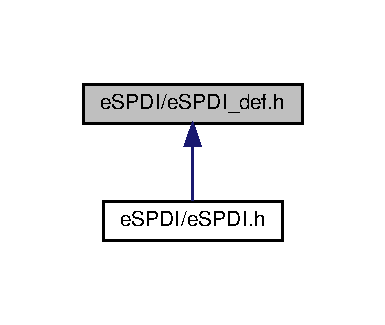
\includegraphics[width=185pt]{e_s_p_d_i__def_8h__dep__incl}
\end{center}
\end{figure}
\subsection*{Classes}
\begin{DoxyCompactItemize}
\item 
struct \hyperlink{structpacket__s}{packet\+\_\+s}
\item 
struct \hyperlink{structtag_d_e_v_i_n_f_o_r_m_a_t_i_o_n}{tag\+D\+E\+V\+I\+N\+F\+O\+R\+M\+A\+T\+I\+ON}
\item 
struct \hyperlink{structtag_d_e_v_s_e_l}{tag\+D\+E\+V\+S\+EL}
\item 
struct \hyperlink{structtag_a_p_c___s_t_r_e_a_m___i_n_f_o}{tag\+A\+P\+C\+\_\+\+S\+T\+R\+E\+A\+M\+\_\+\+I\+N\+FO}
\item 
struct \hyperlink{structtag_z_d_table_info}{tag\+Z\+D\+Table\+Info}
\item 
struct \hyperlink{structtag_k_e_e_p___d_a_t_a___c_t_r_l}{tag\+K\+E\+E\+P\+\_\+\+D\+A\+T\+A\+\_\+\+C\+T\+RL}
\item 
struct \hyperlink{structe_s_p_ctrl___rect_log_data}{e\+S\+P\+Ctrl\+\_\+\+Rect\+Log\+Data}
\item 
struct \hyperlink{struct_gyro_tag}{Gyro\+Tag}
\item 
struct \hyperlink{struct_acceleration_tag}{Acceleration\+Tag}
\item 
struct \hyperlink{struct_compass_tag}{Compass\+Tag}
\item 
struct \hyperlink{struct_e_y_s_d_image_type}{E\+Y\+S\+D\+Image\+Type}
\item 
struct \hyperlink{struct_point_cloud_info}{Point\+Cloud\+Info}
\end{DoxyCompactItemize}
\subsection*{Macros}
\begin{DoxyCompactItemize}
\item 
\mbox{\Hypertarget{e_s_p_d_i__def_8h_a7d9e1f98b376e5b9d518898f364fe352}\label{e_s_p_d_i__def_8h_a7d9e1f98b376e5b9d518898f364fe352}} 
\#define {\bfseries A\+P\+C\+\_\+\+OK}~0
\item 
\mbox{\Hypertarget{e_s_p_d_i__def_8h_a5e0e5b2fbc9366227b00146061bc5ce0}\label{e_s_p_d_i__def_8h_a5e0e5b2fbc9366227b00146061bc5ce0}} 
\#define {\bfseries A\+P\+C\+\_\+\+No\+Device}~-\/1
\item 
\mbox{\Hypertarget{e_s_p_d_i__def_8h_aef3c04e39f66bdce990d71a3c233ea15}\label{e_s_p_d_i__def_8h_aef3c04e39f66bdce990d71a3c233ea15}} 
\#define {\bfseries A\+P\+C\+\_\+\+Null\+Ptr}~-\/2
\item 
\mbox{\Hypertarget{e_s_p_d_i__def_8h_acebf50581d2477c315e64cccb9bfd3bb}\label{e_s_p_d_i__def_8h_acebf50581d2477c315e64cccb9bfd3bb}} 
\#define {\bfseries A\+P\+C\+\_\+\+Err\+Buf\+Len}~-\/3
\item 
\mbox{\Hypertarget{e_s_p_d_i__def_8h_a1e630175161853aa00f5cf577f225312}\label{e_s_p_d_i__def_8h_a1e630175161853aa00f5cf577f225312}} 
\#define {\bfseries A\+P\+C\+\_\+\+Init\+\_\+\+Fail}~-\/4
\item 
\mbox{\Hypertarget{e_s_p_d_i__def_8h_a062a6dfa94ac1a9710a6bfff5a3d92ad}\label{e_s_p_d_i__def_8h_a062a6dfa94ac1a9710a6bfff5a3d92ad}} 
\#define {\bfseries A\+P\+C\+\_\+\+No\+Z\+D\+Table}~-\/5
\item 
\mbox{\Hypertarget{e_s_p_d_i__def_8h_ace3257e26c5687dc17384864cfbae5c9}\label{e_s_p_d_i__def_8h_ace3257e26c5687dc17384864cfbae5c9}} 
\#define {\bfseries A\+P\+C\+\_\+\+R\+E\+A\+D\+F\+L\+A\+S\+H\+F\+A\+IL}~-\/6
\item 
\mbox{\Hypertarget{e_s_p_d_i__def_8h_adec309282f088b6097a62873b20c274e}\label{e_s_p_d_i__def_8h_adec309282f088b6097a62873b20c274e}} 
\#define {\bfseries A\+P\+C\+\_\+\+W\+R\+I\+T\+E\+F\+L\+A\+S\+H\+F\+A\+IL}~-\/7
\item 
\mbox{\Hypertarget{e_s_p_d_i__def_8h_a194c5c8f8e841f1d47e3ff2718f050b9}\label{e_s_p_d_i__def_8h_a194c5c8f8e841f1d47e3ff2718f050b9}} 
\#define {\bfseries A\+P\+C\+\_\+\+V\+E\+R\+I\+F\+Y\+\_\+\+D\+A\+T\+A\+\_\+\+F\+A\+IL}~-\/8
\item 
\mbox{\Hypertarget{e_s_p_d_i__def_8h_a8d8c6d48981186932b0415b42596f369}\label{e_s_p_d_i__def_8h_a8d8c6d48981186932b0415b42596f369}} 
\#define {\bfseries A\+P\+C\+\_\+\+K\+E\+E\+P\+\_\+\+D\+A\+T\+A\+\_\+\+F\+A\+IL}~-\/9
\item 
\mbox{\Hypertarget{e_s_p_d_i__def_8h_a1a9e1a453573616ccb59910d05b67ef3}\label{e_s_p_d_i__def_8h_a1a9e1a453573616ccb59910d05b67ef3}} 
\#define {\bfseries A\+P\+C\+\_\+\+R\+E\+C\+T\+\_\+\+D\+A\+T\+A\+\_\+\+L\+E\+N\+\_\+\+F\+A\+IL}~-\/10
\item 
\mbox{\Hypertarget{e_s_p_d_i__def_8h_a0ffb30fce538db2a70b37755a7e9a5b5}\label{e_s_p_d_i__def_8h_a0ffb30fce538db2a70b37755a7e9a5b5}} 
\#define {\bfseries A\+P\+C\+\_\+\+R\+E\+C\+T\+\_\+\+D\+A\+T\+A\+\_\+\+P\+A\+R\+S\+I\+N\+G\+\_\+\+F\+A\+IL}~-\/11
\item 
\mbox{\Hypertarget{e_s_p_d_i__def_8h_ad9f4f722d9168b43f2728e460a8c6fd7}\label{e_s_p_d_i__def_8h_ad9f4f722d9168b43f2728e460a8c6fd7}} 
\#define {\bfseries A\+P\+C\+\_\+\+R\+E\+T\+\_\+\+B\+A\+D\+\_\+\+P\+A\+R\+AM}~-\/12
\item 
\mbox{\Hypertarget{e_s_p_d_i__def_8h_a6cd4b773cae8cfbf94f2218b0c774589}\label{e_s_p_d_i__def_8h_a6cd4b773cae8cfbf94f2218b0c774589}} 
\#define {\bfseries A\+P\+C\+\_\+\+R\+E\+T\+\_\+\+O\+P\+E\+N\+\_\+\+F\+I\+L\+E\+\_\+\+F\+A\+IL}~-\/13
\item 
\mbox{\Hypertarget{e_s_p_d_i__def_8h_a999c9cc0db144cc017a19ef5da2d27db}\label{e_s_p_d_i__def_8h_a999c9cc0db144cc017a19ef5da2d27db}} 
\#define {\bfseries A\+P\+C\+\_\+\+N\+O\+\_\+\+C\+A\+L\+I\+B\+R\+A\+T\+I\+O\+N\+\_\+\+L\+OG}~-\/14
\item 
\mbox{\Hypertarget{e_s_p_d_i__def_8h_a778e6b36a9e716f9e3a5ae2103fb119f}\label{e_s_p_d_i__def_8h_a778e6b36a9e716f9e3a5ae2103fb119f}} 
\#define {\bfseries A\+P\+C\+\_\+\+P\+O\+S\+T\+P\+R\+O\+C\+E\+S\+S\+\_\+\+I\+N\+I\+T\+\_\+\+F\+A\+IL}~-\/15
\item 
\mbox{\Hypertarget{e_s_p_d_i__def_8h_a14e82e26d24ff8cda838b1aa463b1b13}\label{e_s_p_d_i__def_8h_a14e82e26d24ff8cda838b1aa463b1b13}} 
\#define {\bfseries A\+P\+C\+\_\+\+P\+O\+S\+T\+P\+R\+O\+C\+E\+S\+S\+\_\+\+N\+O\+T\+\_\+\+I\+N\+IT}~-\/16
\item 
\mbox{\Hypertarget{e_s_p_d_i__def_8h_adf9af36967836a366befe688f47d5c2a}\label{e_s_p_d_i__def_8h_adf9af36967836a366befe688f47d5c2a}} 
\#define {\bfseries A\+P\+C\+\_\+\+P\+O\+S\+T\+P\+R\+O\+C\+E\+S\+S\+\_\+\+F\+R\+A\+M\+E\+\_\+\+F\+A\+IL}~-\/17
\item 
\mbox{\Hypertarget{e_s_p_d_i__def_8h_a70dd5a7e245610735ba7072f334019e6}\label{e_s_p_d_i__def_8h_a70dd5a7e245610735ba7072f334019e6}} 
\#define {\bfseries A\+P\+C\+\_\+\+Not\+Support}~-\/18
\item 
\mbox{\Hypertarget{e_s_p_d_i__def_8h_aa7814df1d6efdfbe001e307c1dc65a13}\label{e_s_p_d_i__def_8h_aa7814df1d6efdfbe001e307c1dc65a13}} 
\#define {\bfseries A\+P\+C\+\_\+\+G\+E\+T\+\_\+\+R\+E\+S\+\_\+\+L\+I\+S\+T\+\_\+\+F\+A\+IL}~-\/19
\item 
\mbox{\Hypertarget{e_s_p_d_i__def_8h_a413b46ebe12c80a3b66a331d7e8a6ab0}\label{e_s_p_d_i__def_8h_a413b46ebe12c80a3b66a331d7e8a6ab0}} 
\#define {\bfseries A\+P\+C\+\_\+\+R\+E\+A\+D\+\_\+\+R\+E\+G\+\_\+\+F\+A\+IL}~-\/20
\item 
\mbox{\Hypertarget{e_s_p_d_i__def_8h_af99a9b7ca79c922a6ff20106404f9b4b}\label{e_s_p_d_i__def_8h_af99a9b7ca79c922a6ff20106404f9b4b}} 
\#define {\bfseries A\+P\+C\+\_\+\+W\+R\+I\+T\+E\+\_\+\+R\+E\+G\+\_\+\+F\+A\+IL}~-\/21
\item 
\mbox{\Hypertarget{e_s_p_d_i__def_8h_aab3a000d0ee47a66b4c271b6cdba0ad0}\label{e_s_p_d_i__def_8h_aab3a000d0ee47a66b4c271b6cdba0ad0}} 
\#define {\bfseries A\+P\+C\+\_\+\+S\+E\+T\+\_\+\+F\+P\+S\+\_\+\+F\+A\+IL}~-\/22
\item 
\mbox{\Hypertarget{e_s_p_d_i__def_8h_af7fefd080281392a63bb31374048d193}\label{e_s_p_d_i__def_8h_af7fefd080281392a63bb31374048d193}} 
\#define {\bfseries A\+P\+C\+\_\+\+V\+I\+D\+E\+O\+\_\+\+R\+E\+N\+D\+E\+R\+\_\+\+F\+A\+IL}~-\/23
\item 
\mbox{\Hypertarget{e_s_p_d_i__def_8h_ad16a017ec0eb6ecb10d1d044d7a5834c}\label{e_s_p_d_i__def_8h_ad16a017ec0eb6ecb10d1d044d7a5834c}} 
\#define {\bfseries A\+P\+C\+\_\+\+O\+P\+E\+N\+\_\+\+D\+E\+V\+I\+C\+E\+\_\+\+F\+A\+IL}~-\/24
\item 
\mbox{\Hypertarget{e_s_p_d_i__def_8h_a6881bc3d6a0bd5a47edca5d1e676f4b9}\label{e_s_p_d_i__def_8h_a6881bc3d6a0bd5a47edca5d1e676f4b9}} 
\#define {\bfseries A\+P\+C\+\_\+\+F\+I\+N\+D\+\_\+\+D\+E\+V\+I\+C\+E\+\_\+\+F\+A\+IL}~-\/25
\item 
\mbox{\Hypertarget{e_s_p_d_i__def_8h_a954ca15de82d114f96ce66e569dbbd7c}\label{e_s_p_d_i__def_8h_a954ca15de82d114f96ce66e569dbbd7c}} 
\#define {\bfseries A\+P\+C\+\_\+\+G\+E\+T\+\_\+\+I\+M\+A\+G\+E\+\_\+\+F\+A\+IL}~-\/26
\item 
\mbox{\Hypertarget{e_s_p_d_i__def_8h_a4419a27e71a568efcb067939de4545d3}\label{e_s_p_d_i__def_8h_a4419a27e71a568efcb067939de4545d3}} 
\#define {\bfseries A\+P\+C\+\_\+\+N\+O\+T\+\_\+\+S\+U\+P\+P\+O\+R\+T\+\_\+\+R\+ES}~-\/27
\item 
\mbox{\Hypertarget{e_s_p_d_i__def_8h_a3e3564214007ea84b73446dca968fbf5}\label{e_s_p_d_i__def_8h_a3e3564214007ea84b73446dca968fbf5}} 
\#define {\bfseries A\+P\+C\+\_\+\+C\+A\+L\+L\+B\+A\+C\+K\+\_\+\+R\+E\+G\+I\+S\+T\+E\+R\+\_\+\+F\+A\+IL}~-\/28
\item 
\mbox{\Hypertarget{e_s_p_d_i__def_8h_a6a1fe83867ba07ed079b2b16bf52a198}\label{e_s_p_d_i__def_8h_a6a1fe83867ba07ed079b2b16bf52a198}} 
\#define {\bfseries A\+P\+C\+\_\+\+C\+L\+O\+S\+E\+\_\+\+D\+E\+V\+I\+C\+E\+\_\+\+F\+A\+IL}~-\/29
\item 
\mbox{\Hypertarget{e_s_p_d_i__def_8h_ade7fd071db9a9b7cb1f38d4bcbdfaf10}\label{e_s_p_d_i__def_8h_ade7fd071db9a9b7cb1f38d4bcbdfaf10}} 
\#define {\bfseries A\+P\+C\+\_\+\+G\+E\+T\+\_\+\+C\+A\+L\+I\+B\+R\+A\+T\+I\+O\+N\+L\+O\+G\+\_\+\+F\+A\+IL}~-\/30
\item 
\mbox{\Hypertarget{e_s_p_d_i__def_8h_a694dc6937ca9991bea024b3ba5cfbbf5}\label{e_s_p_d_i__def_8h_a694dc6937ca9991bea024b3ba5cfbbf5}} 
\#define {\bfseries A\+P\+C\+\_\+\+S\+E\+T\+\_\+\+C\+A\+L\+I\+B\+R\+A\+T\+I\+O\+N\+L\+O\+G\+\_\+\+F\+A\+IL}~-\/31
\item 
\mbox{\Hypertarget{e_s_p_d_i__def_8h_aac77cad690dae97d92ce800430f6b117}\label{e_s_p_d_i__def_8h_aac77cad690dae97d92ce800430f6b117}} 
\#define {\bfseries A\+P\+C\+\_\+\+D\+E\+V\+I\+C\+E\+\_\+\+N\+O\+T\+\_\+\+S\+U\+P\+P\+O\+RT}~-\/32
\item 
\mbox{\Hypertarget{e_s_p_d_i__def_8h_aef4ebfa25f2335f0592aac28a7665680}\label{e_s_p_d_i__def_8h_aef4ebfa25f2335f0592aac28a7665680}} 
\#define {\bfseries A\+P\+C\+\_\+\+D\+E\+V\+I\+C\+E\+\_\+\+B\+U\+SY}~-\/33
\item 
\mbox{\Hypertarget{e_s_p_d_i__def_8h_a5d478e70ca1a16aafa595df93cd6dcc2}\label{e_s_p_d_i__def_8h_a5d478e70ca1a16aafa595df93cd6dcc2}} 
\#define {\bfseries A\+P\+C\+\_\+\+D\+E\+V\+I\+C\+E\+\_\+\+T\+I\+M\+E\+O\+UT}~-\/34
\item 
\mbox{\Hypertarget{e_s_p_d_i__def_8h_a1911f6432761e42a59a04d0fb257c61b}\label{e_s_p_d_i__def_8h_a1911f6432761e42a59a04d0fb257c61b}} 
\#define {\bfseries A\+P\+C\+\_\+\+I\+O\+\_\+\+S\+E\+L\+E\+C\+T\+\_\+\+E\+I\+N\+TR}~-\/35
\item 
\mbox{\Hypertarget{e_s_p_d_i__def_8h_a50555862fe7f869c6732b97970dbef7a}\label{e_s_p_d_i__def_8h_a50555862fe7f869c6732b97970dbef7a}} 
\#define {\bfseries A\+P\+C\+\_\+\+I\+O\+\_\+\+S\+E\+L\+E\+C\+T\+\_\+\+E\+R\+R\+OR}~-\/36
\item 
\mbox{\Hypertarget{e_s_p_d_i__def_8h_ac08704c358a64fad2aeb210572cd0a89}\label{e_s_p_d_i__def_8h_ac08704c358a64fad2aeb210572cd0a89}} 
\#define {\bfseries A\+P\+C\+\_\+\+I\+L\+L\+E\+G\+A\+L\+\_\+\+A\+N\+G\+LE}~-\/40
\item 
\mbox{\Hypertarget{e_s_p_d_i__def_8h_ad27f118e3e91e205f70eaf48e51eb53e}\label{e_s_p_d_i__def_8h_ad27f118e3e91e205f70eaf48e51eb53e}} 
\#define {\bfseries A\+P\+C\+\_\+\+I\+L\+L\+E\+G\+A\+L\+\_\+\+S\+T\+EP}~-\/41
\item 
\mbox{\Hypertarget{e_s_p_d_i__def_8h_a8555e8c3caeb109d412b651e608d4ddb}\label{e_s_p_d_i__def_8h_a8555e8c3caeb109d412b651e608d4ddb}} 
\#define {\bfseries A\+P\+C\+\_\+\+I\+L\+L\+E\+G\+A\+L\+\_\+\+T\+I\+M\+E\+P\+E\+R\+S\+T\+EP}~-\/42
\item 
\mbox{\Hypertarget{e_s_p_d_i__def_8h_a73a668ba12c75c15d3b0731082d4b5c5}\label{e_s_p_d_i__def_8h_a73a668ba12c75c15d3b0731082d4b5c5}} 
\#define {\bfseries A\+P\+C\+\_\+\+M\+O\+T\+O\+R\+\_\+\+R\+U\+N\+N\+I\+NG}~-\/43
\item 
\mbox{\Hypertarget{e_s_p_d_i__def_8h_a256dadb8ebd35a4a9c44abd8bf1bf4ba}\label{e_s_p_d_i__def_8h_a256dadb8ebd35a4a9c44abd8bf1bf4ba}} 
\#define {\bfseries A\+P\+C\+\_\+\+G\+E\+T\+S\+E\+N\+S\+O\+R\+R\+E\+G\+\_\+\+F\+A\+IL}~-\/44
\item 
\mbox{\Hypertarget{e_s_p_d_i__def_8h_a212928cde8e07882433c39f19b4f85ff}\label{e_s_p_d_i__def_8h_a212928cde8e07882433c39f19b4f85ff}} 
\#define {\bfseries A\+P\+C\+\_\+\+S\+E\+T\+S\+E\+N\+S\+O\+R\+R\+E\+G\+\_\+\+F\+A\+IL}~-\/45
\item 
\mbox{\Hypertarget{e_s_p_d_i__def_8h_aa893c59e03d1dbd2e34d068c6db47070}\label{e_s_p_d_i__def_8h_aa893c59e03d1dbd2e34d068c6db47070}} 
\#define {\bfseries A\+P\+C\+\_\+\+R\+E\+A\+D\+\_\+\+X\+\_\+\+A\+X\+I\+S\+\_\+\+F\+A\+IL}~-\/46
\item 
\mbox{\Hypertarget{e_s_p_d_i__def_8h_a19a645625a559aaa638bd16e38637fc5}\label{e_s_p_d_i__def_8h_a19a645625a559aaa638bd16e38637fc5}} 
\#define {\bfseries A\+P\+C\+\_\+\+R\+E\+A\+D\+\_\+\+Y\+\_\+\+A\+X\+I\+S\+\_\+\+F\+A\+IL}~-\/47
\item 
\mbox{\Hypertarget{e_s_p_d_i__def_8h_a313e4cb7e109ad1a6035c99e3ec803bb}\label{e_s_p_d_i__def_8h_a313e4cb7e109ad1a6035c99e3ec803bb}} 
\#define {\bfseries A\+P\+C\+\_\+\+R\+E\+A\+D\+\_\+\+Z\+\_\+\+A\+X\+I\+S\+\_\+\+F\+A\+IL}~-\/48
\item 
\mbox{\Hypertarget{e_s_p_d_i__def_8h_a2b57b3d2c8be37c5538dbe9ae79f6fef}\label{e_s_p_d_i__def_8h_a2b57b3d2c8be37c5538dbe9ae79f6fef}} 
\#define {\bfseries A\+P\+C\+\_\+\+R\+E\+A\+D\+\_\+\+P\+R\+E\+S\+S\+\_\+\+D\+A\+T\+A\+\_\+\+F\+A\+IL}~-\/49
\item 
\mbox{\Hypertarget{e_s_p_d_i__def_8h_a0bc2012918587b732de840a593893d75}\label{e_s_p_d_i__def_8h_a0bc2012918587b732de840a593893d75}} 
\#define {\bfseries A\+P\+C\+\_\+\+R\+E\+A\+D\+\_\+\+T\+E\+M\+P\+E\+R\+A\+T\+U\+R\+E\+\_\+\+F\+A\+IL}~-\/50
\item 
\mbox{\Hypertarget{e_s_p_d_i__def_8h_adcc82a714cba9efbe9271a10b537aad5}\label{e_s_p_d_i__def_8h_adcc82a714cba9efbe9271a10b537aad5}} 
\#define {\bfseries A\+P\+C\+\_\+\+R\+E\+T\+U\+R\+N\+H\+O\+M\+E\+\_\+\+R\+U\+N\+N\+I\+NG}~-\/51
\item 
\mbox{\Hypertarget{e_s_p_d_i__def_8h_a4ef9ab1e28383a08c5fb5549ee34222a}\label{e_s_p_d_i__def_8h_a4ef9ab1e28383a08c5fb5549ee34222a}} 
\#define {\bfseries A\+P\+C\+\_\+\+M\+O\+T\+O\+T\+S\+T\+O\+P\+\_\+\+B\+Y\+\_\+\+H\+O\+M\+E\+\_\+\+I\+N\+D\+EX}~-\/52
\item 
\mbox{\Hypertarget{e_s_p_d_i__def_8h_afccca0584456c0e1b2c7d4cbbf2e54b0}\label{e_s_p_d_i__def_8h_afccca0584456c0e1b2c7d4cbbf2e54b0}} 
\#define {\bfseries A\+P\+C\+\_\+\+M\+O\+T\+O\+T\+S\+T\+O\+P\+\_\+\+B\+Y\+\_\+\+P\+R\+O\+T\+E\+C\+T\+\_\+\+S\+C\+H\+E\+ME}~-\/53
\item 
\mbox{\Hypertarget{e_s_p_d_i__def_8h_afccc22932f1551e2ee50643d691292a5}\label{e_s_p_d_i__def_8h_afccc22932f1551e2ee50643d691292a5}} 
\#define {\bfseries A\+P\+C\+\_\+\+M\+O\+T\+O\+T\+S\+T\+O\+P\+\_\+\+B\+Y\+\_\+\+N\+O\+R\+M\+AL}~-\/54
\item 
\mbox{\Hypertarget{e_s_p_d_i__def_8h_a63c935163dd04d2f457eec8460e05f90}\label{e_s_p_d_i__def_8h_a63c935163dd04d2f457eec8460e05f90}} 
\#define {\bfseries A\+P\+C\+\_\+\+I\+L\+L\+E\+G\+A\+L\+\_\+\+F\+I\+R\+M\+W\+A\+R\+E\+\_\+\+V\+E\+R\+S\+I\+ON}~-\/55
\item 
\mbox{\Hypertarget{e_s_p_d_i__def_8h_a27456fd424f020f41881477539c9bf37}\label{e_s_p_d_i__def_8h_a27456fd424f020f41881477539c9bf37}} 
\#define {\bfseries A\+P\+C\+\_\+\+I\+L\+L\+E\+G\+A\+L\+\_\+\+S\+T\+E\+P\+P\+E\+R\+T\+I\+ME}~-\/56
\item 
\mbox{\Hypertarget{e_s_p_d_i__def_8h_a5d475f5f197c8d1b5c359606aeda0cc9}\label{e_s_p_d_i__def_8h_a5d475f5f197c8d1b5c359606aeda0cc9}} 
\#define {\bfseries A\+P\+C\+\_\+\+G\+E\+T\+\_\+\+P\+U\+\_\+\+P\+R\+O\+P\+\_\+\+V\+A\+L\+\_\+\+F\+A\+IL}~-\/60
\item 
\mbox{\Hypertarget{e_s_p_d_i__def_8h_a89536e60a04d951c2773eccb7e50c195}\label{e_s_p_d_i__def_8h_a89536e60a04d951c2773eccb7e50c195}} 
\#define {\bfseries A\+P\+C\+\_\+\+S\+E\+T\+\_\+\+P\+U\+\_\+\+P\+R\+O\+P\+\_\+\+V\+A\+L\+\_\+\+F\+A\+IL}~-\/61
\item 
\mbox{\Hypertarget{e_s_p_d_i__def_8h_acef14ef6d5123e0ee71516503b17821f}\label{e_s_p_d_i__def_8h_acef14ef6d5123e0ee71516503b17821f}} 
\#define {\bfseries A\+P\+C\+\_\+\+G\+E\+T\+\_\+\+C\+T\+\_\+\+P\+R\+O\+P\+\_\+\+V\+A\+L\+\_\+\+F\+A\+IL}~-\/62
\item 
\mbox{\Hypertarget{e_s_p_d_i__def_8h_a18bde616910e5f727fd9ecc8f34ec44e}\label{e_s_p_d_i__def_8h_a18bde616910e5f727fd9ecc8f34ec44e}} 
\#define {\bfseries A\+P\+C\+\_\+\+S\+E\+T\+\_\+\+C\+T\+\_\+\+P\+R\+O\+P\+\_\+\+V\+A\+L\+\_\+\+F\+A\+IL}~-\/63
\item 
\mbox{\Hypertarget{e_s_p_d_i__def_8h_aac267feb33ccc635e5c00b0f5d4af120}\label{e_s_p_d_i__def_8h_aac267feb33ccc635e5c00b0f5d4af120}} 
\#define {\bfseries A\+P\+C\+\_\+\+G\+E\+T\+\_\+\+C\+T\+\_\+\+P\+R\+O\+P\+\_\+\+R\+A\+N\+G\+E\+\_\+\+S\+T\+E\+P\+\_\+\+F\+A\+IL}~-\/64
\item 
\mbox{\Hypertarget{e_s_p_d_i__def_8h_a1037da23ba78a18dd57b44dc1cd0b992}\label{e_s_p_d_i__def_8h_a1037da23ba78a18dd57b44dc1cd0b992}} 
\#define {\bfseries A\+P\+C\+\_\+\+G\+E\+T\+\_\+\+P\+U\+\_\+\+P\+R\+O\+P\+\_\+\+R\+A\+N\+G\+E\+\_\+\+S\+T\+E\+P\+\_\+\+F\+A\+IL}~-\/65
\item 
\mbox{\Hypertarget{e_s_p_d_i__def_8h_a96d645aa015f50f3d3f6740eeac49ddd}\label{e_s_p_d_i__def_8h_a96d645aa015f50f3d3f6740eeac49ddd}} 
\#define {\bfseries A\+P\+C\+\_\+\+I\+N\+V\+A\+L\+I\+D\+\_\+\+U\+S\+E\+R\+D\+A\+TA}~-\/70
\item 
\mbox{\Hypertarget{e_s_p_d_i__def_8h_a0090e90f27a63af33cb3ed15e88f07f3}\label{e_s_p_d_i__def_8h_a0090e90f27a63af33cb3ed15e88f07f3}} 
\#define {\bfseries A\+P\+C\+\_\+\+M\+A\+P\+\_\+\+L\+U\+T\+\_\+\+F\+A\+IL}~-\/71
\item 
\mbox{\Hypertarget{e_s_p_d_i__def_8h_a8bcb8f7e772d38a80624407e5ad6f034}\label{e_s_p_d_i__def_8h_a8bcb8f7e772d38a80624407e5ad6f034}} 
\#define {\bfseries A\+P\+C\+\_\+\+A\+P\+P\+E\+N\+D\+\_\+\+T\+O\+\_\+\+F\+I\+L\+E\+\_\+\+F\+R\+O\+N\+T\+\_\+\+F\+A\+IL}~-\/72
\item 
\mbox{\Hypertarget{e_s_p_d_i__def_8h_a2f6b3db7d329e8a22bb5d6248a67a968}\label{e_s_p_d_i__def_8h_a2f6b3db7d329e8a22bb5d6248a67a968}} 
\#define {\bfseries A\+P\+C\+\_\+\+T\+O\+O\+\_\+\+M\+A\+N\+Y\+\_\+\+D\+E\+V\+I\+CE}~-\/80
\item 
\mbox{\Hypertarget{e_s_p_d_i__def_8h_a8deb3d69925c8275c9f49dc8251c8e34}\label{e_s_p_d_i__def_8h_a8deb3d69925c8275c9f49dc8251c8e34}} 
\#define {\bfseries A\+P\+C\+\_\+\+A\+C\+C\+E\+S\+S\+\_\+\+M\+P4\+\_\+\+E\+X\+T\+R\+A\+\_\+\+D\+A\+T\+A\+\_\+\+F\+A\+IL}~-\/81
\item 
\mbox{\Hypertarget{e_s_p_d_i__def_8h_ade3c083fa7b1178fcca5671e1830f2f9}\label{e_s_p_d_i__def_8h_ade3c083fa7b1178fcca5671e1830f2f9}} 
\#define {\bfseries B\+I\+T\+\_\+\+S\+ET}(a,  b)~((a) $\vert$= (1$<$$<$(b)))
\item 
\mbox{\Hypertarget{e_s_p_d_i__def_8h_a77fc3a931d1ad5fa08201e5c544817a0}\label{e_s_p_d_i__def_8h_a77fc3a931d1ad5fa08201e5c544817a0}} 
\#define {\bfseries B\+I\+T\+\_\+\+C\+L\+E\+AR}(a,  b)~((a) \&= $\sim$(1$<$$<$(b)))
\item 
\mbox{\Hypertarget{e_s_p_d_i__def_8h_ab6e0e32ff769c3cf2953456593e5663e}\label{e_s_p_d_i__def_8h_ab6e0e32ff769c3cf2953456593e5663e}} 
\#define {\bfseries B\+I\+T\+\_\+\+F\+L\+IP}(a,  b)~((a) $^\wedge$= (1$<$$<$(b)))
\item 
\mbox{\Hypertarget{e_s_p_d_i__def_8h_ab53403b709717305a8d0a8e692a70de6}\label{e_s_p_d_i__def_8h_ab53403b709717305a8d0a8e692a70de6}} 
\#define {\bfseries B\+I\+T\+\_\+\+C\+H\+E\+CK}(a,  b)~((a) \& (1$<$$<$(b)))
\item 
\mbox{\Hypertarget{e_s_p_d_i__def_8h_a23ec269c70f10e27159bb7c554a221ec}\label{e_s_p_d_i__def_8h_a23ec269c70f10e27159bb7c554a221ec}} 
\#define {\bfseries F\+G\+\_\+\+Address\+\_\+1\+Byte}~0x01
\item 
\mbox{\Hypertarget{e_s_p_d_i__def_8h_a7117ae8c720906fb5180bab6d701a3ca}\label{e_s_p_d_i__def_8h_a7117ae8c720906fb5180bab6d701a3ca}} 
\#define {\bfseries F\+G\+\_\+\+Address\+\_\+2\+Byte}~0x02
\item 
\mbox{\Hypertarget{e_s_p_d_i__def_8h_a00872efcb2b0081f9e81b05a63cac174}\label{e_s_p_d_i__def_8h_a00872efcb2b0081f9e81b05a63cac174}} 
\#define {\bfseries F\+G\+\_\+\+Value\+\_\+1\+Byte}~0x10
\item 
\mbox{\Hypertarget{e_s_p_d_i__def_8h_a1d44cb5cd0ec4a1434bcbfa250d7f385}\label{e_s_p_d_i__def_8h_a1d44cb5cd0ec4a1434bcbfa250d7f385}} 
\#define {\bfseries F\+G\+\_\+\+Value\+\_\+2\+Byte}~0x20
\item 
\mbox{\Hypertarget{e_s_p_d_i__def_8h_a82b2ac14aed05f228a3ce0f3d1491281}\label{e_s_p_d_i__def_8h_a82b2ac14aed05f228a3ce0f3d1491281}} 
\#define {\bfseries E\+V\+E\+N\+T\+\_\+\+B\+U\+F\+F\+E\+R\+\_\+\+S\+H\+M\+\_\+\+C\+O\+L\+OR}~\char`\"{}/shm\+\_\+ring\+\_\+buffer\+\_\+color\char`\"{}
\item 
\mbox{\Hypertarget{e_s_p_d_i__def_8h_a135177a342f1b6f8937a050486149f8a}\label{e_s_p_d_i__def_8h_a135177a342f1b6f8937a050486149f8a}} 
\#define {\bfseries E\+V\+E\+N\+T\+\_\+\+B\+U\+F\+F\+E\+R\+\_\+\+S\+H\+M\+\_\+\+D\+E\+P\+TH}~\char`\"{}/shm\+\_\+ring\+\_\+buffer\+\_\+depth\char`\"{}
\item 
\mbox{\Hypertarget{e_s_p_d_i__def_8h_aaaf37b51b6c10820b69d75dbf529d23a}\label{e_s_p_d_i__def_8h_aaaf37b51b6c10820b69d75dbf529d23a}} 
\#define {\bfseries E\+V\+E\+N\+T\+\_\+\+B\+U\+F\+F\+E\+R\+\_\+\+S\+HM}~\char`\"{}/shm\+\_\+ring\+\_\+buffer\char`\"{}
\item 
\mbox{\Hypertarget{e_s_p_d_i__def_8h_a0377a140d04bf55825e96d65ce8665aa}\label{e_s_p_d_i__def_8h_a0377a140d04bf55825e96d65ce8665aa}} 
\#define {\bfseries C\+M\+D\+\_\+\+F\+I\+F\+O\+\_\+\+P\+A\+TH}~\char`\"{}/tmp/cmdfifo\char`\"{}
\item 
\mbox{\Hypertarget{e_s_p_d_i__def_8h_aa270af458a4e54eca0cf5cb8e19f217b}\label{e_s_p_d_i__def_8h_aa270af458a4e54eca0cf5cb8e19f217b}} 
\#define {\bfseries Z\+D\+\_\+\+P\+A\+TH}~\char`\"{}/tmp/zd\+\_\+addr\char`\"{}
\item 
\mbox{\Hypertarget{e_s_p_d_i__def_8h_a61471b3fa90d6002fba297831f0d9d8c}\label{e_s_p_d_i__def_8h_a61471b3fa90d6002fba297831f0d9d8c}} 
\#define {\bfseries R\+E\+C\+T\+I\+F\+Y\+\_\+\+L\+O\+G\+\_\+\+P\+A\+TH}~\char`\"{}/tmp/rectifylog\+\_\+addr\char`\"{}
\item 
\mbox{\Hypertarget{e_s_p_d_i__def_8h_a87af0ea87d146a7239f237b681698cec}\label{e_s_p_d_i__def_8h_a87af0ea87d146a7239f237b681698cec}} 
\#define {\bfseries S\+R\+B\+\_\+\+L\+E\+N\+G\+TH}~10
\item 
\mbox{\Hypertarget{e_s_p_d_i__def_8h_a25a6b2f06a96e55942a022b80d8a96da}\label{e_s_p_d_i__def_8h_a25a6b2f06a96e55942a022b80d8a96da}} 
\#define {\bfseries C\+H\+I\+P\+I\+D\+\_\+\+A\+D\+DR}~0xf014
\item 
\mbox{\Hypertarget{e_s_p_d_i__def_8h_a6e8ac08f548d7275317079e92f9d08ed}\label{e_s_p_d_i__def_8h_a6e8ac08f548d7275317079e92f9d08ed}} 
\#define {\bfseries S\+E\+R\+I\+A\+L\+\_\+2\+B\+I\+T\+\_\+\+A\+D\+DR}~0xf0fe
\item 
\mbox{\Hypertarget{e_s_p_d_i__def_8h_ae7b7511b0dd516ed720bd5183a224ebb}\label{e_s_p_d_i__def_8h_ae7b7511b0dd516ed720bd5183a224ebb}} 
\#define {\bfseries A\+P\+C\+\_\+\+D\+E\+P\+T\+H\+\_\+\+D\+A\+T\+A\+\_\+\+O\+F\+F\+\_\+\+R\+AW}~0 /$\ast$ raw (depth off, only raw color) $\ast$/
\item 
\mbox{\Hypertarget{e_s_p_d_i__def_8h_a4ad860115f7aef5301fc5afbf8b07b99}\label{e_s_p_d_i__def_8h_a4ad860115f7aef5301fc5afbf8b07b99}} 
\#define {\bfseries A\+P\+C\+\_\+\+D\+E\+P\+T\+H\+\_\+\+D\+A\+T\+A\+\_\+\+D\+E\+F\+A\+U\+LT}~0 /$\ast$ raw (depth off, only raw color) $\ast$/
\item 
\mbox{\Hypertarget{e_s_p_d_i__def_8h_ad9050f5766cc513741f2b823ed0a0c86}\label{e_s_p_d_i__def_8h_ad9050f5766cc513741f2b823ed0a0c86}} 
\#define {\bfseries A\+P\+C\+\_\+\+D\+E\+P\+T\+H\+\_\+\+D\+A\+T\+A\+\_\+8\+\_\+\+B\+I\+TS}~1 /$\ast$ rectify, 1 byte per pixel $\ast$/
\item 
\mbox{\Hypertarget{e_s_p_d_i__def_8h_a16c7dea3f16e2e113e71123b317b11d5}\label{e_s_p_d_i__def_8h_a16c7dea3f16e2e113e71123b317b11d5}} 
\#define {\bfseries A\+P\+C\+\_\+\+D\+E\+P\+T\+H\+\_\+\+D\+A\+T\+A\+\_\+14\+\_\+\+B\+I\+TS}~2 /$\ast$ rectify, 2 byte per pixel $\ast$/
\item 
\mbox{\Hypertarget{e_s_p_d_i__def_8h_ad513af8ac7a14e33ec8e6949dbc85005}\label{e_s_p_d_i__def_8h_ad513af8ac7a14e33ec8e6949dbc85005}} 
\#define {\bfseries A\+P\+C\+\_\+\+D\+E\+P\+T\+H\+\_\+\+D\+A\+T\+A\+\_\+8\+\_\+\+B\+I\+T\+S\+\_\+x80}~3 /$\ast$ rectify, 2 byte per pixel but using 1 byte only $\ast$/
\item 
\mbox{\Hypertarget{e_s_p_d_i__def_8h_a5864e0e1fa39752a6d972b786dabd39b}\label{e_s_p_d_i__def_8h_a5864e0e1fa39752a6d972b786dabd39b}} 
\#define {\bfseries A\+P\+C\+\_\+\+D\+E\+P\+T\+H\+\_\+\+D\+A\+T\+A\+\_\+11\+\_\+\+B\+I\+TS}~4 /$\ast$ rectify, 2 byte per pixel but using 11 bit only $\ast$/
\item 
\mbox{\Hypertarget{e_s_p_d_i__def_8h_ae4a666269e61028fa2e9b6597a0b3996}\label{e_s_p_d_i__def_8h_ae4a666269e61028fa2e9b6597a0b3996}} 
\#define {\bfseries A\+P\+C\+\_\+\+D\+E\+P\+T\+H\+\_\+\+D\+A\+T\+A\+\_\+\+O\+F\+F\+\_\+\+R\+E\+C\+T\+I\+FY}~5 /$\ast$ rectify (depth off, only rectify color) $\ast$/
\item 
\mbox{\Hypertarget{e_s_p_d_i__def_8h_a7903a51d1f5028848b2c5c3222ceb170}\label{e_s_p_d_i__def_8h_a7903a51d1f5028848b2c5c3222ceb170}} 
\#define {\bfseries A\+P\+C\+\_\+\+D\+E\+P\+T\+H\+\_\+\+D\+A\+T\+A\+\_\+8\+\_\+\+B\+I\+T\+S\+\_\+\+R\+AW}~6 /$\ast$ raw $\ast$/
\item 
\mbox{\Hypertarget{e_s_p_d_i__def_8h_a9d8fd0c3a12a7df4c4461f6384f2d47e}\label{e_s_p_d_i__def_8h_a9d8fd0c3a12a7df4c4461f6384f2d47e}} 
\#define {\bfseries A\+P\+C\+\_\+\+D\+E\+P\+T\+H\+\_\+\+D\+A\+T\+A\+\_\+14\+\_\+\+B\+I\+T\+S\+\_\+\+R\+AW}~7 /$\ast$ raw $\ast$/
\item 
\mbox{\Hypertarget{e_s_p_d_i__def_8h_a1b861f91f472710f4712bb354cb61408}\label{e_s_p_d_i__def_8h_a1b861f91f472710f4712bb354cb61408}} 
\#define {\bfseries A\+P\+C\+\_\+\+D\+E\+P\+T\+H\+\_\+\+D\+A\+T\+A\+\_\+8\+\_\+\+B\+I\+T\+S\+\_\+x80\+\_\+\+R\+AW}~8 /$\ast$ raw $\ast$/
\item 
\mbox{\Hypertarget{e_s_p_d_i__def_8h_ace7d902703dc28faff7f79ac8b57a02c}\label{e_s_p_d_i__def_8h_ace7d902703dc28faff7f79ac8b57a02c}} 
\#define {\bfseries A\+P\+C\+\_\+\+D\+E\+P\+T\+H\+\_\+\+D\+A\+T\+A\+\_\+11\+\_\+\+B\+I\+T\+S\+\_\+\+R\+AW}~9 /$\ast$ raw $\ast$/
\item 
\mbox{\Hypertarget{e_s_p_d_i__def_8h_a909d66033a1bec875a9e1f0f1aa7452c}\label{e_s_p_d_i__def_8h_a909d66033a1bec875a9e1f0f1aa7452c}} 
\#define {\bfseries A\+P\+C\+\_\+\+D\+E\+P\+T\+H\+\_\+\+D\+A\+T\+A\+\_\+14\+\_\+\+B\+I\+T\+S\+\_\+\+C\+O\+M\+B\+I\+N\+E\+D\+\_\+\+R\+E\+C\+T\+I\+FY}~11
\item 
\mbox{\Hypertarget{e_s_p_d_i__def_8h_a63031ea0290867cb43d0943a80da151d}\label{e_s_p_d_i__def_8h_a63031ea0290867cb43d0943a80da151d}} 
\#define {\bfseries A\+P\+C\+\_\+\+D\+E\+P\+T\+H\+\_\+\+D\+A\+T\+A\+\_\+11\+\_\+\+B\+I\+T\+S\+\_\+\+C\+O\+M\+B\+I\+N\+E\+D\+\_\+\+R\+E\+C\+T\+I\+FY}~13
\item 
\mbox{\Hypertarget{e_s_p_d_i__def_8h_a8477961bb5002d548d3792ee107b3231}\label{e_s_p_d_i__def_8h_a8477961bb5002d548d3792ee107b3231}} 
\#define {\bfseries A\+P\+C\+\_\+\+D\+E\+P\+T\+H\+\_\+\+D\+A\+T\+A\+\_\+\+I\+N\+T\+E\+R\+L\+E\+A\+V\+E\+\_\+\+M\+O\+D\+E\+\_\+\+O\+F\+F\+S\+ET}~16
\item 
\mbox{\Hypertarget{e_s_p_d_i__def_8h_ab73623871a7017b9e8dc4d3d9440f3f0}\label{e_s_p_d_i__def_8h_ab73623871a7017b9e8dc4d3d9440f3f0}} 
\#define {\bfseries A\+P\+C\+\_\+\+D\+E\+P\+T\+H\+\_\+\+D\+A\+T\+A\+\_\+\+I\+L\+M\+\_\+\+O\+F\+F\+\_\+\+R\+AW}~A\+P\+C\+\_\+\+D\+E\+P\+T\+H\+\_\+\+D\+A\+T\+A\+\_\+\+O\+F\+F\+\_\+\+R\+AW + A\+P\+C\+\_\+\+D\+E\+P\+T\+H\+\_\+\+D\+A\+T\+A\+\_\+\+I\+N\+T\+E\+R\+L\+E\+A\+V\+E\+\_\+\+M\+O\+D\+E\+\_\+\+O\+F\+F\+S\+ET /$\ast$ raw (depth off, only raw color) $\ast$/
\item 
\mbox{\Hypertarget{e_s_p_d_i__def_8h_afc66bd89a930c612104b89b166c5c4d0}\label{e_s_p_d_i__def_8h_afc66bd89a930c612104b89b166c5c4d0}} 
\#define {\bfseries A\+P\+C\+\_\+\+D\+E\+P\+T\+H\+\_\+\+D\+A\+T\+A\+\_\+\+I\+L\+M\+\_\+\+D\+E\+F\+A\+U\+LT}~A\+P\+C\+\_\+\+D\+E\+P\+T\+H\+\_\+\+D\+A\+T\+A\+\_\+\+D\+E\+F\+A\+U\+LT + A\+P\+C\+\_\+\+D\+E\+P\+T\+H\+\_\+\+D\+A\+T\+A\+\_\+\+I\+N\+T\+E\+R\+L\+E\+A\+V\+E\+\_\+\+M\+O\+D\+E\+\_\+\+O\+F\+F\+S\+ET /$\ast$ raw (depth off, only raw color) $\ast$/
\item 
\mbox{\Hypertarget{e_s_p_d_i__def_8h_a0131412e89e4035c604c705b20ad94a0}\label{e_s_p_d_i__def_8h_a0131412e89e4035c604c705b20ad94a0}} 
\#define {\bfseries A\+P\+C\+\_\+\+D\+E\+P\+T\+H\+\_\+\+D\+A\+T\+A\+\_\+\+I\+L\+M\+\_\+8\+\_\+\+B\+I\+TS}~A\+P\+C\+\_\+\+D\+E\+P\+T\+H\+\_\+\+D\+A\+T\+A\+\_\+8\+\_\+\+B\+I\+TS + A\+P\+C\+\_\+\+D\+E\+P\+T\+H\+\_\+\+D\+A\+T\+A\+\_\+\+I\+N\+T\+E\+R\+L\+E\+A\+V\+E\+\_\+\+M\+O\+D\+E\+\_\+\+O\+F\+F\+S\+ET /$\ast$ rectify, 1 byte per pixel $\ast$/
\item 
\mbox{\Hypertarget{e_s_p_d_i__def_8h_ac2a91c2d60fd8c327aaa209a2c68a362}\label{e_s_p_d_i__def_8h_ac2a91c2d60fd8c327aaa209a2c68a362}} 
\#define {\bfseries A\+P\+C\+\_\+\+D\+E\+P\+T\+H\+\_\+\+D\+A\+T\+A\+\_\+\+I\+L\+M\+\_\+14\+\_\+\+B\+I\+TS}~A\+P\+C\+\_\+\+D\+E\+P\+T\+H\+\_\+\+D\+A\+T\+A\+\_\+14\+\_\+\+B\+I\+TS + A\+P\+C\+\_\+\+D\+E\+P\+T\+H\+\_\+\+D\+A\+T\+A\+\_\+\+I\+N\+T\+E\+R\+L\+E\+A\+V\+E\+\_\+\+M\+O\+D\+E\+\_\+\+O\+F\+F\+S\+ET /$\ast$ rectify, 2 byte per pixel $\ast$/
\item 
\mbox{\Hypertarget{e_s_p_d_i__def_8h_ac1300da9557a373a9a77809721bb735a}\label{e_s_p_d_i__def_8h_ac1300da9557a373a9a77809721bb735a}} 
\#define {\bfseries A\+P\+C\+\_\+\+D\+E\+P\+T\+H\+\_\+\+D\+A\+T\+A\+\_\+\+I\+L\+M\+\_\+8\+\_\+\+B\+I\+T\+S\+\_\+x80}~A\+P\+C\+\_\+\+D\+E\+P\+T\+H\+\_\+\+D\+A\+T\+A\+\_\+8\+\_\+\+B\+I\+T\+S\+\_\+x80 + A\+P\+C\+\_\+\+D\+E\+P\+T\+H\+\_\+\+D\+A\+T\+A\+\_\+\+I\+N\+T\+E\+R\+L\+E\+A\+V\+E\+\_\+\+M\+O\+D\+E\+\_\+\+O\+F\+F\+S\+ET /$\ast$ rectify, 2 byte per pixel but using 1 byte only $\ast$/
\item 
\mbox{\Hypertarget{e_s_p_d_i__def_8h_abed6609563f6caf14dc621d8a1415541}\label{e_s_p_d_i__def_8h_abed6609563f6caf14dc621d8a1415541}} 
\#define {\bfseries A\+P\+C\+\_\+\+D\+E\+P\+T\+H\+\_\+\+D\+A\+T\+A\+\_\+\+I\+L\+M\+\_\+11\+\_\+\+B\+I\+TS}~A\+P\+C\+\_\+\+D\+E\+P\+T\+H\+\_\+\+D\+A\+T\+A\+\_\+11\+\_\+\+B\+I\+TS + A\+P\+C\+\_\+\+D\+E\+P\+T\+H\+\_\+\+D\+A\+T\+A\+\_\+\+I\+N\+T\+E\+R\+L\+E\+A\+V\+E\+\_\+\+M\+O\+D\+E\+\_\+\+O\+F\+F\+S\+ET /$\ast$ rectify, 2 byte per pixel but using 11 bit only $\ast$/
\item 
\mbox{\Hypertarget{e_s_p_d_i__def_8h_a5afdab48b90f84dc81082e58c97fc73f}\label{e_s_p_d_i__def_8h_a5afdab48b90f84dc81082e58c97fc73f}} 
\#define {\bfseries A\+P\+C\+\_\+\+D\+E\+P\+T\+H\+\_\+\+D\+A\+T\+A\+\_\+\+I\+L\+M\+\_\+\+O\+F\+F\+\_\+\+R\+E\+C\+T\+I\+FY}~A\+P\+C\+\_\+\+D\+E\+P\+T\+H\+\_\+\+D\+A\+T\+A\+\_\+\+O\+F\+F\+\_\+\+R\+E\+C\+T\+I\+FY + A\+P\+C\+\_\+\+D\+E\+P\+T\+H\+\_\+\+D\+A\+T\+A\+\_\+\+I\+N\+T\+E\+R\+L\+E\+A\+V\+E\+\_\+\+M\+O\+D\+E\+\_\+\+O\+F\+F\+S\+ET /$\ast$ rectify (depth off, only rectify color) $\ast$/
\item 
\mbox{\Hypertarget{e_s_p_d_i__def_8h_a29ee6f9a9dc387e4f221fd05a72703f3}\label{e_s_p_d_i__def_8h_a29ee6f9a9dc387e4f221fd05a72703f3}} 
\#define {\bfseries A\+P\+C\+\_\+\+D\+E\+P\+T\+H\+\_\+\+D\+A\+T\+A\+\_\+\+I\+L\+M\+\_\+8\+\_\+\+B\+I\+T\+S\+\_\+\+R\+AW}~A\+P\+C\+\_\+\+D\+E\+P\+T\+H\+\_\+\+D\+A\+T\+A\+\_\+8\+\_\+\+B\+I\+T\+S\+\_\+\+R\+AW + A\+P\+C\+\_\+\+D\+E\+P\+T\+H\+\_\+\+D\+A\+T\+A\+\_\+\+I\+N\+T\+E\+R\+L\+E\+A\+V\+E\+\_\+\+M\+O\+D\+E\+\_\+\+O\+F\+F\+S\+ET /$\ast$ raw $\ast$/
\item 
\mbox{\Hypertarget{e_s_p_d_i__def_8h_a026bee54125af34cf9f9d754ee999854}\label{e_s_p_d_i__def_8h_a026bee54125af34cf9f9d754ee999854}} 
\#define {\bfseries A\+P\+C\+\_\+\+D\+E\+P\+T\+H\+\_\+\+D\+A\+T\+A\+\_\+\+I\+L\+M\+\_\+14\+\_\+\+B\+I\+T\+S\+\_\+\+R\+AW}~A\+P\+C\+\_\+\+D\+E\+P\+T\+H\+\_\+\+D\+A\+T\+A\+\_\+14\+\_\+\+B\+I\+T\+S\+\_\+\+R\+AW + A\+P\+C\+\_\+\+D\+E\+P\+T\+H\+\_\+\+D\+A\+T\+A\+\_\+\+I\+N\+T\+E\+R\+L\+E\+A\+V\+E\+\_\+\+M\+O\+D\+E\+\_\+\+O\+F\+F\+S\+ET /$\ast$ raw $\ast$/
\item 
\mbox{\Hypertarget{e_s_p_d_i__def_8h_a9e31fb5502b8737ca48e8990ebfb4f22}\label{e_s_p_d_i__def_8h_a9e31fb5502b8737ca48e8990ebfb4f22}} 
\#define {\bfseries A\+P\+C\+\_\+\+D\+E\+P\+T\+H\+\_\+\+D\+A\+T\+A\+\_\+\+I\+L\+M\+\_\+8\+\_\+\+B\+I\+T\+S\+\_\+x80\+\_\+\+R\+AW}~A\+P\+C\+\_\+\+D\+E\+P\+T\+H\+\_\+\+D\+A\+T\+A\+\_\+8\+\_\+\+B\+I\+T\+S\+\_\+x80\+\_\+\+R\+AW + A\+P\+C\+\_\+\+D\+E\+P\+T\+H\+\_\+\+D\+A\+T\+A\+\_\+\+I\+N\+T\+E\+R\+L\+E\+A\+V\+E\+\_\+\+M\+O\+D\+E\+\_\+\+O\+F\+F\+S\+ET /$\ast$ raw $\ast$/
\item 
\mbox{\Hypertarget{e_s_p_d_i__def_8h_a98f3471d4d4d1608772299d9ed959bcc}\label{e_s_p_d_i__def_8h_a98f3471d4d4d1608772299d9ed959bcc}} 
\#define {\bfseries A\+P\+C\+\_\+\+D\+E\+P\+T\+H\+\_\+\+D\+A\+T\+A\+\_\+\+I\+L\+M\+\_\+11\+\_\+\+B\+I\+T\+S\+\_\+\+R\+AW}~A\+P\+C\+\_\+\+D\+E\+P\+T\+H\+\_\+\+D\+A\+T\+A\+\_\+11\+\_\+\+B\+I\+T\+S\+\_\+\+R\+AW + A\+P\+C\+\_\+\+D\+E\+P\+T\+H\+\_\+\+D\+A\+T\+A\+\_\+\+I\+N\+T\+E\+R\+L\+E\+A\+V\+E\+\_\+\+M\+O\+D\+E\+\_\+\+O\+F\+F\+S\+ET /$\ast$ raw $\ast$/
\item 
\mbox{\Hypertarget{e_s_p_d_i__def_8h_aa2f229ceabd96bb6c10cab54ef1465f2}\label{e_s_p_d_i__def_8h_aa2f229ceabd96bb6c10cab54ef1465f2}} 
\#define {\bfseries A\+P\+C\+\_\+\+D\+E\+P\+T\+H\+\_\+\+D\+A\+T\+A\+\_\+\+I\+L\+M\+\_\+14\+\_\+\+B\+I\+T\+S\+\_\+\+C\+O\+M\+B\+I\+N\+E\+D\+\_\+\+R\+E\+C\+T\+I\+FY}~A\+P\+C\+\_\+\+D\+E\+P\+T\+H\+\_\+\+D\+A\+T\+A\+\_\+14\+\_\+\+B\+I\+T\+S\+\_\+\+C\+O\+M\+B\+I\+N\+E\+D\+\_\+\+R\+E\+C\+T\+I\+FY + A\+P\+C\+\_\+\+D\+E\+P\+T\+H\+\_\+\+D\+A\+T\+A\+\_\+\+I\+N\+T\+E\+R\+L\+E\+A\+V\+E\+\_\+\+M\+O\+D\+E\+\_\+\+O\+F\+F\+S\+ET
\item 
\mbox{\Hypertarget{e_s_p_d_i__def_8h_af73ea1817a35696064a8d30254057539}\label{e_s_p_d_i__def_8h_af73ea1817a35696064a8d30254057539}} 
\#define {\bfseries A\+P\+C\+\_\+\+D\+E\+P\+T\+H\+\_\+\+D\+A\+T\+A\+\_\+\+I\+L\+M\+\_\+11\+\_\+\+B\+I\+T\+S\+\_\+\+C\+O\+M\+B\+I\+N\+E\+D\+\_\+\+R\+E\+C\+T\+I\+FY}~A\+P\+C\+\_\+\+D\+E\+P\+T\+H\+\_\+\+D\+A\+T\+A\+\_\+11\+\_\+\+B\+I\+T\+S\+\_\+\+C\+O\+M\+B\+I\+N\+E\+D\+\_\+\+R\+E\+C\+T\+I\+FY + A\+P\+C\+\_\+\+D\+E\+P\+T\+H\+\_\+\+D\+A\+T\+A\+\_\+\+I\+N\+T\+E\+R\+L\+E\+A\+V\+E\+\_\+\+M\+O\+D\+E\+\_\+\+O\+F\+F\+S\+ET
\item 
\mbox{\Hypertarget{e_s_p_d_i__def_8h_a196883665783aaf9a2099c2c3f639613}\label{e_s_p_d_i__def_8h_a196883665783aaf9a2099c2c3f639613}} 
\#define {\bfseries A\+P\+C\+\_\+\+D\+E\+P\+T\+H\+\_\+\+D\+A\+T\+A\+\_\+\+S\+C\+A\+L\+E\+\_\+\+D\+O\+W\+N\+\_\+\+M\+O\+D\+E\+\_\+\+O\+F\+F\+S\+ET}~32
\item 
\mbox{\Hypertarget{e_s_p_d_i__def_8h_a91d4453a59bd2bc9cba0604352e12174}\label{e_s_p_d_i__def_8h_a91d4453a59bd2bc9cba0604352e12174}} 
\#define {\bfseries A\+P\+C\+\_\+\+D\+E\+P\+T\+H\+\_\+\+D\+A\+T\+A\+\_\+\+S\+C\+A\+L\+E\+\_\+\+D\+O\+W\+N\+\_\+\+O\+F\+F\+\_\+\+R\+AW}~(A\+P\+C\+\_\+\+D\+E\+P\+T\+H\+\_\+\+D\+A\+T\+A\+\_\+\+O\+F\+F\+\_\+\+R\+AW + A\+P\+C\+\_\+\+D\+E\+P\+T\+H\+\_\+\+D\+A\+T\+A\+\_\+\+S\+C\+A\+L\+E\+\_\+\+D\+O\+W\+N\+\_\+\+M\+O\+D\+E\+\_\+\+O\+F\+F\+S\+ET)/$\ast$ raw (depth off, only raw color) $\ast$/
\item 
\mbox{\Hypertarget{e_s_p_d_i__def_8h_ac9938ac31012cdefecfab8cc856c04f4}\label{e_s_p_d_i__def_8h_ac9938ac31012cdefecfab8cc856c04f4}} 
\#define {\bfseries A\+P\+C\+\_\+\+D\+E\+P\+T\+H\+\_\+\+D\+A\+T\+A\+\_\+\+S\+C\+A\+L\+E\+\_\+\+D\+O\+W\+N\+\_\+\+D\+E\+F\+A\+U\+LT}~(A\+P\+C\+\_\+\+D\+E\+P\+T\+H\+\_\+\+D\+A\+T\+A\+\_\+\+D\+E\+F\+A\+U\+LT + A\+P\+C\+\_\+\+D\+E\+P\+T\+H\+\_\+\+D\+A\+T\+A\+\_\+\+S\+C\+A\+L\+E\+\_\+\+D\+O\+W\+N\+\_\+\+M\+O\+D\+E\+\_\+\+O\+F\+F\+S\+ET)  /$\ast$ raw (depth off, only raw color) $\ast$/
\item 
\mbox{\Hypertarget{e_s_p_d_i__def_8h_a996054d647136b21a5ddace16d7b230e}\label{e_s_p_d_i__def_8h_a996054d647136b21a5ddace16d7b230e}} 
\#define {\bfseries A\+P\+C\+\_\+\+D\+E\+P\+T\+H\+\_\+\+D\+A\+T\+A\+\_\+\+S\+C\+A\+L\+E\+\_\+\+D\+O\+W\+N\+\_\+8\+\_\+\+B\+I\+TS}~(A\+P\+C\+\_\+\+D\+E\+P\+T\+H\+\_\+\+D\+A\+T\+A\+\_\+8\+\_\+\+B\+I\+TS + A\+P\+C\+\_\+\+D\+E\+P\+T\+H\+\_\+\+D\+A\+T\+A\+\_\+\+S\+C\+A\+L\+E\+\_\+\+D\+O\+W\+N\+\_\+\+M\+O\+D\+E\+\_\+\+O\+F\+F\+S\+ET)/$\ast$ rectify, 1 byte per pixel $\ast$/
\item 
\mbox{\Hypertarget{e_s_p_d_i__def_8h_a7ccf6e0d4c9fcea1dfa984487036e2c3}\label{e_s_p_d_i__def_8h_a7ccf6e0d4c9fcea1dfa984487036e2c3}} 
\#define {\bfseries A\+P\+C\+\_\+\+D\+E\+P\+T\+H\+\_\+\+D\+A\+T\+A\+\_\+\+S\+C\+A\+L\+E\+\_\+\+D\+O\+W\+N\+\_\+14\+\_\+\+B\+I\+TS}~(A\+P\+C\+\_\+\+D\+E\+P\+T\+H\+\_\+\+D\+A\+T\+A\+\_\+14\+\_\+\+B\+I\+TS + A\+P\+C\+\_\+\+D\+E\+P\+T\+H\+\_\+\+D\+A\+T\+A\+\_\+\+S\+C\+A\+L\+E\+\_\+\+D\+O\+W\+N\+\_\+\+M\+O\+D\+E\+\_\+\+O\+F\+F\+S\+ET) /$\ast$ rectify, 2 byte per pixel $\ast$/
\item 
\mbox{\Hypertarget{e_s_p_d_i__def_8h_a2275c882d4dcff8e73e3ad4f6b8fa015}\label{e_s_p_d_i__def_8h_a2275c882d4dcff8e73e3ad4f6b8fa015}} 
\#define {\bfseries A\+P\+C\+\_\+\+D\+E\+P\+T\+H\+\_\+\+D\+A\+T\+A\+\_\+\+S\+C\+A\+L\+E\+\_\+\+D\+O\+W\+N\+\_\+8\+\_\+\+B\+I\+T\+S\+\_\+x80}~(A\+P\+C\+\_\+\+D\+E\+P\+T\+H\+\_\+\+D\+A\+T\+A\+\_\+8\+\_\+\+B\+I\+T\+S\+\_\+x80 + A\+P\+C\+\_\+\+D\+E\+P\+T\+H\+\_\+\+D\+A\+T\+A\+\_\+\+S\+C\+A\+L\+E\+\_\+\+D\+O\+W\+N\+\_\+\+M\+O\+D\+E\+\_\+\+O\+F\+F\+S\+ET) /$\ast$ rectify, 2 byte per pixel but using 1 byte only $\ast$/
\item 
\mbox{\Hypertarget{e_s_p_d_i__def_8h_a87f5eb9a658548ad3aca512b81ac4c4f}\label{e_s_p_d_i__def_8h_a87f5eb9a658548ad3aca512b81ac4c4f}} 
\#define {\bfseries A\+P\+C\+\_\+\+D\+E\+P\+T\+H\+\_\+\+D\+A\+T\+A\+\_\+\+S\+C\+A\+L\+E\+\_\+\+D\+O\+W\+N\+\_\+11\+\_\+\+B\+I\+TS}~(A\+P\+C\+\_\+\+D\+E\+P\+T\+H\+\_\+\+D\+A\+T\+A\+\_\+11\+\_\+\+B\+I\+TS + A\+P\+C\+\_\+\+D\+E\+P\+T\+H\+\_\+\+D\+A\+T\+A\+\_\+\+S\+C\+A\+L\+E\+\_\+\+D\+O\+W\+N\+\_\+\+M\+O\+D\+E\+\_\+\+O\+F\+F\+S\+ET)/$\ast$ rectify, 2 byte per pixel but using 11 bit only $\ast$/
\item 
\mbox{\Hypertarget{e_s_p_d_i__def_8h_a34ef61b1549b8106788229d09b203121}\label{e_s_p_d_i__def_8h_a34ef61b1549b8106788229d09b203121}} 
\#define {\bfseries A\+P\+C\+\_\+\+D\+E\+P\+T\+H\+\_\+\+D\+A\+T\+A\+\_\+\+S\+C\+A\+L\+E\+\_\+\+D\+O\+W\+N\+\_\+\+O\+F\+F\+\_\+\+R\+E\+C\+T\+I\+FY}~(A\+P\+C\+\_\+\+D\+E\+P\+T\+H\+\_\+\+D\+A\+T\+A\+\_\+\+O\+F\+F\+\_\+\+R\+E\+C\+T\+I\+FY + A\+P\+C\+\_\+\+D\+E\+P\+T\+H\+\_\+\+D\+A\+T\+A\+\_\+\+S\+C\+A\+L\+E\+\_\+\+D\+O\+W\+N\+\_\+\+M\+O\+D\+E\+\_\+\+O\+F\+F\+S\+ET) /$\ast$ Rule 0.\+4b  Reserved unused in any firmware$\ast$/
\item 
\mbox{\Hypertarget{e_s_p_d_i__def_8h_ab6d79214507f43a796ad45a00c055467}\label{e_s_p_d_i__def_8h_ab6d79214507f43a796ad45a00c055467}} 
\#define {\bfseries A\+P\+C\+\_\+\+D\+E\+P\+T\+H\+\_\+\+D\+A\+T\+A\+\_\+\+S\+C\+A\+L\+E\+\_\+\+D\+O\+W\+N\+\_\+8\+\_\+\+B\+I\+T\+S\+\_\+\+R\+AW}~(A\+P\+C\+\_\+\+D\+E\+P\+T\+H\+\_\+\+D\+A\+T\+A\+\_\+8\+\_\+\+B\+I\+T\+S\+\_\+\+R\+AW + A\+P\+C\+\_\+\+D\+E\+P\+T\+H\+\_\+\+D\+A\+T\+A\+\_\+\+S\+C\+A\+L\+E\+\_\+\+D\+O\+W\+N\+\_\+\+M\+O\+D\+E\+\_\+\+O\+F\+F\+S\+ET) /$\ast$ raw $\ast$/
\item 
\mbox{\Hypertarget{e_s_p_d_i__def_8h_a5d7ad980f296b65a8c30ce57f957eae7}\label{e_s_p_d_i__def_8h_a5d7ad980f296b65a8c30ce57f957eae7}} 
\#define {\bfseries A\+P\+C\+\_\+\+D\+E\+P\+T\+H\+\_\+\+D\+A\+T\+A\+\_\+\+S\+C\+A\+L\+E\+\_\+\+D\+O\+W\+N\+\_\+14\+\_\+\+B\+I\+T\+S\+\_\+\+R\+AW}~(A\+P\+C\+\_\+\+D\+E\+P\+T\+H\+\_\+\+D\+A\+T\+A\+\_\+14\+\_\+\+B\+I\+T\+S\+\_\+\+R\+AW + A\+P\+C\+\_\+\+D\+E\+P\+T\+H\+\_\+\+D\+A\+T\+A\+\_\+\+S\+C\+A\+L\+E\+\_\+\+D\+O\+W\+N\+\_\+\+M\+O\+D\+E\+\_\+\+O\+F\+F\+S\+ET) /$\ast$ raw $\ast$/
\item 
\mbox{\Hypertarget{e_s_p_d_i__def_8h_a58b7267b5686bd8ce9d7a104203348a0}\label{e_s_p_d_i__def_8h_a58b7267b5686bd8ce9d7a104203348a0}} 
\#define {\bfseries A\+P\+C\+\_\+\+D\+E\+P\+T\+H\+\_\+\+D\+A\+T\+A\+\_\+\+S\+C\+A\+L\+E\+\_\+\+D\+O\+W\+N\+\_\+8\+\_\+\+B\+I\+T\+S\+\_\+x80\+\_\+\+R\+AW}~(A\+P\+C\+\_\+\+D\+E\+P\+T\+H\+\_\+\+D\+A\+T\+A\+\_\+8\+\_\+\+B\+I\+T\+S\+\_\+x80\+\_\+\+R\+AW + A\+P\+C\+\_\+\+D\+E\+P\+T\+H\+\_\+\+D\+A\+T\+A\+\_\+\+S\+C\+A\+L\+E\+\_\+\+D\+O\+W\+N\+\_\+\+M\+O\+D\+E\+\_\+\+O\+F\+F\+S\+ET) /$\ast$ raw $\ast$/
\item 
\mbox{\Hypertarget{e_s_p_d_i__def_8h_a4d33d900ea213c7e2babc99fb0e4496a}\label{e_s_p_d_i__def_8h_a4d33d900ea213c7e2babc99fb0e4496a}} 
\#define {\bfseries A\+P\+C\+\_\+\+D\+E\+P\+T\+H\+\_\+\+D\+A\+T\+A\+\_\+\+S\+C\+A\+L\+E\+\_\+\+D\+O\+W\+N\+\_\+11\+\_\+\+B\+I\+T\+S\+\_\+\+R\+AW}~(A\+P\+C\+\_\+\+D\+E\+P\+T\+H\+\_\+\+D\+A\+T\+A\+\_\+11\+\_\+\+B\+I\+T\+S\+\_\+\+R\+AW + A\+P\+C\+\_\+\+D\+E\+P\+T\+H\+\_\+\+D\+A\+T\+A\+\_\+\+S\+C\+A\+L\+E\+\_\+\+D\+O\+W\+N\+\_\+\+M\+O\+D\+E\+\_\+\+O\+F\+F\+S\+ET) /$\ast$ raw $\ast$/
\item 
\mbox{\Hypertarget{e_s_p_d_i__def_8h_a53b8d0a36fbbb61ddf9684aefde26f92}\label{e_s_p_d_i__def_8h_a53b8d0a36fbbb61ddf9684aefde26f92}} 
\#define {\bfseries A\+P\+C\+\_\+\+D\+E\+P\+T\+H\+\_\+\+D\+A\+T\+A\+\_\+\+S\+C\+A\+L\+E\+\_\+\+D\+O\+W\+N\+\_\+14\+\_\+\+B\+I\+T\+S\+\_\+\+C\+O\+M\+B\+I\+N\+E\+D\+\_\+\+R\+E\+C\+T\+I\+FY}~(A\+P\+C\+\_\+\+D\+E\+P\+T\+H\+\_\+\+D\+A\+T\+A\+\_\+14\+\_\+\+B\+I\+T\+S\+\_\+\+C\+O\+M\+B\+I\+N\+E\+D\+\_\+\+R\+E\+C\+T\+I\+FY + A\+P\+C\+\_\+\+D\+E\+P\+T\+H\+\_\+\+D\+A\+T\+A\+\_\+\+S\+C\+A\+L\+E\+\_\+\+D\+O\+W\+N\+\_\+\+M\+O\+D\+E\+\_\+\+O\+F\+F\+S\+ET) /$\ast$ Rule 0.\+4b Reserved unused in any firmware$\ast$/
\item 
\mbox{\Hypertarget{e_s_p_d_i__def_8h_ad9ac87c413d777d480ef0282f2828acc}\label{e_s_p_d_i__def_8h_ad9ac87c413d777d480ef0282f2828acc}} 
\#define {\bfseries A\+P\+C\+\_\+\+D\+E\+P\+T\+H\+\_\+\+D\+A\+T\+A\+\_\+\+S\+C\+A\+L\+E\+\_\+\+D\+O\+W\+N\+\_\+11\+\_\+\+B\+I\+T\+S\+\_\+\+C\+O\+M\+B\+I\+N\+E\+D\+\_\+\+R\+E\+C\+T\+I\+FY}~(A\+P\+C\+\_\+\+D\+E\+P\+T\+H\+\_\+\+D\+A\+T\+A\+\_\+11\+\_\+\+B\+I\+T\+S\+\_\+\+C\+O\+M\+B\+I\+N\+E\+D\+\_\+\+R\+E\+C\+T\+I\+FY + A\+P\+C\+\_\+\+D\+E\+P\+T\+H\+\_\+\+D\+A\+T\+A\+\_\+\+S\+C\+A\+L\+E\+\_\+\+D\+O\+W\+N\+\_\+\+M\+O\+D\+E\+\_\+\+O\+F\+F\+S\+ET) /$\ast$ Rule 0.\+4b Reserved unused in any firmware$\ast$/
\item 
\mbox{\Hypertarget{e_s_p_d_i__def_8h_a125cb9107e21665a692edafd344aa74d}\label{e_s_p_d_i__def_8h_a125cb9107e21665a692edafd344aa74d}} 
\#define {\bfseries A\+P\+C\+\_\+\+D\+E\+P\+T\+H\+\_\+\+D\+A\+T\+A\+\_\+\+S\+C\+A\+L\+E\+\_\+\+D\+O\+W\+N\+\_\+\+I\+L\+M\+\_\+\+O\+F\+F\+\_\+\+R\+AW}~(A\+P\+C\+\_\+\+D\+E\+P\+T\+H\+\_\+\+D\+A\+T\+A\+\_\+\+S\+C\+A\+L\+E\+\_\+\+D\+O\+W\+N\+\_\+\+O\+F\+F\+\_\+\+R\+AW + A\+P\+C\+\_\+\+D\+E\+P\+T\+H\+\_\+\+D\+A\+T\+A\+\_\+\+I\+N\+T\+E\+R\+L\+E\+A\+V\+E\+\_\+\+M\+O\+D\+E\+\_\+\+O\+F\+F\+S\+ET) /$\ast$ raw (depth off, only raw color) $\ast$/
\item 
\mbox{\Hypertarget{e_s_p_d_i__def_8h_af5e233038f167e4d0bb874aab0042567}\label{e_s_p_d_i__def_8h_af5e233038f167e4d0bb874aab0042567}} 
\#define {\bfseries A\+P\+C\+\_\+\+D\+E\+P\+T\+H\+\_\+\+D\+A\+T\+A\+\_\+\+S\+C\+A\+L\+E\+\_\+\+D\+O\+W\+N\+\_\+\+I\+L\+M\+\_\+\+D\+E\+F\+A\+U\+LT}~(A\+P\+C\+\_\+\+D\+E\+P\+T\+H\+\_\+\+D\+A\+T\+A\+\_\+\+S\+C\+A\+L\+E\+\_\+\+D\+O\+W\+N\+\_\+\+D\+E\+F\+A\+U\+LT + A\+P\+C\+\_\+\+D\+E\+P\+T\+H\+\_\+\+D\+A\+T\+A\+\_\+\+I\+N\+T\+E\+R\+L\+E\+A\+V\+E\+\_\+\+M\+O\+D\+E\+\_\+\+O\+F\+F\+S\+ET) /$\ast$ raw (depth off, only raw color) $\ast$/
\item 
\mbox{\Hypertarget{e_s_p_d_i__def_8h_ac7e1c5bef1217f2d3afb6c1b459830d4}\label{e_s_p_d_i__def_8h_ac7e1c5bef1217f2d3afb6c1b459830d4}} 
\#define {\bfseries A\+P\+C\+\_\+\+D\+E\+P\+T\+H\+\_\+\+D\+A\+T\+A\+\_\+\+S\+C\+A\+L\+E\+\_\+\+D\+O\+W\+N\+\_\+\+I\+L\+M\+\_\+8\+\_\+\+B\+I\+TS}~(A\+P\+C\+\_\+\+D\+E\+P\+T\+H\+\_\+\+D\+A\+T\+A\+\_\+\+S\+C\+A\+L\+E\+\_\+\+D\+O\+W\+N\+\_\+8\+\_\+\+B\+I\+TS + A\+P\+C\+\_\+\+D\+E\+P\+T\+H\+\_\+\+D\+A\+T\+A\+\_\+\+I\+N\+T\+E\+R\+L\+E\+A\+V\+E\+\_\+\+M\+O\+D\+E\+\_\+\+O\+F\+F\+S\+ET) /$\ast$ rectify, 1 byte per pixel $\ast$/
\item 
\mbox{\Hypertarget{e_s_p_d_i__def_8h_a28b40acdb4ed708353232f0217b7b390}\label{e_s_p_d_i__def_8h_a28b40acdb4ed708353232f0217b7b390}} 
\#define {\bfseries A\+P\+C\+\_\+\+D\+E\+P\+T\+H\+\_\+\+D\+A\+T\+A\+\_\+\+S\+C\+A\+L\+E\+\_\+\+D\+O\+W\+N\+\_\+\+I\+L\+M\+\_\+14\+\_\+\+B\+I\+TS}~(A\+P\+C\+\_\+\+D\+E\+P\+T\+H\+\_\+\+D\+A\+T\+A\+\_\+\+S\+C\+A\+L\+E\+\_\+\+D\+O\+W\+N\+\_\+14\+\_\+\+B\+I\+TS + A\+P\+C\+\_\+\+D\+E\+P\+T\+H\+\_\+\+D\+A\+T\+A\+\_\+\+I\+N\+T\+E\+R\+L\+E\+A\+V\+E\+\_\+\+M\+O\+D\+E\+\_\+\+O\+F\+F\+S\+ET) /$\ast$ rectify, 2 byte per pixel $\ast$/
\item 
\mbox{\Hypertarget{e_s_p_d_i__def_8h_a839b338a73e2d5499f9b22fbb6a9b647}\label{e_s_p_d_i__def_8h_a839b338a73e2d5499f9b22fbb6a9b647}} 
\#define {\bfseries A\+P\+C\+\_\+\+D\+E\+P\+T\+H\+\_\+\+D\+A\+T\+A\+\_\+\+S\+C\+A\+L\+E\+\_\+\+D\+O\+W\+N\+\_\+\+I\+L\+M\+\_\+8\+\_\+\+B\+I\+T\+S\+\_\+x80}~(A\+P\+C\+\_\+\+D\+E\+P\+T\+H\+\_\+\+D\+A\+T\+A\+\_\+\+S\+C\+A\+L\+E\+\_\+\+D\+O\+W\+N\+\_\+8\+\_\+\+B\+I\+T\+S\+\_\+x80 + A\+P\+C\+\_\+\+D\+E\+P\+T\+H\+\_\+\+D\+A\+T\+A\+\_\+\+I\+N\+T\+E\+R\+L\+E\+A\+V\+E\+\_\+\+M\+O\+D\+E\+\_\+\+O\+F\+F\+S\+ET) /$\ast$ rectify, 2 byte per pixel but using 1 byte only $\ast$/
\item 
\mbox{\Hypertarget{e_s_p_d_i__def_8h_a27434f3d6c165eaa10f383ec9e10aeae}\label{e_s_p_d_i__def_8h_a27434f3d6c165eaa10f383ec9e10aeae}} 
\#define {\bfseries A\+P\+C\+\_\+\+D\+E\+P\+T\+H\+\_\+\+D\+A\+T\+A\+\_\+\+S\+C\+A\+L\+E\+\_\+\+D\+O\+W\+N\+\_\+\+I\+L\+M\+\_\+11\+\_\+\+B\+I\+TS}~(A\+P\+C\+\_\+\+D\+E\+P\+T\+H\+\_\+\+D\+A\+T\+A\+\_\+\+S\+C\+A\+L\+E\+\_\+\+D\+O\+W\+N\+\_\+11\+\_\+\+B\+I\+TS + A\+P\+C\+\_\+\+D\+E\+P\+T\+H\+\_\+\+D\+A\+T\+A\+\_\+\+I\+N\+T\+E\+R\+L\+E\+A\+V\+E\+\_\+\+M\+O\+D\+E\+\_\+\+O\+F\+F\+S\+ET) /$\ast$ rectify, 2 byte per pixel but using 11 bit only $\ast$/
\item 
\mbox{\Hypertarget{e_s_p_d_i__def_8h_a9fc28adcc2e21b96637e27378dad63b0}\label{e_s_p_d_i__def_8h_a9fc28adcc2e21b96637e27378dad63b0}} 
\#define {\bfseries A\+P\+C\+\_\+\+D\+E\+P\+T\+H\+\_\+\+D\+A\+T\+A\+\_\+\+S\+C\+A\+L\+E\+\_\+\+D\+O\+W\+N\+\_\+\+I\+L\+M\+\_\+\+O\+F\+F\+\_\+\+R\+E\+C\+T\+I\+FY}~(A\+P\+C\+\_\+\+D\+E\+P\+T\+H\+\_\+\+D\+A\+T\+A\+\_\+\+S\+C\+A\+L\+E\+\_\+\+D\+O\+W\+N\+\_\+\+O\+F\+F\+\_\+\+R\+E\+C\+T\+I\+FY + A\+P\+C\+\_\+\+D\+E\+P\+T\+H\+\_\+\+D\+A\+T\+A\+\_\+\+I\+N\+T\+E\+R\+L\+E\+A\+V\+E\+\_\+\+M\+O\+D\+E\+\_\+\+O\+F\+F\+S\+ET) /$\ast$ rectify (depth off, only rectify color) $\ast$/
\item 
\mbox{\Hypertarget{e_s_p_d_i__def_8h_a23a271d51f32303d899f9ee2fa9a9420}\label{e_s_p_d_i__def_8h_a23a271d51f32303d899f9ee2fa9a9420}} 
\#define {\bfseries A\+P\+C\+\_\+\+D\+E\+P\+T\+H\+\_\+\+D\+A\+T\+A\+\_\+\+S\+C\+A\+L\+E\+\_\+\+D\+O\+W\+N\+\_\+\+I\+L\+M\+\_\+8\+\_\+\+B\+I\+T\+S\+\_\+\+R\+AW}~(A\+P\+C\+\_\+\+D\+E\+P\+T\+H\+\_\+\+D\+A\+T\+A\+\_\+\+S\+C\+A\+L\+E\+\_\+\+D\+O\+W\+N\+\_\+8\+\_\+\+B\+I\+T\+S\+\_\+\+R\+AW + A\+P\+C\+\_\+\+D\+E\+P\+T\+H\+\_\+\+D\+A\+T\+A\+\_\+\+I\+N\+T\+E\+R\+L\+E\+A\+V\+E\+\_\+\+M\+O\+D\+E\+\_\+\+O\+F\+F\+S\+ET) /$\ast$ raw $\ast$/
\item 
\mbox{\Hypertarget{e_s_p_d_i__def_8h_a953dbc1786e3762a464be6a8575b5f1b}\label{e_s_p_d_i__def_8h_a953dbc1786e3762a464be6a8575b5f1b}} 
\#define {\bfseries A\+P\+C\+\_\+\+D\+E\+P\+T\+H\+\_\+\+D\+A\+T\+A\+\_\+\+S\+C\+A\+L\+E\+\_\+\+D\+O\+W\+N\+\_\+\+I\+L\+M\+\_\+14\+\_\+\+B\+I\+T\+S\+\_\+\+R\+AW}~(A\+P\+C\+\_\+\+D\+E\+P\+T\+H\+\_\+\+D\+A\+T\+A\+\_\+\+S\+C\+A\+L\+E\+\_\+\+D\+O\+W\+N\+\_\+14\+\_\+\+B\+I\+T\+S\+\_\+\+R\+AW + A\+P\+C\+\_\+\+D\+E\+P\+T\+H\+\_\+\+D\+A\+T\+A\+\_\+\+I\+N\+T\+E\+R\+L\+E\+A\+V\+E\+\_\+\+M\+O\+D\+E\+\_\+\+O\+F\+F\+S\+ET) /$\ast$ raw $\ast$/
\item 
\mbox{\Hypertarget{e_s_p_d_i__def_8h_a249f46a8fadd7425cb5dd8951768f239}\label{e_s_p_d_i__def_8h_a249f46a8fadd7425cb5dd8951768f239}} 
\#define {\bfseries A\+P\+C\+\_\+\+D\+E\+P\+T\+H\+\_\+\+D\+A\+T\+A\+\_\+\+S\+C\+A\+L\+E\+\_\+\+D\+O\+W\+N\+\_\+\+I\+L\+M\+\_\+8\+\_\+\+B\+I\+T\+S\+\_\+x80\+\_\+\+R\+AW}~(A\+P\+C\+\_\+\+D\+E\+P\+T\+H\+\_\+\+D\+A\+T\+A\+\_\+\+S\+C\+A\+L\+E\+\_\+\+D\+O\+W\+N\+\_\+8\+\_\+\+B\+I\+T\+S\+\_\+x80\+\_\+\+R\+AW + A\+P\+C\+\_\+\+D\+E\+P\+T\+H\+\_\+\+D\+A\+T\+A\+\_\+\+I\+N\+T\+E\+R\+L\+E\+A\+V\+E\+\_\+\+M\+O\+D\+E\+\_\+\+O\+F\+F\+S\+ET) /$\ast$ raw $\ast$/
\item 
\mbox{\Hypertarget{e_s_p_d_i__def_8h_afa0c6b7c60937edca7138619882fc79a}\label{e_s_p_d_i__def_8h_afa0c6b7c60937edca7138619882fc79a}} 
\#define {\bfseries A\+P\+C\+\_\+\+D\+E\+P\+T\+H\+\_\+\+D\+A\+T\+A\+\_\+\+S\+C\+A\+L\+E\+\_\+\+D\+O\+W\+N\+\_\+\+I\+L\+M\+\_\+11\+\_\+\+B\+I\+T\+S\+\_\+\+R\+AW}~(A\+P\+C\+\_\+\+D\+E\+P\+T\+H\+\_\+\+D\+A\+T\+A\+\_\+\+S\+C\+A\+L\+E\+\_\+\+D\+O\+W\+N\+\_\+11\+\_\+\+B\+I\+T\+S\+\_\+\+R\+AW + A\+P\+C\+\_\+\+D\+E\+P\+T\+H\+\_\+\+D\+A\+T\+A\+\_\+\+I\+N\+T\+E\+R\+L\+E\+A\+V\+E\+\_\+\+M\+O\+D\+E\+\_\+\+O\+F\+F\+S\+ET) /$\ast$ raw $\ast$/
\item 
\mbox{\Hypertarget{e_s_p_d_i__def_8h_afae01638a48c09fae7aa6b73dbfd0575}\label{e_s_p_d_i__def_8h_afae01638a48c09fae7aa6b73dbfd0575}} 
\#define {\bfseries A\+P\+C\+\_\+\+D\+E\+P\+T\+H\+\_\+\+D\+A\+T\+A\+\_\+\+S\+C\+A\+L\+E\+\_\+\+D\+O\+W\+N\+\_\+\+I\+L\+M\+\_\+14\+\_\+\+B\+I\+T\+S\+\_\+\+C\+O\+M\+B\+I\+N\+E\+D\+\_\+\+R\+E\+C\+T\+I\+FY}~(A\+P\+C\+\_\+\+D\+E\+P\+T\+H\+\_\+\+D\+A\+T\+A\+\_\+\+S\+C\+A\+L\+E\+\_\+\+D\+O\+W\+N\+\_\+14\+\_\+\+B\+I\+T\+S\+\_\+\+C\+O\+M\+B\+I\+N\+E\+D\+\_\+\+R\+E\+C\+T\+I\+FY + A\+P\+C\+\_\+\+D\+E\+P\+T\+H\+\_\+\+D\+A\+T\+A\+\_\+\+I\+N\+T\+E\+R\+L\+E\+A\+V\+E\+\_\+\+M\+O\+D\+E\+\_\+\+O\+F\+F\+S\+ET)
\item 
\mbox{\Hypertarget{e_s_p_d_i__def_8h_a0d040fb918dec71b73c2ea9595d11e0d}\label{e_s_p_d_i__def_8h_a0d040fb918dec71b73c2ea9595d11e0d}} 
\#define {\bfseries A\+P\+C\+\_\+\+D\+E\+P\+T\+H\+\_\+\+D\+A\+T\+A\+\_\+\+S\+C\+A\+L\+E\+\_\+\+D\+O\+W\+N\+\_\+\+I\+L\+M\+\_\+11\+\_\+\+B\+I\+T\+S\+\_\+\+C\+O\+M\+B\+I\+N\+E\+D\+\_\+\+R\+E\+C\+T\+I\+FY}~(A\+P\+C\+\_\+\+D\+E\+P\+T\+H\+\_\+\+D\+A\+T\+A\+\_\+\+S\+C\+A\+L\+E\+\_\+\+D\+O\+W\+N\+\_\+11\+\_\+\+B\+I\+T\+S\+\_\+\+C\+O\+M\+B\+I\+N\+E\+D\+\_\+\+R\+E\+C\+T\+I\+FY + A\+P\+C\+\_\+\+D\+E\+P\+T\+H\+\_\+\+D\+A\+T\+A\+\_\+\+I\+N\+T\+E\+R\+L\+E\+A\+V\+E\+\_\+\+M\+O\+D\+E\+\_\+\+O\+F\+F\+S\+ET)
\item 
\mbox{\Hypertarget{e_s_p_d_i__def_8h_af9d00639c10422d22ae42a978633d9c6}\label{e_s_p_d_i__def_8h_af9d00639c10422d22ae42a978633d9c6}} 
\#define {\bfseries A\+P\+C\+\_\+\+R\+E\+A\+D\+\_\+\+F\+L\+A\+S\+H\+\_\+\+T\+O\+T\+A\+L\+\_\+\+S\+I\+ZE}~128
\item 
\mbox{\Hypertarget{e_s_p_d_i__def_8h_adb63087c0fabe181a76793678201d321}\label{e_s_p_d_i__def_8h_adb63087c0fabe181a76793678201d321}} 
\#define {\bfseries A\+P\+C\+\_\+\+R\+E\+A\+D\+\_\+\+F\+L\+A\+S\+H\+\_\+\+F\+W\+\_\+\+P\+L\+U\+G\+I\+N\+\_\+\+S\+I\+ZE}~104
\item 
\mbox{\Hypertarget{e_s_p_d_i__def_8h_af1e4650ca755cdc437b889045e7ad484}\label{e_s_p_d_i__def_8h_af1e4650ca755cdc437b889045e7ad484}} 
\#define {\bfseries A\+P\+C\+\_\+\+W\+R\+I\+T\+E\+\_\+\+F\+L\+A\+S\+H\+\_\+\+T\+O\+T\+A\+L\+\_\+\+S\+I\+ZE}~128
\item 
\mbox{\Hypertarget{e_s_p_d_i__def_8h_a80ca1d892ff768d164ab5f494b797f6e}\label{e_s_p_d_i__def_8h_a80ca1d892ff768d164ab5f494b797f6e}} 
\#define {\bfseries A\+P\+C\+\_\+\+Y\+\_\+\+O\+F\+F\+S\+E\+T\+\_\+\+F\+I\+L\+E\+\_\+\+I\+D\+\_\+0}~30
\item 
\mbox{\Hypertarget{e_s_p_d_i__def_8h_a51198d9c2a76cce23a8f9483994cb5a0}\label{e_s_p_d_i__def_8h_a51198d9c2a76cce23a8f9483994cb5a0}} 
\#define {\bfseries A\+P\+C\+\_\+\+Y\+\_\+\+O\+F\+F\+S\+E\+T\+\_\+\+F\+I\+L\+E\+\_\+\+S\+I\+ZE}~256
\item 
\mbox{\Hypertarget{e_s_p_d_i__def_8h_aaa71312172d75e4b7523403682a72f05}\label{e_s_p_d_i__def_8h_aaa71312172d75e4b7523403682a72f05}} 
\#define {\bfseries A\+P\+C\+\_\+\+R\+E\+C\+T\+I\+F\+Y\+\_\+\+F\+I\+L\+E\+\_\+\+I\+D\+\_\+0}~40
\item 
\mbox{\Hypertarget{e_s_p_d_i__def_8h_a99d3bff8e5e8189329dfc5006a582623}\label{e_s_p_d_i__def_8h_a99d3bff8e5e8189329dfc5006a582623}} 
\#define {\bfseries A\+P\+C\+\_\+\+R\+E\+C\+T\+I\+F\+Y\+\_\+\+F\+I\+L\+E\+\_\+\+S\+I\+ZE}~1024
\item 
\mbox{\Hypertarget{e_s_p_d_i__def_8h_a9f9309df13e04e6f95ffe5d3813ae59b}\label{e_s_p_d_i__def_8h_a9f9309df13e04e6f95ffe5d3813ae59b}} 
\#define {\bfseries A\+P\+C\+\_\+\+Z\+D\+\_\+\+T\+A\+B\+L\+E\+\_\+\+F\+I\+L\+E\+\_\+\+I\+D\+\_\+0}~50
\item 
\mbox{\Hypertarget{e_s_p_d_i__def_8h_a8e8cb1f9effbe081698873c31a737d80}\label{e_s_p_d_i__def_8h_a8e8cb1f9effbe081698873c31a737d80}} 
\#define {\bfseries A\+P\+C\+\_\+\+Z\+D\+\_\+\+T\+A\+B\+L\+E\+\_\+\+F\+I\+L\+E\+\_\+\+S\+I\+Z\+E\+\_\+8\+\_\+\+B\+I\+TS}~512
\item 
\mbox{\Hypertarget{e_s_p_d_i__def_8h_a7a3006a440868095e56c094c4882d26b}\label{e_s_p_d_i__def_8h_a7a3006a440868095e56c094c4882d26b}} 
\#define {\bfseries A\+P\+C\+\_\+\+Z\+D\+\_\+\+T\+A\+B\+L\+E\+\_\+\+F\+I\+L\+E\+\_\+\+S\+I\+Z\+E\+\_\+11\+\_\+\+B\+I\+TS}~4096
\item 
\mbox{\Hypertarget{e_s_p_d_i__def_8h_aec16c3e5b084e197c3f68fea6cdb9d0c}\label{e_s_p_d_i__def_8h_aec16c3e5b084e197c3f68fea6cdb9d0c}} 
\#define {\bfseries A\+P\+C\+\_\+\+C\+A\+L\+I\+B\+\_\+\+L\+O\+G\+\_\+\+F\+I\+L\+E\+\_\+\+I\+D\+\_\+0}~240
\item 
\mbox{\Hypertarget{e_s_p_d_i__def_8h_a21659160d6150c3d2b06536d97d27f0a}\label{e_s_p_d_i__def_8h_a21659160d6150c3d2b06536d97d27f0a}} 
\#define {\bfseries A\+P\+C\+\_\+\+C\+A\+L\+I\+B\+\_\+\+L\+O\+G\+\_\+\+F\+I\+L\+E\+\_\+\+S\+I\+ZE}~4096
\item 
\mbox{\Hypertarget{e_s_p_d_i__def_8h_a5f2f70b6c384880f1846cf46558dfb84}\label{e_s_p_d_i__def_8h_a5f2f70b6c384880f1846cf46558dfb84}} 
\#define {\bfseries A\+P\+C\+\_\+\+U\+S\+E\+R\+\_\+\+D\+A\+T\+A\+\_\+\+F\+I\+L\+E\+\_\+\+I\+D\+\_\+0}~200
\item 
\mbox{\Hypertarget{e_s_p_d_i__def_8h_ae44ef402ed75224f916b3140d21c82f1}\label{e_s_p_d_i__def_8h_ae44ef402ed75224f916b3140d21c82f1}} 
\#define {\bfseries A\+P\+C\+\_\+\+U\+S\+E\+R\+\_\+\+D\+A\+T\+A\+\_\+\+F\+I\+L\+E\+\_\+\+S\+I\+Z\+E\+\_\+0}~1024
\item 
\mbox{\Hypertarget{e_s_p_d_i__def_8h_aedd14a93e16e62a52dc9a2d209c00a82}\label{e_s_p_d_i__def_8h_aedd14a93e16e62a52dc9a2d209c00a82}} 
\#define {\bfseries A\+P\+C\+\_\+\+U\+S\+E\+R\+\_\+\+D\+A\+T\+A\+\_\+\+F\+I\+L\+E\+\_\+\+S\+I\+Z\+E\+\_\+1}~4096
\item 
\mbox{\Hypertarget{e_s_p_d_i__def_8h_a7df6b49a0d996839a60bd01b95148a08}\label{e_s_p_d_i__def_8h_a7df6b49a0d996839a60bd01b95148a08}} 
\#define {\bfseries A\+P\+C\+\_\+\+P\+I\+D\+\_\+8029}~0x0568
\item 
\mbox{\Hypertarget{e_s_p_d_i__def_8h_ab2a279ba34d1531f795bdce7d929c391}\label{e_s_p_d_i__def_8h_ab2a279ba34d1531f795bdce7d929c391}} 
\#define {\bfseries A\+P\+C\+\_\+\+P\+I\+D\+\_\+8030}~A\+P\+C\+\_\+\+P\+I\+D\+\_\+8029
\item 
\mbox{\Hypertarget{e_s_p_d_i__def_8h_af90599ee587a5364d71ad695f4d4b1b5}\label{e_s_p_d_i__def_8h_af90599ee587a5364d71ad695f4d4b1b5}} 
\#define {\bfseries A\+P\+C\+\_\+\+P\+I\+D\+\_\+8039}~A\+P\+C\+\_\+\+P\+I\+D\+\_\+8029
\item 
\mbox{\Hypertarget{e_s_p_d_i__def_8h_ae1afbca6b0a6fb15bbbfef14329eaa85}\label{e_s_p_d_i__def_8h_ae1afbca6b0a6fb15bbbfef14329eaa85}} 
\#define {\bfseries A\+P\+C\+\_\+\+P\+I\+D\+\_\+8031}~0x0117
\item 
\mbox{\Hypertarget{e_s_p_d_i__def_8h_aa87bfb1814c05934553c6e8f2db87d30}\label{e_s_p_d_i__def_8h_aa87bfb1814c05934553c6e8f2db87d30}} 
\#define {\bfseries A\+P\+C\+\_\+\+P\+I\+D\+\_\+8032}~0x0118
\item 
\mbox{\Hypertarget{e_s_p_d_i__def_8h_a5c18ac25d33bfd4816801500780800cd}\label{e_s_p_d_i__def_8h_a5c18ac25d33bfd4816801500780800cd}} 
\#define {\bfseries A\+P\+C\+\_\+\+P\+I\+D\+\_\+8036}~0x0120
\item 
\mbox{\Hypertarget{e_s_p_d_i__def_8h_a45ef5f256b1fe12b5b661754524c5cbd}\label{e_s_p_d_i__def_8h_a45ef5f256b1fe12b5b661754524c5cbd}} 
\#define {\bfseries A\+P\+C\+\_\+\+P\+I\+D\+\_\+8037}~0x0121
\item 
\mbox{\Hypertarget{e_s_p_d_i__def_8h_a51255f7cb2591caf9323f971723ec60d}\label{e_s_p_d_i__def_8h_a51255f7cb2591caf9323f971723ec60d}} 
\#define {\bfseries A\+P\+C\+\_\+\+P\+I\+D\+\_\+8038}~0x0124
\item 
\mbox{\Hypertarget{e_s_p_d_i__def_8h_abd9b6641cc646e714fcba54dde1e1aa3}\label{e_s_p_d_i__def_8h_abd9b6641cc646e714fcba54dde1e1aa3}} 
\#define {\bfseries A\+P\+C\+\_\+\+P\+I\+D\+\_\+8038\+\_\+\+M0}~A\+P\+C\+\_\+\+P\+I\+D\+\_\+8038
\item 
\mbox{\Hypertarget{e_s_p_d_i__def_8h_acd75513d096f11dd2ac6f5aa8b5d167e}\label{e_s_p_d_i__def_8h_acd75513d096f11dd2ac6f5aa8b5d167e}} 
\#define {\bfseries A\+P\+C\+\_\+\+P\+I\+D\+\_\+8038\+\_\+\+M1}~0x0147
\item 
\mbox{\Hypertarget{e_s_p_d_i__def_8h_abdf932927eec4f495ab85dbacb29fe94}\label{e_s_p_d_i__def_8h_abdf932927eec4f495ab85dbacb29fe94}} 
\#define {\bfseries A\+P\+C\+\_\+\+P\+I\+D\+\_\+8040W}~0x0130
\item 
\mbox{\Hypertarget{e_s_p_d_i__def_8h_a31821fb168c5a2867b783dccf75438d8}\label{e_s_p_d_i__def_8h_a31821fb168c5a2867b783dccf75438d8}} 
\#define {\bfseries A\+P\+C\+\_\+\+P\+I\+D\+\_\+8040S}~0x0131
\item 
\mbox{\Hypertarget{e_s_p_d_i__def_8h_a6f04ab6bacbef9e64bb23ce79212df96}\label{e_s_p_d_i__def_8h_a6f04ab6bacbef9e64bb23ce79212df96}} 
\#define {\bfseries A\+P\+C\+\_\+\+P\+I\+D\+\_\+8040\+S\+\_\+K}~0x0149
\item 
\mbox{\Hypertarget{e_s_p_d_i__def_8h_acf9cd13b2d35ba825f1d7cc4eb66ac3f}\label{e_s_p_d_i__def_8h_acf9cd13b2d35ba825f1d7cc4eb66ac3f}} 
\#define {\bfseries A\+P\+C\+\_\+\+P\+I\+D\+\_\+8041}~0x0126
\item 
\mbox{\Hypertarget{e_s_p_d_i__def_8h_a069cc83f5099712720b0525368edd057}\label{e_s_p_d_i__def_8h_a069cc83f5099712720b0525368edd057}} 
\#define {\bfseries A\+P\+C\+\_\+\+P\+I\+D\+\_\+8042}~0x0127
\item 
\mbox{\Hypertarget{e_s_p_d_i__def_8h_a58b015c85a85d6362e0b6725c5a1d905}\label{e_s_p_d_i__def_8h_a58b015c85a85d6362e0b6725c5a1d905}} 
\#define {\bfseries A\+P\+C\+\_\+\+P\+I\+D\+\_\+8043}~0x0128
\item 
\mbox{\Hypertarget{e_s_p_d_i__def_8h_a2ec88b0c47c6a1a06128f7838273d8d1}\label{e_s_p_d_i__def_8h_a2ec88b0c47c6a1a06128f7838273d8d1}} 
\#define {\bfseries A\+P\+C\+\_\+\+P\+I\+D\+\_\+8044}~0x0129
\item 
\mbox{\Hypertarget{e_s_p_d_i__def_8h_a85571048c1f370649336493d58684c56}\label{e_s_p_d_i__def_8h_a85571048c1f370649336493d58684c56}} 
\#define {\bfseries A\+P\+C\+\_\+\+P\+I\+D\+\_\+8045K}~0x0134
\item 
\mbox{\Hypertarget{e_s_p_d_i__def_8h_a778a324e6d40dacdaa0f21e44276a85c}\label{e_s_p_d_i__def_8h_a778a324e6d40dacdaa0f21e44276a85c}} 
\#define {\bfseries A\+P\+C\+\_\+\+P\+I\+D\+\_\+8046K}~0x0135
\item 
\mbox{\Hypertarget{e_s_p_d_i__def_8h_a023fe5559ae6486cfc7b48d6440de3bd}\label{e_s_p_d_i__def_8h_a023fe5559ae6486cfc7b48d6440de3bd}} 
\#define {\bfseries A\+P\+C\+\_\+\+P\+I\+D\+\_\+8051}~0x0136
\item 
\mbox{\Hypertarget{e_s_p_d_i__def_8h_a2f52334f3fc3171ee9136aba339e51f1}\label{e_s_p_d_i__def_8h_a2f52334f3fc3171ee9136aba339e51f1}} 
\#define {\bfseries A\+P\+C\+\_\+\+P\+I\+D\+\_\+8052}~0x0137
\item 
\mbox{\Hypertarget{e_s_p_d_i__def_8h_ad9451d2357750bd5ff0f07b44eb70025}\label{e_s_p_d_i__def_8h_ad9451d2357750bd5ff0f07b44eb70025}} 
\#define {\bfseries A\+P\+C\+\_\+\+P\+I\+D\+\_\+8053}~0x0138
\item 
\mbox{\Hypertarget{e_s_p_d_i__def_8h_aee9482e0ec2a7c4085198e1083779493}\label{e_s_p_d_i__def_8h_aee9482e0ec2a7c4085198e1083779493}} 
\#define {\bfseries A\+P\+C\+\_\+\+P\+I\+D\+\_\+8054}~0x0139
\item 
\mbox{\Hypertarget{e_s_p_d_i__def_8h_a8ab5ef620cade29f567979771803ad7a}\label{e_s_p_d_i__def_8h_a8ab5ef620cade29f567979771803ad7a}} 
\#define {\bfseries A\+P\+C\+\_\+\+P\+I\+D\+\_\+8054\+\_\+K}~0x0143
\item 
\mbox{\Hypertarget{e_s_p_d_i__def_8h_a2be4e0d13bd07f70b7b11a3b0da881b8}\label{e_s_p_d_i__def_8h_a2be4e0d13bd07f70b7b11a3b0da881b8}} 
\#define {\bfseries A\+P\+C\+\_\+\+P\+I\+D\+\_\+8059}~0x0146
\item 
\mbox{\Hypertarget{e_s_p_d_i__def_8h_a47adf04f4bcd5ffaa7000ead76982002}\label{e_s_p_d_i__def_8h_a47adf04f4bcd5ffaa7000ead76982002}} 
\#define {\bfseries A\+P\+C\+\_\+\+P\+I\+D\+\_\+8060}~0x0152
\item 
\mbox{\Hypertarget{e_s_p_d_i__def_8h_a7f29b56b6f736ae7ba092706de4abb67}\label{e_s_p_d_i__def_8h_a7f29b56b6f736ae7ba092706de4abb67}} 
\#define {\bfseries A\+P\+C\+\_\+\+P\+I\+D\+\_\+8060\+\_\+K}~0x0150
\item 
\mbox{\Hypertarget{e_s_p_d_i__def_8h_af1ac074b937d79ea0df952def7e78fe6}\label{e_s_p_d_i__def_8h_af1ac074b937d79ea0df952def7e78fe6}} 
\#define {\bfseries A\+P\+C\+\_\+\+P\+I\+D\+\_\+8060\+\_\+T}~0x0151
\item 
\mbox{\Hypertarget{e_s_p_d_i__def_8h_a6801abcbb6e46aa21ea2c5cc98fac4d9}\label{e_s_p_d_i__def_8h_a6801abcbb6e46aa21ea2c5cc98fac4d9}} 
\#define {\bfseries A\+P\+C\+\_\+\+P\+I\+D\+\_\+\+A\+M\+B\+ER}~0x0112
\item 
\mbox{\Hypertarget{e_s_p_d_i__def_8h_af5d63f28f798179b49012ded2f9daf72}\label{e_s_p_d_i__def_8h_af5d63f28f798179b49012ded2f9daf72}} 
\#define {\bfseries A\+P\+C\+\_\+\+P\+I\+D\+\_\+\+S\+A\+L\+LY}~0x0158
\item 
\mbox{\Hypertarget{e_s_p_d_i__def_8h_a61b2d2907818be35fd7a7d9dbf382ef4}\label{e_s_p_d_i__def_8h_a61b2d2907818be35fd7a7d9dbf382ef4}} 
\#define {\bfseries A\+P\+C\+\_\+\+P\+I\+D\+\_\+\+H\+Y\+P\+A\+T\+IA}~0x0160
\item 
\mbox{\Hypertarget{e_s_p_d_i__def_8h_a8118c7e07c8c1adf48e5eafc363bf7f1}\label{e_s_p_d_i__def_8h_a8118c7e07c8c1adf48e5eafc363bf7f1}} 
\#define {\bfseries A\+P\+C\+\_\+\+P\+I\+D\+\_\+8062}~0x0162
\item 
\mbox{\Hypertarget{e_s_p_d_i__def_8h_ab8a668ac8d64e8ded30eea4c109a603e}\label{e_s_p_d_i__def_8h_ab8a668ac8d64e8ded30eea4c109a603e}} 
\#define {\bfseries A\+P\+C\+\_\+\+P\+I\+D\+\_\+\+G\+R\+AP}~0x0179
\item 
\mbox{\Hypertarget{e_s_p_d_i__def_8h_aed498c6efda88c6c8a6351238973c7da}\label{e_s_p_d_i__def_8h_aed498c6efda88c6c8a6351238973c7da}} 
\#define {\bfseries A\+P\+C\+\_\+\+P\+I\+D\+\_\+\+G\+R\+A\+P\+\_\+K}~0x0183
\item 
\mbox{\Hypertarget{e_s_p_d_i__def_8h_af07e302870056f0bb500f9c9b86f42e5}\label{e_s_p_d_i__def_8h_af07e302870056f0bb500f9c9b86f42e5}} 
\#define {\bfseries A\+P\+C\+\_\+\+P\+I\+D\+\_\+\+G\+R\+A\+P\+\_\+\+S\+L\+A\+VE}~0x0279
\item 
\mbox{\Hypertarget{e_s_p_d_i__def_8h_a0338c6167125f20ff7c640d2c7b0d213}\label{e_s_p_d_i__def_8h_a0338c6167125f20ff7c640d2c7b0d213}} 
\#define {\bfseries A\+P\+C\+\_\+\+P\+I\+D\+\_\+\+G\+R\+A\+P\+\_\+\+S\+L\+A\+V\+E\+\_\+K}~0x0283
\item 
\mbox{\Hypertarget{e_s_p_d_i__def_8h_ab693df9a1fcacc5b574d2fbde004b4a1}\label{e_s_p_d_i__def_8h_ab693df9a1fcacc5b574d2fbde004b4a1}} 
\#define {\bfseries A\+P\+C\+\_\+\+P\+I\+D\+\_\+\+S\+A\+N\+D\+RA}~0x0167
\item 
\mbox{\Hypertarget{e_s_p_d_i__def_8h_aa15f0247d2d868b969e6c573f1447e0c}\label{e_s_p_d_i__def_8h_aa15f0247d2d868b969e6c573f1447e0c}} 
\#define {\bfseries A\+P\+C\+\_\+\+P\+I\+D\+\_\+\+G\+R\+A\+P\+\_\+\+T\+H\+E\+R\+M\+AL}~0xf9f9
\item 
\mbox{\Hypertarget{e_s_p_d_i__def_8h_a2ed4a8b588473d7ce88210e2bbb6fd6a}\label{e_s_p_d_i__def_8h_a2ed4a8b588473d7ce88210e2bbb6fd6a}} 
\#define {\bfseries A\+P\+C\+\_\+\+P\+I\+D\+\_\+\+G\+R\+A\+P\+\_\+\+T\+H\+E\+R\+M\+A\+L2}~0xf8f8
\item 
\mbox{\Hypertarget{e_s_p_d_i__def_8h_a0ee7dd86bed900e076a4d4169912fc31}\label{e_s_p_d_i__def_8h_a0ee7dd86bed900e076a4d4169912fc31}} 
\#define {\bfseries A\+P\+C\+\_\+\+V\+I\+D\+\_\+\+G\+R\+A\+P\+\_\+\+T\+H\+E\+R\+M\+AL}~0x04b4
\item 
\mbox{\Hypertarget{e_s_p_d_i__def_8h_ac6643498383aa3e0ae285180e4e86113}\label{e_s_p_d_i__def_8h_ac6643498383aa3e0ae285180e4e86113}} 
\#define {\bfseries A\+P\+C\+\_\+\+V\+I\+D\+\_\+2170}~0x0110
\item 
\mbox{\Hypertarget{e_s_p_d_i__def_8h_a99d858cca206de12d46a8310744750ea}\label{e_s_p_d_i__def_8h_a99d858cca206de12d46a8310744750ea}} 
\#define {\bfseries C\+T\+\_\+\+P\+R\+O\+P\+E\+R\+T\+Y\+\_\+\+I\+D\+\_\+\+A\+U\+T\+O\+\_\+\+E\+X\+P\+O\+S\+U\+R\+E\+\_\+\+M\+O\+D\+E\+\_\+\+C\+T\+RL}~0
\item 
\mbox{\Hypertarget{e_s_p_d_i__def_8h_a87084d63afd8eb2be9e2650400c219a4}\label{e_s_p_d_i__def_8h_a87084d63afd8eb2be9e2650400c219a4}} 
\#define {\bfseries C\+T\+\_\+\+P\+R\+O\+P\+E\+R\+T\+Y\+\_\+\+I\+D\+\_\+\+A\+U\+T\+O\+\_\+\+E\+X\+P\+O\+S\+U\+R\+E\+\_\+\+P\+R\+I\+O\+R\+I\+T\+Y\+\_\+\+C\+T\+RL}~1
\item 
\mbox{\Hypertarget{e_s_p_d_i__def_8h_ad09719e85bb79dda64cf38096bb4aa9b}\label{e_s_p_d_i__def_8h_ad09719e85bb79dda64cf38096bb4aa9b}} 
\#define {\bfseries C\+T\+\_\+\+P\+R\+O\+P\+E\+R\+T\+Y\+\_\+\+I\+D\+\_\+\+E\+X\+P\+O\+S\+U\+R\+E\+\_\+\+T\+I\+M\+E\+\_\+\+A\+B\+S\+O\+L\+U\+T\+E\+\_\+\+C\+T\+RL}~2
\item 
\mbox{\Hypertarget{e_s_p_d_i__def_8h_a079170c020f9af40cac39baa96dfa5f7}\label{e_s_p_d_i__def_8h_a079170c020f9af40cac39baa96dfa5f7}} 
\#define {\bfseries C\+T\+\_\+\+P\+R\+O\+P\+E\+R\+T\+Y\+\_\+\+I\+D\+\_\+\+E\+X\+P\+O\+S\+U\+R\+E\+\_\+\+T\+I\+M\+E\+\_\+\+R\+E\+L\+A\+T\+I\+V\+E\+\_\+\+C\+T\+RL}~3
\item 
\mbox{\Hypertarget{e_s_p_d_i__def_8h_a67f0e0529a6c30f2fdb346346d8691f7}\label{e_s_p_d_i__def_8h_a67f0e0529a6c30f2fdb346346d8691f7}} 
\#define {\bfseries C\+T\+\_\+\+P\+R\+O\+P\+E\+R\+T\+Y\+\_\+\+I\+D\+\_\+\+F\+O\+C\+U\+S\+\_\+\+A\+B\+S\+O\+L\+U\+T\+E\+\_\+\+C\+T\+RL}~4
\item 
\mbox{\Hypertarget{e_s_p_d_i__def_8h_af1e60cc926a4a7bc49a57d05c8095a84}\label{e_s_p_d_i__def_8h_af1e60cc926a4a7bc49a57d05c8095a84}} 
\#define {\bfseries C\+T\+\_\+\+P\+R\+O\+P\+E\+R\+T\+Y\+\_\+\+I\+D\+\_\+\+F\+O\+C\+U\+S\+\_\+\+R\+E\+L\+A\+T\+I\+V\+E\+\_\+\+C\+T\+RL}~5
\item 
\mbox{\Hypertarget{e_s_p_d_i__def_8h_ad8f5f43cc6d3ad4383aafbb6542f0dc5}\label{e_s_p_d_i__def_8h_ad8f5f43cc6d3ad4383aafbb6542f0dc5}} 
\#define {\bfseries C\+T\+\_\+\+P\+R\+O\+P\+E\+R\+T\+Y\+\_\+\+I\+D\+\_\+\+F\+O\+C\+U\+S\+\_\+\+A\+U\+T\+O\+\_\+\+C\+T\+RL}~6
\item 
\mbox{\Hypertarget{e_s_p_d_i__def_8h_a0a1f527cd6feacb51bae7b60b63df729}\label{e_s_p_d_i__def_8h_a0a1f527cd6feacb51bae7b60b63df729}} 
\#define {\bfseries C\+T\+\_\+\+P\+R\+O\+P\+E\+R\+T\+Y\+\_\+\+I\+D\+\_\+\+I\+R\+I\+S\+\_\+\+A\+B\+S\+O\+L\+U\+T\+E\+\_\+\+C\+T\+RL}~7
\item 
\mbox{\Hypertarget{e_s_p_d_i__def_8h_a26c0f22bffe6a3490d04d9a06dd597b7}\label{e_s_p_d_i__def_8h_a26c0f22bffe6a3490d04d9a06dd597b7}} 
\#define {\bfseries C\+T\+\_\+\+P\+R\+O\+P\+E\+R\+T\+Y\+\_\+\+I\+D\+\_\+\+I\+R\+I\+S\+\_\+\+R\+E\+L\+A\+T\+I\+V\+E\+\_\+\+C\+T\+RL}~8
\item 
\mbox{\Hypertarget{e_s_p_d_i__def_8h_abd18f8f7004fc18b1aaf182a7e58c47f}\label{e_s_p_d_i__def_8h_abd18f8f7004fc18b1aaf182a7e58c47f}} 
\#define {\bfseries C\+T\+\_\+\+P\+R\+O\+P\+E\+R\+T\+Y\+\_\+\+I\+D\+\_\+\+Z\+O\+O\+M\+\_\+\+A\+B\+S\+O\+L\+U\+T\+E\+\_\+\+C\+T\+RL}~9
\item 
\mbox{\Hypertarget{e_s_p_d_i__def_8h_a6b00c87368ca4d0ead5b22faa09585aa}\label{e_s_p_d_i__def_8h_a6b00c87368ca4d0ead5b22faa09585aa}} 
\#define {\bfseries C\+T\+\_\+\+P\+R\+O\+P\+E\+R\+T\+Y\+\_\+\+I\+D\+\_\+\+Z\+O\+O\+M\+\_\+\+R\+E\+L\+A\+T\+I\+V\+E\+\_\+\+C\+T\+RL}~10
\item 
\mbox{\Hypertarget{e_s_p_d_i__def_8h_ab221ce19617f07779a4a2c80489d48a4}\label{e_s_p_d_i__def_8h_ab221ce19617f07779a4a2c80489d48a4}} 
\#define {\bfseries C\+T\+\_\+\+P\+R\+O\+P\+E\+R\+T\+Y\+\_\+\+I\+D\+\_\+\+P\+A\+N\+\_\+\+A\+B\+S\+O\+L\+U\+T\+E\+\_\+\+C\+T\+RL}~11
\item 
\mbox{\Hypertarget{e_s_p_d_i__def_8h_a6294ae20e32d52fab17090a3003cc10e}\label{e_s_p_d_i__def_8h_a6294ae20e32d52fab17090a3003cc10e}} 
\#define {\bfseries C\+T\+\_\+\+P\+R\+O\+P\+E\+R\+T\+Y\+\_\+\+I\+D\+\_\+\+P\+A\+N\+\_\+\+R\+E\+L\+A\+T\+I\+V\+E\+\_\+\+C\+T\+RL}~12
\item 
\mbox{\Hypertarget{e_s_p_d_i__def_8h_a357de74e3de7bd497973687196abaaf2}\label{e_s_p_d_i__def_8h_a357de74e3de7bd497973687196abaaf2}} 
\#define {\bfseries C\+T\+\_\+\+P\+R\+O\+P\+E\+R\+T\+Y\+\_\+\+I\+D\+\_\+\+T\+I\+L\+T\+\_\+\+A\+B\+S\+O\+L\+U\+T\+E\+\_\+\+C\+T\+RL}~13
\item 
\mbox{\Hypertarget{e_s_p_d_i__def_8h_abb34b3b1328c1d949bd37c6726a8cb11}\label{e_s_p_d_i__def_8h_abb34b3b1328c1d949bd37c6726a8cb11}} 
\#define {\bfseries C\+T\+\_\+\+P\+R\+O\+P\+E\+R\+T\+Y\+\_\+\+I\+D\+\_\+\+T\+I\+L\+T\+\_\+\+R\+E\+L\+A\+T\+I\+V\+E\+\_\+\+C\+T\+RL}~14
\item 
\mbox{\Hypertarget{e_s_p_d_i__def_8h_a83a66956b28c72d7cba92af905ea51ea}\label{e_s_p_d_i__def_8h_a83a66956b28c72d7cba92af905ea51ea}} 
\#define {\bfseries C\+T\+\_\+\+P\+R\+O\+P\+E\+R\+T\+Y\+\_\+\+I\+D\+\_\+\+P\+R\+I\+V\+A\+C\+Y\+\_\+\+C\+T\+RL}~15
\item 
\mbox{\Hypertarget{e_s_p_d_i__def_8h_a2a6b4a57ac2796b6aca0e5f035c0ff2c}\label{e_s_p_d_i__def_8h_a2a6b4a57ac2796b6aca0e5f035c0ff2c}} 
\#define {\bfseries P\+U\+\_\+\+P\+R\+O\+P\+E\+R\+T\+Y\+\_\+\+I\+D\+\_\+\+B\+A\+C\+K\+L\+I\+G\+H\+T\+\_\+\+C\+O\+M\+P\+E\+N\+S\+A\+T\+I\+O\+N\+\_\+\+C\+T\+RL}~0
\item 
\mbox{\Hypertarget{e_s_p_d_i__def_8h_a4e92367b2ff082a5bd4862748c9b0353}\label{e_s_p_d_i__def_8h_a4e92367b2ff082a5bd4862748c9b0353}} 
\#define {\bfseries P\+U\+\_\+\+P\+R\+O\+P\+E\+R\+T\+Y\+\_\+\+I\+D\+\_\+\+B\+R\+I\+G\+H\+T\+N\+E\+S\+S\+\_\+\+C\+T\+RL}~1
\item 
\mbox{\Hypertarget{e_s_p_d_i__def_8h_ae5d1d3fb0585affff3119d0b5be8303c}\label{e_s_p_d_i__def_8h_ae5d1d3fb0585affff3119d0b5be8303c}} 
\#define {\bfseries P\+U\+\_\+\+P\+R\+O\+P\+E\+R\+T\+Y\+\_\+\+I\+D\+\_\+\+C\+O\+N\+T\+R\+A\+S\+T\+\_\+\+C\+T\+RL}~2
\item 
\mbox{\Hypertarget{e_s_p_d_i__def_8h_ade2a212487249437ffa0fac75c034222}\label{e_s_p_d_i__def_8h_ade2a212487249437ffa0fac75c034222}} 
\#define {\bfseries P\+U\+\_\+\+P\+R\+O\+P\+E\+R\+T\+Y\+\_\+\+I\+D\+\_\+\+G\+A\+I\+N\+\_\+\+C\+T\+RL}~3
\item 
\mbox{\Hypertarget{e_s_p_d_i__def_8h_acd2b4aa9a775a0137e04cfe37b6f85dc}\label{e_s_p_d_i__def_8h_acd2b4aa9a775a0137e04cfe37b6f85dc}} 
\#define {\bfseries P\+U\+\_\+\+P\+R\+O\+P\+E\+R\+T\+Y\+\_\+\+I\+D\+\_\+\+P\+O\+W\+E\+R\+\_\+\+L\+I\+N\+E\+\_\+\+F\+R\+E\+Q\+U\+E\+N\+C\+Y\+\_\+\+C\+T\+RL}~4
\item 
\mbox{\Hypertarget{e_s_p_d_i__def_8h_a3a7192dbbe03d1e658fc3c9ccfd6a10f}\label{e_s_p_d_i__def_8h_a3a7192dbbe03d1e658fc3c9ccfd6a10f}} 
\#define {\bfseries P\+U\+\_\+\+P\+R\+O\+P\+E\+R\+T\+Y\+\_\+\+I\+D\+\_\+\+H\+U\+E\+\_\+\+C\+T\+RL}~5
\item 
\mbox{\Hypertarget{e_s_p_d_i__def_8h_a8b2d0f0e03701512836cb6d88deefe51}\label{e_s_p_d_i__def_8h_a8b2d0f0e03701512836cb6d88deefe51}} 
\#define {\bfseries P\+U\+\_\+\+P\+R\+O\+P\+E\+R\+T\+Y\+\_\+\+I\+D\+\_\+\+H\+U\+E\+\_\+\+A\+U\+T\+O\+\_\+\+C\+T\+RL}~6
\item 
\mbox{\Hypertarget{e_s_p_d_i__def_8h_aec57c56e61949f7a085c90b0dcad6427}\label{e_s_p_d_i__def_8h_aec57c56e61949f7a085c90b0dcad6427}} 
\#define {\bfseries P\+U\+\_\+\+P\+R\+O\+P\+E\+R\+T\+Y\+\_\+\+I\+D\+\_\+\+S\+A\+T\+U\+R\+A\+T\+I\+O\+N\+\_\+\+C\+T\+RL}~7
\item 
\mbox{\Hypertarget{e_s_p_d_i__def_8h_a9c9c56c8ea25d4df8f8efb7adab44824}\label{e_s_p_d_i__def_8h_a9c9c56c8ea25d4df8f8efb7adab44824}} 
\#define {\bfseries P\+U\+\_\+\+P\+R\+O\+P\+E\+R\+T\+Y\+\_\+\+I\+D\+\_\+\+S\+H\+A\+R\+P\+N\+E\+S\+S\+\_\+\+C\+T\+RL}~8
\item 
\mbox{\Hypertarget{e_s_p_d_i__def_8h_a639a8048ec13cc3818f613fbceeeda72}\label{e_s_p_d_i__def_8h_a639a8048ec13cc3818f613fbceeeda72}} 
\#define {\bfseries P\+U\+\_\+\+P\+R\+O\+P\+E\+R\+T\+Y\+\_\+\+I\+D\+\_\+\+G\+A\+M\+M\+A\+\_\+\+C\+T\+RL}~9
\item 
\mbox{\Hypertarget{e_s_p_d_i__def_8h_a4cd37d223806bd7c6b1ec47846eee955}\label{e_s_p_d_i__def_8h_a4cd37d223806bd7c6b1ec47846eee955}} 
\#define {\bfseries P\+U\+\_\+\+P\+R\+O\+P\+E\+R\+T\+Y\+\_\+\+I\+D\+\_\+\+W\+H\+I\+T\+E\+\_\+\+B\+A\+L\+A\+N\+C\+E\+\_\+\+C\+T\+RL}~10
\item 
\mbox{\Hypertarget{e_s_p_d_i__def_8h_a927b51dfad908312610d1fcd7e29f366}\label{e_s_p_d_i__def_8h_a927b51dfad908312610d1fcd7e29f366}} 
\#define {\bfseries P\+U\+\_\+\+P\+R\+O\+P\+E\+R\+T\+Y\+\_\+\+I\+D\+\_\+\+W\+H\+I\+T\+E\+\_\+\+B\+A\+L\+A\+N\+C\+E\+\_\+\+A\+U\+T\+O\+\_\+\+C\+T\+RL}~11
\item 
\mbox{\Hypertarget{e_s_p_d_i__def_8h_adf706cc42cf60c6d3dbc68ce6d44d73b}\label{e_s_p_d_i__def_8h_adf706cc42cf60c6d3dbc68ce6d44d73b}} 
\#define {\bfseries P\+O\+S\+T\+P\+A\+R\+\_\+\+H\+R\+\_\+\+M\+O\+DE}~5
\item 
\mbox{\Hypertarget{e_s_p_d_i__def_8h_acbc01fef155583f96e785e96c2389bc2}\label{e_s_p_d_i__def_8h_acbc01fef155583f96e785e96c2389bc2}} 
\#define {\bfseries P\+O\+S\+T\+P\+A\+R\+\_\+\+H\+R\+\_\+\+C\+U\+R\+V\+E\+\_\+0}~6
\item 
\mbox{\Hypertarget{e_s_p_d_i__def_8h_a789f39f06b09dcf721a6a3e398fe1153}\label{e_s_p_d_i__def_8h_a789f39f06b09dcf721a6a3e398fe1153}} 
\#define {\bfseries P\+O\+S\+T\+P\+A\+R\+\_\+\+H\+R\+\_\+\+C\+U\+R\+V\+E\+\_\+1}~7
\item 
\mbox{\Hypertarget{e_s_p_d_i__def_8h_a6270e206b287fe6ef0cb472d0cf05dc8}\label{e_s_p_d_i__def_8h_a6270e206b287fe6ef0cb472d0cf05dc8}} 
\#define {\bfseries P\+O\+S\+T\+P\+A\+R\+\_\+\+H\+R\+\_\+\+C\+U\+R\+V\+E\+\_\+2}~8
\item 
\mbox{\Hypertarget{e_s_p_d_i__def_8h_adcb75b42e8dedecb56521b787babfc3c}\label{e_s_p_d_i__def_8h_adcb75b42e8dedecb56521b787babfc3c}} 
\#define {\bfseries P\+O\+S\+T\+P\+A\+R\+\_\+\+H\+R\+\_\+\+C\+U\+R\+V\+E\+\_\+3}~9
\item 
\mbox{\Hypertarget{e_s_p_d_i__def_8h_a9f18e5bc11eb2330cafc5dea59df72d1}\label{e_s_p_d_i__def_8h_a9f18e5bc11eb2330cafc5dea59df72d1}} 
\#define {\bfseries P\+O\+S\+T\+P\+A\+R\+\_\+\+H\+R\+\_\+\+C\+U\+R\+V\+E\+\_\+4}~10
\item 
\mbox{\Hypertarget{e_s_p_d_i__def_8h_ad55f4088597e7d41d621651ecaf3a2a6}\label{e_s_p_d_i__def_8h_ad55f4088597e7d41d621651ecaf3a2a6}} 
\#define {\bfseries P\+O\+S\+T\+P\+A\+R\+\_\+\+H\+R\+\_\+\+C\+U\+R\+V\+E\+\_\+5}~11
\item 
\mbox{\Hypertarget{e_s_p_d_i__def_8h_a6010f309c2f54c6037b2283df6dd837c}\label{e_s_p_d_i__def_8h_a6010f309c2f54c6037b2283df6dd837c}} 
\#define {\bfseries P\+O\+S\+T\+P\+A\+R\+\_\+\+H\+R\+\_\+\+C\+U\+R\+V\+E\+\_\+6}~12
\item 
\mbox{\Hypertarget{e_s_p_d_i__def_8h_a34905d2734b4c3859be42c0203a7207b}\label{e_s_p_d_i__def_8h_a34905d2734b4c3859be42c0203a7207b}} 
\#define {\bfseries P\+O\+S\+T\+P\+A\+R\+\_\+\+H\+R\+\_\+\+C\+U\+R\+V\+E\+\_\+7}~13
\item 
\mbox{\Hypertarget{e_s_p_d_i__def_8h_ac239640db52c4149891307430cd7c5ac}\label{e_s_p_d_i__def_8h_ac239640db52c4149891307430cd7c5ac}} 
\#define {\bfseries P\+O\+S\+T\+P\+A\+R\+\_\+\+H\+R\+\_\+\+C\+U\+R\+V\+E\+\_\+8}~14
\item 
\mbox{\Hypertarget{e_s_p_d_i__def_8h_a3b8388f59db91967b35ad56472197476}\label{e_s_p_d_i__def_8h_a3b8388f59db91967b35ad56472197476}} 
\#define {\bfseries P\+O\+S\+T\+P\+A\+R\+\_\+\+H\+F\+\_\+\+M\+O\+DE}~17
\item 
\mbox{\Hypertarget{e_s_p_d_i__def_8h_a728e5e7f8b3737529e12c7bb9d00a0f3}\label{e_s_p_d_i__def_8h_a728e5e7f8b3737529e12c7bb9d00a0f3}} 
\#define {\bfseries P\+O\+S\+T\+P\+A\+R\+\_\+\+D\+C\+\_\+\+M\+O\+DE}~20
\item 
\mbox{\Hypertarget{e_s_p_d_i__def_8h_a797ccc6ae5a83a5079b0e59abaf88216}\label{e_s_p_d_i__def_8h_a797ccc6ae5a83a5079b0e59abaf88216}} 
\#define {\bfseries P\+O\+S\+T\+P\+A\+R\+\_\+\+D\+C\+\_\+\+C\+N\+T\+\_\+\+T\+HD}~21
\item 
\mbox{\Hypertarget{e_s_p_d_i__def_8h_ab1c9ef428c48304ef25b17ba2a2afece}\label{e_s_p_d_i__def_8h_ab1c9ef428c48304ef25b17ba2a2afece}} 
\#define {\bfseries P\+O\+S\+T\+P\+A\+R\+\_\+\+D\+C\+\_\+\+G\+R\+A\+D\+\_\+\+T\+HD}~22
\item 
\mbox{\Hypertarget{e_s_p_d_i__def_8h_a067a08e7ce9405634735692b4cadb1ec}\label{e_s_p_d_i__def_8h_a067a08e7ce9405634735692b4cadb1ec}} 
\#define {\bfseries P\+O\+S\+T\+P\+A\+R\+\_\+\+S\+E\+G\+\_\+\+M\+O\+DE}~23
\item 
\mbox{\Hypertarget{e_s_p_d_i__def_8h_a22717805975af388575a95f5bfdb3ce4}\label{e_s_p_d_i__def_8h_a22717805975af388575a95f5bfdb3ce4}} 
\#define {\bfseries P\+O\+S\+T\+P\+A\+R\+\_\+\+S\+E\+G\+\_\+\+T\+H\+D\+\_\+\+S\+UB}~24
\item 
\mbox{\Hypertarget{e_s_p_d_i__def_8h_a035663d63d47340bb0bcd4fe6847e930}\label{e_s_p_d_i__def_8h_a035663d63d47340bb0bcd4fe6847e930}} 
\#define {\bfseries P\+O\+S\+T\+P\+A\+R\+\_\+\+S\+E\+G\+\_\+\+T\+H\+D\+\_\+\+S\+LP}~25
\item 
\mbox{\Hypertarget{e_s_p_d_i__def_8h_a0f1d6fac0da1e268f30d0780a849d6b4}\label{e_s_p_d_i__def_8h_a0f1d6fac0da1e268f30d0780a849d6b4}} 
\#define {\bfseries P\+O\+S\+T\+P\+A\+R\+\_\+\+S\+E\+G\+\_\+\+T\+H\+D\+\_\+\+M\+AX}~26
\item 
\mbox{\Hypertarget{e_s_p_d_i__def_8h_a60957c6b53da2e29b88ee885b03c56d7}\label{e_s_p_d_i__def_8h_a60957c6b53da2e29b88ee885b03c56d7}} 
\#define {\bfseries P\+O\+S\+T\+P\+A\+R\+\_\+\+S\+E\+G\+\_\+\+T\+H\+D\+\_\+\+M\+IN}~27
\item 
\mbox{\Hypertarget{e_s_p_d_i__def_8h_aec92ef03d228297f2ec399df011bf3cb}\label{e_s_p_d_i__def_8h_aec92ef03d228297f2ec399df011bf3cb}} 
\#define {\bfseries P\+O\+S\+T\+P\+A\+R\+\_\+\+S\+E\+G\+\_\+\+F\+I\+L\+L\+\_\+\+M\+O\+DE}~28
\item 
\mbox{\Hypertarget{e_s_p_d_i__def_8h_ad29a72359ddee100d776564b210a789c}\label{e_s_p_d_i__def_8h_ad29a72359ddee100d776564b210a789c}} 
\#define {\bfseries P\+O\+S\+T\+P\+A\+R\+\_\+\+H\+F2\+\_\+\+M\+O\+DE}~31
\item 
\mbox{\Hypertarget{e_s_p_d_i__def_8h_a6a1ccb04fd82959c79b187e641d209d2}\label{e_s_p_d_i__def_8h_a6a1ccb04fd82959c79b187e641d209d2}} 
\#define {\bfseries P\+O\+S\+T\+P\+A\+R\+\_\+\+G\+R\+A\+D\+\_\+\+M\+O\+DE}~34
\item 
\mbox{\Hypertarget{e_s_p_d_i__def_8h_a69d754a9e316673380cd2d3511247f41}\label{e_s_p_d_i__def_8h_a69d754a9e316673380cd2d3511247f41}} 
\#define {\bfseries P\+O\+S\+T\+P\+A\+R\+\_\+\+T\+E\+M\+P0\+\_\+\+M\+O\+DE}~37
\item 
\mbox{\Hypertarget{e_s_p_d_i__def_8h_ac55ba600ac6b890f30066e0c17206363}\label{e_s_p_d_i__def_8h_ac55ba600ac6b890f30066e0c17206363}} 
\#define {\bfseries P\+O\+S\+T\+P\+A\+R\+\_\+\+T\+E\+M\+P0\+\_\+\+T\+HD}~38
\item 
\mbox{\Hypertarget{e_s_p_d_i__def_8h_a4e76bf54f2c683443ce4e410c00421e2}\label{e_s_p_d_i__def_8h_a4e76bf54f2c683443ce4e410c00421e2}} 
\#define {\bfseries P\+O\+S\+T\+P\+A\+R\+\_\+\+T\+E\+M\+P1\+\_\+\+M\+O\+DE}~41
\item 
\mbox{\Hypertarget{e_s_p_d_i__def_8h_ab5d5a6ac73febc4c20f7acfc417dca59}\label{e_s_p_d_i__def_8h_ab5d5a6ac73febc4c20f7acfc417dca59}} 
\#define {\bfseries P\+O\+S\+T\+P\+A\+R\+\_\+\+T\+E\+M\+P1\+\_\+\+L\+E\+V\+EL}~42
\item 
\mbox{\Hypertarget{e_s_p_d_i__def_8h_a0fa45536419a332b10593dba69a84517}\label{e_s_p_d_i__def_8h_a0fa45536419a332b10593dba69a84517}} 
\#define {\bfseries P\+O\+S\+T\+P\+A\+R\+\_\+\+T\+E\+M\+P1\+\_\+\+T\+HD}~43
\item 
\mbox{\Hypertarget{e_s_p_d_i__def_8h_aa49408e11bdc83dab99bee3f426c924b}\label{e_s_p_d_i__def_8h_aa49408e11bdc83dab99bee3f426c924b}} 
\#define {\bfseries P\+O\+S\+T\+P\+A\+R\+\_\+\+F\+C\+\_\+\+M\+O\+DE}~46
\item 
\mbox{\Hypertarget{e_s_p_d_i__def_8h_a73f68ba9118431b11c460257c5f48b0f}\label{e_s_p_d_i__def_8h_a73f68ba9118431b11c460257c5f48b0f}} 
\#define {\bfseries P\+O\+S\+T\+P\+A\+R\+\_\+\+F\+C\+\_\+\+E\+D\+G\+E\+\_\+\+T\+HD}~47
\item 
\mbox{\Hypertarget{e_s_p_d_i__def_8h_a12e87eaf2eb1fbecc0d1342a34e3cfdc}\label{e_s_p_d_i__def_8h_a12e87eaf2eb1fbecc0d1342a34e3cfdc}} 
\#define {\bfseries P\+O\+S\+T\+P\+A\+R\+\_\+\+F\+C\+\_\+\+A\+R\+E\+A\+\_\+\+T\+HD}~48
\item 
\mbox{\Hypertarget{e_s_p_d_i__def_8h_a0da908747f0de0a85efb5db725b6c433}\label{e_s_p_d_i__def_8h_a0da908747f0de0a85efb5db725b6c433}} 
\#define {\bfseries P\+O\+S\+T\+P\+A\+R\+\_\+\+M\+F\+\_\+\+M\+O\+DE}~51
\item 
\mbox{\Hypertarget{e_s_p_d_i__def_8h_ac6d18b8ca5b943520ea01b450973a97b}\label{e_s_p_d_i__def_8h_ac6d18b8ca5b943520ea01b450973a97b}} 
\#define {\bfseries P\+O\+S\+T\+P\+A\+R\+\_\+\+Z\+M\+\_\+\+M\+O\+DE}~52
\item 
\mbox{\Hypertarget{e_s_p_d_i__def_8h_ae6c683d5205964e2e3606b5ee6f45476}\label{e_s_p_d_i__def_8h_ae6c683d5205964e2e3606b5ee6f45476}} 
\#define {\bfseries P\+O\+S\+T\+P\+A\+R\+\_\+\+R\+F\+\_\+\+M\+O\+DE}~53
\item 
\mbox{\Hypertarget{e_s_p_d_i__def_8h_a0267ebb6e93c19c0e604cd59086d0cc0}\label{e_s_p_d_i__def_8h_a0267ebb6e93c19c0e604cd59086d0cc0}} 
\#define {\bfseries P\+O\+S\+T\+P\+A\+R\+\_\+\+R\+F\+\_\+\+L\+E\+V\+EL}~54
\end{DoxyCompactItemize}
\subsection*{Typedefs}
\begin{DoxyCompactItemize}
\item 
\mbox{\Hypertarget{e_s_p_d_i__def_8h_a4ae1dab0fb4b072a66584546209e7d58}\label{e_s_p_d_i__def_8h_a4ae1dab0fb4b072a66584546209e7d58}} 
typedef unsigned char {\bfseries B\+Y\+TE}
\item 
\mbox{\Hypertarget{e_s_p_d_i__def_8h_ae3c934b3c804d8f27abd475ed761b3ad}\label{e_s_p_d_i__def_8h_ae3c934b3c804d8f27abd475ed761b3ad}} 
typedef signed int {\bfseries B\+O\+OL}
\item 
\mbox{\Hypertarget{e_s_p_d_i__def_8h_a197942eefa7db30960ae396d68339b97}\label{e_s_p_d_i__def_8h_a197942eefa7db30960ae396d68339b97}} 
typedef unsigned short {\bfseries W\+O\+RD}
\item 
\mbox{\Hypertarget{e_s_p_d_i__def_8h_ade2b4fe35c8e290207fdb43e04c57916}\label{e_s_p_d_i__def_8h_ade2b4fe35c8e290207fdb43e04c57916}} 
typedef struct \hyperlink{structpacket__s}{packet\+\_\+s} {\bfseries srb\+\_\+packet\+\_\+s}
\item 
\mbox{\Hypertarget{e_s_p_d_i__def_8h_ac1d7dd8c33c1ebe659efc2816e0a2b0c}\label{e_s_p_d_i__def_8h_ac1d7dd8c33c1ebe659efc2816e0a2b0c}} 
typedef struct \hyperlink{structtag_d_e_v_i_n_f_o_r_m_a_t_i_o_n}{tag\+D\+E\+V\+I\+N\+F\+O\+R\+M\+A\+T\+I\+ON} {\bfseries D\+E\+V\+I\+N\+F\+O\+R\+M\+A\+T\+I\+ON}
\item 
\mbox{\Hypertarget{e_s_p_d_i__def_8h_ada1083f2a7b51e77f668552823c940ae}\label{e_s_p_d_i__def_8h_ada1083f2a7b51e77f668552823c940ae}} 
typedef struct \hyperlink{structtag_d_e_v_i_n_f_o_r_m_a_t_i_o_n}{tag\+D\+E\+V\+I\+N\+F\+O\+R\+M\+A\+T\+I\+ON} $\ast$ {\bfseries P\+D\+E\+V\+I\+N\+F\+O\+R\+M\+A\+T\+I\+ON}
\item 
\mbox{\Hypertarget{e_s_p_d_i__def_8h_aa130165b771edb17b5f1a33c63b67eec}\label{e_s_p_d_i__def_8h_aa130165b771edb17b5f1a33c63b67eec}} 
typedef struct \hyperlink{structtag_d_e_v_s_e_l}{tag\+D\+E\+V\+S\+EL} {\bfseries D\+E\+V\+S\+E\+L\+I\+N\+FO}
\item 
\mbox{\Hypertarget{e_s_p_d_i__def_8h_a1d3cdf0ab18fb463c85b5e49fe5ddedb}\label{e_s_p_d_i__def_8h_a1d3cdf0ab18fb463c85b5e49fe5ddedb}} 
typedef struct \hyperlink{structtag_d_e_v_s_e_l}{tag\+D\+E\+V\+S\+EL} $\ast$ {\bfseries P\+D\+E\+V\+S\+E\+L\+I\+N\+FO}
\item 
\mbox{\Hypertarget{e_s_p_d_i__def_8h_a8b7b241489cb75a4d02e1c29ca2a7f1b}\label{e_s_p_d_i__def_8h_a8b7b241489cb75a4d02e1c29ca2a7f1b}} 
typedef struct \hyperlink{structtag_a_p_c___s_t_r_e_a_m___i_n_f_o}{tag\+A\+P\+C\+\_\+\+S\+T\+R\+E\+A\+M\+\_\+\+I\+N\+FO} {\bfseries A\+P\+C\+\_\+\+S\+T\+R\+E\+A\+M\+\_\+\+I\+N\+FO}
\item 
\mbox{\Hypertarget{e_s_p_d_i__def_8h_afa5b5ac4f7a1e22917bdc1da0623391d}\label{e_s_p_d_i__def_8h_afa5b5ac4f7a1e22917bdc1da0623391d}} 
typedef struct \hyperlink{structtag_a_p_c___s_t_r_e_a_m___i_n_f_o}{tag\+A\+P\+C\+\_\+\+S\+T\+R\+E\+A\+M\+\_\+\+I\+N\+FO} $\ast$ {\bfseries P\+A\+P\+C\+\_\+\+S\+T\+R\+E\+A\+M\+\_\+\+I\+N\+FO}
\item 
\mbox{\Hypertarget{e_s_p_d_i__def_8h_a33dbb42ac3792a3ebb4c7ec8765b3e5c}\label{e_s_p_d_i__def_8h_a33dbb42ac3792a3ebb4c7ec8765b3e5c}} 
typedef struct \hyperlink{structtag_z_d_table_info}{tag\+Z\+D\+Table\+Info} {\bfseries Z\+D\+T\+A\+B\+L\+E\+I\+N\+FO}
\item 
\mbox{\Hypertarget{e_s_p_d_i__def_8h_a837cf679d89ea728cf3ef71ef0f7eb5a}\label{e_s_p_d_i__def_8h_a837cf679d89ea728cf3ef71ef0f7eb5a}} 
typedef struct \hyperlink{structtag_z_d_table_info}{tag\+Z\+D\+Table\+Info} $\ast$ {\bfseries P\+Z\+D\+T\+A\+B\+L\+E\+I\+N\+FO}
\item 
\mbox{\Hypertarget{e_s_p_d_i__def_8h_a8cb3e2a7484917d1b3402c2d14b81c55}\label{e_s_p_d_i__def_8h_a8cb3e2a7484917d1b3402c2d14b81c55}} 
typedef struct \hyperlink{structtag_k_e_e_p___d_a_t_a___c_t_r_l}{tag\+K\+E\+E\+P\+\_\+\+D\+A\+T\+A\+\_\+\+C\+T\+RL} {\bfseries K\+E\+E\+P\+\_\+\+D\+A\+T\+A\+\_\+\+C\+T\+RL}
\item 
\mbox{\Hypertarget{e_s_p_d_i__def_8h_a421677dfa149798db849a478c95cc027}\label{e_s_p_d_i__def_8h_a421677dfa149798db849a478c95cc027}} 
typedef enum A\+E\+\_\+\+S\+T\+A\+T\+US $\ast$ {\bfseries P\+A\+E\+\_\+\+S\+T\+A\+T\+US}
\item 
\mbox{\Hypertarget{e_s_p_d_i__def_8h_a1ae4ce316484ffe7a126e470009b52b2}\label{e_s_p_d_i__def_8h_a1ae4ce316484ffe7a126e470009b52b2}} 
typedef enum A\+W\+B\+\_\+\+S\+T\+A\+T\+US $\ast$ {\bfseries P\+A\+W\+B\+\_\+\+S\+T\+A\+T\+US}
\item 
\mbox{\Hypertarget{e_s_p_d_i__def_8h_a19ca822e3c64566150785e10cf6a6b35}\label{e_s_p_d_i__def_8h_a19ca822e3c64566150785e10cf6a6b35}} 
typedef struct \hyperlink{structe_s_p_ctrl___rect_log_data}{e\+S\+P\+Ctrl\+\_\+\+Rect\+Log\+Data} {\bfseries e\+S\+P\+Ctrl\+\_\+\+Rect\+Log\+Data}
\item 
\mbox{\Hypertarget{e_s_p_d_i__def_8h_a9d2b7ecf17229d7a11ade4ea31255d35}\label{e_s_p_d_i__def_8h_a9d2b7ecf17229d7a11ade4ea31255d35}} 
typedef struct \hyperlink{struct_gyro_tag}{Gyro\+Tag} {\bfseries G\+Y\+R\+O\+\_\+\+A\+N\+G\+U\+L\+A\+R\+\_\+\+R\+A\+T\+E\+\_\+\+D\+A\+TA}
\item 
\mbox{\Hypertarget{e_s_p_d_i__def_8h_a23b1a8b388c0575c8b75634889a7dc00}\label{e_s_p_d_i__def_8h_a23b1a8b388c0575c8b75634889a7dc00}} 
typedef struct \hyperlink{struct_acceleration_tag}{Acceleration\+Tag} {\bfseries A\+C\+C\+E\+L\+E\+R\+A\+T\+I\+O\+N\+\_\+\+D\+A\+TA}
\item 
\mbox{\Hypertarget{e_s_p_d_i__def_8h_ace82e2a24faffac64fe4e13521182998}\label{e_s_p_d_i__def_8h_ace82e2a24faffac64fe4e13521182998}} 
typedef struct \hyperlink{struct_compass_tag}{Compass\+Tag} {\bfseries C\+O\+M\+P\+A\+S\+S\+\_\+\+D\+A\+TA}
\end{DoxyCompactItemize}
\subsection*{Enumerations}
\begin{DoxyCompactItemize}
\item 
\mbox{\Hypertarget{e_s_p_d_i__def_8h_a76812338d8b35d447f211a57d149c7b9}\label{e_s_p_d_i__def_8h_a76812338d8b35d447f211a57d149c7b9}} 
enum {\bfseries S\+E\+N\+S\+O\+R\+M\+O\+D\+E\+\_\+\+I\+N\+FO} \{ \newline
{\bfseries S\+E\+N\+S\+O\+R\+\_\+A} = 0, 
{\bfseries S\+E\+N\+S\+O\+R\+\_\+B}, 
{\bfseries S\+E\+N\+S\+O\+R\+\_\+\+B\+O\+TH}, 
{\bfseries S\+E\+N\+S\+O\+R\+\_\+C}, 
\newline
{\bfseries S\+E\+N\+S\+O\+R\+\_\+D}
 \}
\item 
\mbox{\Hypertarget{e_s_p_d_i__def_8h_add57988c892c423bff906e04292510df}\label{e_s_p_d_i__def_8h_add57988c892c423bff906e04292510df}} 
enum {\bfseries D\+E\+V\+I\+C\+E\+\_\+\+T\+Y\+PE} \{ {\bfseries O\+T\+H\+E\+RS} = 0, 
{\bfseries A\+X\+E\+S1}, 
{\bfseries P\+U\+MA}, 
{\bfseries K\+I\+WI}
 \}
\item 
\mbox{\Hypertarget{e_s_p_d_i__def_8h_a9c864fee52870aa717d78d00f54cefe2}\label{e_s_p_d_i__def_8h_a9c864fee52870aa717d78d00f54cefe2}} 
enum {\bfseries F\+L\+A\+S\+H\+\_\+\+D\+A\+T\+A\+\_\+\+T\+Y\+PE} \{ \newline
{\bfseries Total} = 0, 
{\bfseries F\+W\+\_\+\+P\+L\+U\+G\+IN}, 
{\bfseries B\+O\+O\+T\+L\+O\+A\+D\+E\+R\+\_\+\+O\+N\+LY}, 
{\bfseries F\+W\+\_\+\+O\+N\+LY}, 
\newline
{\bfseries P\+L\+U\+G\+I\+N\+\_\+\+O\+N\+LY}
 \}
\item 
\mbox{\Hypertarget{e_s_p_d_i__def_8h_a470d2f1543d5c325883e28c9fe88199e}\label{e_s_p_d_i__def_8h_a470d2f1543d5c325883e28c9fe88199e}} 
enum {\bfseries U\+S\+E\+R\+D\+A\+T\+A\+\_\+\+S\+E\+C\+T\+I\+O\+N\+\_\+\+I\+N\+D\+EX} \{ \newline
{\bfseries U\+S\+E\+R\+D\+A\+T\+A\+\_\+\+S\+E\+C\+T\+I\+O\+N\+\_\+0} = 0, 
{\bfseries U\+S\+E\+R\+D\+A\+T\+A\+\_\+\+S\+E\+C\+T\+I\+O\+N\+\_\+1}, 
{\bfseries U\+S\+E\+R\+D\+A\+T\+A\+\_\+\+S\+E\+C\+T\+I\+O\+N\+\_\+2}, 
{\bfseries U\+S\+E\+R\+D\+A\+T\+A\+\_\+\+S\+E\+C\+T\+I\+O\+N\+\_\+3}, 
\newline
{\bfseries U\+S\+E\+R\+D\+A\+T\+A\+\_\+\+S\+E\+C\+T\+I\+O\+N\+\_\+4}, 
{\bfseries U\+S\+E\+R\+D\+A\+T\+A\+\_\+\+S\+E\+C\+T\+I\+O\+N\+\_\+5}, 
{\bfseries U\+S\+E\+R\+D\+A\+T\+A\+\_\+\+S\+E\+C\+T\+I\+O\+N\+\_\+6}, 
{\bfseries U\+S\+E\+R\+D\+A\+T\+A\+\_\+\+S\+E\+C\+T\+I\+O\+N\+\_\+7}, 
\newline
{\bfseries U\+S\+E\+R\+D\+A\+T\+A\+\_\+\+S\+E\+C\+T\+I\+O\+N\+\_\+8}, 
{\bfseries U\+S\+E\+R\+D\+A\+T\+A\+\_\+\+S\+E\+C\+T\+I\+O\+N\+\_\+9}
 \}
\item 
\mbox{\Hypertarget{e_s_p_d_i__def_8h_a6887d83949e601227935ffa6b14c76c9}\label{e_s_p_d_i__def_8h_a6887d83949e601227935ffa6b14c76c9}} 
enum {\bfseries C\+A\+L\+I\+B\+R\+A\+T\+I\+O\+N\+\_\+\+L\+O\+G\+\_\+\+T\+Y\+PE} \{ \newline
{\bfseries A\+L\+L\+\_\+\+L\+OG} = 0, 
{\bfseries S\+E\+R\+I\+A\+L\+\_\+\+N\+U\+M\+B\+ER}, 
{\bfseries P\+R\+J\+F\+I\+L\+E\+\_\+\+L\+OG}, 
{\bfseries S\+T\+A\+G\+E\+\_\+\+T\+I\+M\+E\+\_\+\+R\+E\+S\+U\+L\+T\+\_\+\+L\+OG}, 
\newline
{\bfseries S\+E\+N\+S\+O\+R\+\_\+\+O\+F\+F\+S\+ET}, 
{\bfseries A\+U\+T\+O\+\_\+\+A\+D\+J\+U\+S\+T\+\_\+\+L\+OG}, 
{\bfseries R\+E\+C\+T\+I\+F\+Y\+\_\+\+L\+OG}, 
{\bfseries Z\+D\+\_\+\+L\+OG}, 
\newline
{\bfseries D\+E\+P\+T\+H\+M\+A\+P\+\_\+\+K\+OG}
 \}
\item 
\mbox{\Hypertarget{e_s_p_d_i__def_8h_aeb6c30b72b6dd0937e2d45de44322a49}\label{e_s_p_d_i__def_8h_aeb6c30b72b6dd0937e2d45de44322a49}} 
enum {\bfseries C\+O\+N\+T\+R\+O\+L\+\_\+\+M\+O\+DE} \{ {\bfseries I\+M\+A\+G\+E\+\_\+\+S\+N\+\_\+\+N\+O\+N\+S\+Y\+NC} = 0, 
{\bfseries I\+M\+A\+G\+E\+\_\+\+S\+N\+\_\+\+S\+Y\+NC}
 \}
\item 
\mbox{\Hypertarget{e_s_p_d_i__def_8h_af1a62b16ba92df85219b6bedec8f49cc}\label{e_s_p_d_i__def_8h_af1a62b16ba92df85219b6bedec8f49cc}} 
enum {\bfseries D\+E\+P\+T\+H\+\_\+\+T\+R\+A\+N\+S\+F\+E\+R\+\_\+\+C\+T\+RL} \{ {\bfseries D\+E\+P\+T\+H\+\_\+\+I\+M\+G\+\_\+\+N\+O\+N\+\_\+\+T\+R\+A\+N\+S\+F\+ER}, 
{\bfseries D\+E\+P\+T\+H\+\_\+\+I\+M\+G\+\_\+\+G\+R\+A\+Y\+\_\+\+T\+R\+A\+N\+S\+F\+ER}, 
{\bfseries D\+E\+P\+T\+H\+\_\+\+I\+M\+G\+\_\+\+C\+O\+L\+O\+R\+F\+U\+L\+\_\+\+T\+R\+A\+N\+S\+F\+ER}
 \}
\item 
\mbox{\Hypertarget{e_s_p_d_i__def_8h_a4d74d9c7cee52aeac7f3fbd3c2b73506}\label{e_s_p_d_i__def_8h_a4d74d9c7cee52aeac7f3fbd3c2b73506}} 
enum {\bfseries S\+E\+N\+S\+O\+R\+\_\+\+T\+Y\+P\+E\+\_\+\+N\+A\+ME} \{ \newline
{\bfseries A\+P\+C\+\_\+\+S\+E\+N\+S\+O\+R\+\_\+\+T\+Y\+P\+E\+\_\+\+H22} = 0, 
{\bfseries A\+P\+C\+\_\+\+S\+E\+N\+S\+O\+R\+\_\+\+T\+Y\+P\+E\+\_\+\+H65}, 
{\bfseries A\+P\+C\+\_\+\+S\+E\+N\+S\+O\+R\+\_\+\+T\+Y\+P\+E\+\_\+\+O\+V7740}, 
{\bfseries A\+P\+C\+\_\+\+S\+E\+N\+S\+O\+R\+\_\+\+T\+Y\+P\+E\+\_\+\+A\+R0134}, 
\newline
{\bfseries A\+P\+C\+\_\+\+S\+E\+N\+S\+O\+R\+\_\+\+T\+Y\+P\+E\+\_\+\+A\+R0135}, 
{\bfseries A\+P\+C\+\_\+\+S\+E\+N\+S\+O\+R\+\_\+\+T\+Y\+P\+E\+\_\+\+A\+R0144}, 
{\bfseries A\+P\+C\+\_\+\+S\+E\+N\+S\+O\+R\+\_\+\+T\+Y\+P\+E\+\_\+\+A\+R0330}, 
{\bfseries A\+P\+C\+\_\+\+S\+E\+N\+S\+O\+R\+\_\+\+T\+Y\+P\+E\+\_\+\+A\+R0522}, 
\newline
{\bfseries A\+P\+C\+\_\+\+S\+E\+N\+S\+O\+R\+\_\+\+T\+Y\+P\+E\+\_\+\+A\+R1335}, 
{\bfseries A\+P\+C\+\_\+\+S\+E\+N\+S\+O\+R\+\_\+\+T\+Y\+P\+E\+\_\+\+O\+V9714}, 
{\bfseries A\+P\+C\+\_\+\+S\+E\+N\+S\+O\+R\+\_\+\+T\+Y\+P\+E\+\_\+\+O\+V9282}
 \}
\item 
\mbox{\Hypertarget{e_s_p_d_i__def_8h_a22c1c4d977086fd6f54f53cd3dd1834b}\label{e_s_p_d_i__def_8h_a22c1c4d977086fd6f54f53cd3dd1834b}} 
enum {\bfseries A\+E\+\_\+\+S\+T\+A\+T\+US} \{ {\bfseries A\+E\+\_\+\+E\+N\+A\+B\+LE} = 0, 
{\bfseries A\+E\+\_\+\+D\+I\+S\+A\+B\+LE}
 \}
\item 
\mbox{\Hypertarget{e_s_p_d_i__def_8h_a4740e6d712d091586f22e8d0950ceed6}\label{e_s_p_d_i__def_8h_a4740e6d712d091586f22e8d0950ceed6}} 
enum {\bfseries A\+W\+B\+\_\+\+S\+T\+A\+T\+US} \{ {\bfseries A\+W\+B\+\_\+\+E\+N\+A\+B\+LE} = 0, 
{\bfseries A\+W\+B\+\_\+\+D\+I\+S\+A\+B\+LE}
 \}
\item 
\mbox{\Hypertarget{e_s_p_d_i__def_8h_aec620528b46ea5dfb5c515b9680c3634}\label{e_s_p_d_i__def_8h_aec620528b46ea5dfb5c515b9680c3634}} 
enum {\bfseries U\+S\+B\+\_\+\+P\+O\+R\+T\+\_\+\+T\+Y\+PE} \{ {\bfseries U\+S\+B\+\_\+\+P\+O\+R\+T\+\_\+\+T\+Y\+P\+E\+\_\+2\+\_\+0} = 2, 
{\bfseries U\+S\+B\+\_\+\+P\+O\+R\+T\+\_\+\+T\+Y\+P\+E\+\_\+3\+\_\+0}, 
{\bfseries U\+S\+B\+\_\+\+P\+O\+R\+T\+\_\+\+T\+Y\+P\+E\+\_\+\+U\+N\+K\+N\+OW}
 \}
\item 
\mbox{\Hypertarget{e_s_p_d_i__def_8h_a5d9ce9ad90e9e05a0f5e3e83c8045900}\label{e_s_p_d_i__def_8h_a5d9ce9ad90e9e05a0f5e3e83c8045900}} 
enum {\bfseries S\+E\+N\+S\+I\+T\+I\+V\+I\+T\+Y\+\_\+\+L\+E\+V\+E\+L\+\_\+\+L3G} \{ {\bfseries D\+P\+S\+\_\+245} = 0, 
{\bfseries D\+P\+S\+\_\+500}, 
{\bfseries D\+P\+S\+\_\+2000}
 \}
\item 
\mbox{\Hypertarget{e_s_p_d_i__def_8h_a8874f45b728d96a47a146ac0c2107270}\label{e_s_p_d_i__def_8h_a8874f45b728d96a47a146ac0c2107270}} 
enum {\bfseries S\+E\+N\+S\+I\+T\+I\+V\+I\+T\+Y\+\_\+\+L\+E\+V\+E\+L\+\_\+\+L\+SM} \{ \newline
{\bfseries \+\_\+2G} = 0, 
{\bfseries \+\_\+4G}, 
{\bfseries \+\_\+6G}, 
{\bfseries \+\_\+8G}, 
\newline
{\bfseries \+\_\+16G}
 \}
\item 
\mbox{\Hypertarget{e_s_p_d_i__def_8h_a4dc9ed89ac876ab8b2aa2c1978c7dff2}\label{e_s_p_d_i__def_8h_a4dc9ed89ac876ab8b2aa2c1978c7dff2}} 
enum {\bfseries O\+U\+T\+P\+U\+T\+\_\+\+D\+A\+T\+A\+\_\+\+R\+A\+TE} \{ \newline
{\bfseries One\+\_\+\+Shot} = 0, 
{\bfseries \+\_\+1\+\_\+\+H\+Z\+\_\+1\+\_\+\+HZ}, 
{\bfseries \+\_\+7\+\_\+\+H\+Z\+\_\+1\+\_\+\+HZ}, 
{\bfseries \+\_\+12\+\_\+5\+\_\+\+H\+Z\+\_\+1\+HZ}, 
\newline
{\bfseries \+\_\+25\+\_\+\+H\+Z\+\_\+1\+\_\+\+HZ}, 
{\bfseries \+\_\+7\+\_\+\+H\+Z\+\_\+7\+\_\+\+HZ}, 
{\bfseries \+\_\+12\+\_\+5\+\_\+\+H\+Z\+\_\+12\+\_\+5\+\_\+\+HZ}, 
{\bfseries \+\_\+25\+\_\+\+H\+Z\+\_\+25\+\_\+\+HZ}
 \}
\item 
\mbox{\Hypertarget{e_s_p_d_i__def_8h_a0a871b8acc2c11116a19e9f33517d7c6}\label{e_s_p_d_i__def_8h_a0a871b8acc2c11116a19e9f33517d7c6}} 
enum {\bfseries P\+O\+W\+E\+R\+\_\+\+S\+T\+A\+TE} \{ {\bfseries P\+O\+W\+E\+R\+\_\+\+ON} = 0, 
{\bfseries P\+O\+W\+E\+R\+\_\+\+O\+FF}
 \}
\item 
\mbox{\Hypertarget{e_s_p_d_i__def_8h_a59f37387d56f8fadf0ed85122b0c54bd}\label{e_s_p_d_i__def_8h_a59f37387d56f8fadf0ed85122b0c54bd}} 
enum {\bfseries B\+R\+I\+G\+H\+T\+N\+E\+S\+S\+\_\+\+L\+E\+V\+EL} \{ \newline
{\bfseries L\+E\+V\+E\+L\+\_\+0} = 0, 
{\bfseries L\+E\+V\+E\+L\+\_\+1}, 
{\bfseries L\+E\+V\+E\+L\+\_\+2}, 
{\bfseries L\+E\+V\+E\+L\+\_\+3}, 
\newline
{\bfseries L\+E\+V\+E\+L\+\_\+4}, 
{\bfseries L\+E\+V\+E\+L\+\_\+5}, 
{\bfseries L\+E\+V\+E\+L\+\_\+6}, 
{\bfseries L\+E\+V\+E\+L\+\_\+7}, 
\newline
{\bfseries L\+E\+V\+E\+L\+\_\+8}, 
{\bfseries L\+E\+V\+E\+L\+\_\+9}, 
{\bfseries L\+E\+V\+E\+L\+\_\+10}, 
{\bfseries L\+E\+V\+E\+L\+\_\+11}, 
\newline
{\bfseries L\+E\+V\+E\+L\+\_\+12}, 
{\bfseries L\+E\+V\+E\+L\+\_\+13}, 
{\bfseries L\+E\+V\+E\+L\+\_\+14}, 
{\bfseries L\+E\+V\+E\+L\+\_\+15}
 \}
\end{DoxyCompactItemize}


\subsection{Detailed Description}
error/data type definitions 

Copyright\+:

This file copyright (C) 2021 by e\+Ys3D Microelectronics, Co.

An unpublished work. All rights reserved.

This file is proprietary information, and may not be disclosed or copied without the prior permission of e\+Ys3D Microelectronics, Co. 
%--- End generated contents ---

% Index
\backmatter
\newpage
\phantomsection
\clearemptydoublepage
\addcontentsline{toc}{chapter}{Index}
\printindex

\end{document}
